% ============================================================
%  机器学习笔记：统计 · 机器学习 · 深度学习
%  Machine Learning Notes: Statistics · ML · DL
% ============================================================

\documentclass[12pt,a4paper]{ctexbook}

% ---------- 页面设置 ----------
\usepackage[top=2.5cm, bottom=2.5cm, left=2.5cm, right=2.5cm]{geometry}
\usepackage{hyperref}
\usepackage{amsmath,amssymb,amsthm}
\usepackage{bm}
\usepackage{graphicx}
\usepackage{booktabs}
\usepackage{caption}
\usepackage{enumitem}
\usepackage{fancyhdr}
\usepackage{titlesec}
\usepackage{tikz}
\usetikzlibrary{positioning,calc}
\usepackage{xcolor}

% ---------- 超链接 ----------
\hypersetup{
    colorlinks=true,
    linkcolor=blue,
    citecolor=blue,
    urlcolor=blue,
}

% ---------- 定理环境 ----------
\theoremstyle{definition}
\newtheorem{definition}{定义}[chapter]
\newtheorem{theorem}{定理}[chapter]
\newtheorem{proposition}{命题}[chapter]
\newtheorem{lemma}{引理}[chapter]
\newtheorem{corollary}{推论}[chapter]
\newtheorem{remark}{注记}[chapter]
\newtheorem{example}{例}[chapter]

% ---------- 自定义命令 ----------
\newcommand{\R}{\mathbb{R}}           % 实数集
\newcommand{\N}{\mathbb{N}}           % 自然数集
\newcommand{\E}{\mathbb{E}}           % 期望
\newcommand{\Var}{\mathrm{Var}}       % 方差
\newcommand{\Cov}{\mathrm{Cov}}       % 协方差
\newcommand{\bias}{\mathrm{Bias}}     % 偏差
\newcommand{\mse}{\mathrm{MSE}}       % 均方误差
\newcommand{\argmin}{\arg\min}        % argmin
\newcommand{\argmax}{\arg\max}        % argmax
\newcommand{\norm}[1]{\left\lVert#1\right\rVert}     % 范数
\newcommand{\abs}[1]{\left\lvert#1\right\rvert}      % 绝对值
\newcommand{\inner}[2]{\langle#1,#2\rangle}           % 内积
\newcommand{\pdv}[2]{\frac{\partial #1}{\partial #2}} % 偏导
\newcommand{\sgn}{\mathrm{sgn}}       % 符号函数
\newcommand{\tr}{\operatorname{tr}}   % 迹
\newcommand{\Corr}{\mathrm{Corr}}     % 相关系数
\newcommand{\rank}{\operatorname{rank}} % 秩

% ---------- 页眉页脚 ----------
\pagestyle{fancy}
\fancyhf{}
\fancyhead[L]{\leftmark}
\fancyhead[R]{\thepage}
\renewcommand{\headrulewidth}{0.4pt}

% ============================================================
\begin{document}

% ---------- 首页 ----------
\title{\Huge \textbf{机器学习笔记}}
\author{}
\date{\today}
\maketitle

\tableofcontents

% ============================================================
%  第一部分：统计
% ============================================================
% === 概率论回顾 ===
\part{统计学基础}

\chapter{概率论回顾}

\section{随机变量与分布}

\subsection{离散随机变量}

\begin{definition}[概率质量函数]
对于离散随机变量 $X$，其概率质量函数 (PMF) $p(x)$ 满足：
\begin{equation}
    p(x) = P(X = x),\quad \sum_{x} p(x) = 1.
\end{equation}
\end{definition}

\begin{definition}[期望]
离散随机变量 $X$ 的期望定义为：
\begin{equation}
    \E[X] = \sum_{x} x\,p(x).
\end{equation}
\end{definition}

\begin{definition}[方差]
随机变量 $X$ 的方差定义为：
\begin{equation}
    \Var(X) = \E\big[(X - \E[X])^2\big] = \E[X^2] - (\E[X])^2.
\end{equation}
\end{definition}

\subsection{连续随机变量}

\begin{definition}[概率密度函数]
对于连续随机变量 $X$，其概率密度函数 (PDF) $f(x)$ 满足：
\begin{equation}
    P(a \le X \le b) = \int_{a}^{b} f(x)\,dx,\quad \int_{-\infty}^{\infty} f(x)\,dx = 1.
\end{equation}
\end{definition}

\begin{definition}[期望与方差]
连续随机变量 $X$ 的期望与方差：
\begin{align}
    \E[X]    &= \int_{-\infty}^{\infty} x f(x)\,dx, \\
    \Var(X)  &= \int_{-\infty}^{\infty} (x - \E[X])^2 f(x)\,dx.
\end{align}
\end{definition}

\subsection{常见分布}

\begin{enumerate}[label=(\arabic*)]
    \item \textbf{二项分布} $X \sim \mathrm{Binomial}(n, p)$：
    \begin{equation}
        P(X = k) = \binom{n}{k} p^k (1-p)^{n-k},\quad \E[X] = np,\; \Var(X) = np(1-p).
    \end{equation}
    \item \textbf{泊松分布} $X \sim \mathrm{Poisson}(\lambda)$：
    \begin{equation}
        P(X = k) = \frac{\lambda^k e^{-\lambda}}{k!},\quad \E[X] = \lambda,\; \Var(X) = \lambda.
    \end{equation}
    \item \textbf{正态分布} $X \sim \mathcal{N}(\mu, \sigma^2)$：
    \begin{equation}
        f(x) = \frac{1}{\sqrt{2\pi\sigma^2}} \exp\!\left(-\frac{(x-\mu)^2}{2\sigma^2}\right).
    \end{equation}
    \item \textbf{多元正态分布} $\mathbf{X} \sim \mathcal{N}(\bm{\mu}, \bm{\Sigma})$：
    \begin{equation}
        f(\mathbf{x}) = \frac{1}{(2\pi)^{d/2}|\bm{\Sigma}|^{1/2}}
        \exp\!\left(-\frac{1}{2}(\mathbf{x}-\bm{\mu})^\top \bm{\Sigma}^{-1}(\mathbf{x}-\bm{\mu})\right).
    \end{equation}
\end{enumerate}

\section{条件概率与独立性}

\begin{definition}[条件概率]
事件 $A$ 在事件 $B$ 发生条件下的概率：
\begin{equation}
    P(A \mid B) = \frac{P(A \cap B)}{P(B)},\quad P(B) > 0.
\end{equation}
\end{definition}

\begin{theorem}[贝叶斯公式]
\begin{equation}
    P(B_k \mid A) = \frac{P(A \mid B_k) P(B_k)}{\sum_{i} P(A \mid B_i) P(B_i)}.
\end{equation}
\end{theorem}

\begin{definition}[独立性]
若 $P(A \cap B) = P(A)P(B)$，则事件 $A$ 与 $B$ 独立。
\end{definition}

\section{矩与特征}

\begin{definition}[协方差]
随机变量 $X$ 与 $Y$ 的协方差：
\begin{equation}
    \Cov(X, Y) = \E\big[(X - \E[X])(Y - \E[Y])\big].
\end{equation}
\end{definition}

\begin{definition}[相关系数]
\begin{equation}
    \rho_{XY} = \frac{\Cov(X, Y)}{\sqrt{\Var(X)\,\Var(Y)}} \in [-1, 1].
\end{equation}
\end{definition}

\subsection{Pearson 与 Spearman 相关系数}

上面定义的是理论上的（总体）相关系数 $\rho$。实际中，我们需要用样本数据估计它，
常用的有两种：Pearson 和 Spearman。

\begin{definition}[Pearson 相关系数 $r$]
样本 Pearson 相关系数度量的是\textbf{线性}相关程度：
\begin{equation}
    r = \frac{\sum_{i=1}^{n}(x_i - \bar{x})(y_i - \bar{y})}
             {\sqrt{\sum_{i=1}^{n}(x_i - \bar{x})^2}\;
              \sqrt{\sum_{i=1}^{n}(y_i - \bar{y})^2}}.
\end{equation}
\end{definition}

\begin{definition}[Spearman 秩相关系数 $\rho_s$]
将原始数据 $x_i, y_i$ 分别替换为它们在各自序列中的\textbf{排名}（秩），
然后对排名计算 Pearson 相关系数，即得 Spearman 相关系数。

等价公式（无结时）：
\begin{equation}
    \rho_s = 1 - \frac{6\sum d_i^2}{n(n^2-1)},
\end{equation}
其中 $d_i$ 为第 $i$ 对数据的 $x$ 排名与 $y$ 排名之差。
\end{definition}

\begin{definition}[Kendall 秩相关系数 $\tau$]
Kendall's $\tau$ 同样基于排名，但计算逻辑不同——它统计的是\textbf{一致对}与\textbf{不一致对}的数量。

对任意两对观测 $(x_i, y_i)$ 和 $(x_j, y_j)\;(i < j)$：
\begin{itemize}
    \item 若 $(x_i - x_j)(y_i - y_j) > 0$：\textbf{一致对}（两变量同方向变化）
    \item 若 $(x_i - x_j)(y_i - y_j) < 0$：\textbf{不一致对}（两变量反方向变化）
\end{itemize}

令 $n_c$ 为一致对数，$n_d$ 为不一致对数，则：
\begin{equation}
    \tau = \frac{n_c - n_d}{\frac{1}{2}n(n-1)}.
\end{equation}

$\tau = 1$：所有对都一致（完美正相关）；$\tau = -1$：所有对都不一致（完美负相关）。
\end{definition}

\medskip
\textbf{三者对比：}

\begin{center}
\renewcommand{\arraystretch}{1.4}
\small
\begin{tabular}{p{2.2cm}|p{3.5cm}|p{3.5cm}|p{3.5cm}}
\toprule
& \textbf{Pearson $r$} & \textbf{Spearman $\rho_s$} & \textbf{Kendall $\tau$} \\
\midrule
度量什么   & 线性相关程度 & 单调相关程度 & 排序一致程度 \\
计算方式   & 原始值 & 原始值的\textbf{排名} & 一致对 vs 不一致对 \\
对异常值   & \textbf{敏感} & \textbf{稳健} & \textbf{最稳健} \\
对结（ties）& 无影响 & 需要修正公式 & 天然处理结 \\
样本效率   & 最高 & 中等 & 较低（需更多样本） \\
适用场景   & 近似正态、线性 & 非正态、单调 & 小样本、多结、定序数据 \\
\midrule
\end{tabular}
\end{center}

\textbf{使用规则：}
\begin{itemize}
    \item 先画散点图。如果散点大致沿一条直线分布 → 用 Pearson；
    \item 如果散点呈曲线但有单调趋势 → 用 Spearman；
    \item 数据有严重离群值或明显不正态 → Spearman 或 Kendall；
    \item 样本量小（$n<30$）、有很多重复值（结） → 优先 Kendall；
    \item \textbf{最佳实践：} 三者都算。若结论一致（如都显著且方向相同），说明相关性结论\textbf{稳健}，可放心报告 Pearson。
\end{itemize}

\medskip
\textbf{$r$ 与 $r^2$ 的区别：}

\begin{center}
\renewcommand{\arraystretch}{1.3}
\begin{tabular}{c|c|c}
\toprule
& \textbf{$r$（相关系数）} & \textbf{$r^2$（决定系数）} \\
\midrule
范围   & $[-1, 1]$（有方向） & $[0, 1]$（无方向） \\
含义   & 方向和强度 & 变异解释比例 \\
例子   & $r = -0.5$ 表示中等负相关 & $r^2 = 0.25$ 表示 $X$ 解释了 $Y$ 25\% 的变异 \\
关系   & \multicolumn{2}{c}{$r^2 = r \times r$（仅在一元回归中等价于 $R^2$）} \\
\bottomrule
\end{tabular}
\end{center}

注意：
\begin{itemize}
    \item $r^2$ 只在\textbf{一元线性回归}中等价于第 9 章定义的 $R^2$；
    \item 多元回归的 $R^2$ 是所有自变量共同解释的比例，不是某个 $r$ 的平方。
\end{itemize}



% === 样本及抽样分布 ===
\chapter{样本及抽样分布}

% ============ §1 随机样本 ============
\section{随机样本}

\subsection{总体与样本}

\begin{definition}[总体与个体]
\textbf{总体}（母体）是研究对象的全体，通常用一个随机变量 $X$ 表示，其分布函数为 $F(x)$。
\textbf{个体}是组成总体的每个元素。
\end{definition}

\begin{definition}[简单随机样本]
设 $X$ 是具有分布函数 $F$ 的随机变量，若 $X_1, X_2, \dots, X_n$ 满足：
\begin{enumerate}[label=(\roman*)]
    \item \textbf{代表性}：每个 $X_i$ 与 $X$ 有相同的分布函数 $F$；
    \item \textbf{独立性}：$X_1, X_2, \dots, X_n$ 相互独立，
\end{enumerate}
则称为来自总体 $X$ 的容量为 $n$ 的\textbf{简单随机样本}，简称样本。
记作：
\begin{equation}
    X_1, X_2, \dots, X_n \stackrel{\mathrm{i.i.d.}}{\sim} F(x).
\end{equation}
\end{definition}

当获得一组具体观测值 $x_1, x_2, \dots, x_n$ 时，称其为\textbf{样本值}。

\begin{remark}[总体、个体、样本：用三组例子建立直觉]
\textbf{"总体"不是物理对象的集合，而是你关心的那个\emph{量}在所有个体上的取值及其概率规律。}

\begin{center}
\renewcommand{\arraystretch}{1.3}
\begin{tabular}{c|c|c|c}
\toprule
\textbf{实际问题} & \textbf{总体（随机变量 $X$）} & \textbf{个体} & \textbf{样本（$n$ 个个体的观测值）} \\
\midrule
评估灯泡寿命   & 这批灯泡的寿命值及其分布  & 每只灯泡   & 随机抽 $n$ 只灯泡，测出其寿命 $x_1,\dots,x_n$ \\
了解居民收入   & 某市所有居民的年收入分布    & 每位居民   & 随机调查 $n$ 位居民的年收入 $x_1,\dots,x_n$ \\
监控螺栓直径   & 某产线所有螺栓的直径分布    & 每个螺栓   & 随机抽取 $n$ 个螺栓，测出直径 $x_1,\dots,x_n$ \\
\bottomrule
\end{tabular}
\end{center}

\medskip
\textbf{注意"样本"一词的双重含义：}

\begin{center}
\begin{tabular}{c|c|c}
\toprule
\textbf{语境} & \textbf{含义} & \textbf{记号} \\
\midrule
抽样前（理论上） & $n$ 个随机变量，各与总体同分布且相互独立 & 大写 $X_1,\dots,X_n$ \\
抽样后（实际上） & 做实验得到的 $n$ 个具体数字              & 小写 $x_1,\dots,x_n$ \\
\bottomrule
\end{tabular}
\end{center}

例如 $\bar{X} = \frac{1}{n}\sum X_i$ 是随机变量（统计量），而 $\bar{x} = \frac{1}{n}\sum x_i$ 是一个具体数值。
整个统计推断的逻辑链是：\textbf{用已知的 $\bar{x}$ 去反推未知的 $\mu$，中间桥梁是 $\bar{X}$ 的抽样分布。}
\end{remark}

\begin{remark}["简单随机样本"中"简单"与"随机"的含义]
\textbf{随机} = 抽样时每个个体被选入样本的概率均等，结果由概率决定而非人为挑选。

\textbf{简单} = 满足两个条件：
\begin{enumerate}[label=(\roman*)]
    \item \textbf{代表性（同分布）}：每个 $X_i$ 与总体 $X$ 的波动规律完全相同。\\
    反例——第 1 个灯泡来自 A 厂、第 2 个来自不相关的 B 厂，两者分布不同，不满足同分布。
    \item \textbf{独立性}：知道 $X_1$ 的取值不能提供任何关于 $X_2$ 的信息。\\
    反例——不放回抽样在有限总体中严格不独立，但当总体容量 $\gg n$ 时可近似视为独立。
\end{enumerate}

两者本质上等价于 $X_1,\dots,X_n \stackrel{\mathrm{i.i.d.}}{\sim} F(x)$（独立同分布样本）。

\medskip
\textbf{一句话区分：}
\begin{center}
\begin{tabular}{c|c}
\toprule
\textbf{术语} & \textbf{回答的问题} \\
\midrule
随机 & 谁被选入样本？——由概率决定，非人为挑选 \\
简单 & 入选个体的数据有何规律？——彼此独立、同分布 \\
\bottomrule
\end{tabular}
\end{center}
\end{remark}

\subsubsection{从总体到统计量：四步概念梳理}

以下用四步串联"总体 → 样本 → 统计量"的逻辑链条，并指出常见误区。

\begin{enumerate}[label=\textbf{第 \arabic* 步}, leftmargin=*]

    \item \textbf{从总体中抽取一个容量为 $n$ 的样本。}

    \emph{常见误区：} "抽样 $n$ 次"听起来像做了 $n$ 轮独立实验，容易和重复抽样混淆。
    正确说法是：从总体 $X$ 中\emph{一次性}抽取 $n$ 个独立同分布的个体，
    记作 $X_1, X_2, \dots, X_n \stackrel{\mathrm{i.i.d.}}{\sim} F(x)$。

    \item \textbf{每个 $X_i$ 是独立同分布随机变量，但分布参数 $\mu, \sigma^2$ 未知。}

    在\emph{参数统计}中，通常假设已知分布的形式（如正态），仅参数未知：
    \begin{center}
    \begin{tabular}{c|c}
    \toprule
    已知 & 未知 \\
    \midrule
    $X_i \sim \mathcal{N}(\mu, \sigma^2)$（分布族） & $\mu$ 和 $\sigma^2$ 的具体值 \\
    $X_i \sim \mathrm{Bernoulli}(p)$               & $p$ 的具体值 \\
    \bottomrule
    \end{tabular}
    \end{center}

    如果连分布形式都不知道，那属于\emph{非参数统计}的范畴。后续所有内容
    （MLE、$t$ 检验、置信区间）均建立在"已知分布族，未知参数"的前提下。

    \textbf{关键区分：}$\mu$ 和 $\sigma^2$ 是\emph{总体的}均值和方差（固定但未知的常数）；
    $\bar{X}$ 和 $S^2$ 是\emph{样本的}均值和方差（随机变量，用来估计它们）。

    \item \textbf{定义样本均值 $\bar{X}$ —— 第一个核心统计量。}

    \begin{equation}
        \bar{X} = \frac{1}{n} \sum_{i=1}^{n} X_i
    \end{equation}

    注意：不是 $\hat{-}X$！标准写法是 $\bar{X}$（\verb|\bar{X}|），读作"X bar"。

    $\bar{X}$ 有两个身份：
    \begin{itemize}
        \item \textbf{统计量}：抽样前是随机变量，有自己的分布 $\bar{X} \sim \mathcal{N}(\mu, \sigma^2/n)$
        \item \textbf{估计量}：用来估计总体均值 $\mu$，且是无偏的（$\E[\bar{X}] = \mu$）
    \end{itemize}

    这里没有"组"的概念——"组内均值"是 ANOVA 里的术语（多组比较时组内 vs. 组间）。
    在单样本场景下，它就是\emph{样本均值}。

    \item \textbf{定义样本方差 $S^2$ —— 第二个核心统计量。}

    \begin{equation}
        S^2 = \frac{1}{n-1} \sum_{i=1}^{n} (X_i - \bar{X})^2
    \end{equation}

    用于刻画样本内部的离散程度（而非"组内差异"），同时也是总体方差 $\sigma^2$ 的无偏估计量。
    分母 $n-1$ 的来源已在上一节完整推导。

\end{enumerate}

\textbf{四步总览：}

\begin{center}
\fbox{%
\begin{minipage}{0.88\textwidth}
\[
\text{总体 } X \sim F(x;\theta),\ \mu,\sigma^2 \text{ 未知}
\quad\xrightarrow{\text{抽取 } n \text{ 个 i.i.d. 个体}}\quad
\underbrace{X_1,\dots,X_n}_{\text{样本（随机变量）}}
\quad\xrightarrow{\text{构造统计量}}\quad
\begin{cases}
\bar{X} = \frac{1}{n}\sum X_i          & \to \text{估计 } \mu \\[6pt]
S^2 = \frac{1}{n-1}\sum (X_i - \bar{X})^2 & \to \text{估计 } \sigma^2
\end{cases}
\]
\end{minipage}}
\end{center}

整个数理统计的核心任务就是：\textbf{用已知的 $\bar{x}$ 和 $s^2$（观测值）反推未知的 $\mu$ 和 $\sigma^2$（总体参数），
而反推的依据就是 $\bar{X}$ 和 $S^2$ 的抽样分布。}

\begin{definition}[统计量]
设 $X_1, \dots, X_n$ 是来自总体 $X$ 的样本，$g(x_1, \dots, x_n)$ 是\textbf{不含任何未知参数}的函数，则称
\begin{equation}
    T = g(X_1, X_2, \dots, X_n)
\end{equation}
为一个\textbf{统计量}。统计量是随机变量的函数，因此它本身也是一个随机变量。
\end{definition}

\subsection{常用统计量}

\begin{definition}[样本均值]
\begin{equation}
    \bar{X} = \frac{1}{n} \sum_{i=1}^{n} X_i.
\end{equation}
\end{definition}

\begin{definition}[样本方差与样本标准差]
\begin{align}
    S^2     &= \frac{1}{n-1} \sum_{i=1}^{n} (X_i - \bar{X})^2, \\
    S       &= \sqrt{S^2}.
\end{align}
\textbf{为什么分母是 $n-1$？——完整推导}
\end{definition}

\subsubsection{推导目标}

证明：若用 $n-1$ 作分母，则 $\E[S^2] = \sigma^2$（无偏）；若用 $n$ 作分母，则估计有偏。

\subsubsection{前提假设}

设总体 $X$ 的均值 $\E[X] = \mu$，方差 $\Var(X) = \sigma^2$。
$X_1, X_2, \dots, X_n \stackrel{\mathrm{i.i.d.}}{\sim} X$，样本均值 $\bar{X} = \frac{1}{n}\sum_{i=1}^{n} X_i$。

\subsubsection{关键恒等式}

\begin{equation}
    \sum_{i=1}^{n} (X_i - \bar{X})^2 = \sum_{i=1}^{n} X_i^2 - n\bar{X}^2.
    \label{eq:key-identity}
\end{equation}

\textbf{验证：}
\begin{align}
    \sum_{i=1}^{n} (X_i - \bar{X})^2
    &= \sum_{i=1}^{n} \big(X_i^2 - 2X_i\bar{X} + \bar{X}^2\big)
     = \sum_{i=1}^{n} X_i^2 - 2\bar{X}\underbrace{\sum_{i=1}^{n} X_i}_{= n\bar{X}} + n\bar{X}^2 \nonumber\\
    &= \sum_{i=1}^{n} X_i^2 - 2n\bar{X}^2 + n\bar{X}^2
     = \sum_{i=1}^{n} X_i^2 - n\bar{X}^2. \nonumber
\end{align}

\subsubsection{逐项求期望}

\textbf{第一项：} $\E\!\left[\sum X_i^2\right]$

对每个 $X_i$，由 $\Var(X_i) = \E[X_i^2] - (\E[X_i])^2$，得：
\begin{equation}
    \E[X_i^2] = \Var(X_i) + (\E[X_i])^2 = \sigma^2 + \mu^2.
\end{equation}
由于 $n$ 个变量同分布：
\begin{equation}
    \E\!\left[\sum_{i=1}^{n} X_i^2\right] = \sum_{i=1}^{n} \E[X_i^2]
    = n(\sigma^2 + \mu^2).
    \label{eq:term1}
\end{equation}

\textbf{第二项：} $\E\!\left[n\bar{X}^2\right]$

先求 $\bar{X}$ 的期望与方差：
\begin{align}
    \E[\bar{X}]   &= \E\!\left[\frac{1}{n}\sum X_i\right] = \frac{1}{n}\sum \E[X_i] = \mu, \\
    \Var(\bar{X}) &= \Var\!\left(\frac{1}{n}\sum X_i\right)
                    = \frac{1}{n^2}\sum \Var(X_i) \quad \text{(独立性)}
                    = \frac{1}{n^2} \cdot n\sigma^2 = \frac{\sigma^2}{n}.
\end{align}

于是：
\begin{equation}
    \E[\bar{X}^2] = \Var(\bar{X}) + (\E[\bar{X}])^2 = \frac{\sigma^2}{n} + \mu^2.
\end{equation}

因此：
\begin{equation}
    \E\!\left[n\bar{X}^2\right] = n \cdot \E[\bar{X}^2]
    = n\left(\frac{\sigma^2}{n} + \mu^2\right)
    = \sigma^2 + n\mu^2.
    \label{eq:term2}
\end{equation}

\subsubsection{合并得到最终结果}

将式 $(\ref{eq:term1})$ 与 $(\ref{eq:term2})$ 代入恒等式 $(\ref{eq:key-identity})$ 的期望：
\begin{align}
    \E\!\left[\sum_{i=1}^{n} (X_i - \bar{X})^2\right]
    &= \E\!\left[\sum_{i=1}^{n} X_i^2\right] - \E\!\left[n\bar{X}^2\right] \nonumber\\
    &= n(\sigma^2 + \mu^2) - (\sigma^2 + n\mu^2) \nonumber\\
    &= (n-1)\sigma^2.
    \label{eq:final-expectation}
\end{align}

\subsubsection{结论}

\begin{definition}[无偏样本方差]
由式 $(\ref{eq:final-expectation})$，定义：
\begin{equation}
    \boxed{S^2 = \frac{1}{n-1} \sum_{i=1}^{n} (X_i - \bar{X})^2},
\end{equation}
则有：
\begin{equation}
    \boxed{\E[S^2] = \frac{1}{n-1} \cdot (n-1)\sigma^2 = \sigma^2}.
\end{equation}
即 $S^2$ 是总体方差 $\sigma^2$ 的\textbf{无偏估计量}。
\end{definition}

\begin{remark}[若用 $n$ 作分母]
定义有偏版本 $\tilde{S}^2 = \frac{1}{n}\sum_{i=1}^{n} (X_i - \bar{X})^2 = B_2$（二阶中心矩），则：
\begin{equation}
    \E[\tilde{S}^2] = \frac{n-1}{n}\,\sigma^2 < \sigma^2 \quad (n \ge 2).
\end{equation}
它\textbf{系统性地低估}总体方差。当 $n \to \infty$ 时 $\frac{n-1}{n} \to 1$，故 $\tilde{S}^2$ 是\textbf{渐近无偏}的。
\end{remark}

\subsubsection{直观解释：自由度的损失}

为什么"丢失"了 1？因为我们在计算 $\bar{X}$ 时用掉了数据的一个线性关系：
\begin{equation}
    \sum_{i=1}^{n} (X_i - \bar{X}) = 0.
\end{equation}
这个约束意味着 $n$ 个偏差 $(X_i - \bar{X})$ 中只有 $n-1$ 个是可以自由变化的。因此\textbf{自由度}为 $n-1$，除以 $n-1$ 才能得到无偏估计。

可以这样记忆：
\begin{itemize}
    \item $\bar{X}$ 是 $\mu$ 的无偏估计，分母用 $n$（自由度 = $n$）
    \item $S^2$ 是 $\sigma^2$ 的无偏估计，分母用 $n-1$（自由度 = $n-1$，因为用 $\bar{X}$ 替代了 $\mu$）
\end{itemize}

\begin{definition}[样本 $k$ 阶原点矩与中心矩]
\begin{align}
    A_k &= \frac{1}{n} \sum_{i=1}^{n} X_i^k \quad \text{($k$ 阶原点矩)}, \\
    B_k &= \frac{1}{n} \sum_{i=1}^{n} (X_i - \bar{X})^k \quad \text{($k$ 阶中心矩)}.
\end{align}
\end{definition}

\begin{definition}[次序统计量]
将样本观测值从小到大排序：$x_{(1)} \le x_{(2)} \le \dots \le x_{(n)}$，对应的随机变量
$X_{(1)}, X_{(2)}, \dots, X_{(n)}$ 称为\textbf{次序统计量}。
\begin{itemize}
    \item $X_{(1)} = \min\{X_1,\dots,X_n\}$ — 最小次序统计量
    \item $X_{(n)} = \max\{X_1,\dots,X_n\}$ — 最大次序统计量
    \item 样本中位数 $M_e$，样本极差 $R = X_{(n)} - X_{(1)}$
\end{itemize}
\end{definition}

% ============ §2 直方图和箱线图 ============
\section{直方图和箱线图}

\subsection{直方图}

\textbf{绘制步骤：}
\begin{enumerate}
    \item 将数据范围分成若干等宽区间（组距）；
    \item 统计落入每个区间的数据个数（频数）或比例（频率）；
    \item 以区间为底、频数/频率为高画矩形。
\end{enumerate}

\textbf{作用：} 观察数据分布的形态——对称性、偏态、峰度、是否多峰、是否有离群值。

\subsection{箱线图}

\textbf{五数概括：}
\begin{itemize}
    \item 最小值 $x_{\min}$（或下须线端点）
    \item 第一四分位数 $Q_1$（第 25 百分位数）
    \item 中位数 $M_e$（第 50 百分位数）
    \item 第三四分位数 $Q_3$（第 75 百分位数）
    \item 最大值 $x_{\max}$（或上须线端点）
\end{itemize}

\textbf{四分位距：}
\begin{equation}
    \mathrm{IQR} = Q_3 - Q_1.
\end{equation}

\textbf{异常值检测：} 小于 $Q_1 - 1.5 \times \mathrm{IQR}$ 或大于 $Q_3 + 1.5 \times \mathrm{IQR}$ 的值视为异常值。

\subsubsection{箱线图结构示意}

\begin{figure}[htbp]
\centering
\begin{tikzpicture}[
    scale=0.6,
    box/.style={very thick, draw=blue!60!black},
    median/.style={very thick, draw=red!70!black},
    whisker/.style={thick, draw=blue!40!black},
    fence/.style={densely dashed, draw=gray, thin},
    annot/.style={font=\scriptsize\sffamily},
    outlier/.style={draw=red!80!black, fill=red!30, circle, inner sep=1.2pt},
]

% ---- 坐标设定 ----
\def\Qone{4}
\def\Med{6.5}
\def\Qthree{9}
\def\LowerWhisker{2}
\def\UpperWhisker{12}

% ---- 坐标轴 ----
\draw[->, thick] (-1, 0) -- (18, 0) node[right] {$x$};
\foreach \x in {0,2,4,6,8,10,12,14,16} {
    \draw (\x, -0.12) -- (\x, 0.12);
    \node[annot, below] at (\x, -0.12) {\x};
}

% ---- 箱体 ----
\fill[blue!8]  (\Qone, 0.6) rectangle (\Qthree, 1.8);
\draw[box]     (\Qone, 0.6) rectangle (\Qthree, 1.8);

% ---- 中位线 ----
\draw[median] (\Med, 0.6) -- (\Med, 1.8);

% ---- 须线 ----
\draw[whisker] (\LowerWhisker, 1.2) -- (\Qone, 1.2);
\draw[whisker] (\LowerWhisker, 0.8) -- (\LowerWhisker, 1.6);
\draw[whisker] (\Qthree, 1.2) -- (\UpperWhisker, 1.2);
\draw[whisker] (\UpperWhisker, 0.8) -- (\UpperWhisker, 1.6);

% ---- 内限虚线 ----
\draw[fence] (-3.5, 0.2) -- (-3.5, 2.2);
\draw[fence] (16.5, 0.2) -- (16.5, 2.2);

% ---- 异常值 ----
\node[outlier] at (0.5, 1.2) {};
\node[outlier] at (15, 1.2) {};

% ===== 标注 =====

% 下方：Q1, Q3, IQR, fence
\draw[annot, <->, >=stealth] (\Qone, -0.5)  -- node[below, fill=white] {$Q_1$} (\Qone, -0.5);
\draw[annot, <->, >=stealth] (\Qthree, -0.5)-- node[below, fill=white] {$Q_3$} (\Qthree, -0.5);
\draw[annot, <->, >=stealth, blue!60!black] (\Qone, 0.35) -- node[below, fill=white, blue!60!black] {\small IQR} (\Qthree, 0.35);
\node[annot, gray] at (-3.5, -0.35) {$Q_1-1.5\mathrm{IQR}$};
\node[annot, gray] at (16.5, -0.35) {$Q_3+1.5\mathrm{IQR}$};

% 中位数
\node[annot, above] at (\Med, 1.95) {$M_e$};

% 异常值标签（紧凑）
\node[annot, red!80!black] at (0.5, 0.95)  {\small 离群点};
\node[annot, red!80!black] at (15,  0.95)  {\small 离群点};

% 须线标签
\node[annot, blue!40!black] at (1.0, 1.55)  {\small 下须线};
\node[annot, blue!40!black] at (13.5,1.55)  {\small 上须线};

% ---- 图例 ----
\node[draw, rounded corners, anchor=north east, font=\scriptsize\sffamily, align=left,
      fill=white, inner sep=4pt] at (17.5, 2.8) {
    须线端点: $\min\{x_i \mid x_i \ge Q_1-1.5\mathrm{IQR}\}$ \\
    \hspace{4.8em} 或 $\max\{x_i \mid x_i \le Q_3+1.5\mathrm{IQR}\}$ \\
    虚线: 内限 (fence)，之外为异常值
};

\end{tikzpicture}
\caption{箱线图结构示意。箱体范围从 $Q_1$ 到 $Q_3$，箱内红线为中位数 $M_e$。须线延伸至非异常值的最远端。
虚线的内限（fence，$Q_1 \pm 1.5\times\mathrm{IQR}$）之外的点为异常值/离群点（红色圆点）。}
\label{fig:boxplot}
\end{figure}

\subsubsection{异常值判定规则}

\begin{center}
\begin{tabular}{c|c|c}
\toprule
\textbf{条件} & \textbf{判定} & \textbf{标记方式} \\
\midrule
$Q_1 - 3\times\mathrm{IQR} \le x_i < Q_1 - 1.5\times\mathrm{IQR}$ & 温和异常值 & \tikz \fill[red!30, draw=red!80!black] (0,0) circle (2pt); \\
$x_i < Q_1 - 3\times\mathrm{IQR}$ & 极端异常值 & \tikz \fill[red!60, draw=red!90!black] (0,0) circle (2pt); （或 $\star$）\\
$Q_3 + 1.5\times\mathrm{IQR} < x_i \le Q_3 + 3\times\mathrm{IQR}$ & 温和异常值 & \tikz \fill[red!30, draw=red!80!black] (0,0) circle (2pt); \\
$x_i > Q_3 + 3\times\mathrm{IQR}$ & 极端异常值 & \tikz \fill[red!60, draw=red!90!black] (0,0) circle (2pt); \\
\bottomrule
\end{tabular}
\end{center}

\subsection{经验分布函数}

\begin{definition}[经验分布函数]
设样本观测值为 $x_1, \dots, x_n$，经验分布函数定义为：
\begin{equation}
    F_n(x) = \frac{1}{n} \sum_{i=1}^{n} \mathbf{1}_{\{x_i \le x\}}
    = \frac{\#\{i: x_i \le x\}}{n}.
\end{equation}
由格里汶科定理，$n \to \infty$ 时 $F_n(x)$ 一致收敛于总体分布 $F(x)$。
\end{definition}

% ============ §3 抽样分布 ============
\section{抽样分布}

统计量的分布称为\textbf{抽样分布}。下面介绍三大重要抽样分布。

\subsection{$\chi^2$ 分布（卡方分布）}

\subsubsection{历史背景}

1900 年，英国统计学家 \textbf{Karl Pearson}（卡尔·皮尔逊）在研究分类数据的拟合优度时，发现了一个核心问题：
掷骰子 60 次，各面分别出现 10, 8, 12, 9, 11, 10 次——这是正常的随机波动，还是骰子有问题？
他把观测频数与期望频数的偏差平方除期望频数后求和，发现这个统计量在大样本下服从一个特定分布，
他将其称为 $\chi^2$ 分布。这篇论文标志着现代假设检验的诞生。

\textbf{为什么叫"卡方"？} $\chi$ 是希腊字母 chi（读作"卡"），$\chi^2$ 就是"chi 的平方"。
它本质上是 $n$ 个独立标准正态随机变量的平方和。

\subsubsection{直观理解}

想象你从 $\mathcal{N}(0,1)$ 中独立抽取 $n$ 个值 $Z_1, \dots, Z_n$：
\begin{itemize}
    \item 每个 $Z_i^2$ 都是非负的，大多数在 $0$ 到 $1$ 之间（因为 $P(|Z|<1) \approx 68\%$）
    \item 把 $n$ 个这样的非负数加起来，总和大概在 $n$ 附近——这就是 $\E[\chi^2] = n$ 的直觉
    \item $n$ 越大，求和的结果波动越大——$\Var(\chi^2) = 2n$ 反映了这一点
\end{itemize}

自由度 $n$ = 独立信息的个数。每用掉一个估计量（如用 $\bar{X}$ 替代 $\mu$），自由度减 1。

\subsubsection{核心问题：总体不是 $\mathcal{N}(0,1)$ 时怎么用卡方？}

\emph{这是初学者最困惑的地方。} $\chi^2$ 分布的定义要求 $X_i \sim \mathcal{N}(0,1)$，
但在实际中你只知道 $X_i \sim \mathcal{N}(\mu, \sigma^2)$，$\mu$ 和 $\sigma^2$ 都未知。
\textbf{怎么把一般的正态样本转化为卡方变量？}

\medskip
\textbf{完整推导流程（三步桥接）：}

\begin{enumerate}[label=\textbf{第 \arabic* 步}, leftmargin=*]

    \item \textbf{先假设 $\mu$ 已知 —— 标准化。}

    若 $\mu$ 已知，对每个 $X_i$ 做标准化：
    \begin{equation}
        Z_i = \frac{X_i - \mu}{\sigma} \sim \mathcal{N}(0,1).
    \end{equation}

    那么 $n$ 个 $Z_i$ 的平方和就是卡方：
    \begin{equation}
        \sum_{i=1}^{n} Z_i^2 = \sum_{i=1}^{n} \left(\frac{X_i - \mu}{\sigma}\right)^2 \sim \chi^2(n).
        \label{eq:chi2-if-mu-known}
    \end{equation}

    自由度是 $n$，因为 $n$ 个 $X_i$ 提供了 $n$ 个独立信息，没有被消耗的。

    \item \textbf{现实中 $\mu$ 未知 —— 用 $\bar{X}$ 替代 $\mu$，自由度减 1。}

    实际中 $\mu$ 未知，你只能用 $\bar{X}$ 来替代它：
    \begin{equation}
        \sum_{i=1}^{n} \left(\frac{X_i - \textcolor{red}{\bar{X}}}{\sigma}\right)^2
        = \frac{1}{\sigma^2} \sum_{i=1}^{n} (X_i - \bar{X})^2.
    \end{equation}

    这个量还是卡方吗？\textbf{是的，但自由度减少了 1：}
    \begin{equation}
        \boxed{\frac{\sum_{i=1}^{n} (X_i - \bar{X})^2}{\sigma^2} \sim \chi^2(n-1)}.
        \label{eq:chi2-key}
    \end{equation}

    \textbf{为什么自由度从 $n$ 变成 $n-1$？}

    因为 $\bar{X}$ 是从数据本身估计出来的，这引入了一个约束：
    $\sum_{i=1}^{n} (X_i - \bar{X}) = 0$。
    $n$ 个偏差中只有 $n-1$ 个可以自由变化，最后一个被前 $n-1$ 个决定。
    每消耗一个估计量（用 $\bar{X}$ 替代 $\mu$），自由度就减 1。
    这就和之前推导 $S^2$ 时 $\E[S^2] = \sigma^2$（分母 $n-1$）是同一个逻辑。

    \item \textbf{等价形式 —— 用样本方差 $S^2$ 表达。}

    由 $S^2 = \frac{1}{n-1}\sum (X_i - \bar{X})^2$，式 $(\ref{eq:chi2-key})$ 等价于：
    \begin{equation}
        \boxed{\frac{(n-1)S^2}{\sigma^2} \sim \chi^2(n-1)}.
        \label{eq:chi2-sample-var}
    \end{equation}

    这是\emph{最常用的形式}，因为 $S^2$ 可以直接从样本算出来。
\end{enumerate}

\medskip
\textbf{完整数值示例：}

假设某工厂螺栓直径服从 $\mathcal{N}(\mu, \sigma^2)$，$\mu$ 和 $\sigma^2$ 均未知。
抽取 $n = 10$ 个螺栓，测得样本方差 $s^2 = 0.04$。

\begin{itemize}
    \item 若想知道 $\sigma^2$ 是否等于某标称值 $\sigma_0^2 = 0.02$：
    \item 计算检验统计量：$\dfrac{(n-1)s^2}{\sigma_0^2} = \dfrac{9 \times 0.04}{0.02} = 18$
    \item 在原假设 $H_0: \sigma^2 = 0.02$ 下，该统计量 $\sim \chi^2(9)$
    \item 查表：$\chi^2_{0.05}(9) \approx 16.92$，$18 > 16.92$，拒绝 $H_0$，认为实际方差偏大
\end{itemize}

\medskip
\textbf{一句话总结：}

\[
\text{$\chi^2$ 定义要求的标准正态 } \xrightarrow{\text{标准化 } Z_i = \frac{X_i - \mu}{\sigma}}
\text{ 一般正态样本 } \xrightarrow{\text{$\mu$ 未知，用 $\bar{X}$ 替代}}
\frac{(n-1)S^2}{\sigma^2} \sim \chi^2(n-1)
\]

\subsubsection{典型应用场景}

\begin{enumerate}[label=(\arabic*)]
    \item \textbf{方差估计与检验}：$\dfrac{(n-1)S^2}{\sigma^2} \sim \chi^2(n-1)$，用于构造 $\sigma^2$ 的置信区间和检验 $H_0: \sigma^2 = \sigma_0^2$（已在上节详述）
    \item \textbf{拟合优度检验（Pearson $\chi^2$ 检验）}：检验观测数据是否符合某个理论分布
    \item \textbf{独立性检验（列联表）}：检验两个分类变量是否独立
    \item \textbf{机器学习中的特征选择}：$\chi^2$ 检验用于评估分类特征与标签之间的相关性
\end{enumerate}

\subsubsection{拟合优度检验——完整流程与实例}

\textbf{问题：} 骰子是否均匀？掷 60 次，观测到各面出现的次数为：

\begin{center}
\begin{tabular}{c|cccccc|c}
\toprule
骰子面 & 1 & 2 & 3 & 4 & 5 & 6 & 合计 \\
\midrule
观测频数 $O_i$ & 7 & 12 & 9 & 13 & 8 & 11 & 60 \\
\bottomrule
\end{tabular}
\end{center}

\textbf{第 1 步：建立假设。}

\begin{itemize}
    \item $H_0$：骰子是均匀的（每一面出现的概率 $p_i = \frac{1}{6}$）
    \item $H_1$：骰子不均匀（至少有一面概率 $\neq \frac{1}{6}$）
\end{itemize}

\textbf{第 2 步：计算期望频数 $E_i$。}

在 $H_0$ 成立的前提下，每一面的期望频数 = $n \times p_i = 60 \times \frac{1}{6} = 10$。

\begin{center}
\begin{tabular}{c|cccccc}
\toprule
骰子面 & 1 & 2 & 3 & 4 & 5 & 6 \\
\midrule
期望频数 $E_i$ & 10 & 10 & 10 & 10 & 10 & 10 \\
\bottomrule
\end{tabular}
\end{center}

\textbf{第 3 步：计算 Pearson $\chi^2$ 统计量。}

\begin{equation}
    \chi^2 = \sum_{i=1}^{k} \frac{(O_i - E_i)^2}{E_i}.
\end{equation}

\textbf{核心直觉：} 分子 $(O_i - E_i)^2$ 度量"观测与期望偏离了多少"；
分母 $E_i$ 做归一化（$E_i$ 大的类别允许更大的绝对偏差）。

逐项计算：
\begin{align}
    \frac{(7-10)^2}{10} + \frac{(12-10)^2}{10} + \frac{(9-10)^2}{10}
    + \frac{(13-10)^2}{10} + \frac{(8-10)^2}{10} + \frac{(11-10)^2}{10}
    &= \frac{9+4+1+9+4+1}{10} \\
    &= 2.8.
\end{align}

\textbf{第 4 步：确定自由度，查临界值。}

\begin{itemize}
    \item $k = 6$ 个类别
    \item 没有从数据中估计任何参数（$m = 0$，概率 $p_i$ 完全由 $H_0$ 指定，而非从样本估计）
    \item 约束：$\sum O_i = n$（每个观测值贡献独立信息，但总和固定），消耗 1 个自由度
    \item 自由度：$df = k - 1 - m = 6 - 1 - 0 = 5$
\end{itemize}

在大样本下，$\chi^2 = 2.8 \sim \chi^2(5)$。取 $\alpha = 0.05$，查表得 $\chi^2_{0.05}(5) \approx 11.07$。

\textbf{第 5 步：做结论。}

$2.8 < 11.07$，统计量不在拒绝域内，不能拒绝 $H_0$——现有数据不足以认为骰子不均匀。

\medskip
\textbf{自由度公式解释：}$df = k - 1 - m$

\begin{itemize}
    \item $k$：类别数
    \item $-1$：因为 $\sum O_i = n$ 是一个固定约束（给定总数后，$k$ 个类别中只有 $k-1$ 个可自由变化）
    \item $-m$：如果 $H_0$ 中的分布参数不是预先指定的，而是先用样本估计的，每估计一个参数再减 1 个自由度。\\
    例：若检验"数据是否服从正态分布"但 $\mu, \sigma^2$ 都需从样本估计，则 $m = 2$，$df = k - 1 - 2$
\end{itemize}

\subsubsection{概念澄清：常见用词误区}

以下用上述"掷骰子"例子对照，纠正初学者在描述流程时常犯的用词错误。

\begin{center}
\footnotesize
\renewcommand{\arraystretch}{1.4}
\begin{tabular}{p{3.2cm}|p{3.8cm}|p{5.5cm}}
\toprule
\textbf{易错表述} & \textbf{问题} & \textbf{正确表述} \\
\midrule
"从认为的概率推出统计量" & 期望频数 $E_i$ \emph{不是}统计量！统计量是从\emph{样本}算出的随机变量
    & $E_i = n \times p_i^{(0)}$ 是 $H_0$ 的推演结果（确定值）；$\chi^2 = \sum (O_i-E_i)^2/E_i$ 才是检验统计量 \\
\midrule
"对两组统计结果进行处理" & 不是"两组数据"！是\emph{同一批样本}的两套频数
    & 观测频数 $O_i$ vs.\ $H_0$ 下的期望频数 $E_i$ \\
\midrule
"用卡方进行检验" & 不是直接用卡方分布去"测"
    & 构造 Pearson $\chi^2$ 统计量，利用其\emph{在 $H_0$ 下的渐近分布}做决策 \\
\bottomrule
\end{tabular}
\end{center}

\medskip
\textbf{修正后的五步标准流程：}

\begin{enumerate}[label=\textbf{第 \arabic* 步}, leftmargin=*]
    \item \textbf{提出 $H_0$}：数据来自某个已知分布（如每面概率 $p_i = 1/6$）。
    \item \textbf{计算期望频数} $E_i = n \times p_i^{(0)}$——这是确定性的数值，\emph{不是统计量}。
    \item \textbf{构造检验统计量} $\chi^2 = \sum \frac{(O_i - E_i)^2}{E_i}$——这才是从样本算出的\emph{统计量}。
    \item \textbf{确定自由度} $df = k - 1 - m$，查 $\chi^2$ 临界值。
    \item \textbf{比较并做结论}：若 $\chi^2 > \chi^2_{\alpha}(df)$，拒绝 $H_0$。
\end{enumerate}

\subsubsection{核心原理：为什么 $\sum (O_i-E_i)^2/E_i$ 服从 $\chi^2$ 分布？}

这是 Pearson 在 1900 年做出的最深洞察。以下分三步推导。

\medskip
\textbf{第 1 步：每个格子的 $O_i$ 本质上是什么？}

$O_i$ 是 $n$ 个独立个体中落入第 $i$ 类的个数。在 $H_0$ 下，每个个体以概率 $p_i$ 落入第 $i$ 类。因此：

\begin{equation}
    O_i \sim \mathrm{Binomial}(n, p_i), \quad
    \E[O_i] = np_i = E_i, \quad
    \Var(O_i) = np_i(1-p_i).
\end{equation}

\medskip
\textbf{第 2 步：标准化 —— 从二项到近似标准正态。}

由中心极限定理（$n$ 大时二项分布近似正态）：

\begin{equation}
    \frac{O_i - E_i}{\sqrt{np_i(1-p_i)}} \xrightarrow{d} \mathcal{N}(0,1).
\end{equation}

在实际应用中，大多数 $p_i$ 不大，$1-p_i \approx 1$，分母可近似为 $\sqrt{np_i} = \sqrt{E_i}$：

\begin{equation}
    \boxed{\frac{O_i - E_i}{\sqrt{E_i}} \;\approx\; \mathcal{N}(0,1)}.
\end{equation}

这一项就是第 $i$ 类的\textbf{标准化偏差}——"观测值偏离了期望值几个标准差"。

\medskip
\textbf{第 3 步：平方求和 —— 从正态到卡方。}

$\chi^2$ 分布的定义就是 $k$ 个独立标准正态的平方和。因此：

\begin{equation}
    \boxed{\chi^2 = \sum_{i=1}^{k} \left(\frac{O_i - E_i}{\sqrt{E_i}}\right)^2
                 = \sum_{i=1}^{k} \frac{(O_i - E_i)^2}{E_i}
                 \;\sim\; \chi^2(k-1)}.
\end{equation}

\textbf{为什么自由度是 $k-1$ 而非 $k$？}

因为 $\sum_{i=1}^{k} O_i = n$ 是一个固定约束——$k$ 个偏差中只有 $k-1$ 个可以独立变化，最后一个被前 $k-1$ 个自动决定。
（若 $H_0$ 中有 $m$ 个参数是用样本估计的，则再减 $m$。）

\medskip
\textbf{一句话直觉：}

\[
\frac{O_i - E_i}{\sqrt{E_i}}
\;\underbrace{\longrightarrow}_{\text{平方}}\;
\frac{(O_i - E_i)^2}{E_i}
\;\underbrace{\longrightarrow}_{\text{对所有 $k$ 类求和}}\;
\chi^2
\;\underbrace{\longrightarrow}_{\text{查表}}\;
\text{判断是否显著偏离 } H_0
\]

\begin{itemize}
    \item 若 $H_0$ 为真，每个 $\frac{O_i - E_i}{\sqrt{E_i}}$ 大约在 $\pm 1$ 范围内，平方后 $\approx 1$，总和 $\approx k-1$（即期望值 = 自由度）
    \item 若 $H_0$ 为假，某些类别的偏差远大于 $1$ 个标准差，平方后急剧放大，总和 $\gg k-1$，落入拒绝域
\end{itemize}

这就是为什么\textbf{这个看似简单的公式能区分"随机波动"和"真正的分布差异"}——它在数学上等价于把每个类别的标准化偏差平方后累加，然后用卡方分布精确量化"这么大的总和由纯随机产生的概率有多大"。

\textbf{问题：} 性别与是否吸烟是否独立？调查 200 人，得到以下 $2 \times 2$ 列联表：

\begin{center}
\begin{tabular}{c|cc|c}
\toprule
& 吸烟 & 不吸烟 & 合计 \\
\midrule
男 & 60 & 40 & 100 \\
女 & 30 & 70 & 100 \\
\midrule
合计 & 90 & 110 & 200 \\
\bottomrule
\end{tabular}
\end{center}

\textbf{第 1 步：建立假设。}

\begin{itemize}
    \item $H_0$：性别与吸烟相互独立
    \item $H_1$：性别与吸烟不独立（存在关联）
\end{itemize}

\textbf{第 2 步：在独立假设下计算期望频数。}

若两个变量独立，则 $P(\text{男} \cap \text{吸烟}) = P(\text{男}) \times P(\text{吸烟})$。

推广到频数：
\begin{equation}
    \boxed{E_{ij} = \frac{(\text{第 } i \text{ 行合计}) \times (\text{第 } j \text{ 列合计})}{\text{总合计}}}.
\end{equation}

\begin{itemize}
    \item $E_{11}$（男 $\times$ 吸烟）：$\dfrac{100 \times 90}{200} = 45$
    \item $E_{12}$（男 $\times$ 不吸烟）：$\dfrac{100 \times 110}{200} = 55$
    \item $E_{21}$（女 $\times$ 吸烟）：$\dfrac{100 \times 90}{200} = 45$
    \item $E_{22}$（女 $\times$ 不吸烟）：$\dfrac{100 \times 110}{200} = 55$
\end{itemize}

期望频数表：
\begin{center}
\begin{tabular}{c|cc}
\toprule
& 吸烟 & 不吸烟 \\
\midrule
男 & 45 & 55 \\
女 & 45 & 55 \\
\bottomrule
\end{tabular}
\end{center}

\textbf{第 3 步：计算 $\chi^2$ 统计量。}

\begin{equation}
    \chi^2 = \sum_{i=1}^{r} \sum_{j=1}^{c} \frac{(O_{ij} - E_{ij})^2}{E_{ij}}.
\end{equation}

\begin{align}
    \chi^2 &= \frac{(60-45)^2}{45} + \frac{(40-55)^2}{55} + \frac{(30-45)^2}{45} + \frac{(70-55)^2}{55} \\
          &= \frac{225}{45} + \frac{225}{55} + \frac{225}{45} + \frac{225}{55} \\
          &= 5 + 4.09 + 5 + 4.09 = 18.18.
\end{align}

\textbf{第 4 步：确定自由度。}

对于 $r \times c$ 列联表：
\begin{equation}
    df = (r - 1) \times (c - 1).
\end{equation}

\textbf{直觉：} 在行和与列和固定的约束下，一旦你填了 $(r-1) \times (c-1)$ 个格子，其余格子被这些约束自动决定。
本例中 $df = (2-1) \times (2-1) = 1$。

取 $\alpha = 0.05$，查表得 $\chi^2_{0.05}(1) \approx 3.84$。

\textbf{第 5 步：做结论。}

$18.18 \gg 3.84$，强烈拒绝 $H_0$——性别与吸烟之间存在显著关联（男性吸烟比例明显更高）。

\medskip
\textbf{拟合优度 vs. 独立性检验的对比：}

\begin{center}
\renewcommand{\arraystretch}{1.3}
\begin{tabular}{c|c|c}
\toprule
& \textbf{拟合优度检验} & \textbf{独立性检验} \\
\midrule
问题 & 观测数据符合某理论分布吗？ & 两个变量独立吗？ \\
$H_0$ & $p_i = p_i^{(0)}$（给定概率） & $P(A \cap B) = P(A)P(B)$ \\
$E_i$ 来源 & $n \times p_i^{(0)}$（由 $H_0$ 指定） & 行合计 $\times$ 列合计 $\div$ 总合计（由边际推算） \\
自由度 & $k - 1 - m$ & $(r-1)(c-1)$ \\
数据结构 & 单行频数向量 & $r \times c$ 二维列联表 \\
\bottomrule
\end{tabular}
\end{center}

\textbf{共同假设：} 两者都要求期望频数 $E_i \ge 5$（大样本条件），否则需用 Fisher 精确检验替代。

\subsubsection{定义与性质}

\begin{definition}[$\chi^2$ 分布]
设 $X_1, X_2, \dots, X_n \stackrel{\mathrm{i.i.d.}}{\sim} \mathcal{N}(0,1)$，则
\begin{equation}
    \chi^2 = \sum_{i=1}^{n} X_i^2 \sim \chi^2(n),
\end{equation}
称 $\chi^2$ 服从自由度为 $n$ 的\textbf{卡方分布}。
\end{definition}

\textbf{性质：}
\begin{itemize}
    \item $\E[\chi^2] = n,\quad \Var(\chi^2) = 2n$
    \item 可加性：若 $\chi_1^2 \sim \chi^2(n_1)$，$\chi_2^2 \sim \chi^2(n_2)$ 且独立，则 $\chi_1^2 + \chi_2^2 \sim \chi^2(n_1 + n_2)$
    \item $n \to \infty$ 时 $(\chi^2(n) - n)/\sqrt{2n} \xrightarrow{d} \mathcal{N}(0,1)$
\end{itemize}

\begin{definition}[$\chi^2$ 分布的上 $\alpha$ 分位点]
点 $\chi^2_{\alpha}(n)$ 满足：
\begin{equation}
    P\big(\chi^2 > \chi^2_{\alpha}(n)\big) = \int_{\chi^2_{\alpha}(n)}^{\infty} f_{\chi^2}(y)\,dy = \alpha.
\end{equation}
\end{definition}

\subsection{$t$ 分布（学生氏分布）}

\subsubsection{历史背景——"Student" 的真实身份}

1908 年，都柏林 Guinness（健力士）啤酒厂的一位化学师发表了一篇题为
"The Probable Error of a Mean" 的论文，署名 \textbf{"Student"}。
他的真名叫 \textbf{William Sealy Gosset}（戈塞特）。

\textbf{为什么化名？} Guinness 公司禁止员工发表论文（担心泄露商业机密），Gosset 只能用笔名发表。

\textbf{他解决了什么问题？} 在啤酒酿造中，他需要用少量样本（如 $n = 3$ 或 $4$）来估计麦芽质量的平均值。
当用 $S$ 替代 $\sigma$ 时，$\frac{\bar{X} - \mu}{S/\sqrt{n}}$ 不再服从正态分布——因为在分母中用随机量 $S$ 代替了常数 $\sigma$，
引入了额外的不确定性。它实际上服从一种"尾部更厚"的分布——这就是 $t$ 分布。

\textbf{核心洞察：} $t$ 分布是专门为"做实验只有 5 个数据点，但还要做统计推断"这种情况设计的。
这就是为什么 $t$ 分布也被称为\textbf{小样本分布}。

\subsubsection{直观理解}

对比两个看起来很相似的量：
\begin{align}
    Z &= \frac{\bar{X} - \mu}{\textcolor{blue}{\sigma} / \sqrt{n}} \sim \mathcal{N}(0,1) \quad \text{——分母是常数 $\sigma$，精确} \\
    T &= \frac{\bar{X} - \mu}{\textcolor{red}{S} / \sqrt{n}} \sim t(n-1) \quad \text{——分母是随机量 $S$，有波动}
\end{align}

$S$ 有时比 $\sigma$ 小，有时比 $\sigma$ 大。当 $S$ 偏小时，$|T|$ 就被放大了。这导致 $t$ 分布比正态分布\textbf{尾部更厚}（极端值更可能出现）。

当 $n \to \infty$，$S \xrightarrow{P} \sigma$，$t$ 分布退化为标准正态分布。$n \ge 30$ 时两者差异已不大。

\begin{center}
\begin{tikzpicture}[scale=1.2]
    % Normal curve
    \draw[thick, blue!60!black, domain=-4:4, samples=100, smooth]
        plot (\x, {2.5*exp(-(\x)^2/2)/sqrt(2*pi)});
    \node[blue!60!black, font=\small] at (2.5, 0.7) {$\mathcal{N}(0,1)$};
    % t with df=3 (heavier tails)
    \draw[thick, red!70!black, domain=-4:4, samples=100, smooth]
        plot (\x, {2.5*(1+(\x)^2/3)^(-2)/ (sqrt(3)*1.4826)});
    \node[red!70!black, font=\small] at (2.5, 0.45) {$t(3)$};
    \draw[->] (-4.5,0) -- (4.5,0) node[right] {$x$};
    \draw[->] (0,-0.2) -- (0,1.1);
\end{tikzpicture}
\end{center}

\subsubsection{核心桥梁：$S$ 怎样与 $\chi^2$ 挂钩——从 $t$ 定义到 $t$ 检验}

\emph{这是理解 $t$ 检验最关键的一步。} $t$ 分布的定义是 $T = \frac{X}{\sqrt{Y/n}}$，其中 $X \sim \mathcal{N}(0,1)$，$Y \sim \chi^2(n)$。
但 $t$ 检验的统计量是 $T = \frac{\bar{X} - \mu_0}{S/\sqrt{n}}$——这里 $S$ 是样本标准差，\textbf{不是} $\chi^2$ 变量。
那么 $T$ 为什么服从 $t$ 分布？

关键在于\textbf{分子分母同做代数变形}，把 $S$ 转化为 $\chi^2$ 的形式。

\medskip
\textbf{完整推导：}

\begin{enumerate}[label=\textbf{第 \arabic* 步}, leftmargin=*]

    \item \textbf{分离 $\sigma$ —— 分子分母同除 $\sigma$。}

    \begin{equation}
        T = \frac{\bar{X} - \mu_0}{S / \sqrt{n}}
          = \frac{(\bar{X} - \mu_0) / (\textcolor{blue}{\sigma} / \sqrt{n})}
                 {\sqrt{S^2 / \textcolor{blue}{\sigma}^2}}
          = \frac{Z}{\sqrt{\dfrac{(n-1)S^2 / \sigma^2}{n-1}}}.
    \end{equation}

    令：
    \begin{itemize}
        \item $Z = \dfrac{\bar{X} - \mu_0}{\sigma / \sqrt{n}}$ —— 分子是标准正态
        \item $Y = \dfrac{(n-1)S^2}{\sigma^2}$ —— 分母根号里的分子
    \end{itemize}

    \item \textbf{识别两个分量的分布。}

    \begin{itemize}
        \item $Z \sim \mathcal{N}(0,1)$：这是正态总体下样本均值的标准化形式。
        \item $Y = \dfrac{(n-1)S^2}{\sigma^2} \sim \chi^2(n-1)$：这是正态总体抽样分布的定理——\\
        已在 $\chi^2$ 节"核心问题"中完整推导。本质是 $n$ 个标准正态平方和，用 $\bar{X}$ 替代 $\mu$ 后自由度减 1。
        \item \textbf{$\bar{X}$ 与 $S^2$ 相互独立}（仅对正态总体成立！）$\implies$ $Z$ 与 $Y$ 独立。
    \end{itemize}

    \item \textbf{套入 $t$ 分布的定义。}

    \begin{equation}
        T = \frac{Z}{\sqrt{Y / (n-1)}} \sim t(n-1).
    \end{equation}

    这正是 $t$ 分布的标准形式：分子 $\mathcal{N}(0,1)$，分母 $\sqrt{\chi^2_{n-1} / (n-1)}$，两者独立。

\end{enumerate}

\medskip
\textbf{一句话总结：}

\[
\underbrace{\frac{\bar{X} - \mu_0}{S / \sqrt{n}}}_{\text{你计算的东西}}
\;=\;
\frac{
    \overbrace{\frac{\bar{X} - \mu_0}{\sigma / \sqrt{n}}}^{\sim\; \mathcal{N}(0,1)}
}{
    \sqrt{
        \underbrace{\frac{(n-1)S^2}{\sigma^2}}_{\sim\; \chi^2(n-1)}
        \Big/ (n-1)
    }
}
\;\sim\; t(n-1).
\]

\textbf{没有这两个事实，$t$ 检验就不存在：}
\begin{enumerate}[label=(\arabic*)]
    \item $\dfrac{(n-1)S^2}{\sigma^2} \sim \chi^2(n-1)$ —— 把 $S$ 桥接到 $\chi^2$
    \item $\bar{X}$ 与 $S^2$ 独立 —— 保证分子分母独立（仅正态总体有此性质）
\end{enumerate}

这就是为什么 $t$ 检验\emph{假设数据来自正态总体}——如果总体不正态，$\bar{X}$ 和 $S^2$ 不一定独立，
$(n-1)S^2/\sigma^2$ 也不精确服从 $\chi^2$，整个推导链条就断了。

\subsubsection{典型应用场景}

\begin{enumerate}[label=(\arabic*)]
    \item \textbf{小样本均值的置信区间与检验（$\sigma$ 未知）}：最核心的应用。
    如 10 个病人的血压变化是否显著？用 $t$ 检验
    \item \textbf{两样本均值比较（$t$ 检验）}：A/B 测试中判断实验组与对照组均值差异是否显著
    \item \textbf{回归系数的显著性检验}：$\frac{\hat{\beta}_j}{\mathrm{SE}(\hat{\beta}_j)} \sim t(n-p-1)$，
    判断某个特征对目标变量是否有显著影响（线性回归输出中的 $p$ 值来自 $t$ 分布）
    \item \textbf{配对 $t$ 检验}：同一样本处理前后比较，如服药前 vs. 服药后
    \item \textbf{机器学习中的特征筛选}：对每个特征做两样本 $t$ 检验，筛选出有区分力的特征
\end{enumerate}

\subsubsection{单样本 $t$ 检验——完整流程与实例}

\textbf{问题：} 某新药声称能降低收缩压。给 $n = 10$ 位患者服药，测量服药前后收缩压的差值 $X_i$
（$X_i =$ 服药后 $-$ 服药前，负值表示血压下降）：

\begin{center}
\begin{tabular}{c|cccccccccc}
\toprule
患者 & 1 & 2 & 3 & 4 & 5 & 6 & 7 & 8 & 9 & 10 \\
\midrule
血压变化 $x_i$ (mmHg) & $-5$ & $-2$ & $-8$ & $-3$ & $-1$ & $-6$ & $-4$ & $-7$ & $-2$ & $-3$ \\
\bottomrule
\end{tabular}
\end{center}

\begin{itemize}
    \item 样本量 $n = 10$
    \item 样本均值 $\bar{x} = \frac{1}{10}\sum x_i = -4.1$（平均降低 4.1 mmHg）
    \item 样本标准差 $s = \sqrt{\frac{1}{9}\sum (x_i - \bar{x})^2} \approx 2.38$
    \item 总体标准差 $\sigma$ 未知！
\end{itemize}

\textbf{第 1 步：建立假设。}

\begin{itemize}
    \item $H_0$：$\mu = 0$（药物无效，血压没有变化）
    \item $H_1$：$\mu < 0$（药物有效，血压下降）\quad ——单侧（左尾）检验
\end{itemize}

\textbf{第 2 步：构造检验统计量。}

若 $\sigma$ 已知，自然用 $Z = \frac{\bar{X} - \mu_0}{\sigma/\sqrt{n}} \sim \mathcal{N}(0,1)$。
但 $\sigma$ \emph{未知}，只能用 $S$ 替代 $\sigma$，统计量变为：

\begin{equation}
    \boxed{T = \frac{\bar{X} - \mu_0}{S / \sqrt{n}} \sim t(n-1)}.
\end{equation}

代入数值：
\begin{equation}
    t = \frac{-4.1 - 0}{2.38 / \sqrt{10}} = \frac{-4.1}{0.753} \approx -5.45.
\end{equation}

\textbf{为什么不能直接用正态分布？} 分母 $S$ 是随机变量（不是常数 $\sigma$），引入了额外的不确定性。
$t$ 分布的尾部比正态更厚，正是为了补偿"用 $S$ 替代 $\sigma$"带来的额外风险。
当 $n = 10$（$df = 9$）时，$t_{0.05}(9) \approx 1.833$ 而 $z_{0.05} = 1.645$——$t$ 检验更保守，
需要更大的 $|T|$ 才能拒绝 $H_0$。

\textbf{第 3 步：确定自由度，查临界值。}

自由度为 $n - 1 = 9$。取 $\alpha = 0.05$。

因为是单侧左尾检验：拒绝域为 $T < -t_{\alpha}(n-1)$。
查表得 $t_{0.05}(9) \approx 1.833$，故拒绝域为 $T < -1.833$。

\textbf{第 4 步：做决策。}

$t = -5.45 < -1.833$，检验统计量落入拒绝域。
\textbf{拒绝 $H_0$}，认为药物能显著降低血压。

等价地，可计算 $p$ 值：$p = P(T < -5.45 \mid df=9) \ll 0.001$，远小于 $\alpha = 0.05$。

\textbf{第 5 步：报告同时给出置信区间（良好实践）。}

不仅说"有无效果"，还应给出效果大小的范围估计。$\mu$ 的 $95\%$ 置信区间（双侧）：

\begin{equation}
    \bar{x} \;\pm\; t_{\alpha/2}(n-1) \cdot \frac{s}{\sqrt{n}}
    = -4.1 \;\pm\; t_{0.025}(9) \times 0.753.
\end{equation}

查表 $t_{0.025}(9) \approx 2.262$：
\begin{equation}
    -4.1 \;\pm\; 2.262 \times 0.753 = (-5.80,\; -2.40).
\end{equation}

\textbf{解读：} 有 95\% 的把握认为，该药平均降低收缩压 2.40 到 5.80 mmHg（整个区间在 0 以下，与拒绝 $H_0$ 的结论一致）。

\medskip
\textbf{双侧 vs. 单侧：什么时候用哪个？}

\begin{center}
\renewcommand{\arraystretch}{1.3}
\begin{tabular}{c|c|c}
\toprule
& \textbf{双侧检验} & \textbf{单侧检验} \\
\midrule
$H_1$ & $\mu \neq \mu_0$（有差异，不管方向） & $\mu < \mu_0$ 或 $\mu > \mu_0$（有方向的差异） \\
拒绝域 & $|T| > t_{\alpha/2}(n-1)$ & $T < -t_{\alpha}(n-1)$ 或 $T > t_{\alpha}(n-1)$ \\
适用场景 & 新药是否\emph{改变}了血压（不确定方向） & 新药是否\emph{降低}了血压（有先验方向） \\
\bottomrule
\end{tabular}
\end{center}

\medskip
\textbf{单样本 $t$ 检验与 $z$ 检验的对比总结：}

\begin{center}
\footnotesize
\renewcommand{\arraystretch}{1.4}
\begin{tabular}{p{2.8cm}|p{4.2cm}|p{5cm}}
\toprule
& \textbf{$z$ 检验（$\sigma$ 已知）} & \textbf{$t$ 检验（$\sigma$ 未知）} \\
\midrule
检验统计量 & $Z = \dfrac{\bar{X} - \mu_0}{\textcolor{blue}{\sigma}/\sqrt{n}}$ & $T = \dfrac{\bar{X} - \mu_0}{\textcolor{red}{S}/\sqrt{n}}$ \\
\midrule
分布 & $\mathcal{N}(0,1)$（精确） & $t(n-1)$（$\sigma$ 未知时的精确分布） \\
\midrule
适用条件 & $\sigma$ 已知，或 $n$ 很大（$\ge 30$） & $\sigma$ 未知，尤其 $n < 30$ \\
\midrule
实际中多用谁 & 几乎只存在于教科书 & \textbf{现实中的默认选择}——$\sigma$ 几乎永远是未知的 \\
\midrule
关系 & $n \to \infty$ 时 $t \to z$ & $n$ 大时 $t \approx z$，$n \ge 30$ 时差异可忽略 \\
\bottomrule
\end{tabular}
\end{center}

\subsubsection{关键前提：为什么假定 $X_i$ 服从正态分布？违背了怎么办？}

$t$ 检验的全部推导基于一个核心前提：\textbf{数据来自正态总体}。
在血压例子中，这意味着假定 10 位患者的血压变化值 $X_1,\dots,X_{10} \stackrel{\mathrm{i.i.d.}}{\sim} \mathcal{N}(\mu, \sigma^2)$。

\textbf{这并不是一个"已被证明的事实"，而是一个建模假设。}

\medskip
\textbf{为什么这个假设在血压例子中合理？}

血压是大量微小生理因素叠加的结果——心率、血管阻力、激素水平、测量误差……根据中心极限定理，
大量独立微小效应的叠加趋向正态分布。同类医学研究中，血压变化确实通常近似正态。

\textbf{但并非所有场景都适用：}

\begin{center}
\footnotesize
\renewcommand{\arraystretch}{1.3}
\begin{tabular}{c|c|c}
\toprule
\textbf{数据类型} & \textbf{为什么不正态} & \textbf{合适的方法} \\
\midrule
治愈天数 & 右偏（有下界 0，不能为负） & Wilcoxon 符号秩检验，或对数变换后做 $t$ 检验 \\
消费金额 & 长尾，少数人消费极高 & 同上 \\
点击/计数 & 泊松型（方差 $=$ 均值） & 泊松回归，或平方根变换 \\
比例/百分比 & 有界 $[0,1]$，两端堆积 & Beta 回归，或 logit 变换 \\
\bottomrule
\end{tabular}
\end{center}

\medskip
\textbf{正态假定违背了会怎样？}

$t$ 检验对正态性偏离有一定\emph{稳健性}，但并非无限制：

\begin{center}
\renewcommand{\arraystretch}{1.3}
\begin{tabular}{c|c|c}
\toprule
\textbf{偏离程度} & \textbf{后果} & \textbf{$n$ 的影响} \\
\midrule
轻度偏态（略有不对称） & $t$ 检验近似有效，影响不大 & $n$ 越大越安全（CLT 保证 $\bar{X}$ 渐近正态） \\
重尾或有离群值       & 第一类错误率膨胀，可能误拒 $H_0$ & $n$ 再大也救不了（离群值不因 $n$ 增大而消失） \\
严重偏态             & 检验功效下降，可能漏掉真实效应 & 需要换非参数方法 \\
\bottomrule
\end{tabular}
\end{center}

\medskip
\textbf{实际诊断流程（在跑 $t$ 检验之前）：}

\begin{enumerate}[label=(\arabic*)]
    \item \textbf{画 Q-Q 图}（详见下方详解）
    \item \textbf{做 Shapiro-Wilk 检验}：$H_0$ 为"数据来自正态分布"。若 $p > 0.05$，不拒绝正态性假定。
    \item \textbf{若正态性不满足且 $n$ 小}：改用 \textbf{Wilcoxon 符号秩检验}——不要求正态，只要求分布对称。\\
    这是 $t$ 检验最常用的非参数替代方案。
    \item \textbf{若 $n$ 较大（$\ge 30$）}：由 CLT，$\bar{X}$ 近似正态，$t$ 检验仍可近似使用（但仍需留意离群值）。
\end{enumerate}

\subsubsection{Q-Q 图详解：为什么能检查正态性？}

\textbf{什么是 Q-Q 图？}

Q-Q 图（Quantile-Quantile Plot，分位数-分位数图）将样本的分位数与某个理论分布（如正态）的分位数画在同一张散点图上：

\begin{itemize}
    \item \textbf{横轴}：理论分位数——例如 $\mathcal{N}(0,1)$ 的第 $1/(n+1), 2/(n+1), \dots, n/(n+1)$ 分位数
    \item \textbf{纵轴}：样本分位数——将 $n$ 个数据从小到大排序后对应的值
\end{itemize}

\textbf{为什么正态数据落在一条直线上？}

这是 Q-Q 图最核心的数学原理。

假设数据真的来自正态总体 $X \sim \mathcal{N}(\mu, \sigma^2)$。将 $X$ 标准化：$Z = (X - \mu)/\sigma \sim \mathcal{N}(0,1)$。

反过来写：$X = \mu + \sigma Z$。这意味着样本的第 $p$ 分位数 $Q_X(p)$ 与标准正态的第 $p$ 分位数 $Q_Z(p)$ 之间有\textbf{线性关系}：

\begin{equation}
    \boxed{Q_X(p) = \mu + \sigma \cdot Q_Z(p)}.
\end{equation}

因此，若以 $Q_Z(p)$ 为横轴、$Q_X(p)$ 为纵轴画散点图，正态数据应沿一条直线分布：
\begin{itemize}
    \item \textbf{截距} $\approx \mu$（数据均值）
    \item \textbf{斜率} $\approx \sigma$（数据标准差）
\end{itemize}

\emph{数据是否在一条直线上}就是 Q-Q 图判断正态性的全部依据——\textbf{形状比位置更重要}。
截距和斜率不同只说明 $\mu \neq 0$ 或 $\sigma \neq 1$，这并不违背正态性。

\medskip
\textbf{常见偏离模式及其含义：}

\begin{center}
\renewcommand{\arraystretch}{1.3}
\begin{tabular}{c|c|c}
\toprule
\textbf{Q-Q 图形状} & \textbf{说明} & \textbf{暗示的分布特征} \\
\midrule
点沿一条直线 & 正态性良好 & 数据符合正态 \\
两端向上翘（S 形上凸） & 右尾偏长 & \textbf{右偏（正偏）}，如收入数据 \\
两端向下弯（S 形下凹） & 左尾偏长 & \textbf{左偏（负偏）}，如考试高分数据 \\
左端下弯、右端上翘（反 S 形） & 两端都长 & \textbf{重尾分布}（比正态更易出极端值） \\
左端上翘、右端下弯 & 两端都短 & \textbf{轻尾分布}（如均匀分布） \\
\bottomrule
\end{tabular}
\end{center}

\begin{figure}[htbp]
\centering
\begin{tikzpicture}[scale=1.0]

% ---- Normal Q-Q (good) ----
\begin{scope}[local bounding box=good]
    \draw[->] (-2.5,0) -- (2.5,0) node[right] {\footnotesize 理论分位数};
    \draw[->] (0,-2.5) -- (0,2.5) node[above] {\footnotesize 样本分位数};
    \draw[gray!40] (-2.2,-2.2) -- (2.2,2.2);
    % points along the line with small scatter
    \foreach \x in {-2,-1.5,-1,-0.5,0,0.5,1,1.5,2} {
        \fill[blue!60!black] (\x+0.05*rand, \x+0.05*rand) circle (1.5pt);
    }
    \node[font=\small\sffamily] at (0,-2.8) {\textbf{正常（正态）}};
\end{scope}

% ---- Right-skewed ----
\begin{scope}[xshift=5.5cm, local bounding box=skew]
    \draw[->] (-2.5,0) -- (2.5,0) node[right] {\footnotesize 理论分位数};
    \draw[->] (0,-2.5) -- (0,2.5) node[above] {\footnotesize 样本分位数};
    \draw[gray!40] (-2.2,-2.2) -- (2.2,2.2);
    % S-shaped: upper end goes up
    \draw[red!70!black, thick, domain=-2.2:2.2, samples=50, smooth]
        plot (\x, {\x + 0.3*\x*\x*\x/4});
    \node[font=\small\sffamily] at (0,-2.8) {\textbf{右偏（S 形上凸）}};
\end{scope}

% ---- Heavy-tailed ----
\begin{scope}[xshift=11cm, local bounding box=heavy]
    \draw[->] (-2.5,0) -- (2.5,0) node[right] {\footnotesize 理论分位数};
    \draw[->] (0,-2.5) -- (0,2.5) node[above] {\footnotesize 样本分位数};
    \draw[gray!40] (-2.2,-2.2) -- (2.2,2.2);
    % Reverse S: left goes down, right goes up
    \draw[red!70!black, thick, domain=-2.2:2.2, samples=50, smooth]
        plot (\x, {\x - 0.25*\x*\x*\x/4});
    \node[font=\small\sffamily] at (0,-2.8) {\textbf{重尾（反 S 形）}};
\end{scope}

\end{tikzpicture}
\caption{Q-Q 图的三种典型模式。左：正态数据，点沿直线分布。中：右偏数据，右端向上翘（S 形上凸）。右：重尾数据，左端下弯、右端上翘（反 S 形）。灰色对角线为参考线 $y=x$。}
\label{fig:qqplot}
\end{figure}

\medskip
\textbf{Q-Q 图 vs. 直方图：为什么 Q-Q 图更灵敏？}

\begin{itemize}
    \item 直方图：依赖分组宽度选择，小样本时很难判断尾部形态
    \item Q-Q 图：直接比较分位数，对尾部偏离特别敏感（因为两端点稀疏，偏离一目了然），且不依赖任何参数选择
\end{itemize}

\textbf{实操规则：} 如果 Q-Q 图上的点\emph{大致}沿一条直线，不必追求完美贴合（特别是两端几个点略有波动是正常的）。
真正需要警惕的是\emph{系统性弯曲}——所有点整体呈弧形或 S 形。

\medskip
\textbf{与 Shapiro-Wilk 检验的互补关系：}

\begin{center}
\renewcommand{\arraystretch}{1.3}
\begin{tabular}{c|c|c}
\toprule
& \textbf{Q-Q 图} & \textbf{Shapiro-Wilk 检验} \\
\midrule
本质 & 可视化工具 & 统计假设检验 \\
优势 & 直观，一眼看出偏离\emph{类型}（偏态/重尾） & 给出 $p$ 值，客观判断 \\
劣势 & 依赖人眼判断，主观 & $n$ 大时过于敏感（轻微偏离也拒绝 $H_0$） \\
最佳实践 & \multicolumn{2}{c}{\textbf{两者结合}：先看 Q-Q 图判断偏离类型和程度，必要时用 SW 检验佐证} \\
\bottomrule
\end{tabular}
\end{center}

\begin{remark}[关于 CLT 的一个重要但常被忽视的细节]
CLT 保证了 $\bar{X}$ 的渐近正态性，但 $t$ 检验还需要 $S^2$ 的行为。
若总体非正态，$(n-1)S^2/\sigma^2$ 不再精确服从 $\chi^2(n-1)$，且 $\bar{X}$ 与 $S^2$ 也不一定独立。
因此 $n=30$ 的"经验法则"只能视为一个便利的近似，\emph{并非严格的数学保证}。
最安全的做法始终是用 Q-Q 图检查正态性，有疑虑时换非参数方法。
\end{remark}

\subsubsection{定义与性质}

\begin{definition}[$t$ 分布]
设 $X \sim \mathcal{N}(0,1)$，$Y \sim \chi^2(n)$，且 $X$ 与 $Y$ 相互独立，则
\begin{equation}
    T = \frac{X}{\sqrt{Y / n}} \sim t(n),
\end{equation}
称 $T$ 服从自由度为 $n$ 的\textbf{$t$ 分布}。
\end{definition}

\textbf{性质：}
\begin{itemize}
    \item PDF 关于 $x = 0$ 对称，$\E[T] = 0$（$n > 1$ 时）
    \item $\Var(T) = \dfrac{n}{n-2}$（$n > 2$）
    \item $n \to \infty$ 时 $t(n) \to \mathcal{N}(0,1)$
    \item $n = 1$ 时即为柯西分布（期望不存在，尾部极厚）
\end{itemize}

\begin{definition}[$t$ 分布的上 $\alpha$ 分位点]
点 $t_{\alpha}(n)$ 满足 $P(T > t_{\alpha}(n)) = \alpha$。
由对称性：$t_{1-\alpha}(n) = -t_{\alpha}(n)$。
\end{definition}

\subsection{$F$ 分布}

\subsubsection{历史背景}

$F$ 分布由英国统计学家 \textbf{Ronald A. Fisher}（费希尔）在 1920 年代提出，并以他姓氏的首字母命名。
Fisher 是现代统计学的奠基人之一——他提出了极大似然估计、实验设计、ANOVA 等核心方法论。
$F$ 分布最初正是为\emph{方差分析（ANOVA）}设计的。

\subsubsection{直观理解}

$F$ 分布本质上是\emph{两个独立的 $\chi^2$ 变量（各自除以自由度）的比值}：
\begin{equation}
    F = \frac{\chi^2_1 / n_1}{\chi^2_2 / n_2}.
\end{equation}

\textbf{这意味着什么？} $F$ 统计量比较两个方差（或两种变异性来源）的大小：
\begin{itemize}
    \item 分子 = "组间方差"，反映不同组之间均值的差异
    \item 分母 = "组内方差"，反映组内个体的随机波动
    \item 如果 $F \approx 1$，组间差异和组内波动差不多 → 各组可能来自同一总体
    \item 如果 $F \gg 1$，组间差异远大于随机波动 → 至少有一组明显不同
\end{itemize}

\textbf{与 $t$ 分布的关系：} $T \sim t(n)$ $\iff$ $T^2 \sim F(1, n)$。$t$ 检验（比较两组均值）是 ANOVA（比较多组均值）在 $k=2$ 时的特例。

\subsubsection{典型应用场景}

\begin{enumerate}[label=(\arabic*)]
    \item \textbf{方差分析（ANOVA）}：判断三组或以上样本的均值是否有显著差异。\\
    例：三种教学方法的效果是否不同？A/B/C 三个版本的点击率是否不同？
    \item \textbf{两正态总体方差比的检验与置信区间}：检验 $H_0: \sigma_1^2 = \sigma_2^2$。\\
    例：新工艺是否比旧工艺的波动更小（更稳定）？
    \item \textbf{回归模型的整体显著性检验（$F$ 检验）}：判断所有回归系数是否同时为 0。\\
    $F = \frac{R^2 / p}{(1-R^2)/(n-p-1)} \sim F(p, n-p-1)$，检验"模型是否比纯截距模型好"
    \item \textbf{机器学习中的特征选择}：ANOVA $F$ 检验用于评估每个数值特征与分类标签的关联强度，
    scikit-learn 中的 \verb|f_classif| 和 \verb|SelectKBest| 即基于此
    \item \textbf{模型比较}：比较两个嵌套模型的拟合优度是否有显著差异（Partial $F$ 检验）
\end{enumerate}

\subsubsection{单因素 ANOVA——完整流程与实例}

\textbf{问题：} 三种教学方法（A: 传统讲授，B: 视频自学，C: 互动讨论）是否对考试成绩有不同影响？
每种方法随机分配 6 名学生，期末考试成绩如下：

\begin{center}
\begin{tabular}{c|cccccc|c}
\toprule
\textbf{方法} & \multicolumn{6}{c|}{\textbf{学生成绩}} & \textbf{组均值} \\
\midrule
A（传统） & 78 & 82 & 85 & 90 & 76 & 88 & $\bar{x}_A = 83.17$ \\
B（视频） & 65 & 70 & 72 & 68 & 74 & 69 & $\bar{x}_B = 69.67$ \\
C（互动） & 82 & 85 & 88 & 79 & 91 & 84 & $\bar{x}_C = 84.83$ \\
\midrule
\multicolumn{7}{c}{总均值 $\bar{x} = 79.22$，总样本量 $N = 18$} \\
\bottomrule
\end{tabular}
\end{center}

\textbf{为什么不能用三次 $t$ 检验代替一次 ANOVA？}

如果做三次两两 $t$ 检验（A vs. B, B vs. C, A vs. C），每次 $\alpha = 0.05$，累积犯第一类错误的概率为
$1 - (1-0.05)^3 \approx 0.143$，远超预设的 0.05。ANOVA 通过\emph{一次检验}同时比较所有组，控制整体错误率。

\medskip
\textbf{核心直觉：比较两种"波动来源"}

把 18 个学生的成绩波动拆成两部分：

\[
\underbrace{\text{总变异 } SS_T}_{\text{18 个分数各不相同}}
\;=\;
\underbrace{\text{组间变异 } SS_B}_{\text{三组的均值不同}}
\;+\;
\underbrace{\text{组内变异 } SS_W}_{\text{同组内学生仍有差异}}
\]

\begin{itemize}
    \item 若 $H_0$ 为真（三种方法效果相同），组间差异 $\approx$ 随机波动 → $SS_B / SS_W \approx 1$
    \item 若 $H_0$ 为假（至少一种方法不同），组间差异 $\gg$ 随机波动 → $SS_B / SS_W \gg 1$
\end{itemize}

$F$ 统计量正是这两种变异的比值（经自由度调整后）。

\medskip
\textbf{第 1 步：建立假设。}

\begin{itemize}
    \item $H_0$：$\mu_A = \mu_B = \mu_C$（三种方法的总体均值相等）
    \item $H_1$：至少有一个 $\mu_i$ 不同
\end{itemize}

\textbf{第 2 步：计算各项平方和。}

\emph{总平方和} $SS_T$（Total）：每个数据点偏离总均值的平方和。

\begin{equation}
    SS_T = \sum_{i=1}^{k} \sum_{j=1}^{n_i} (x_{ij} - \bar{x})^2.
\end{equation}

\emph{组间平方和} $SS_B$（Between）：每组均值偏离总均值的平方和（按样本量加权）。

\begin{equation}
    SS_B = \sum_{i=1}^{k} n_i (\bar{x}_i - \bar{x})^2.
\end{equation}

\emph{组内平方和} $SS_W$（Within）：每个数据点偏离其组均值的平方和。

\begin{equation}
    SS_W = \sum_{i=1}^{k} \sum_{j=1}^{n_i} (x_{ij} - \bar{x}_i)^2.
\end{equation}

且恒有 $SS_T = SS_B + SS_W$（可验证）。

代入本例数值：
\begin{align}
    SS_B &= 6 \times (83.17 - 79.22)^2 + 6 \times (69.67 - 79.22)^2 + 6 \times (84.83 - 79.22)^2 \nonumber\\
         &= 6 \times (3.95^2 + (-9.56)^2 + 5.61^2) \nonumber\\
         &= 6 \times (15.60 + 91.31 + 31.47) = 830.28. \\[4pt]
    SS_W &= \sum_{\text{A}}(x - 83.17)^2 + \sum_{\text{B}}(x - 69.67)^2 + \sum_{\text{C}}(x - 84.83)^2 \nonumber\\
         &= 154.83 + 61.33 + 85.83 = 302.00. \\[4pt]
    SS_T &= 830.28 + 302.00 = 1132.28.
\end{align}

\textbf{第 3 步：计算均方（方差估计）和 $F$ 统计量。}

将平方和除以各自的自由度，得到"均方"（Mean Square）——本质上就是方差的两种估计：

\begin{equation}
    MS_B = \frac{SS_B}{k-1} = \frac{830.28}{2} = 415.14, \qquad
    MS_W = \frac{SS_W}{N-k} = \frac{302.00}{15} = 20.13.
\end{equation}

\[
\boxed{F = \frac{MS_B}{MS_W} = \frac{415.14}{20.13} = 20.62}.
\]

\textbf{自由度解释：}
\begin{itemize}
    \item $SS_B$ 的 $df = k-1 = 2$：$k$ 个组均值，受总均值一个约束
    \item $SS_W$ 的 $df = N-k = 15$：每组 $n_i$ 个数据，受各组均值 $k$ 个约束
    \item $SS_T$ 的 $df = N-1 = 17$：且 $(k-1) + (N-k) = N-1$，自由度可加
\end{itemize}

\textbf{为什么 $F$ 统计量服从 $F$ 分布？}

在 $H_0$ 和正态假定下：
\begin{itemize}
    \item $SS_B / \sigma^2 \sim \chi^2(k-1)$（组间变异，由各组均值的正态性导出）
    \item $SS_W / \sigma^2 \sim \chi^2(N-k)$（组内变异，由各组内部的正态性导出）
    \item 两者相互独立
\end{itemize}

因此：
\begin{equation}
    F = \frac{(SS_B/\sigma^2) / (k-1)}{(SS_W/\sigma^2) / (N-k)}
      = \frac{MS_B}{MS_W} \sim F(k-1,\; N-k).
\end{equation}

\textbf{第 4 步：查表，做决策。}

$df = (2, 15)$，取 $\alpha = 0.05$，查表 $F_{0.05}(2, 15) \approx 3.68$。

$F = 20.62 \gg 3.68$，\textbf{拒绝 $H_0$}——三种教学方法的效果存在显著差异。

\medskip
\textbf{第 5 步：事后两两比较（Post-hoc）。}

ANOVA 只告诉你"至少有一组不同"，但没说是哪两组。需要做\emph{事后检验}来找出具体差异。

常用方法：\textbf{Tukey HSD 检验}——在所有两两比较中控制整体错误率。

结论（示意）：A vs. B 显著（$p < 0.01$），C vs. B 显著（$p < 0.01$），A vs. C 不显著（$p > 0.05$）。
即：传统讲授和互动讨论效果相近，均显著优于视频自学。

\medskip
\textbf{ANOVA 结果的标准报告格式（APA 风格）：}

\begin{center}
\fbox{\begin{minipage}{0.85\textwidth}
\small
$F(2, 15) = 20.62,\; p < 0.001$。

三种教学方法的效果存在显著差异。Tukey HSD 事后检验表明，
传统讲授（$M = 83.17$）和互动讨论（$M = 84.83$）的考试成绩
均显著高于视频自学（$M = 69.67$），前两者之间无显著差异。
\end{minipage}}
\end{center}

\medskip
\textbf{ANOVA 的前提条件（与 $t$ 检验一致）：}

\begin{enumerate}[label=(\arabic*)]
    \item \textbf{正态性}：每组数据来自正态总体（用 Q-Q 图或 Shapiro-Wilk 检验各组）
    \item \textbf{方差齐性}：各组方差相等 $\sigma_A^2 = \sigma_B^2 = \sigma_C^2$（用 Levene 检验或 Bartlett 检验）
    \item \textbf{独立性}：观测值之间相互独立（由实验设计保证）
\end{enumerate}

\textbf{方差齐性不满足时怎么办？} 改用 Welch ANOVA（不要求等方差），原理类似 Welch $t$ 检验的推广。

\medskip
\textbf{$t$ 检验 vs. ANOVA 的关系：}

\begin{center}
\renewcommand{\arraystretch}{1.3}
\begin{tabular}{c|c|c}
\toprule
& \textbf{$t$ 检验} & \textbf{单因素 ANOVA} \\
\midrule
比较组数 & 2 组 & $k \ge 2$ 组 \\
统计量 & $T = \frac{\bar{x}_1 - \bar{x}_2}{SE}$ & $F = \frac{MS_B}{MS_W}$ \\
$k=2$ 时的关系 & $T \sim t(N-2)$ & $F \sim F(1, N-2)$，且 $T^2 = F$ \\
\bottomrule
\end{tabular}
\end{center}

\subsubsection{定义与性质}

\begin{definition}[$F$ 分布]
设 $U \sim \chi^2(n_1)$，$V \sim \chi^2(n_2)$，且 $U, V$ 相互独立，则
\begin{equation}
    F = \frac{U / n_1}{V / n_2} \sim F(n_1, n_2),
\end{equation}
称 $F$ 服从自由度为 $(n_1, n_2)$ 的\textbf{$F$ 分布}。$n_1$ 为分子（第一）自由度，$n_2$ 为分母（第二）自由度。
\end{definition}

\textbf{性质：}
\begin{equation}
    F_{1-\alpha}(n_1, n_2) = \frac{1}{F_{\alpha}(n_2, n_1)}.
\end{equation}
若 $T \sim t(n)$，则 $T^2 \sim F(1, n)$。

\subsubsection{三大抽样分布对比总结}

\begin{center}
\renewcommand{\arraystretch}{1.4}
\begin{tabular}{c|c|c|c}
\toprule
\textbf{分布} & \textbf{构造方式} & \textbf{核心用途} & \textbf{ML 中的身影} \\
\midrule
$\chi^2(n)$
    & $n$ 个独立 $\mathcal{N}(0,1)$ 的平方和
    & 方差估计、拟合优度、独立性检验
    & $\chi^2$ 特征选择、决策树 $\chi^2$ 剪枝 \\
\midrule
$t(n)$
    & $\dfrac{\mathcal{N}(0,1)}{\sqrt{\chi^2(n)/n}}$
    & 小样本均值推断、回归系数显著性
    & $t$ 检验特征筛选、A/B 测试 \\
\midrule
$F(n_1,n_2)$
    & $\dfrac{\chi^2(n_1)/n_1}{\chi^2(n_2)/n_2}$
    & 方差比较、ANOVA、模型显著性
    & ANOVA 特征选择、模型 $F$ 检验 \\
\bottomrule
\end{tabular}
\end{center}

\subsubsection{常见理解误区：各分布的适用范围被窄化了}

初学者常把三个分布和理解场景做一一映射，但实际它们的适用范围远比直觉广。

\medskip
\textbf{误区一："$\chi^2$ 只能看观测频数和期望频数的差异"}

$\chi^2$ 分布的本质是\textbf{标准正态随机变量的平方和}——频数比较只是其应用之一。
因为任何被标准化后的偏差平方累加都可能涉及 $\chi^2$，它在完全不同类型的场景中都会出现：

\begin{center}
\footnotesize
\renewcommand{\arraystretch}{1.4}
\begin{tabular}{c|c|c}
\toprule
\textbf{应用} & \textbf{数学形式} & \textbf{是"频数比较"吗？} \\
\midrule
拟合优度 / 独立性检验 & $\sum \frac{(O_i - E_i)^2}{E_i} \sim \chi^2$ & \checkmark \; 是 \\
\textbf{连续数据的方差估计} & $\frac{(n-1)S^2}{\sigma^2} \sim \chi^2(n-1)$ & $\times$\; 否——这是连续量，与频数无关 \\
$t$ 分布的底层构件 & $t = \frac{\mathcal{N}(0,1)}{\sqrt{\chi^2/df}}$ & $\times$\; 否——$\chi^2$ 在此承载方差信息 \\
$F$ 分布的底层构件 & $F = \frac{\chi^2_1/df_1}{\chi^2_2/df_2}$ & $\times$\; 否 \\
似然比检验（模型比较） & $2(\ln L_1 - \ln L_0) \xrightarrow{d} \chi^2$ & $\times$\; 否——比较两个模型的拟合优度 \\
\bottomrule
\end{tabular}
\end{center}

\medskip
\textbf{误区二："$t$ 分布只能检验 $\mu$ 是否差异显著"}

$t$ 分布的数学形式是 $T = \frac{\text{估计量} \;-\; \text{假设值}}{\text{该估计量的标准误}}$。
\textbf{只要你的统计量长成"估计值除以它的标准误"，大概率就服从 $t$ 分布}——被估计的对象不一定是 $\mu$。

\begin{center}
\footnotesize
\renewcommand{\arraystretch}{1.4}
\begin{tabular}{c|c|c}
\toprule
\textbf{应用} & \textbf{检验对象} & \textbf{是"检验 $\mu$"吗？} \\
\midrule
单样本 $t$ 检验 & 总体均值 $\mu$ & \checkmark \; 是 \\
两样本 $t$ 检验 & 两个总体均值差 $\mu_1 - \mu_2$ & \checkmark \; 是 \\
配对 $t$ 检验 & 配对差值的均值 & \checkmark \; 是 \\
\textbf{回归系数显著性} & $\beta_j = 0$？ & $\times$\; 否——这是斜率，不是均值！ \\
\textbf{相关系数检验} & $\rho = 0$？ & $\times$\; 否 \\
\textbf{两个回归系数比较} & $\beta_1 = \beta_2$？ & $\times$\; 否 \\
A/B 测试转化率 & 比例差异 & \checkmark \; 实质是两样本均值的变体 \\
\bottomrule
\end{tabular}
\end{center}

回归系数检验是 $t$ 分布\textbf{在实际工作中最高频的应用}——
`statsmodels` / R 的 `summary()` 输出里每一行的 `t value` 和 `Pr(>|t|)`，全部是 $t$ 检验。

\medskip
\textbf{三个分布的正确理解——层次关系：}

\[
\boxed{\chi^2 \;\text{是砖块}\; \longrightarrow \;
       t = \frac{\mathcal{N}(0,1)}{\sqrt{\chi^2/df}},\;
       F = \frac{\chi^2_1/df_1}{\chi^2_2/df_2}
       \;\text{是它垒出的两种建筑}}
\]

\begin{center}
\renewcommand{\arraystretch}{1.5}
\begin{tabular}{c|c|c}
\toprule
\textbf{分布} & \textbf{数学本质} & \textbf{不要窄化为} \\
\midrule
$\chi^2$ & 标准正态平方和的分布 & "只能比较频数" \\
$t$     & $\mathcal{N}(0,1) \big/ \sqrt{\chi^2/df}$ & "只能检验 $\mu$" \\
$F$     & $(\chi^2_1/df_1) \big/ (\chi^2_2/df_2)$ & "只能做 ANOVA" \\
\bottomrule
\end{tabular}
\end{center}

理解了这个层次关系，每个分布的适用范围自然就打开了——\textbf{凡是你对某个量做了标准化再平方求和，$\chi^2$ 就会出现；
凡是某个估计量除以它的标准误，$t$ 就会出现。}

\subsection{正态总体的抽样分布定理（核心定理）}

\begin{theorem}[单个正态总体]
设 $X_1, X_2, \dots, X_n$ 是来自正态总体 $\mathcal{N}(\mu, \sigma^2)$ 的样本，$\bar{X}$ 与 $S^2$ 分别为样本均值与样本方差，则：
\begin{enumerate}[label=(\arabic*)]
    \item $\bar{X} \sim \mathcal{N}\!\left(\mu,\; \dfrac{\sigma^2}{n}\right)$，
          即 $\dfrac{\bar{X} - \mu}{\sigma / \sqrt{n}} \sim \mathcal{N}(0,1)$；
    \item $\dfrac{(n-1)S^2}{\sigma^2} \sim \chi^2(n-1)$；
    \item $\bar{X}$ 与 $S^2$ \textbf{相互独立}；
    \item $\dfrac{\bar{X} - \mu}{S / \sqrt{n}} \sim t(n-1)$。
\end{enumerate}
\end{theorem}

\begin{theorem}[两个正态总体]
设 $X_1,\dots,X_{n_1} \stackrel{\mathrm{i.i.d.}}{\sim} \mathcal{N}(\mu_1, \sigma_1^2)$，
$Y_1,\dots,Y_{n_2} \stackrel{\mathrm{i.i.d.}}{\sim} \mathcal{N}(\mu_2, \sigma_2^2)$，两样本独立，则：
\begin{enumerate}[label=(\arabic*)]
    \item $\dfrac{(\bar{X} - \bar{Y}) - (\mu_1 - \mu_2)}{\sqrt{\frac{\sigma_1^2}{n_1} + \frac{\sigma_2^2}{n_2}}} \sim \mathcal{N}(0,1)$；
    \item 当 $\sigma_1^2 = \sigma_2^2 = \sigma^2$ 时，
          $\dfrac{(\bar{X} - \bar{Y}) - (\mu_1 - \mu_2)}{S_w \sqrt{\frac{1}{n_1} + \frac{1}{n_2}}} \sim t(n_1+n_2-2)$，
          其中 $S_w^2 = \dfrac{(n_1-1)S_1^2 + (n_2-1)S_2^2}{n_1+n_2-2}$；
    \item $\dfrac{S_1^2 / \sigma_1^2}{S_2^2 / \sigma_2^2} \sim F(n_1-1,\; n_2-1)$。
\end{enumerate}
\end{theorem}

% ============================================================


% === 参数估计 ===
\chapter{参数估计}

\section{点估计}

点估计：用统计量的一个具体数值 $\hat{\theta}$ 来估计未知参数 $\theta$。

常用的构造估计量的方法有矩估计法和极大似然估计法。

\subsection{矩估计法}

\textbf{核心思想：} 用样本矩代替（估计）总体矩。

设总体 $X$ 的分布含 $k$ 个未知参数 $\theta_1, \dots, \theta_k$：
\begin{align}
    \mu_\ell = \E[X^\ell] &= g_\ell(\theta_1, \dots, \theta_k), \quad \ell = 1,\dots,k.
\end{align}

\textbf{步骤：}
\begin{enumerate}
    \item 计算总体矩 $\mu_\ell = \E[X^\ell]$（用参数表示）；
    \item 令样本矩等于总体矩：$A_\ell = \mu_\ell$；
    \item 解方程组得到 $\hat{\theta}_1, \dots, \hat{\theta}_k$。
\end{enumerate}

\begin{example}[正态分布的矩估计]
设 $X \sim \mathcal{N}(\mu, \sigma^2)$：
\begin{align}
    \E[X]    &= \mu, \\
    \E[X^2]  &= \Var(X) + (\E[X])^2 = \sigma^2 + \mu^2.
\end{align}
令 $A_1 = \mu$，$A_2 = \sigma^2 + \mu^2$，解得：
\begin{equation}
    \hat{\mu} = \bar{X},\quad \hat{\sigma}^2 = A_2 - A_1^2 = \frac{1}{n}\sum_{i=1}^{n}(X_i - \bar{X})^2.
\end{equation}
\end{example}

\subsection{极大似然估计 (MLE)}

\begin{definition}[似然函数]
设 $x_1, \dots, x_n$ 为来自总体 $X$ 的样本观测值，总体的分布为 $f(x; \theta)$（离散时为概率质量函数，连续时为概率密度函数），则\textbf{似然函数}为：
\begin{equation}
    L(\theta) = L(\theta; x_1, \dots, x_n) = \prod_{i=1}^{n} f(x_i; \theta).
\end{equation}
\end{definition}

\begin{remark}[符号 $L(\theta; x_1,\dots,x_n)$ 中分号的含义]
$L(\theta; x_1, \dots, x_n)$ 中的分号 \textbf{不是}条件概率的竖线 $|$，它只是一个分隔符，
用于区分两类量：

\begin{itemize}
    \item \textbf{分号前}（$\theta$）：当前关注的\textbf{变量}——MLE 中我们要对它求导、最大化
    \item \textbf{分号后}（$x_1,\dots,x_n$）：已观测到的\textbf{固定数据}——拿到手后就不再改变
\end{itemize}

写成 $L(\theta \mid x_1,\dots,x_n)$ 也不少见，但分号写法在统计学中更规范，因为：

\begin{center}
\renewcommand{\arraystretch}{1.3}
\begin{tabular}{c|c|c}
\toprule
\textbf{记号} & \textbf{含义} & \textbf{例子} \\
\midrule
$f(x; \theta)$ 或 $p(x \mid \theta)$ & $\theta$ 固定时，$x$ 的概率密度/质量函数 & 正态 PDF \\
$L(\theta; x)$ 或 $L(\theta \mid x)$ & $x$ 固定时，$\theta$ 的似然函数 & MLE 的目标函数 \\
$P(\theta \mid x)$ & 观测到 $x$ 后，$\theta$ 的\textbf{后验概率}（贝叶斯） & 不是 MLE！需要先验 \\
\bottomrule
\end{tabular}
\end{center}

\textbf{关键区分：} $L(\theta; x)$ 和 $P(\theta \mid x)$ 是完全不同的量。
前者是频率学派的核心工具（MLE），后者是贝叶斯学派的核心工具（MAP / 后验推断）。
两者通过贝叶斯公式关联：$P(\theta \mid x) \propto L(\theta; x) \cdot P(\theta)$。
\end{remark}

\textbf{核心思想：} 选择使观测数据出现概率最大的参数值。

极大似然估计值 $\hat{\theta}$ 满足：
\begin{equation}
    L(\hat{\theta}) = \max_{\theta \in \Theta} L(\theta).
\end{equation}

由于 $\ln$ 单调递增，通常最大化\textbf{对数似然函数}：
\begin{equation}
    \ell(\theta) = \ln L(\theta) = \sum_{i=1}^{n} \ln f(x_i; \theta).
\end{equation}

求 $\dfrac{\partial \ell}{\partial \theta} = 0$ 解得 $\hat{\theta}_{\mathrm{MLE}}$。

\begin{remark}[为什么 MLE 常写成 $\argmax_\theta P(\mathcal{D} \mid \theta)$？这不是贝叶斯]
MLE 的两种等价写法常引起混淆：
\[
\hat{\theta}_{\mathrm{MLE}} = \argmax_\theta L(\theta; \mathcal{D})
                           = \argmax_\theta P(\mathcal{D} \mid \theta).
\]

\textbf{$P(\mathcal{D} \mid \theta)$ 不是贝叶斯，因为它读作"给定参数，数据的概率"。}

竖线 $|$ 在概率论中是\textbf{条件概率}的标准符号：$P(A \mid B) = P(A \cap B) / P(B)$。
$P(\mathcal{D} \mid \theta)$ 的含义是："当参数取值为 $\theta$ 时，数据 $\mathcal{D}$ 的分布"——这正是采样分布/似然。
频率学派和贝叶斯学派\emph{都使用} $P(\mathcal{D} \mid \theta)$，分歧在于用它做什么：

\begin{center}
\renewcommand{\arraystretch}{1.4}
\begin{tabular}{c|c|c}
\toprule
& \textbf{频率学派 (MLE)} & \textbf{贝叶斯学派} \\
\midrule
用的量          & $P(\mathcal{D} \mid \theta)$ & $P(\mathcal{D} \mid \theta) \cdot P(\theta)$ \\
对 $\theta$ 的立场 & 固定未知常数，放在竖线右边作为"条件" & 随机变量，有先验分布 $P(\theta)$ \\
目标            & 找使 $P(\mathcal{D} \mid \theta)$ 最大的 $\theta$ & 求 $P(\theta \mid \mathcal{D}) \propto P(\mathcal{D} \mid \theta)P(\theta)$ \\
\bottomrule
\end{tabular}
\end{center}

\textbf{分号 $;$ 和竖线 $|$ 在这里可以互换吗？}

\begin{itemize}
    \item $L(\theta; x)$ 用分号强调"视角翻转"：数据固定，$\theta$ 是变量
    \item $P(x \mid \theta)$ 用竖线因为它确实满足条件概率的数学定义（$\theta$ 固定时 $x$ 的分布）
    \item 两者数学上完全相等：$L(\theta; x) = P(x \mid \theta) = \prod f(x_i; \theta)$
    \item 分号更"安全"（不会误以为是贝叶斯），竖线更"标准"（符合概率论规范）。两种写法都正确
\end{itemize}

\textbf{MLE 从未把 $\theta$ 当作随机变量。} $P(\mathcal{D} \mid \theta = 0.5)$ 的意思是"假设硬币正面概率恰好是 0.5，那么掷出 8 正 2 反的概率是多少"——"$\theta = 0.5$"只是一个假定的场景，不是随机事件。这就像"假如明天下雨，你带伞的概率是多少"——"下雨"在条件位置，不意味着你把天气当作随机变量来建模。

只有当竖线左右颠倒——$P(\theta \mid \mathcal{D})$ ——才是贝叶斯，因为此时参数被当作随机变量。
\end{remark}

\subsubsection{完整示例：正态分布 $N(\mu, \sigma^2)$ 的 MLE}

设 $X \sim \mathcal{N}(\mu, \sigma^2)$，$\mu, \sigma^2$ 均未知。$x_1, x_2, \dots, x_n$ 为样本观测值。求 $\mu, \sigma^2$ 的 MLE。

\medskip
\textbf{第 1 步：写出 PDF，构造似然函数。}

正态分布的 PDF：
\begin{equation}
    f(x; \mu, \sigma^2) = \frac{1}{\sqrt{2\pi\sigma^2}} \exp\!\left(-\frac{(x - \mu)^2}{2\sigma^2}\right).
\end{equation}

将 PDF 中的参数固定位置换成变量视角，似然函数为 $n$ 个独立观测的联合密度：
\begin{equation}
    L(\mu, \sigma^2) = \prod_{i=1}^{n} f(x_i; \mu, \sigma^2)
    = \prod_{i=1}^{n} \frac{1}{\sqrt{2\pi\sigma^2}} \exp\!\left(-\frac{(x_i - \mu)^2}{2\sigma^2}\right).
\end{equation}

\medskip
\textbf{第 2 步：取对数，化积为和。}

\begin{align}
    \ell(\mu, \sigma^2) = \ln L(\mu, \sigma^2)
    &= \sum_{i=1}^{n} \left[ -\frac{1}{2}\ln(2\pi) - \frac{1}{2}\ln(\sigma^2) - \frac{(x_i - \mu)^2}{2\sigma^2} \right] \\
    &= -\frac{n}{2}\ln(2\pi) - \frac{n}{2}\ln(\sigma^2) - \frac{1}{2\sigma^2}\sum_{i=1}^{n}(x_i - \mu)^2.
\end{align}

\medskip
\textbf{第 3 步：分别对 $\mu$ 和 $\sigma^2$ 求偏导，令其为零。}

对 $\mu$ 求偏导：
\begin{equation}
    \frac{\partial \ell}{\partial \mu}
    = -\frac{1}{2\sigma^2} \sum_{i=1}^{n} 2(x_i - \mu)(-1)
    = \frac{1}{\sigma^2} \sum_{i=1}^{n} (x_i - \mu) = 0.
\end{equation}

解得：
\begin{equation}
    \boxed{\hat{\mu} = \frac{1}{n}\sum_{i=1}^{n} x_i = \bar{x}}.
\end{equation}

对 $\sigma^2$ 求偏导（注意是对 $\sigma^2$ 整体，而非 $\sigma$）：
\begin{equation}
    \frac{\partial \ell}{\partial \sigma^2}
    = -\frac{n}{2} \cdot \frac{1}{\sigma^2} + \frac{1}{2(\sigma^2)^2} \sum_{i=1}^{n}(x_i - \mu)^2 = 0.
\end{equation}

代入 $\hat{\mu} = \bar{x}$，解得：
\begin{equation}
    \boxed{\hat{\sigma}^2 = \frac{1}{n}\sum_{i=1}^{n}(x_i - \bar{x})^2}.
\end{equation}

\medskip
\textbf{第 4 步：验证极值点。}

可以验证二阶导数矩阵（Hessian）为负定，$\hat{\mu}, \hat{\sigma}^2$ 确为极大值点（略）。

\medskip
\textbf{注意：MLE 的 $\hat{\sigma}^2$ 分母是 $n$，不是 $n-1$！}

\begin{equation}
    \E[\hat{\sigma}^2_{\mathrm{MLE}}] = \frac{n-1}{n}\sigma^2 \neq \sigma^2.
\end{equation}

MLE 给出的方差估计是\emph{有偏的}（虽然渐近无偏）。
这就是为什么样本方差 $S^2$ 用 $n-1$ 做分母——修正了这个偏差。
\emph{MLE 追求最大化似然，不追求无偏性。}

\subsubsection{概念纠正：似然函数 $L(\theta)$ 究竟是谁的"概率"？}

以下对照你的理解逐条纠正。

\medskip
\textbf{你的第 2 点：}$f(x_i)$ 能知道每个观测值被取到的概率。

\emph{这正是最常见的误区。}
对\textbf{连续}分布，$f(x_i)$ 是\textbf{概率密度}，不是概率！
对于连续随机变量，单点概率恒为零：$P(X = x_i) = 0$。

但"密度"可以理解为"单位长度上的概率浓度"：$P(x_i < X < x_i + dx) \approx f(x_i) \cdot dx$。
虽然 $f(x_i)$ 本身不是概率（可以大于 1），但 $f(x_i)$ 越大意味着数据集中在 $x_i$ 附近的概率越高。

正因为单点概率为零，MLE 对连续分布用的是 PDF 的乘积而非概率的乘积——这是合理的，
因为要比较"哪组参数让观测数据更可能"，只需比较密度的相对大小。

\medskip
\textbf{你的第 3 点：}$L(\theta; x_i)$ 是在观测到 $\{x_i\}$ 的情况下参数为 $\theta$ 的概率。

\emph{这是错误的，而且是最关键的概念混淆。}

$L(\theta)$ \textbf{不等于} $P(\theta \mid \text{数据})$。两者的方向完全不同：

\begin{center}
\renewcommand{\arraystretch}{1.5}
\begin{tabular}{c|c|c}
\toprule
& \textbf{似然函数 $L(\theta)$} & \textbf{后验概率 $P(\theta \mid \text{数据})$} \\
\midrule
含义 & 参数为 $\theta$ 时，\emph{数据出现的可能性} & 观测到数据后，\emph{参数为 $\theta$ 的概率} \\
方向 & $\theta \to \text{数据的分布}$ & $\text{数据} \to \theta \text{ 的分布}$ \\
是否概率 & 否——$L(\theta)$ 不是 $\theta$ 上的概率分布 & 是——$\int P(\theta \mid \mathcal{D})\,d\theta = 1$ \\
所属框架 & \textbf{频率学派} & \textbf{贝叶斯学派} \\
\bottomrule
\end{tabular}
\end{center}

$L(\theta)$ 和 PDF 是同一个公式，只是视角不同——前者把数据固定、参数当变量，后者反之。
它不满足概率的归一化条件：$\int L(\theta)\,d\theta$ 一般不等于 1。

> \textbf{似然函数不是"参数的后验概率"，它是"固定数据后，参数与数据兼容程度的度量"。}

\medskip
\textbf{你的第 4 点：}为什么 $L$ 能和 PDF 挂钩？

\emph{答案：它们本质上是同一个数学表达式，只是"谁当变量"的视角切换。}

写出联合 PDF（$\theta$ 固定，$x$ 是变量）：
\begin{equation}
    f(x_1, \dots, x_n; \theta) = \prod_{i=1}^{n} f(x_i; \theta).
\end{equation}

现在做一次\textbf{视角翻转}——数据已经拿到了（$x_1,\dots,x_n$ 是固定常数），
问题是"哪组 $\theta$ 让这些数据最可能？"直接把上面的表达式看作 $\theta$ 的函数：
\begin{equation}
    L(\theta) = \prod_{i=1}^{n} f(x_i; \theta).
\end{equation}

\textbf{形式上二者一模一样，但数学身份不同：}
$f(x_1,\dots,x_n; \theta)$ 是 $x$ 上的概率密度（积分为 1）；
$L(\theta)$ 是 $\theta$ 上的函数（积分一般不为 1，不是密度）。

\begin{center}
\fbox{%
\begin{minipage}{0.88\textwidth}
\[
\underbrace{f(x_1,\dots,x_n; \theta)}_{\text{PDF：$\theta$ 固定，$x$ 变量}}
\quad\underbrace{\xrightarrow{\text{数据拿到手，$\theta$ 变参数}}}_{\text{同一个公式，视角翻转}}\quad
\underbrace{L(\theta; x_1,\dots,x_n)}_{\text{似然：$x$ 固定，$\theta$ 变量}}
\]
\end{minipage}}
\end{center}

\textbf{因此你的第 1 点方向正确，只需补充：}
我们有一组已观测到的数据 $x_1,\dots,x_n$。总体分布的形式已知（如正态），参数未知。目标是用观测数据反过来推断最合理的参数值——MLE 就是"哪组 $\theta$ 让手上这组数据出现的联合密度最大"。

\subsubsection{频率学派 vs. 贝叶斯学派：根本分歧}

MLE 和 MAP 分别代表统计推断的两大范式。理解它们的底层分歧，比记住公式更重要。

\medskip
\textbf{核心分歧：参数 $\theta$ 是什么？}

\begin{center}
\renewcommand{\arraystretch}{1.6}
\begin{tabular}{p{2.5cm}|p{5.5cm}|p{5.5cm}}
\toprule
& \textbf{频率学派 (Frequentist)} & \textbf{贝叶斯学派 (Bayesian)} \\
\midrule
$\theta$ 的本质
    & $\theta$ 是一个\emph{固定但未知的常数}。
      没有"$\theta$ 的分布"这个概念。
    & $\theta$ 是一个\emph{随机变量}，有自己的分布。
      在观测数据前，你对 $\theta$ 已有\emph{先验信念} $P(\theta)$。 \\
\midrule
概率的含义
    & 概率是\emph{长期频率}——无限次重复实验中事件发生的比例。
      "下次掷硬币正面的概率是 0.5" = 长期来看一半是正面。
    & 概率是\emph{信念程度}——你对一个命题的相信程度。
      "明天有 60\% 概率下雨" = 你对"明天下雨"有 60\% 的把握。 \\
\midrule
推断的目标
    & 给出 $\theta$ 的一个\emph{点估计}（MLE）或一个\emph{置信区间}。
    & 给出 $\theta$ 的\emph{整个后验分布} $P(\theta \mid \mathcal{D})$。 \\
\midrule
数据的角色
    & 数据是唯一的随机来源。参数固定，数据随机。 & 参数和数据都是随机变量。数据更新信念。 \\
\midrule
核心工具
    & MLE、假设检验、置信区间 & 贝叶斯公式、后验分布、可信区间 \\
\midrule
区间含义
    & \textbf{置信区间}：重复抽样 100 次，约 95 个区间包含 $\theta$。
      \emph{不能说}"这个区间有 95\% 概率包含 $\theta$"。
    & \textbf{可信区间}：给定数据，$\theta$ 落在此区间的\emph{概率}是 95\%。
      可以直接说"我们有 95\% 把握 $\theta$ 在区间内"。 \\
\bottomrule
\end{tabular}
\end{center}

\medskip
\textbf{用一个具体例子体会差异：}

你掷硬币 10 次，8 次正面。想知道硬币正面的概率 $p$。

\emph{频率学派（MLE）：}
\begin{itemize}
    \item $p$ 是一个固定的数，只是你不知道。
    \item $\hat{p} = 8/10 = 0.8$，这是 $p$ 的最佳点估计。
    \item "$p$ 的 95\% 置信区间是 $[0.49, 0.96]$" —— 如果重复这个实验无数次，95\% 的置信区间会包含真实的 $p$。
    \item \emph{你不能说}"$p$ 落在这个区间里的概率是 95\%"——$p$ 不是随机的。
\end{itemize}

\emph{贝叶斯学派（MAP / 后验）：}
\begin{itemize}
    \item $p$ 本身是不确定的——你相信 $p$ 可能接近 0.5（硬币通常公平），但也可能不是。
    \item 用 Beta(2,2) 作为先验（弱偏向公平），后验为 Beta(10,4)。
    \item 后验均值 $\frac{10}{14} \approx 0.714$（比 0.8 更保守，因为先验往回拉了一点）。
    \item "$p$ 的 95\% 可信区间是 $[0.46, 0.90]$" —— \emph{可以直接说}"有 95\% 的概率 $p$ 在这个区间里"。
\end{itemize}

\medskip
\textbf{MLE 和 MAP 在公式上的区别只有一项：}

\begin{equation}
    \underbrace{\hat{\theta}_{\mathrm{MLE}} = \argmax_\theta \log P(\mathcal{D} \mid \theta)}_{\text{只看数据}}
    \qquad
    \underbrace{\hat{\theta}_{\mathrm{MAP}} = \argmax_\theta \big[\log P(\mathcal{D} \mid \theta) + \log P(\theta)\big]}_{\text{数据 + 先验信念}}
\end{equation}

MAP 比 MLE 多了一项 $\log P(\theta)$ —— 这就是"你对参数已有的信念"。当 $P(\theta)$ 是均匀分布时，MAP = MLE。

\medskip
\textbf{现代 ML 中两类方法的分布：}

\begin{itemize}
    \item \textbf{频率派占主导的：} 大多数监督学习（线性回归、SVM、GBDT、深度学习训练）——目标就是找一个最好的 $\theta$，不关心它的分布。
    \item \textbf{贝叶斯派占主导的：} 不确定性量化（什么时候模型该说"我不知道"）、小样本学习、超参数调优（贝叶斯优化）、主题模型、变分推断。
    \item \textbf{融合趋势：} 现代 DL 中的 Dropout、BatchNorm 的推理可以看作变分推断；Ensemble 本质上是后验分布的蒙特卡洛近似。
\end{itemize}

\subsubsection{深层追问：把 $\theta$ 当常数 vs. 当变量，实际差别在哪？}

\emph{表面上}，MLE 和 MAP 都是求一个最优的 $\theta$，公式只差一项 $\log P(\theta)$。
但\textbf{底层的世界观分歧}远比公式大：

\medskip
\textbf{差别一：能否谈论"$\theta$ 的不确定性"。}

频率学派：你只能得到 $\hat{\theta}_{\mathrm{MLE}} = 0.8$，这是一个数。你可以构造置信区间，但\textbf{不能说} $\theta$ 落在这个区间的概率是 95\%——$\theta$ 不是随机的，它要么在里面，要么不在。95\% 是方法的长期成功率，不是本次推断的可信度。

贝叶斯学派：你得到整个后验分布 $P(\theta \mid \mathcal{D})$。你可以直接说"$\theta$ 有 95\% 的概率在 $[0.46, 0.90]$ 之间"，也可以量化"$\theta > 0.5$ 的概率是 97\%"。这在需要\textbf{决策}的场景中至关重要——如果有 10\% 的概率 $\theta$ 落在危险区域，你可能会采取完全不同的行动。

\medskip
\textbf{差别二：先验知识能不能进入推断。}

频率学派拒绝先验，坚持"让数据自己说话"。这在样本量大时没问题，但在\textbf{小样本}场景下会出荒谬结果：

\begin{itemize}
    \item 掷硬币 1 次，正面。MLE：$\hat{p} = 1.0$，认为硬币永远出正面。
    \item 掷硬币 3 次，3 次正面。MLE：$\hat{p} = 1.0$。但你的常识告诉你"硬币通常接近公平"。
\end{itemize}

贝叶斯学派用一个温和的先验（如 Beta(2,2)，相当于假设已经见过 2 正 2 反）把估计往回拉：
1 次正面 → 后验均值 $\frac{3}{5} = 0.6$（比 1.0 合理得多）。

这不是"主观偏见"，而是\textbf{用先验编码常识，防止小样本过拟合}。这在现代 ML 中对应正则化——Ridge 回归的 $L_2$ 惩罚等价于高斯先验，Lasso 的 $L_1$ 惩罚等价于拉普拉斯先验。

\medskip
\textbf{差别三：频率论的保证是"长期校准"而非"单次可信"。}

这是频率学派最强也最微妙的优势。

一个 95\% 置信区间的含义是：如果你把这个实验重复 100 次，每次算一个区间，大约 95 个会包含真实的 $\theta$。这是一种\textbf{过程保证}——方法本身在长期使用中是可靠的。

但贝叶斯 95\% 可信区间可能没有这个性质：在重复抽样中，贝叶斯区间可能只有 80\% 的次数覆盖真值（如果先验选得不好）。频率学派正是用这一点批评贝叶斯：你的区间说"95\% 概率包含 $\theta$"，但在客观世界中这个覆盖频率可能远低于 95\%。

\medskip
\textbf{为什么频率学派历史上排斥贝叶斯？三个核心原因：}

\begin{enumerate}[label=(\arabic*)]
    \item \textbf{先验的主观性（最根本的批评）}：\\
    "你的先验 $P(\theta)$ 从哪来？如果两个人用不同的先验，同一个数据得出不同的结论，科学还叫科学吗？"
    ——频率学派追求"客观"推断，只依赖数据，不依赖分析者的主观信念。

    \item \textbf{$\theta$ 经常确实不是随机的}：\\
    硬币的正面概率 $p$ 是一个物理常数（虽然你不知道具体值），把它当作随机变量建模在哲学上就是错的。
    频率学派的回答：我们不需要给 $p$ 一个分布——我们只需要一个估计方法和它的误差特性。

    \item \textbf{频率方法有客观的频率保证}：\\
    95\% 置信区间在长期中确实有 95\% 的覆盖率——这是数学定理，不依赖任何先验假设。
    贝叶斯可信区间没有这种频率主义校准——如果先验错了，区间也错了。
\end{enumerate}

\medskip
\textbf{现代视角：分歧在收敛，不在对立。}

今天的共识是：两种方法各有适用的场景，不是非此即彼的关系。

\begin{center}
\renewcommand{\arraystretch}{1.4}
\begin{tabular}{c|c|c}
\toprule
\textbf{场景} & \textbf{推荐方法} & \textbf{原因} \\
\midrule
$n$ 很大，只需点估计 & MLE（频率） & 简单、客观、有效。先验被数据淹没，两派结果接近 \\
\midrule
$n$ 很小，需要利用常识 & MAP / 后验（贝叶斯） & 纯靠数据会过拟合，先验起正则化作用 \\
\midrule
需要量化不确定性 & 后验分布（贝叶斯） & 频率区间不能说"概率"，决策需要真正的概率陈述 \\
\midrule
需要长期频率保证 & 频率方法 & 置信区间有客观的覆盖率保证 \\
\midrule
$p \gg n$（高维稀疏） & MAP（等价于正则化） & 频率派称为"加惩罚项"，贝叶斯派称为"加先验"，殊途同归 \\
\midrule
A/B 测试、临床试验 & 频率为主 & 监管机构要求频率主义的 $p$ 值和错误率控制 \\
\bottomrule
\end{tabular}
\end{center}

\textbf{一句话总结分歧的本质：}

\[
\text{频率派：}\;\theta \text{ 是客观的常数，推断 = 用随机数据去逼近固定真相。}
\]
\[
\text{贝叶斯派：}\;\theta \text{ 是主观的不确定性，推断 = 用数据更新你对真相的信念。}
\]

\subsection{最大后验估计 (MAP)}

引入先验分布 $P(\theta)$，最大化后验概率：
\begin{equation}
    \hat{\theta}_{\mathrm{MAP}} = \argmax_{\theta} P(\theta \mid \mathcal{D})
    = \argmax_{\theta} P(\mathcal{D} \mid \theta) P(\theta).
\end{equation}

\begin{remark}[第二个等号为什么成立？——贝叶斯公式 + 分母与 $\theta$ 无关]
贝叶斯公式为：
\begin{equation}
    P(\theta \mid \mathcal{D}) = \frac{P(\mathcal{D} \mid \theta) \, P(\theta)}{P(\mathcal{D})}.
\end{equation}

其中 $P(\mathcal{D}) = \int P(\mathcal{D} \mid \theta) P(\theta)\, d\theta$ 是数据的边缘概率。
\textbf{关键：$P(\mathcal{D})$ 与 $\theta$ 无关}——它是对所有可能的 $\theta$ 做了积分，积分完成后 $\theta$ 已消失。
在关于 $\theta$ 最大化时，$P(\mathcal{D})$ 是常数，可以直接扔掉：

\begin{equation}
    \argmax_{\theta} P(\theta \mid \mathcal{D})
    = \argmax_{\theta} \frac{P(\mathcal{D} \mid \theta) P(\theta)}{P(\mathcal{D})}
    = \argmax_{\theta} P(\mathcal{D} \mid \theta) P(\theta).
\end{equation}

\textbf{三步可视化：}

\[
\underbrace{P(\theta \mid \mathcal{D})}_{\text{后验}}
\;=\;
\frac{
    \overbrace{P(\mathcal{D} \mid \theta)}^{\text{似然}}
    \;\times\;
    \overbrace{P(\theta)}^{\text{先验}}
}{
    \underbrace{P(\mathcal{D})}_{\text{与 $\theta$ 无关，argmax 时可忽略}}
}
\;\xrightarrow{\argmax_\theta}\;
P(\mathcal{D} \mid \theta) \, P(\theta).
\]

\textbf{直觉：} 后验 $\propto$ 似然 $\times$ 先验。最大化后验 = 最大化（数据支持度 $\times$ 先验信念）。
先验 $P(\theta)$ 把 MLE 的纯数据驱动估计往你认为合理的区域"拉"了一把。
\end{remark}

当先验为均匀分布时，$P(\theta)$ 是常数，MAP 退化为 MLE。

% ============ §2 截尾样本的 MLE ============
\section{基于截尾样本的最大似然估计}

在可靠性试验和寿命试验中，由于时间和成本限制，试验往往在全部样品失效前终止，产生的数据称为\textbf{截尾样本}。

\subsection{定时截尾}

试验进行到规定时间 $t_0$ 时停止。假设 $n$ 个样品中有 $r$ 个在 $t_0$ 前失效，失效时间分别为 $t_1 \le t_2 \le \dots \le t_r \le t_0$。

似然函数：
\begin{equation}
    L(\theta) = \left[\prod_{i=1}^{r} f(t_i; \theta)\right] \cdot \big[1 - F(t_0; \theta)\big]^{n-r},
\end{equation}
其中 $f$ 为失效时间分布的 PDF，$F$ 为 CDF，$1-F(t_0)$ 表示一个样品在 $t_0$ 时仍未失效的概率（生存概率）。

\subsection{定数截尾}

试验进行到有 $r$ 个样品失效时停止，第 $r$ 个失效时间为 $t_r$。

似然函数：
\begin{equation}
    L(\theta) = \left[\prod_{i=1}^{r} f(t_i; \theta)\right] \cdot \big[1 - F(t_r; \theta)\big]^{n-r}.
\end{equation}

\subsection{指数分布截尾样本的 MLE}

设寿命 $T \sim \mathrm{Exp}(\lambda)$，即 $f(t) = \lambda e^{-\lambda t}$（$t \ge 0$），$F(t) = 1 - e^{-\lambda t}$。

定时截尾下的 MLE：
\begin{equation}
    \hat{\lambda} = \frac{r}{\sum_{i=1}^{r} t_i + (n-r)t_0}.
\end{equation}

% ============ §3 估计量的评选标准 ============
\section{估计量的评选标准}

\subsection{无偏性}

\begin{definition}[无偏估计量]
若估计量 $\hat{\theta}$ 满足 $\E[\hat{\theta}] = \theta$，则称 $\hat{\theta}$ 为 $\theta$ 的\textbf{无偏估计量}。
若 $\E[\hat{\theta}] \neq \theta$，其差 $\bias(\hat{\theta}) = \E[\hat{\theta}] - \theta$ 称为\textbf{偏差}。
\end{definition}

\begin{example}
$\bar{X}$ 是 $\mu$ 的无偏估计量；$S^2 = \frac{1}{n-1}\sum(X_i - \bar{X})^2$ 是 $\sigma^2$ 的无偏估计量，而 $\frac{1}{n}\sum(X_i - \bar{X})^2$ 是有偏的（渐近无偏）。
\end{example}

\subsection{有效性}

\begin{definition}[有效性]
设 $\hat{\theta}_1$ 与 $\hat{\theta}_2$ 都是 $\theta$ 的无偏估计量，若
\begin{equation}
    \Var(\hat{\theta}_1) \le \Var(\hat{\theta}_2),
\end{equation}
则称 $\hat{\theta}_1$ 比 $\hat{\theta}_2$ \textbf{有效}。

在所有无偏估计量中方差达到下界的称为\textbf{最小方差无偏估计量 (MVUE)}。
\end{definition}

\subsection{相合性（一致性）}

\begin{definition}[相合估计量]
若对任意 $\varepsilon > 0$，有
\begin{equation}
    \lim_{n \to \infty} P\big(|\hat{\theta}_n - \theta| < \varepsilon\big) = 1,
\end{equation}
即 $\hat{\theta}_n \xrightarrow{P} \theta$，则称 $\hat{\theta}_n$ 为 $\theta$ 的\textbf{相合估计量}（一致估计量）。
\end{definition}

\subsection{均方误差（综合评价）}

\begin{definition}[均方误差]
\begin{equation}
    \mse(\hat{\theta}) = \E\big[(\hat{\theta} - \theta)^2\big]
    = \Var(\hat{\theta}) + \big(\bias(\hat{\theta})\big)^2.
\end{equation}
MSE 同时考虑了方差和偏差，常用于有偏估计量的比较。
\end{definition}

% ============ §4 区间估计 ============
\section{区间估计}

\subsection{基本概念}

点估计给出了参数的一个具体值，但无法反映估计的精度。\textbf{区间估计}用一个随机区间来估计参数，并给出该区间包含参数真值的可信程度。

\begin{definition}[置信区间]
设 $\theta$ 为总体分布中的未知参数。对于给定的 $\alpha$（$0 < \alpha < 1$），若存在统计量
$\hat{\theta}_L = \hat{\theta}_L(X_1,\dots,X_n)$ 和 $\hat{\theta}_U = \hat{\theta}_U(X_1,\dots,X_n)$，使得
\begin{equation}
    P\big(\hat{\theta}_L < \theta < \hat{\theta}_U\big) = 1 - \alpha,
\end{equation}
则称随机区间 $(\hat{\theta}_L,\; \hat{\theta}_U)$ 为 $\theta$ 的\textbf{置信水平}为 $1 - \alpha$ 的\textbf{置信区间}。
\end{definition}

\begin{itemize}
    \item $1 - \alpha$：\textbf{置信水平}（置信度），常用 $0.90, 0.95, 0.99$
    \item $\hat{\theta}_L$：置信下限
    \item $\hat{\theta}_U$：置信上限
\end{itemize}

\textbf{精确解释：} 重复抽样 100 次，大约有 $100 \times (1-\alpha)$ 个区间包含 $\theta$。

\subsection{枢轴量法（构造置信区间的通用方法）}

\begin{enumerate}
    \item 找一个\textbf{枢轴量} $G = G(X_1,\dots,X_n; \theta)$，其分布完全已知且与 $\theta$ 无关；
    \item 对给定 $\alpha$，确定 $a, b$ 使 $P(a < G < b) = 1 - \alpha$；
    \item 解不等式 $a < G < b$ 得到 $\hat{\theta}_L < \theta < \hat{\theta}_U$。
\end{enumerate}

% ============ §5 正态总体均值与方差的区间估计 ============
\section{正态总体均值与方差的区间估计}

\subsection{单个正态总体均值的置信区间}

\subsubsection{$\sigma^2$ 已知时}

枢轴量：$\dfrac{\bar{X} - \mu}{\sigma / \sqrt{n}} \sim \mathcal{N}(0,1)$。

$\mu$ 的 $1-\alpha$ 置信区间：
\begin{equation}
    \boxed{\left(\bar{X} - z_{\alpha/2} \cdot \frac{\sigma}{\sqrt{n}},\;
                 \bar{X} + z_{\alpha/2} \cdot \frac{\sigma}{\sqrt{n}}\right)}.
\end{equation}

\textbf{常用分位点：} $z_{0.025} = 1.96$（$\alpha=0.05$），$z_{0.005} = 2.576$（$\alpha=0.01$）。

\subsubsection{$\sigma^2$ 未知时}

枢轴量：$\dfrac{\bar{X} - \mu}{S / \sqrt{n}} \sim t(n-1)$。

$\mu$ 的 $1-\alpha$ 置信区间：
\begin{equation}
    \boxed{\left(\bar{X} - t_{\alpha/2}(n-1) \cdot \frac{S}{\sqrt{n}},\;
                 \bar{X} + t_{\alpha/2}(n-1) \cdot \frac{S}{\sqrt{n}}\right)}.
\end{equation}

\subsection{单个正态总体方差的置信区间}

枢轴量：$\dfrac{(n-1)S^2}{\sigma^2} \sim \chi^2(n-1)$。

$\sigma^2$ 的 $1-\alpha$ 置信区间：
\begin{equation}
    \boxed{\left(\frac{(n-1)S^2}{\chi^2_{\alpha/2}(n-1)},\;
                 \frac{(n-1)S^2}{\chi^2_{1-\alpha/2}(n-1)}\right)}.
\end{equation}

注意：$\chi^2$ 分布不对称，需双侧分位点。

\subsection{两个正态总体均值差的置信区间}

\subsubsection{$\sigma_1^2, \sigma_2^2$ 已知}

\begin{equation}
    \boxed{\left((\bar{X} - \bar{Y}) - z_{\alpha/2} \sqrt{\frac{\sigma_1^2}{n_1} + \frac{\sigma_2^2}{n_2}},\;
                 (\bar{X} - \bar{Y}) + z_{\alpha/2} \sqrt{\frac{\sigma_1^2}{n_1} + \frac{\sigma_2^2}{n_2}}\right)}.
\end{equation}

\subsubsection{$\sigma_1^2 = \sigma_2^2 = \sigma^2$ 但 $\sigma^2$ 未知}

枢轴量涉及 $S_w$（合并方差）和 $t(n_1+n_2-2)$：
\begin{equation}
    \boxed{\left((\bar{X} - \bar{Y}) \pm t_{\alpha/2}(n_1+n_2-2) \cdot S_w \sqrt{\frac{1}{n_1} + \frac{1}{n_2}}\right)}.
\end{equation}

\subsection{两个正态总体方差比的置信区间}

枢轴量：$\dfrac{S_1^2 / \sigma_1^2}{S_2^2 / \sigma_2^2} \sim F(n_1-1, n_2-1)$。

$\dfrac{\sigma_1^2}{\sigma_2^2}$ 的 $1-\alpha$ 置信区间：
\begin{equation}
    \boxed{\left(\frac{S_1^2}{S_2^2} \cdot \frac{1}{F_{\alpha/2}(n_1-1,\, n_2-1)},\;
                 \frac{S_1^2}{S_2^2} \cdot \frac{1}{F_{1-\alpha/2}(n_1-1,\, n_2-1)}\right)}.
\end{equation}

% ============ §6 (0-1)分布参数的区间估计 ============
\section{(0-1) 分布参数的区间估计}

设总体 $X \sim B(1, p)$，即 $P(X=1) = p$，$P(X=0) = 1-p$。

由中心极限定理，当 $n$ 充分大时：
\begin{equation}
    \frac{\bar{X} - p}{\sqrt{p(1-p)/n}} \xrightarrow{d} \mathcal{N}(0,1).
\end{equation}

$p$ 的近似 $1-\alpha$ 置信区间（解二次不等式）：
\begin{equation}
    \boxed{\frac{1}{1 + \frac{z_{\alpha/2}^2}{n}}
           \left(\hat{p} + \frac{z_{\alpha/2}^2}{2n}
           \pm z_{\alpha/2} \sqrt{\frac{\hat{p}(1-\hat{p})}{n} + \frac{z_{\alpha/2}^2}{4n^2}}\right)},
\end{equation}
其中 $\hat{p} = \bar{X} = \frac{1}{n}\sum X_i$。

当 $n$ 很大且 $\hat{p}$ 不接近 0 或 1 时，可用简化公式：
\begin{equation}
    \boxed{\left(\hat{p} - z_{\alpha/2} \sqrt{\frac{\hat{p}(1-\hat{p})}{n}},\;
                 \hat{p} + z_{\alpha/2} \sqrt{\frac{\hat{p}(1-\hat{p})}{n}}\right)}.
\end{equation}

% ============ §7 单侧置信区间 ============
\section{单侧置信区间}

在某些实际问题中，我们只关心参数的上限（不超过多少）或下限（不低于多少），此时使用\textbf{单侧置信区间}。

\begin{definition}[单侧置信区间]
\begin{itemize}
    \item \textbf{单侧置信上限}：若 $P(\theta < \hat{\theta}_U) = 1 - \alpha$，则 $(-\infty,\; \hat{\theta}_U)$ 为单侧置信区间，$\hat{\theta}_U$ 为单侧置信上限；
    \item \textbf{单侧置信下限}：若 $P(\theta > \hat{\theta}_L) = 1 - \alpha$，则 $(\hat{\theta}_L,\; +\infty)$ 为单侧置信区间，$\hat{\theta}_L$ 为单侧置信下限。
\end{itemize}
\end{definition}

\textbf{构造方法：} 与双侧类似，但将 $\alpha/2$ 换为 $\alpha$：

\begin{example}[正态总体均值的单侧置信区间（$\sigma^2$ 未知）]
\begin{itemize}
    \item 单侧上限：$\mu < \bar{X} + t_{\alpha}(n-1) \cdot \dfrac{S}{\sqrt{n}}$
    \item 单侧下限：$\mu > \bar{X} - t_{\alpha}(n-1) \cdot \dfrac{S}{\sqrt{n}}$
\end{itemize}
\end{example}

\begin{example}[正态总体方差的单侧置信区间]
$\sigma^2$ 的单侧上限：
\begin{equation}
    \sigma^2 < \frac{(n-1)S^2}{\chi^2_{1-\alpha}(n-1)}.
\end{equation}
如材料的强度只需关注下限，寿命的方差只需关注上限。
\end{example}

% ============================================================
%  第 N 章：假设检验
% ============================================================


% === 假设检验 ===
\chapter{假设检验}

\section{假设检验的基本概念}

\subsection{假设检验问题}

在许多实际问题中，我们不仅需要对未知参数作出估计，还需要对总体的某些特性作出\textbf{判断}。例如：
\begin{itemize}
    \item 新药是否比旧药更有效？
    \item 某批产品的次品率是否超过 $3\%$？
    \item 两种测量方法的精度是否相同？
\end{itemize}

这类问题可以归结为\textbf{假设检验}（hypothesis testing）：先对总体提出一个假设，然后利用样本信息来判断这个假设是否成立。

\begin{definition}[原假设与备择假设]
将需要检验的假设称为\textbf{原假设}（零假设，null hypothesis），记为 $H_0$；
与原假设对立的假设称为\textbf{备择假设}（alternative hypothesis），记为 $H_1$。
\end{definition}

例如，检验总体均值 $\mu$ 是否等于某给定值 $\mu_0$：
\begin{itemize}
    \item 双侧检验：$H_0: \mu = \mu_0$ \quad vs.\quad $H_1: \mu \neq \mu_0$
    \item 右侧检验：$H_0: \mu \le \mu_0$ \quad vs.\quad $H_1: \mu > \mu_0$
    \item 左侧检验：$H_0: \mu \ge \mu_0$ \quad vs.\quad $H_1: \mu < \mu_0$
\end{itemize}

\subsection{两类错误}

由于决策基于样本，我们可能犯两类错误：

\begin{definition}[第一类错误与第二类错误]

\begin{itemize}
    \item \textbf{第一类错误（弃真）}：$H_0$ 为真时拒绝 $H_0$，
    \begin{equation}
        \alpha = P(\text{拒绝 } H_0 \mid H_0 \text{ 为真}).
    \end{equation}
    $\alpha$ 称为\textbf{显著性水平}（significance level），通常取 $0.01, 0.05, 0.10$。

    \item \textbf{第二类错误（取伪）}：$H_0$ 为假时接受 $H_0$，
    \begin{equation}
        \beta = P(\text{接受 } H_0 \mid H_0 \text{ 为假}).
    \end{equation}
\end{itemize}
\end{definition}

\begin{center}
\begin{tabular}{c|c|c}
    \toprule
    & $H_0$ 为真 & $H_0$ 为假 \\
    \midrule
    接受 $H_0$ & 正确决策 & 第二类错误 ($\beta$) \\
    拒绝 $H_0$ & 第一类错误 ($\alpha$) & 正确决策 \\
    \bottomrule
\end{tabular}
\end{center}

\textbf{Neyman--Pearson 原则}：在控制第一类错误概率 $\alpha$ 的前提下，使第二类错误概率 $\beta$ 尽可能小。

\begin{definition}[检验的功效]
当 $H_1$ 为真时拒绝 $H_0$ 的概率称为检验的\textbf{功效}（power）：
\begin{equation}
    \text{power} = 1 - \beta = P(\text{拒绝 } H_0 \mid H_0 \text{ 为假}).
\end{equation}
\end{definition}

\subsection{拒绝域与检验统计量}

\begin{definition}[拒绝域]
当检验统计量落入某区域 $W$ 时拒绝 $H_0$，则 $W$ 称为\textbf{拒绝域}（rejection region）或临界域。
\end{definition}

\textbf{假设检验的基本步骤：}
\begin{enumerate}
    \item 提出原假设 $H_0$ 和备择假设 $H_1$；
    \item 选取适当的检验统计量，并在 $H_0$ 为真下确定其分布；
    \item 给定显著性水平 $\alpha$，确定拒绝域 $W$；
    \item 由样本计算检验统计量的观测值，若落入 $W$ 则拒绝 $H_0$，否则不拒绝 $H_0$。
\end{enumerate}

% ============================================================
\section{正态总体均值的假设检验}

\subsection{单个正态总体均值的检验}

设 $X_1, \dots, X_n \stackrel{\mathrm{i.i.d.}}{\sim} \mathcal{N}(\mu, \sigma^2)$，检验 $H_0: \mu = \mu_0$。

\medskip
\textbf{情形 1：$\sigma^2$ 已知 — $Z$ 检验}

检验统计量：
\begin{equation}
    Z = \frac{\bar{X} - \mu_0}{\sigma/\sqrt{n}} \sim \mathcal{N}(0,1) \quad (\text{在 } H_0 \text{ 下}).
\end{equation}

\begin{center}
\begin{tabular}{c|c}
    \toprule
    备择假设 & 拒绝域 \\
    \midrule
    $H_1: \mu \neq \mu_0$ & $|Z| \ge z_{\alpha/2}$ \\
    $H_1: \mu > \mu_0$    & $Z \ge z_{\alpha}$ \\
    $H_1: \mu < \mu_0$    & $Z \le -z_{\alpha}$ \\
    \bottomrule
\end{tabular}
\end{center}

\medskip
\textbf{情形 2：$\sigma^2$ 未知 — $t$ 检验}

用样本标准差 $S$ 代替 $\sigma$：
\begin{equation}
    T = \frac{\bar{X} - \mu_0}{S/\sqrt{n}} \sim t(n-1) \quad (\text{在 } H_0 \text{ 下}).
\end{equation}

\begin{center}
\begin{tabular}{c|c}
    \toprule
    备择假设 & 拒绝域 \\
    \midrule
    $H_1: \mu \neq \mu_0$ & $|T| \ge t_{\alpha/2}(n-1)$ \\
    $H_1: \mu > \mu_0$    & $T \ge t_{\alpha}(n-1)$ \\
    $H_1: \mu < \mu_0$    & $T \le -t_{\alpha}(n-1)$ \\
    \bottomrule
\end{tabular}
\end{center}

\subsection{两个正态总体均值差的检验}

设 $X_1, \dots, X_{n_1} \stackrel{\mathrm{i.i.d.}}{\sim} \mathcal{N}(\mu_1, \sigma_1^2)$，$Y_1, \dots, Y_{n_2} \stackrel{\mathrm{i.i.d.}}{\sim} \mathcal{N}(\mu_2, \sigma_2^2)$，两样本独立。检验 $H_0: \mu_1 - \mu_2 = \delta$（常取 $\delta = 0$）。

\medskip
\textbf{情形 1：$\sigma_1^2, \sigma_2^2$ 已知}

\begin{equation}
    Z = \frac{(\bar{X} - \bar{Y}) - \delta}{\sqrt{\frac{\sigma_1^2}{n_1} + \frac{\sigma_2^2}{n_2}}} \sim \mathcal{N}(0,1).
\end{equation}

\medskip
\textbf{情形 2：$\sigma_1^2 = \sigma_2^2 = \sigma^2$ 但未知}

合并方差 $S_w^2 = \dfrac{(n_1-1)S_1^2 + (n_2-1)S_2^2}{n_1 + n_2 - 2}$，检验统计量：
\begin{equation}
    T = \frac{(\bar{X} - \bar{Y}) - \delta}{S_w \sqrt{\frac{1}{n_1} + \frac{1}{n_2}}} \sim t(n_1 + n_2 - 2).
\end{equation}

\medskip
\textbf{情形 3：$\sigma_1^2 \neq \sigma_2^2$ 且未知（Welch $t$ 检验）}

\begin{equation}
    T = \frac{(\bar{X} - \bar{Y}) - \delta}{\sqrt{\frac{S_1^2}{n_1} + \frac{S_2^2}{n_2}}},
\end{equation}
其自由度由 Welch--Satterthwaite 公式近似：
\begin{equation}
    \nu = \frac{\left(\frac{S_1^2}{n_1} + \frac{S_2^2}{n_2}\right)^2}
                 {\frac{(S_1^2/n_1)^2}{n_1-1} + \frac{(S_2^2/n_2)^2}{n_2-1}}.
\end{equation}

\subsection{配对数据的 $t$ 检验}

当两个样本不独立而是\textbf{配对}出现时（如同一组受试者在处理前后的测量值），令
\begin{equation}
    D_i = X_i - Y_i,\quad i = 1,\dots,n.
\end{equation}
假设 $D_i \stackrel{\mathrm{i.i.d.}}{\sim} \mathcal{N}(\mu_D, \sigma_D^2)$，检验 $H_0: \mu_D = 0$，使用单样本 $t$ 检验：
\begin{equation}
    T = \frac{\bar{D}}{S_D / \sqrt{n}} \sim t(n-1).
\end{equation}

% ============================================================
\section{正态总体方差的假设检验}

\subsection{单个正态总体方差的检验 — $\chi^2$ 检验}

设 $X_1, \dots, X_n \stackrel{\mathrm{i.i.d.}}{\sim} \mathcal{N}(\mu, \sigma^2)$，检验 $H_0: \sigma^2 = \sigma_0^2$。

检验统计量：
\begin{equation}
    \chi^2 = \frac{(n-1)S^2}{\sigma_0^2} \sim \chi^2(n-1) \quad (\text{在 } H_0 \text{ 下}).
\end{equation}

\begin{center}
\begin{tabular}{c|c}
    \toprule
    备择假设 & 拒绝域 \\
    \midrule
    $H_1: \sigma^2 \neq \sigma_0^2$ & $\chi^2 \le \chi^2_{1-\alpha/2}(n-1)$ 或 $\chi^2 \ge \chi^2_{\alpha/2}(n-1)$ \\
    $H_1: \sigma^2 > \sigma_0^2$    & $\chi^2 \ge \chi^2_{\alpha}(n-1)$ \\
    $H_1: \sigma^2 < \sigma_0^2$    & $\chi^2 \le \chi^2_{1-\alpha}(n-1)$ \\
    \bottomrule
\end{tabular}
\end{center}

\subsection{两个正态总体方差比的检验 — $F$ 检验}

设两样本独立，检验 $H_0: \sigma_1^2 = \sigma_2^2$（即 $\sigma_1^2 / \sigma_2^2 = 1$）。

检验统计量：
\begin{equation}
    F = \frac{S_1^2}{S_2^2} \sim F(n_1-1,\, n_2-1) \quad (\text{在 } H_0 \text{ 下}).
\end{equation}

\begin{center}
\begin{tabular}{c|c}
    \toprule
    备择假设 & 拒绝域 \\
    \midrule
    $H_1: \sigma_1^2 \neq \sigma_2^2$ & $F \le F_{1-\alpha/2}(n_1-1,\,n_2-1)$ 或 $F \ge F_{\alpha/2}(n_1-1,\,n_2-1)$ \\
    $H_1: \sigma_1^2 > \sigma_2^2$    & $F \ge F_{\alpha}(n_1-1,\,n_2-1)$ \\
    $H_1: \sigma_1^2 < \sigma_2^2$    & $F \le F_{1-\alpha}(n_1-1,\,n_2-1)$ \\
    \bottomrule
\end{tabular}
\end{center}

\begin{remark}
实际计算时常用 $F = \max(S_1^2, S_2^2) / \min(S_1^2, S_2^2)$ 简化为上侧检验。
\end{remark}

% ============================================================
\section{置信区间与假设检验之间的关系}

置信区间与假设检验之间存在深刻的\textbf{对偶关系}（duality）。

\begin{theorem}[置信区间与假设检验的对偶性]
参数 $\theta$ 的 $1-\alpha$ 置信区间恰好由所有使得双侧检验 $H_0: \theta = \theta_0$ 在显著性水平 $\alpha$ 下不被拒绝的 $\theta_0$ 组成。
\end{theorem}

换句话说：
\begin{itemize}
    \item 若 $\theta_0$ 落在 $1-\alpha$ 置信区间内 $\iff$ 不拒绝 $H_0: \theta = \theta_0$（显著性水平 $\alpha$）；
    \item 若 $\theta_0$ 不在 $1-\alpha$ 置信区间内 $\iff$ 拒绝 $H_0: \theta = \theta_0$。
\end{itemize}

\begin{example}[均值检验与置信区间的对应]
已知方差时，$\mu$ 的 $95\%$ 置信区间为 $\bar{X} \pm z_{0.025} \cdot \sigma/\sqrt{n}$。
双侧 $Z$ 检验在 $|Z| \ge z_{0.025}$ 时拒绝 $H_0: \mu = \mu_0$，
这等价于 $\mu_0$ 不在上述置信区间内。
\end{example}

\textbf{实际意义：}
\begin{itemize}
    \item 置信区间提供了\textbf{更多信息}：不仅告诉我们是否拒绝 $H_0$，还给出了参数的可能取值范围；
    \item 假设检验给出明确的\textbf{二值决策}：在需要做出是否采取行动的场合更有用。
\end{itemize}

% ============================================================
\section{样本容量的选取}

在实际问题中，我们需要在抽样前确定所需的样本容量 $n$，以保证检验达到指定的功效。

\subsection{$Z$ 检验的样本容量}

考虑 $H_0: \mu = \mu_0$ vs.\ $H_1: \mu = \mu_1$（$\sigma^2$ 已知）。

对于显著性水平 $\alpha$ 和功效 $1-\beta$，所需样本容量为：

\textbf{双侧检验：}
\begin{equation}
    \boxed{n \approx \frac{(z_{\alpha/2} + z_{\beta})^2 \sigma^2}{(\mu_1 - \mu_0)^2}}.
\end{equation}

\textbf{单侧检验：}
\begin{equation}
    \boxed{n \approx \frac{(z_{\alpha} + z_{\beta})^2 \sigma^2}{(\mu_1 - \mu_0)^2}}.
\end{equation}

其中 $\Delta = |\mu_1 - \mu_0|$ 是我们希望检测出的\textbf{最小差异}（effect size）。

\begin{example}
某工厂想检验产品重量的均值是否为 500 g。已知 $\sigma = 5$ g，
若真实的均值为 502 g，希望在 $\alpha = 0.05$，power $= 0.90$ 下能检测出来，
求所需样本容量。

由 $z_{0.025} = 1.96$，$z_{0.10} = 1.28$：
\begin{equation}
    n \approx \frac{(1.96 + 1.28)^2 \times 5^2}{(502-500)^2}
       = \frac{(3.24)^2 \times 25}{4} \approx 65.6,
\end{equation}
故取 $n = 66$。
\end{example}

\subsection{$t$ 检验的样本容量}

当 $\sigma^2$ 未知时，使用迭代方法或查 OC 曲线（operating characteristic curve）来确定样本容量。OC 曲线给出了不同样本量下第二类错误概率 $\beta$ 与参数真值的关系。

\subsection{影响样本容量的因素}

\begin{itemize}
    \item \textbf{效应量} $\Delta$：希望检测的差异越小，需要的 $n$ 越大；
    \item \textbf{显著性水平} $\alpha$：$\alpha$ 越小，需要的 $n$ 越大；
    \item \textbf{功效} $1-\beta$：功效要求越高，需要的 $n$ 越大；
    \item \textbf{总体方差} $\sigma^2$：方差越大，需要的 $n$ 越大。
\end{itemize}

% ============================================================
\section{分布拟合检验}

在许多实际问题中，总体的分布类型是未知的。我们需要根据样本检验总体是否服从某个指定的分布。

\subsection{$\chi^2$ 拟合优度检验}

\textbf{思想：} 将样本分组，比较各组的\textbf{观测频数}与在 $H_0$ 下的\textbf{期望频数}。

\begin{definition}[Pearson $\chi^2$ 统计量]
设将总体取值范围分为 $k$ 个互不相交的区间，第 $i$ 个区间的观测频数为 $f_i$，
在 $H_0$（总体服从某特定分布）下的期望频数为 $\hat{e}_i = n \cdot \hat{p}_i$，其中 $\hat{p}_i$ 为 $H_0$ 下落入第 $i$ 区间的概率。

Pearson $\chi^2$ 统计量：
\begin{equation}
    \chi^2 = \sum_{i=1}^{k} \frac{(f_i - \hat{e}_i)^2}{\hat{e}_i}.
\end{equation}
\end{definition}

当 $n \to \infty$ 时，若 $H_0$ 为真，
\begin{equation}
    \chi^2 \xrightarrow{d} \chi^2(k - r - 1),
\end{equation}
其中 $r$ 为 $H_0$ 分布中待估参数的个数。

拒绝域：$\chi^2 \ge \chi^2_{\alpha}(k - r - 1)$。

\textbf{注意事项：}
\begin{itemize}
    \item 每个区间的期望频数应 $\ge 5$，否则需合并区间；
    \item 适用于大样本（$n \ge 50$）且既可用于离散分布也可用于连续分布。
\end{itemize}

\begin{example}[检验骰子是否均匀]
掷一枚骰子 120 次，记录各面出现次数。检验 $H_0$：骰子是均匀的（$p_i = 1/6$）。
期望频数均为 $120/6 = 20$。

若观测频数为 $f = (18, 22, 17, 21, 19, 23)$：
\begin{equation}
    \chi^2 = \frac{(18-20)^2}{20} + \frac{(22-20)^2}{20} + \cdots + \frac{(23-20)^2}{20}
           = 1.7 < \chi^2_{0.05}(5) = 11.07,
\end{equation}
故不拒绝 $H_0$，认为骰子是均匀的。
\end{example}

\subsection{正态性检验概述}

判断数据是否来自正态总体是许多统计方法的前提。

\textbf{常用方法：}
\begin{itemize}
    \item \textbf{Q-Q 图（Quantile-Quantile Plot）}：将样本分位数与正态理论分位数作图，若近似为直线则支持正态性假设；
    \item \textbf{Shapiro--Wilk 检验}：适用于小样本（$n \le 50$），功效较高；
    \item \textbf{Kolmogorov--Smirnov 检验}：基于经验分布函数与理论分布函数的最大差异；
    \item \textbf{Jarque--Bera 检验}：基于样本偏度和峰度，适用于大样本。
\end{itemize}

% ============================================================
\section{秩和检验}

前面讨论的 $t$ 检验等均假设总体服从正态分布。当正态性假设不成立或数据为\textbf{定序数据}时，需使用\textbf{非参数方法}。秩和检验是最常用的非参数检验之一。

\subsection{Wilcoxon 秩和检验（两独立样本）}

\textbf{目的：} 比较两个独立总体的\textbf{位置参数}是否相同，是两样本 $t$ 检验的非参数替代。

\begin{remark}[与 $t$ 检验的对应关系]
注意区分两种不同的一一对应：
\begin{center}
\begin{tabular}{c|c}
    \toprule
    参数方法 & 非参数替代 \\
    \midrule
    单样本 $t$ 检验（$H_0: \mu = \mu_0$） & Wilcoxon \textbf{符号秩}检验 \\
    两样本 $t$ 检验（$H_0: \mu_1 = \mu_2$） & Wilcoxon \textbf{秩和}检验 \\
    \bottomrule
\end{tabular}
\end{center}
两样本 $t$ 检验是一次性直接比较两个组的均值差，用 $T = \frac{\bar{X}_1 - \bar{X}_2}{S_w\sqrt{1/n_1 + 1/n_2}}$ 作为统计量，
而不是分别对每组各做一次单样本 $t$ 检验。秩和检验也是如此——它将两组数据\textbf{合并排序}后统一比较。
\end{remark}

\medskip
\textbf{步骤：}
\begin{enumerate}
    \item 将两组数据（样本量 $n_1, n_2$）合并，从小到大排序并赋予\textbf{秩}（rank），相同值赋予平均秩；
    \item 计算第一组样本的秩和 $R_1$；
    \item 检验统计量：
    \begin{equation}
        U = n_1 n_2 + \frac{n_1(n_1+1)}{2} - R_1.
    \end{equation}
    或等价地使用 $R_1$ 本身。
\end{enumerate}

当 $n_1, n_2$ 较大时，$R_1$ 近似服从正态分布：
\begin{equation}
    \E[R_1] = \frac{n_1(n_1+n_2+1)}{2},\quad
    \Var(R_1) = \frac{n_1 n_2 (n_1+n_2+1)}{12}.
\end{equation}

\begin{example}[Wilcoxon 秩和检验完整演示]
某研究比较两种教学法对学生成绩的影响。随机抽取 A 班 6 名学生、B 班 7 名学生，
期末考试成绩如下（满分 100）：\par
\medskip
\begin{center}
\begin{tabular}{c|ccccccc}
    \toprule
    A 班 & 72 & 68 & 85 & 91 & 55 & 77 & \\
    \midrule
    B 班 & 60 & 75 & 82 & 63 & 70 & 58 & 79 \\
    \bottomrule
\end{tabular}
\end{center}

检验 $H_0$：两种教学法的成绩分布相同 vs.\ $H_1$：两种教学法成绩分布不同（$\alpha = 0.05$，双侧）。

\textbf{步骤 1：合并排序并赋予秩}

将两班共 $n_1+n_2 = 13$ 个数据从小到大排列，同分取平均秩：

\begin{center}
\begin{tabular}{c|c|c|c}
    \toprule
    原始值 & 所属班 & 排序位次 & 秩 \\
    \midrule
    55 & A & 1  & 1 \\
    58 & B & 2  & 2 \\
    60 & B & 3  & 3 \\
    63 & B & 4  & 4 \\
    68 & A & 5  & 5 \\
    70 & B & 6  & 6 \\
    72 & A & 7  & 7 \\
    75 & B & 8  & 8 \\
    77 & A & 9  & 9 \\
    79 & B & 10 & 10 \\
    82 & B & 11 & 11 \\
    85 & A & 12 & 12 \\
    91 & A & 13 & 13 \\
    \bottomrule
\end{tabular}
\end{center}

\textbf{步骤 2：计算 A 班的秩和 $R_1$}
\begin{equation}
    R_1 = 1 + 5 + 7 + 9 + 12 + 13 = 47.
\end{equation}

\textbf{步骤 3：计算检验统计量}

取 $n_1 = 6$（A 班），$n_2 = 7$（B 班）。

Mann--Whitney $U$ 统计量：
\begin{equation}
    U = n_1 n_2 + \frac{n_1(n_1+1)}{2} - R_1
      = 6 \times 7 + \frac{6 \times 7}{2} - 47
      = 42 + 21 - 47 = 16.
\end{equation}

$R_1$ 在 $H_0$ 下的期望与方差：
\begin{align}
    \E[R_1] &= \frac{n_1(n_1+n_2+1)}{2}
             = \frac{6 \times 14}{2} = 42, \\
    \Var(R_1) &= \frac{n_1 n_2 (n_1+n_2+1)}{12}
               = \frac{6 \times 7 \times 14}{12} = 49.
\end{align}

标准化（大样本近似）：
\begin{equation}
    Z = \frac{R_1 - \E[R_1]}{\sqrt{\Var(R_1)}}
      = \frac{47 - 42}{\sqrt{49}}
      = \frac{5}{7} \approx 0.714.
\end{equation}

\textbf{步骤 4：做出决策}

双侧检验，$\alpha = 0.05$，$z_{0.025} = 1.96$。

$|Z| = 0.714 < 1.96$，不拒绝 $H_0$。

也可用精确检验：查 Wilcoxon 秩和检验临界值表，对于 $n_1=6, n_2=7$（双侧 $\alpha=0.05$），
临界下界 $R_L = 30$，临界上界 $R_U = 54$。$R_1 = 47$ 落在 $[30, 54]$ 内，同样不拒绝 $H_0$。

\textbf{结论：} 在 $\alpha = 0.05$ 水平下，没有足够证据认为两种教学法的成绩分布存在显著差异。

\textbf{补充 —— $p$ 值计算：}
\begin{equation}
    p = 2 \times P(Z \ge 0.714 \mid H_0)
      = 2 \times (1 - \Phi(0.714))
      \approx 2 \times 0.2375 = 0.475.
\end{equation}
$p = 0.475 > 0.05$，与上述结论一致。
\end{example}

\textbf{特点：} 不依赖总体分布的具体形式，对异常值稳健（robust），但功效略低于 $t$ 检验（当正态假设成立时）。

\subsection{Wilcoxon 符号秩检验（配对样本）}

\textbf{目的：} 配对样本 $t$ 检验的非参数替代。与秩和检验不同，符号秩检验对应的是\textbf{配对设计}（同一受试者前后测量），
等价于对差值 $D_i$ 做单样本检验，即 $H_0$：差值的分布关于 0 对称。

\textbf{步骤：}
\begin{enumerate}
    \item 计算每对数据的差值 $D_i = X_i - Y_i$，去掉 $D_i = 0$ 的对；
    \item 对 $|D_i|$ 从小到大赋予秩；
    \item 分别计算正差值对应的秩和 $R^+$ 与负差值对应的秩和 $R^-$；
    \item 检验统计量可取 $R^+$（或 $R^-$），其分布在 $H_0$ 下可查 Wilcoxon 符号秩检验表。
\end{enumerate}

当有效对数 $n$ 较大时（通常 $n \ge 20$），$R^+$ 近似服从正态分布：
\begin{equation}
    \E[R^+] = \frac{n(n+1)}{4},\quad
    \Var(R^+) = \frac{n(n+1)(2n+1)}{24}.
\end{equation}

\begin{example}[Wilcoxon 符号秩检验完整演示]
某研究想测试服用某种补充剂是否能改善睡眠时长。招募 10 名受试者，
记录服用前与服用一个月后的睡眠时长（小时），数据如下：\par
\medskip
\begin{center}
\begin{tabular}{c|cccccccccc}
    \toprule
    受试者编号 & 1 & 2 & 3 & 4 & 5 & 6 & 7 & 8 & 9 & 10 \\
    \midrule
    服用前 ($Y_i$) & 6.2 & 7.0 & 5.8 & 6.5 & 7.5 & 5.5 & 6.0 & 7.2 & 6.8 & 5.9 \\
    服用后 ($X_i$) & 6.8 & 7.3 & 6.1 & 7.0 & 7.6 & 5.4 & 6.5 & 7.5 & 7.1 & 6.4 \\
    \bottomrule
\end{tabular}
\end{center}

检验 $H_0$：服用前后睡眠时长无差异 vs.\ $H_1$：服用后睡眠时长增加（$\alpha = 0.05$，右侧检验）。

\textbf{步骤 1：计算差值 $D_i = X_i - Y_i$ 并取绝对值}

\begin{center}
\begin{tabular}{c|c|c|c}
    \toprule
    受试者 & $X_i$（后） & $Y_i$（前） & $D_i = X_i - Y_i$ \\
    \midrule
    1  & 6.8 & 6.2 & $+0.6$ \\
    2  & 7.3 & 7.0 & $+0.3$ \\
    3  & 6.1 & 5.8 & $+0.3$ \\
    4  & 7.0 & 6.5 & $+0.5$ \\
    5  & 7.6 & 7.5 & $+0.1$ \\
    6  & 5.4 & 5.5 & $-0.1$ \\
    7  & 6.5 & 6.0 & $+0.5$ \\
    8  & 7.5 & 7.2 & $+0.3$ \\
    9  & 7.1 & 6.8 & $+0.3$ \\
    10 & 6.4 & 5.9 & $+0.5$ \\
    \bottomrule
\end{tabular}
\end{center}

没有 $D_i = 0$ 的对，有效对数 $n = 10$。

\textbf{步骤 2：对 $|D_i|$ 从小到大赋予秩}

\begin{center}
\begin{tabular}{c|c|c|c|c}
    \toprule
    受试者 & $D_i$ & $|D_i|$ & $|D_i|$ 排序 & 秩 \\
    \midrule
    5  & $+0.1$ & 0.1 & 1 & 1 \\
    6  & $-0.1$ & 0.1 & 2 & 2 \\
    2  & $+0.3$ & 0.3 & 3 & 4 \\
    3  & $+0.3$ & 0.3 & 4 & 4 \\
    8  & $+0.3$ & 0.3 & 5 & 4 \\
    9  & $+0.3$ & 0.3 & 6 & 4 \\
    4  & $+0.5$ & 0.5 & 7 & 8 \\
    7  & $+0.5$ & 0.5 & 8 & 8 \\
    10 & $+0.5$ & 0.5 & 9 & 8 \\
    1  & $+0.6$ & 0.6 & 10 & 10 \\
    \bottomrule
\end{tabular}
\end{center}

\textbf{注意结的处理：}
\begin{itemize}
    \item $|D_i| = 0.1$ 出现 2 次（位次 1, 2），秩各为 $\frac{1+2}{2} = 1.5$；
    \item $|D_i| = 0.3$ 出现 4 次（位次 3--6），秩各为 $\frac{3+4+5+6}{4} = 4.5$；
    \item $|D_i| = 0.5$ 出现 3 次（位次 7--9），秩各为 $\frac{7+8+9}{3} = 8$；
    \item $|D_i| = 0.6$ 出现 1 次，秩为 10。
\end{itemize}

带符号的秩：

\begin{center}
\begin{tabular}{c|c|c|c}
    \toprule
    受试者 & $D_i$ & 符号 & 带符号秩 \\
    \midrule
    1  & $+0.6$ & $+$ & $+10$ \\
    2  & $+0.3$ & $+$ & $+4.5$ \\
    3  & $+0.3$ & $+$ & $+4.5$ \\
    4  & $+0.5$ & $+$ & $+8$ \\
    5  & $+0.1$ & $+$ & $+1.5$ \\
    6  & $-0.1$ & $-$ & $-1.5$ \\
    7  & $+0.5$ & $+$ & $+8$ \\
    8  & $+0.3$ & $+$ & $+4.5$ \\
    9  & $+0.3$ & $+$ & $+4.5$ \\
    10 & $+0.5$ & $+$ & $+8$ \\
    \bottomrule
\end{tabular}
\end{center}

\textbf{步骤 3：计算正秩和 $R^+$ 与负秩和 $R^-$}

\begin{align}
    R^+ &= 10 + 4.5 + 4.5 + 8 + 1.5 + 8 + 4.5 + 4.5 + 8
         = 53.5, \\
    R^- &= 1.5.
\end{align}

验证：$R^+ + R^- = 53.5 + 1.5 = 55 = \frac{10 \times 11}{2} = \frac{n(n+1)}{2}$。\checkmark

\textbf{步骤 4：使用正态近似计算 $Z$ 统计量}

\begin{align}
    \E[R^+] &= \frac{n(n+1)}{4} = \frac{10 \times 11}{4} = 27.5, \\
    \Var(R^+) &= \frac{n(n+1)(2n+1)}{24}
               = \frac{10 \times 11 \times 21}{24}
               = \frac{2310}{24} = 96.25.
\end{align}

\begin{equation}
    Z = \frac{R^+ - \E[R^+]}{\sqrt{\Var(R^+)}}
      = \frac{53.5 - 27.5}{\sqrt{96.25}}
      = \frac{26}{9.811} \approx 2.650.
\end{equation}

\textbf{步骤 5：做出决策}

右侧检验，$\alpha = 0.05$，$z_{0.05} = 1.645$。

$Z = 2.650 > 1.645$，拒绝 $H_0$。

也可查 Wilcoxon 符号秩检验临界值表：$n = 10$，右侧 $\alpha = 0.05$ 时临界值为 $T_{0.05} = 44$。
$R^+ = 53.5 > 44$，同样拒绝 $H_0$。

\textbf{结论：} 在 $\alpha = 0.05$ 水平下，有显著证据表明服用该补充剂后睡眠时长有所增加。

\textbf{补充 —— $p$ 值计算（正态近似）：}
\begin{equation}
    p = P(Z \ge 2.650 \mid H_0)
      = 1 - \Phi(2.650)
      \approx 1 - 0.9960 = 0.004.
\end{equation}
$p = 0.004 < 0.01$，属于强证据拒绝 $H_0$。
\end{example}

\begin{remark}
非参数方法的优势在于\textbf{无需分布假设}，适用于小样本、有异常值或定序数据的情形。
但其代价是当分布假设实际成立时，功效略低于对应的参数方法。
\end{remark}

% ============================================================
\section{假设检验问题的 $p$ 值检验法}

\subsection{$p$ 值的定义}

传统检验方法需预先指定显著性水平 $\alpha$，然后给出"拒绝"或"不拒绝"的二值结论。但在实际应用中（尤其是在科学研究和机器学习中），更常用的是\textbf{$p$ 值}。

\begin{definition}[$p$ 值]
在原假设 $H_0$ 为真的条件下，观察到比当前样本\textbf{更极端}结果的概率。
\end{definition}

设检验统计量的观测值为 $t_{\text{obs}}$，则：
\begin{itemize}
    \item 双侧检验：$p = 2 \cdot P(T \ge |t_{\text{obs}}| \mid H_0)$；
    \item 右侧检验：$p = P(T \ge t_{\text{obs}} \mid H_0)$；
    \item 左侧检验：$p = P(T \le t_{\text{obs}} \mid H_0)$。
\end{itemize}

\subsection{$p$ 值的解释}

\begin{center}
\begin{tabular}{c|l}
    \toprule
    $p$ 值范围 & 解释 \\
    \midrule
    $p \le 0.01$ & 强证据拒绝 $H_0$ \\
    $0.01 < p \le 0.05$ & 中等证据拒绝 $H_0$ \\
    $0.05 < p \le 0.10$ & 弱证据拒绝 $H_0$ \\
    $p > 0.10$ & 不足以拒绝 $H_0$ \\
    \bottomrule
\end{tabular}
\end{center}

\textbf{$p$ 值的优势：}
\begin{itemize}
    \item 提供了比"拒绝/不拒绝"更丰富的信息——反映了\textbf{证据的强度}；
    \item 读者可根据自己的 $\alpha$ 标准自行判断；
    \item 是现代科学研究（尤其是生命科学、社会科学）中报告检验结果的标准方式。
\end{itemize}

\begin{remark}[关于 $p$ 值的常见误解]
\begin{itemize}
    \item $p$ 值不是 $H_0$ 为真的概率；
    \item $p$ 值不是效应的大小（effect size 需单独报告）；
    \item 大样本下微小的效应也可能得到很小的 $p$ 值，"显著"不等于"重要"。
\end{itemize}
\end{remark}

\subsection{$p$ 值与置信区间的关系}

$p < \alpha$ 等价于 $1-\alpha$ 置信区间不包含 $H_0$ 下的参数值。因此 $p$ 值检验法与置信区间法在数学上等价。

\begin{example}[$p$ 值检验法完整演示]
某灌装生产线标称每瓶装 500 ml。质检员随机抽取 $n = 25$ 瓶，测得
$\bar{X} = 503.2$ ml。已知灌装量服从正态分布，且长期记录表明 $\sigma = 8$ ml。
问：是否有证据表明灌装量偏离了 500 ml？（取 $\alpha = 0.05$）

\medskip
\textbf{步骤 1：建立假设}

\begin{equation}
    H_0: \mu = 500 \quad \text{vs.} \quad H_1: \mu \neq 500 \quad (\text{双侧检验}).
\end{equation}

\textbf{步骤 2：计算检验统计量}

方差已知，使用 $Z$ 检验：
\begin{equation}
    Z_{\text{obs}} = \frac{\bar{X} - \mu_0}{\sigma/\sqrt{n}}
                   = \frac{503.2 - 500}{8/\sqrt{25}}
                   = \frac{3.2}{1.6}
                   = 2.00.
\end{equation}

\textbf{步骤 3：计算 $p$ 值}

因为是双侧检验，$p$ 值为观察到 $|Z| \ge 2.00$ 的概率：
\begin{equation}
    p = 2 \times P(Z \ge 2.00 \mid H_0)
      = 2 \times \bigl(1 - \Phi(2.00)\bigr).
\end{equation}

查标准正态分布表，$\Phi(2.00) = 0.9772$：
\begin{equation}
    p = 2 \times (1 - 0.9772) = 2 \times 0.0228 = 0.0456.
\end{equation}

\medskip
\begin{center}
\begin{tikzpicture}[scale=1.1]
    % Background shade for rejection regions
    \fill[red!15] (-4,0) rectangle (-1.96, 2.2);
    \fill[red!15] (1.96,0) rectangle (4, 2.2);
    % Fill p-value area (observed)
    \fill[blue!25] (2.00,0) rectangle (4, 1.1);
    \fill[blue!25] (-4,0) rectangle (-2.00, 1.1);
    % Axes
    \draw[-stealth] (-4,0) -- (4,0) node[right] {$Z$};
    \draw[-stealth] (0,0) -- (0,2.5) node[above] {密度};
    % Normal curve
    \draw[domain=-3.8:3.8, smooth, thick] plot (\x, {2*exp(-\x*\x/2)/sqrt(2*pi)});
    % Critical values
    \draw[dashed, red, thick] (-1.96,0) -- (-1.96,{2*exp(-1.96*1.96/2)/sqrt(2*pi)})
        node[above, red] {$-1.96$};
    \draw[dashed, red, thick] (1.96,0) -- (1.96,{2*exp(-1.96*1.96/2)/sqrt(2*pi)})
        node[above, red] {$1.96$};
    % Observed Z
    \draw[dashed, blue, thick] (2.00,0) -- (2.00,{2*exp(-2*2/2)/sqrt(2*pi)})
        node[above right, blue] {$Z_{\text{obs}}\!=\!2.00$};
    \draw[dashed, blue, thick] (-2.00,0) -- (-2.00,{2*exp(-2*2/2)/sqrt(2*pi)});
    % Annotations
    \node[blue] at (2.9, 0.25) {$p/2$};
    \node[blue] at (-2.9, 0.25) {$p/2$};
    \node[red] at (-2.6, 1.7) {拒绝域};
    \node[red] at (2.6, 1.7) {拒绝域};
\end{tikzpicture}
\end{center}

\textbf{步骤 4：做出决策}

\begin{itemize}
    \item $p = 0.0456 < \alpha = 0.05$，拒绝 $H_0$。
    \item 按 $p$ 值解释标准，$0.01 < p \le 0.05$，属于\textbf{中等证据}。
\end{itemize}

\textbf{结论：} 在 $\alpha = 0.05$ 水平下，有显著证据表明灌装量偏离了 500 ml。
样本均值 503.2 ml 比标称值高出 3.2 ml，但 $p = 0.0456$ 接近 0.05，
证据不算极强，建议增加样本量再次检验。

\medskip
\textbf{对比 —— 传统拒绝域法：}

若用拒绝域法，$z_{0.025} = 1.96$，$|Z_{\text{obs}}| = 2.00 > 1.96$，
落入拒绝域，同样拒绝 $H_0$。两种方法结论一致。

但 $p$ 值法额外告诉我们：若 $\alpha$ 设为 0.01（$z_{0.005} = 2.576$），
则 $|Z_{\text{obs}}| = 2.00 < 2.576$，$p = 0.0456 > 0.01$，不拒绝 $H_0$。
这说明结论\textbf{依赖于所选的 $\alpha$}。$p$ 值让读者可以自行判断，
而不必受制于作者事先选择的 $\alpha$。

\medskip
\textbf{延伸 —— 若为单侧检验：}

如果质检员只关心灌装量是否\textbf{偏多}（右侧检验 $H_1: \mu > 500$）：
\begin{equation}
    p_{\text{右侧}} = P(Z \ge 2.00) = 1 - \Phi(2.00) = 0.0228.
\end{equation}
$p = 0.0228 < 0.05$，同样拒绝 $H_0$（证据更强，因为 $p$ 比双侧小一半）。

如果只关心是否\textbf{偏少}（左侧检验 $H_1: \mu < 500$）：
\begin{equation}
    p_{\text{左侧}} = P(Z \le 2.00) = \Phi(2.00) = 0.9772.
\end{equation}
$p = 0.9772 \gg 0.05$，毫无证据拒绝 $H_0$。这与样本均值 $503.2 > 500$ 的方向一致。
\end{example}

% ============================================================
%  小结
% ============================================================
\section*{本章小结}

本章系统介绍了统计推断的另一核心内容——假设检验：

\begin{enumerate}
    \item \textbf{基本框架}：原假设/备择假设的设定、两类错误及其概率 $\alpha, \beta$、拒绝域的构造；
    \item \textbf{正态总体均值检验}：$Z$ 检验（方差已知）、$t$ 检验（方差未知）、两样本与配对检验；
    \item \textbf{正态总体方差检验}：$\chi^2$ 检验（单总体）、$F$ 检验（两总体方差比）；
    \item \textbf{置信区间与检验的对偶性}：置信区间可视为所有不被拒绝的参数值集合；
    \item \textbf{样本容量选取}：根据效应量、$\alpha$、功效等在抽样前确定所需 $n$；
    \item \textbf{分布拟合检验}：Pearson $\chi^2$ 检验判断总体是否服从指定分布；
    \item \textbf{秩和检验}：不依赖正态假设的非参数方法（Wilcoxon 秩和检验、符号秩检验）；
    \item \textbf{$p$ 值检验法}：提供证据强度的连续度量，是现代统计实践的标准。
\end{enumerate}

假设检验与参数估计共同构成了\textbf{统计推断}的两大基石。在机器学习中，假设检验广泛应用于 A/B 测试、特征选择、模型比较与分布漂移检测等场景。

% ============================================================
%  第 9 章：方差分析及回归分析
% ============================================================


% === 方差分析及回归分析 ===
\chapter{方差分析及回归分析}

方差分析（ANOVA）和回归分析是统计建模中两类核心方法：
\begin{itemize}
    \item \textbf{方差分析}：比较多个总体的均值是否有显著差异（$t$ 检验的推广）；
    \item \textbf{回归分析}：建模自变量与因变量之间的数量关系。
\end{itemize}
两者在数学上同源——都可以纳入\textbf{一般线性模型}的框架。

% ============================================================
\section{单因素试验的方差分析}

\subsection{问题的提出}

前面学过的两样本 $t$ 检验只能比较\textbf{两个}总体的均值。当需要比较三个或更多总体时（如比较 A、B、C 三种教学法的效果），若逐对做 $t$ 检验会累积第一类错误。方差分析（Analysis of Variance, ANOVA）为此提供了一次性检验多个均值是否全相等的框架。

\begin{definition}[单因素方差分析模型]
设因素 $A$ 有 $r$ 个水平，第 $i$ 个水平下有 $n_i$ 个观测值：
\begin{equation}
    X_{ij} = \mu_i + \varepsilon_{ij}, \quad i = 1,\dots,r,\; j = 1,\dots,n_i,
\end{equation}
其中 $\varepsilon_{ij} \stackrel{\mathrm{i.i.d.}}{\sim} \mathcal{N}(0, \sigma^2)$。

检验假设：
\begin{equation}
    H_0: \mu_1 = \mu_2 = \cdots = \mu_r \quad \text{vs.} \quad H_1: \text{至少有两个 } \mu_i \text{ 不等}.
\end{equation}
\end{definition}

\textbf{ANOVA 的三个前提条件（单因素、双因素均适用）：}
\begin{enumerate}
    \item \textbf{独立性}：各观测值相互独立——由随机抽样或随机分配保证；
    \item \textbf{正态性}：各组数据来自正态总体——用 Q-Q 图或 Shapiro-Wilk 检验诊断；
    \item \textbf{方差齐性}：各组总体方差相等 $\sigma_1^2 = \cdots = \sigma_r^2$——用 Levene 检验或 Bartlett 检验诊断。
\end{enumerate}
ANOVA 对正态性偏离有一定鲁棒性，但对方差严重不等较为敏感。

\begin{remark}[模型的另一种参数化]
单因素模型也可等价地写成与双因素统一的形式：
\begin{equation}
    X_{ij} = \mu + \alpha_i + \varepsilon_{ij}, \quad \sum_{i=1}^{r} \alpha_i = 0,
\end{equation}
其中 $\mu$ 为总均值（grand mean），$\alpha_i = \mu_i - \mu$ 为第 $i$ 组偏离总均值的效应量。

这揭示了一种统一的视角：\textbf{每个观测值 = 总均值 + 该组效应 + 随机误差}。
单因素用 $\mu_i$ 更简洁，双因素因格子均值同时受两个因素影响，
拆成 $\mu + \alpha_i + \beta_j$ 更自然——但两者本质相同。
\end{remark}

\subsection{平方和分解}

\textbf{核心思想：} 将总变异分解为\textbf{组间变异}（因素引起）和\textbf{组内变异}（随机误差引起），比较两者的相对大小。

记总均值 $\bar{X} = \frac{1}{n}\sum_{i=1}^{r}\sum_{j=1}^{n_i} X_{ij}$，第 $i$ 组均值为 $\bar{X}_{i\cdot} = \frac{1}{n_i}\sum_{j=1}^{n_i} X_{ij}$。

\textbf{分解的核心恒等式（对每个观测值）：}
\begin{equation}
    \boxed{X_{ij} - \bar{X} = (\bar{X}_{i\cdot} - \bar{X}) + (X_{ij} - \bar{X}_{i\cdot})}.
\end{equation}

即：\textbf{总离差 = 组间离差 + 组内离差}。两边平方再对所有 $i,j$ 求和，交叉项恰好为零：
\begin{equation}
    \boxed{\underbrace{\sum_{i,j}(X_{ij} - \bar{X})^2}_{SS_T}
           = \underbrace{\sum_{i} n_i(\bar{X}_{i\cdot} - \bar{X})^2}_{SS_A}
           + \underbrace{\sum_{i,j}(X_{ij} - \bar{X}_{i\cdot})^2}_{SS_E}}.
\end{equation}

\begin{center}
\begin{tabular}{c|c|c}
    \toprule
    符号 & 名称 & 含义 \\
    \midrule
    $SS_T$ & 总平方和 & 所有数据围绕总均值的总变异 \\
    $SS_A$ & 组间平方和 & 各组均值之间的差异（因素效应） \\
    $SS_E$ & 组内平方和（误差） & 组内个体差异（随机误差） \\
    \bottomrule
\end{tabular}
\end{center}

对应自由度分解：$n-1 = (r-1) + (n-r)$。

\subsection{$F$ 检验}

均方（Mean Square）：
\begin{equation}
    MS_A = \frac{SS_A}{r-1}, \quad MS_E = \frac{SS_E}{n-r}.
\end{equation}

\begin{theorem}[ANOVA $F$ 检验]
在 $H_0$ 为真且正态假设下：
\begin{equation}
    F = \frac{MS_A}{MS_E} \sim F(r-1,\; n-r).
\end{equation}
若 $F \ge F_{\alpha}(r-1,\; n-r)$，则拒绝 $H_0$。
\end{theorem}

\textbf{直观理解：} 若 $H_0$ 成立，组间差异仅由随机误差造成，$MS_A$ 与 $MS_E$ 应大小接近，$F \approx 1$；若因素效应存在，$MS_A$ 会显著偏大，$F \gg 1$。

\begin{center}
\textbf{单因素 ANOVA 表}
\begin{tabular}{c|c|c|c|c}
    \toprule
    来源 & 平方和 & 自由度 & 均方 & $F$ 值 \\
    \midrule
    组间 (A) & $SS_A$ & $r-1$ & $MS_A = SS_A/(r-1)$ & $F = MS_A/MS_E$ \\
    组内 (E) & $SS_E$ & $n-r$ & $MS_E = SS_E/(n-r)$ & \\
    \midrule
    总和    & $SS_T$ & $n-1$ & & \\
    \bottomrule
\end{tabular}
\end{center}

\begin{example}[三种教学法的比较]
比较三种教学法（A、B、C）对学生成绩的影响。每种方法随机分配 5 名学生，成绩如下：

\begin{center}
\begin{tabular}{c|ccccc|c}
    \toprule
    教学法 & \multicolumn{4}{c}{成绩} & 均值 \\
    \midrule
    A & 78 & 82 & 75 & 80 & 85 & $\bar{X}_{1\cdot} = 80$ \\
    B & 88 & 85 & 90 & 86 & 91 & $\bar{X}_{2\cdot} = 88$ \\
    C & 72 & 76 & 70 & 74 & 73 & $\bar{X}_{3\cdot} = 73$ \\
    \bottomrule
    \multicolumn{6}{c}{总均值 $\bar{X} = 80.33$} \\
\end{tabular}
\end{center}

\textbf{计算：}
\begin{align}
    SS_A &= 5 \times (80-80.33)^2 + 5 \times (88-80.33)^2 + 5 \times (73-80.33)^2 \\
         &= 5 \times 0.11 + 5 \times 58.78 + 5 \times 53.78 = 563.33, \\
    SS_E &= \text{各组内部离差平方和} = 58 + 26 + 20 = 104, \\
    MS_A &= \frac{563.33}{2} = 281.67, \quad
    MS_E = \frac{104}{12} = 8.67, \\
    F    &= \frac{281.67}{8.67} = 32.50.
\end{align}

$F_{0.05}(2, 12) = 3.89$。$F = 32.50 > 3.89$，拒绝 $H_0$，三种教学法效果有显著差异。
\end{example}

\subsection{多重比较}

ANOVA 只告诉我们"至少有两个均值不等"，但不告诉我们\textbf{哪些}不等。若 ANOVA 显著，还需做\textbf{多重比较}（multiple comparisons）来找出差异来源。

\begin{itemize}
    \item \textbf{Tukey HSD（Honestly Significant Difference）：} 控制全部配对比较的总体错误率（family-wise error rate）；
    \item \textbf{Bonferroni 校正：} 将显著性水平调整为 $\alpha / m$（$m$ 为比较次数），最简单但保守。
\end{itemize}

% ============================================================
\section{双因素试验的方差分析}

实际问题中，响应变量常受\textbf{多个因素}同时影响。双因素 ANOVA 同时考察两个因素的主效应及其交互作用。

\subsection{无交互作用的双因素 ANOVA}

\textbf{模型：}
\begin{equation}
    X_{ij} = \mu + \alpha_i + \beta_j + \varepsilon_{ij},
\end{equation}
其中 $\alpha_i$ 为因素 A 的第 $i$ 水平效应，$\beta_j$ 为因素 B 的第 $j$ 水平效应，
且满足约束 $\sum_{i}\alpha_i = 0$，$\sum_{j}\beta_j = 0$（否则模型不可识别）。

\textbf{平方和分解（与单因素同理）：}

对每个观测值，离差可拆为三部分：
\begin{equation}
    \boxed{X_{ij} - \bar{X} = (\bar{X}_{i\cdot} - \bar{X}) + (\bar{X}_{\cdot j} - \bar{X}) + (X_{ij} - \bar{X}_{i\cdot} - \bar{X}_{\cdot j} + \bar{X})}.
\end{equation}

平方求和后交叉项为零：
\begin{equation}
    \boxed{SS_T = SS_A + SS_B + SS_E}.
\end{equation}

\begin{center}
\textbf{无交互作用的双因素 ANOVA 表}
\begin{tabular}{c|c|c|c|c}
    \toprule
    来源 & 平方和 & 自由度 & 均方 & $F$ 值 \\
    \midrule
    因素 A & $SS_A$ & $r-1$ & $MS_A$ & $F_A = MS_A / MS_E$ \\
    因素 B & $SS_B$ & $s-1$ & $MS_B$ & $F_B = MS_B / MS_E$ \\
    误差   & $SS_E$ & $(r-1)(s-1)$ & $MS_E$ & \\
    \midrule
    总和   & $SS_T$ & $rs-1$ & & \\
    \bottomrule
\end{tabular}
\end{center}

\begin{example}[无交互作用的双因素 ANOVA 完整演示]
某教育研究比较三种教学法（因素 A：$A_1$ 讲授式、$A_2$ 讨论式、$A_3$ 翻转课堂）
在不同学校（因素 B：$B_1, B_2, B_3, B_4$ 四所学校）的效果。
在每个学校各随机抽取一个班，共 $3 \times 4 = 12$ 个班，期末平均成绩如下（满分 100）：

\begin{center}
\begin{tabular}{c|cccc|c}
    \toprule
    教学法 & $B_1$ & $B_2$ & $B_3$ & $B_4$ & 行均值 $\bar{X}_{i\cdot}$ \\
    \midrule
    $A_1$（讲授）  & 72 & 75 & 70 & 78 & 73.75 \\
    $A_2$（讨论）  & 80 & 83 & 78 & 85 & 81.50 \\
    $A_3$（翻转）  & 88 & 90 & 85 & 92 & 88.75 \\
    \midrule
    列均值 $\bar{X}_{\cdot j}$ & 80.0 & 82.67 & 77.67 & 85.0 & 总均值 $\bar{X}=81.33$ \\
    \bottomrule
\end{tabular}
\end{center}

\textbf{注：} 每种组合只有一个观测值（无重复），无法估计交互作用，
因此假定教学法与学校之间无交互效应。

\medskip
\textbf{步骤 1：计算各平方和}

\begin{align}
    SS_T &= \sum_{i=1}^{3}\sum_{j=1}^{4} (X_{ij} - 81.33)^2 \\
         &= (72-81.33)^2 + (75-81.33)^2 + \cdots + (92-81.33)^2 \\
         &= 87.11 + 40.11 + 128.44 + 11.11 \\
         &\quad + 1.78 + 2.78 + 11.11 + 13.44 \\
         &\quad + 44.44 + 75.11 + 13.44 + 113.78 = 542.67, \\[4pt]
    SS_A &= 4 \times \bigl[(73.75-81.33)^2 + (81.50-81.33)^2 + (88.75-81.33)^2\bigr] \\
         &= 4 \times [57.40 + 0.03 + 55.05] = 4 \times 112.48 = 449.92, \\[4pt]
    SS_B &= 3 \times \bigl[(80.00-81.33)^2 + (82.67-81.33)^2 + (77.67-81.33)^2 + (85.00-81.33)^2\bigr] \\
         &= 3 \times [1.78 + 1.78 + 13.44 + 13.44] = 3 \times 30.44 = 91.33, \\[4pt]
    SS_E &= SS_T - SS_A - SS_B = 542.67 - 449.92 - 91.33 = 1.42.
\end{align}

\textbf{步骤 2：填写 ANOVA 表}

\begin{center}
\begin{tabular}{c|c|c|c|c|c}
    \toprule
    来源 & $SS$ & $df$ & $MS$ & $F$ & $F_{0.05}$ \\
    \midrule
    教学法 (A) & 449.92 & 2   & 224.96 & $F_A = 952.8$ & $F_{0.05}(2,6)=5.14$ \\
    学校 (B)   & 91.33  & 3   & 30.44  & $F_B = 128.9$ & $F_{0.05}(3,6)=4.76$ \\
    误差       & 1.42   & 6   & 0.236  & & \\
    \midrule
    总和       & 542.67 & 11  & & & \\
    \bottomrule
\end{tabular}
\end{center}

\textbf{步骤 3：做出结论}

\begin{itemize}
    \item 教学法：$F_A = 952.8 > 5.14$，拒绝 $H_0$，三种教学法效果有极显著差异；
    \item 学校：$F_B = 128.9 > 4.76$，拒绝 $H_0$，不同学校间成绩存在显著差异。
\end{itemize}

\textbf{方差分析的解释：}
\begin{itemize}
    \item $SS_A = 449.92$ 占总变异的 $82.9\%$，教学法是成绩差异的主要来源；
    \item $SS_B = 91.33$ 占 $16.8\%$，学校间差异次之；
    \item $SS_E = 1.42$ 仅占 $0.26\%$，随机误差极小，模型拟合非常好。
\end{itemize}
\end{example}

\subsection{有交互作用的双因素 ANOVA}

当两个因素可能相互影响时（如肥料 A 和灌溉量 B 对产量的\textbf{联合}效果），需引入\textbf{交互效应}项 $(\alpha\beta)_{ij}$：

\textbf{模型：}
\begin{equation}
    X_{ijk} = \mu + \alpha_i + \beta_j + (\alpha\beta)_{ij} + \varepsilon_{ijk},
\end{equation}
其中 $k = 1,\dots,c$（每种处理组合至少有 $c \ge 2$ 次重复）。

\begin{center}
\textbf{有交互作用的双因素 ANOVA 表}
\begin{tabular}{c|c|c|c|c}
    \toprule
    来源 & 平方和 & 自由度 & 均方 & $F$ 值 \\
    \midrule
    因素 A     & $SS_A$  & $r-1$          & $MS_A$  & $F_A = MS_A/MS_E$ \\
    因素 B     & $SS_B$  & $s-1$          & $MS_B$  & $F_B = MS_B/MS_E$ \\
    交互 $A\!\times\!B$ & $SS_{AB}$ & $(r-1)(s-1)$ & $MS_{AB}$ & $F_{AB} = MS_{AB}/MS_E$ \\
    误差       & $SS_E$  & $rs(c-1)$      & $MS_E$  & \\
    \midrule
    总和       & $SS_T$  & $rsc-1$        & & \\
    \bottomrule
\end{tabular}
\end{center}

\textbf{分析策略：} 先检验交互作用。若交互显著，主效应的分析需谨慎——因素 A 的效果可能依赖于因素 B 的水平，应做\textbf{简单效应分析}或分水平讨论。

\begin{example}[有交互作用的双因素 ANOVA 完整演示]
某农业试验研究两种肥料（因素 A：$A_1$ 有机肥、$A_2$ 化肥）和三种灌溉量
（因素 B：$B_1$ 低、$B_2$ 中、$B_3$ 高）对作物产量的影响。
每种处理组合设置 3 个重复小区，共 $2 \times 3 \times 3 = 18$ 个小区。
产量数据（kg/小区）如下：

\begin{center}
\begin{tabular}{cc|ccc|c}
    \toprule
    肥料 & 灌溉 & \multicolumn{3}{c|}{重复观测值} & 单元格均值 \\
    \midrule
    $A_1$ & $B_1$ & 42 & 45 & 39 & 42.0 \\
    $A_1$ & $B_2$ & 55 & 58 & 52 & 55.0 \\
    $A_1$ & $B_3$ & 50 & 53 & 47 & 50.0 \\
    \midrule
    $A_2$ & $B_1$ & 48 & 51 & 45 & 48.0 \\
    $A_2$ & $B_2$ & 70 & 73 & 67 & 70.0 \\
    $A_2$ & $B_3$ & 80 & 84 & 76 & 80.0 \\
    \bottomrule
\end{tabular}
\end{center}

\textbf{步骤 1：计算各水平均值}

\begin{center}
\begin{tabular}{c|ccc|c}
    \toprule
    & $B_1$（低） & $B_2$（中） & $B_3$（高） & 行均值 \\
    \midrule
    $A_1$（有机） & 42.0 & 55.0 & 50.0 & 49.0 \\
    $A_2$（化肥） & 48.0 & 70.0 & 80.0 & 66.0 \\
    \midrule
    列均值 & 45.0 & 62.5 & 65.0 & 总均值 $\bar{X} = 57.5$ \\
    \bottomrule
\end{tabular}
\end{center}

\textbf{步骤 2：计算各平方和（使用单元格均值 $\bar{X}_{ij\cdot}$）}

\begin{align}
    SS_A &= 3 \times 3 \times \bigl[(49.0-57.5)^2 + (66.0-57.5)^2\bigr] \\
         &= 9 \times [72.25 + 72.25] = 9 \times 144.5 = 1300.5, \\[4pt]
    SS_B &= 2 \times 3 \times \bigl[(45.0-57.5)^2 + (62.5-57.5)^2 + (65.0-57.5)^2\bigr] \\
         &= 6 \times [156.25 + 25.0 + 56.25] = 6 \times 237.5 = 1425.0, \\[4pt]
    SS_{AB} &= 3 \times \bigl[(42.0 - 49.0 - 45.0 + 57.5)^2 + (55.0 - 49.0 - 62.5 + 57.5)^2 \\
            &\qquad\; + (50.0 - 49.0 - 65.0 + 57.5)^2 + (48.0 - 66.0 - 45.0 + 57.5)^2 \\
            &\qquad\; + (70.0 - 66.0 - 62.5 + 57.5)^2 + (80.0 - 66.0 - 65.0 + 57.5)^2\bigr] \\
         &= 3 \times [30.25 + 1.0 + 42.25 + 30.25 + 1.0 + 42.25] \\
         &= 3 \times 147.0 = 441.0, \\[4pt]
    SS_E &= \text{原始 18 个观测值对各自单元格均值的离差平方和} \\
         &= \bigl[(42-42)^2+(45-42)^2+(39-42)^2\bigr] + \cdots + \bigl[(80-80)^2+(84-80)^2+(76-80)^2\bigr] \\
         &= 18 + 18 + 18 + 18 + 18 + 32 = 122, \\[4pt]
    SS_T &= 1300.5 + 1425.0 + 441.0 + 122 = 3288.5.
\end{align}

验证（直接从原始数据算 $SS_T$）：
$SS_T = \sum_{k=1}^{18}(X_k - 57.5)^2 = 3288.5$。$\checkmark$

\textbf{步骤 3：填写 ANOVA 表}

\begin{center}
\begin{tabular}{c|c|c|c|c|c}
    \toprule
    来源 & $SS$ & $df$ & $MS$ & $F$ & $F_{0.05}$ \\
    \midrule
    肥料 (A)       & 1300.5 & 1   & 1300.5 & $F_A = 128.0$   & $F_{0.05}(1,12)=4.75$ \\
    灌溉 (B)       & 1425.0 & 2   & 712.5  & $F_B = 70.1$    & $F_{0.05}(2,12)=3.89$ \\
    交互 $A\!\times\!B$ & 441.0  & 2   & 220.5  & $F_{AB} = 21.7$ & $F_{0.05}(2,12)=3.89$ \\
    误差           & 122.0  & 12  & 10.17  & & \\
    \midrule
    总和           & 3288.5 & 17  & & & \\
    \bottomrule
\end{tabular}
\end{center}

\textbf{步骤 4：做出结论}

\begin{enumerate}
    \item \textbf{交互作用：} $F_{AB} = 21.7 > 3.89$，交互作用极显著。
    肥料的效果\textbf{依赖于}灌溉水平——不能简单地讨论"哪种肥料更好"。

    \item \textbf{简单效应分析（分灌溉水平看肥料差异）：}
    \begin{itemize}
        \item 低灌溉 ($B_1$)：有机 42.0 vs 化肥 48.0，化肥略好；
        \item 中灌溉 ($B_2$)：有机 55.0 vs 化肥 70.0，化肥明显更好；
        \item 高灌溉 ($B_3$)：有机 50.0 vs 化肥 80.0，化肥优势最大。
    \end{itemize}
    结论：化肥在高灌溉条件下增产效果最突出，有机肥产量随灌溉量变化不大。

    \item \textbf{交互效应图（概念描述）：}
    若将两条折线画在同一坐标系中（横轴为灌溉量，纵轴为产量），
    化肥的线随灌溉量急剧上升（48 $\to$ 70 $\to$ 80），
    有机肥的线相对平坦（42 $\to$ 55 $\to$ 50，中灌溉后反而略降）。
    两条线\textbf{不平行}，这正是交互作用存在的直观证据。
\end{enumerate}

\textbf{与无交互情形的对比：} 若忽略交互项而强行拟合无交互模型，
交互的变异（$SS_{AB}=441.0$）会被错误地归入误差，
导致 $MS_E$ 膨胀、$F$ 检验不敏感、结论可能完全错误。
这就是为什么\textbf{有重复时必须检验交互}。
\end{example}

\begin{remark}[本例如何满足 ANOVA 的三个前提条件]
以肥料 $\times$ 灌溉的试验为例，逐一检查：

\begin{enumerate}
    \item \textbf{独立性：} 试验设计层面保证——18 个小区随机分配 6 种处理组合，
    各小区的产量互不影响。独立性主要靠\textbf{随机化}（randomization）来确保，
    而非事后检验。

    \item \textbf{正态性：} ANOVA 要求的是\textbf{残差}（$X_{ijk} - \bar{X}_{ij\cdot}$，
    即每个观测值减去其所在处理组合的均值）服从正态分布，而非原始数据本身。
    本例共 18 个残差（6 个处理组合 $\times$ 3 个重复），可做 Q-Q 图检验。
    实践中 ANOVA 对中等程度的正态偏离是鲁棒的（中心极限定理的作用）。

    \item \textbf{方差齐性：} 要求 6 个处理组合的总体方差相等。
    从样本方差看：
    \begin{center}
    \begin{tabular}{c|c|c}
        \toprule
        处理组合 & 单元格数据 & 样本方差 \\
        \midrule
        $A_1B_1$ & 42, 45, 39 & $s^2 = 9.0$ \\
        $A_1B_2$ & 55, 58, 52 & $s^2 = 9.0$ \\
        $A_1B_3$ & 50, 53, 47 & $s^2 = 9.0$ \\
        $A_2B_1$ & 48, 51, 45 & $s^2 = 9.0$ \\
        $A_2B_2$ & 70, 73, 67 & $s^2 = 9.0$ \\
        $A_2B_3$ & 80, 84, 76 & $s^2 = 16.0$ \\
        \bottomrule
    \end{tabular}
    \end{center}
    前五组方差均为 9.0，仅 $A_2B_3$ 略高（16.0）。最大方差比 $16/9 \approx 1.78$，
    在每组仅 3 个观测的情况下属于可接受范围。
    若方差差异悬殊（如最大/最小 $> 4$），则需考虑数据变换（如对数变换）或改用 Welch 型校正。
\end{enumerate}

\textbf{实用口诀：} 独立性靠设计、正态性看残差、方差齐性比组内。三者中独立性最重要且不可补救，\textbf{违反独立性 = 结论无效}。
\end{remark}

% ============================================================
\section{一元线性回归}

回归分析研究变量之间的\textbf{数量关系}，是机器学习中监督学习的基础。

\subsection{模型与假设}

\begin{definition}[一元线性回归模型]
\begin{equation}
    Y_i = \beta_0 + \beta_1 x_i + \varepsilon_i, \quad i = 1,\dots,n,
\end{equation}
其中：
\begin{itemize}
    \item $x_i$ 为自变量（解释变量），视为非随机；
    \item $\varepsilon_i \stackrel{\mathrm{i.i.d.}}{\sim} \mathcal{N}(0, \sigma^2)$。
\end{itemize}
\end{definition}

\subsection{最小二乘估计 (OLS)}

目标：找 $\hat{\beta}_0, \hat{\beta}_1$ 使残差平方和最小：
\begin{equation}
    Q(\beta_0, \beta_1) = \sum_{i=1}^{n} (Y_i - \beta_0 - \beta_1 x_i)^2.
\end{equation}

令偏导为零，得正规方程：
\begin{align}
    \hat{\beta}_1 &= \frac{\sum_{i=1}^{n} (x_i - \bar{x})(Y_i - \bar{Y})}
                          {\sum_{i=1}^{n} (x_i - \bar{x})^2}
                   = \frac{S_{xy}}{S_{xx}}, \\
    \hat{\beta}_0 &= \bar{Y} - \hat{\beta}_1 \bar{x}.
\end{align}

\subsection{拟合优度：$R^2$}

\begin{definition}[决定系数]
\begin{equation}
    R^2 = \frac{SS_R}{SS_T}
         = 1 - \frac{SS_E}{SS_T}
         = 1 - \frac{\sum (Y_i - \hat{Y}_i)^2}{\sum (Y_i - \bar{Y})^2}.
\end{equation}
$R^2 \in [0,1]$ 度量了 $x$ 对 $Y$ 变异性的解释比例。$R^2$ 越接近 1，拟合越好。
\end{definition}

\textbf{平方和分解（与 ANOVA 同源）：}
\begin{equation}
    \underbrace{\sum (Y_i - \bar{Y})^2}_{SS_T}
    = \underbrace{\sum (\hat{Y}_i - \bar{Y})^2}_{SS_R}
    + \underbrace{\sum (Y_i - \hat{Y}_i)^2}_{SS_E}.
\end{equation}

\subsection{回归系数的假设检验}

\begin{itemize}
    \item \textbf{$t$ 检验：} 检验 $H_0: \beta_1 = 0$（即 $x$ 对 $Y$ 无线性影响）。
    \begin{equation}
        T = \frac{\hat{\beta}_1}{SE(\hat{\beta}_1)} \sim t(n-2),
        \quad SE(\hat{\beta}_1) = \sqrt{\frac{MS_E}{S_{xx}}}.
    \end{equation}

    \item \textbf{$F$ 检验：} 等价于 ANOVA 框架下的整体显著性检验。
    \begin{equation}
        F = \frac{MS_R}{MS_E} = \frac{SS_R/1}{SS_E/(n-2)} \sim F(1, n-2).
    \end{equation}
    对于一元回归，$F = T^2$，两种检验等价。
\end{itemize}

\subsection{置信区间与预测区间}

\begin{itemize}
    \item \textbf{均值 $E[Y\mid x_0]$ 的置信区间：}
    \begin{equation}
        \hat{Y}_0 \pm t_{\alpha/2}(n-2) \cdot s \sqrt{\frac{1}{n} + \frac{(x_0 - \bar{x})^2}{S_{xx}}}.
    \end{equation}

    \item \textbf{新观测值 $Y_{\text{new}}$ 的预测区间：}
    \begin{equation}
        \hat{Y}_0 \pm t_{\alpha/2}(n-2) \cdot s \sqrt{1 + \frac{1}{n} + \frac{(x_0 - \bar{x})^2}{S_{xx}}}.
    \end{equation}
    其中 $s = \sqrt{MS_E}$。

    预测区间比置信区间宽（多了根号内的 $1$），因为新观测值含有额外的随机误差。
\end{itemize}

\begin{example}[一元线性回归完整演示]
研究学习时间（$x$，小时）与考试成绩（$Y$，分）的关系，数据如下：

\begin{center}
\begin{tabular}{c|cccccc}
    \toprule
    学习时间 $x_i$ & 1 & 2 & 3 & 4 & 5 & 6 \\
    \midrule
    考试成绩 $Y_i$ & 52 & 58 & 65 & 70 & 78 & 85 \\
    \bottomrule
\end{tabular}
\end{center}

\textbf{步骤 1：计算基本统计量}
\begin{align}
    \bar{x} &= 3.5, \quad \bar{Y} = 68, \\
    S_{xx} &= \sum (x_i - 3.5)^2 = 17.5, \\
    S_{xy} &= \sum (x_i - 3.5)(Y_i - 68) = 115.
\end{align}

\textbf{步骤 2：估计回归系数}
\begin{equation}
    \hat{\beta}_1 = \frac{S_{xy}}{S_{xx}} = \frac{115}{17.5} = 6.571,
    \quad
    \hat{\beta}_0 = 68 - 6.571 \times 3.5 = 45.0.
\end{equation}

回归方程：$\hat{Y} = 45.0 + 6.571 x$。即每多学 1 小时，成绩预期提高约 6.6 分。

\textbf{步骤 3：检验 $\beta_1 = 0$}

先计算 $SS_E = \sum (Y_i - \hat{Y}_i)^2 = 18.86$，$MS_E = 18.86/4 = 4.714$。
\begin{equation}
    SE(\hat{\beta}_1) = \sqrt{\frac{4.714}{17.5}} = 0.519,
    \quad
    T = \frac{6.571}{0.519} = 12.66.
\end{equation}
$t_{0.025}(4) = 2.776$。$|T| = 12.66 > 2.776$，拒绝 $H_0$，学习时间对成绩有显著线性影响。

$R^2 = 1 - 18.86/698 = 0.973$，学习时间解释了 97.3\% 的成绩变异。
\end{example}

% ============================================================
\section{多元线性回归}

当影响因素不止一个时，需要引入多个自变量。

\subsection{模型与矩阵形式}

\begin{definition}[多元线性回归模型]
\begin{equation}
    Y_i = \beta_0 + \beta_1 x_{i1} + \beta_2 x_{i2} + \cdots + \beta_p x_{ip} + \varepsilon_i,
    \quad \varepsilon_i \stackrel{\mathrm{i.i.d.}}{\sim} \mathcal{N}(0, \sigma^2).
\end{equation}
\end{definition}

\textbf{矩阵形式：}
\begin{equation}
    \bm{Y} = \bm{X}\bm{\beta} + \bm{\varepsilon},
\end{equation}
其中 $\bm{Y}$ 为 $n \times 1$ 响应向量，$\bm{X}$ 为 $n \times (p+1)$ 设计矩阵（第一列全为 1），
$\bm{\beta}$ 为 $(p+1) \times 1$ 系数向量，$\bm{\varepsilon} \sim \mathcal{N}(\bm{0}, \sigma^2 \bm{I})$。

\subsection{最小二乘估计}

正规方程：$\bm{X}^{\mathsf{T}}\bm{X}\hat{\bm{\beta}} = \bm{X}^{\mathsf{T}}\bm{Y}$。

当 $\bm{X}^{\mathsf{T}}\bm{X}$ 可逆时：
\begin{equation}
    \boxed{\hat{\bm{\beta}} = (\bm{X}^{\mathsf{T}}\bm{X})^{-1} \bm{X}^{\mathsf{T}}\bm{Y}}.
\end{equation}

$\hat{\bm{\beta}}$ 的协方差矩阵：$\Var(\hat{\bm{\beta}}) = \sigma^2 (\bm{X}^{\mathsf{T}}\bm{X})^{-1}$。

\begin{remark}[OLS 与极大似然估计 (MLE) 的关系]
OLS 是 MLE 在\textbf{正态误差假设}下的特例。由模型 $\bm{\varepsilon} \sim \mathcal{N}(\bm{0}, \sigma^2 \bm{I})$，
似然函数为：
\begin{equation}
    L(\bm{\beta}, \sigma^2) = (2\pi\sigma^2)^{-n/2}
    \exp\!\left(-\frac{\|\bm{Y} - \bm{X}\bm{\beta}\|^2}{2\sigma^2}\right).
\end{equation}

取对数似然：
\begin{equation}
    \ell(\bm{\beta}, \sigma^2) = -\frac{n}{2}\ln(2\pi) - \frac{n}{2}\ln\sigma^2
                                - \frac{\|\bm{Y} - \bm{X}\bm{\beta}\|^2}{2\sigma^2}.
\end{equation}

对 $\bm{\beta}$ 求最大——前两项不含 $\bm{\beta}$，第三项分子是残差平方和，负号意味着：
\begin{equation}
    \boxed{\arg\max_{\bm{\beta}} \;\ell(\bm{\beta}, \sigma^2)
           = \arg\min_{\bm{\beta}} \;\|\bm{Y} - \bm{X}\bm{\beta}\|^2}.
\end{equation}

\textbf{最大化似然 $\iff$ 最小化残差平方和}，因此：
\begin{equation}
    \boxed{\hat{\bm{\beta}}_{\text{OLS}} = \hat{\bm{\beta}}_{\text{MLE}} = (\bm{X}^{\mathsf{T}}\bm{X})^{-1}\bm{X}^{\mathsf{T}}\bm{Y}}.
\end{equation}

\textbf{注意：} 若误差分布不是正态（如 Laplace），MLE 的解将不再是 OLS——
例如 Laplace 误差下 MLE 等价于最小化绝对偏差（LAD / 分位数回归）。
OLS 本身是几何/优化方法，无需概率假设即可使用；概率假设赋予其 MLE 的优良渐近性质。
\end{remark}

\subsection{显著性检验}

\textbf{整体显著性检验（$F$ 检验）：}
\begin{equation}
    H_0: \beta_1 = \beta_2 = \cdots = \beta_p = 0.
\end{equation}
\begin{equation}
    F = \frac{SS_R / p}{SS_E / (n-p-1)} \sim F(p,\; n-p-1).
\end{equation}

\textbf{单个系数的检验（$t$ 检验）：}
\begin{equation}
    H_0: \beta_j = 0, \quad
    T_j = \frac{\hat{\beta}_j}{SE(\hat{\beta}_j)} \sim t(n-p-1),
\end{equation}
其中 $SE(\hat{\beta}_j) = s \sqrt{(\bm{X}^{\mathsf{T}}\bm{X})^{-1}_{jj}}$，$s = \sqrt{MS_E}$。

\textbf{调整 $R^2$：} 普通 $R^2$ 随变量增加而单调不减（即使加入噪声变量），调整 $R^2$ 引入自由度惩罚：
\begin{equation}
    R^2_{\text{adj}} = 1 - \frac{SS_E/(n-p-1)}{SS_T/(n-1)}
                     = 1 - (1-R^2) \frac{n-1}{n-p-1}.
\end{equation}

\subsection{多重共线性}

当自变量间高度相关时，$\bm{X}^{\mathsf{T}}\bm{X}$ 接近奇异，导致：
\begin{itemize}
    \item $\hat{\beta}_j$ 的方差极大，估计不稳定；
    \item 系数符号可能与直觉相反；
    \item $t$ 检验不显著但 $F$ 检验显著（矛盾现象）。
\end{itemize}

\textbf{诊断方法：} 方差膨胀因子（VIF），$VIF_j = \frac{1}{1 - R_j^2}$，其中 $R_j^2$ 为 $x_j$ 对其余 $p-1$ 个自变量回归的决定系数。通常 $VIF > 10$ 表明严重共线性，$VIF > 5$ 需要关注。

\subsection{回归诊断：假设验证}

OLS 回归的 $t$ 检验和 $F$ 检验依赖于三个核心假设。建模后必须逐条诊断——
不能跳过这一步直接报告 $p$ 值。

\subsubsection{正态性检验：Shapiro-Wilk 检验与 Q-Q 图}

回归要求的是\textbf{残差} $\varepsilon_i = Y_i - \hat{Y}_i$ 服从正态分布（不是 $X$ 或 $Y$ 本身）。

\begin{definition}[Shapiro-Wilk 检验]
$H_0$：数据来自正态分布。检验统计量 $W \in [0,1]$，越接近 1 越像正态。

\begin{itemize}
    \item 若 $p > 0.05$：不拒绝 $H_0$，可以认为残差满足正态性；
    \item 若 $p \le 0.05$：拒绝 $H_0$，残差显著不正态，$t$ 检验和 $p$ 值不可靠。
\end{itemize}
\end{definition}

\textbf{Shapiro-Wilk 的局限：} 样本量很大时（$n > 5000$），微小的偏离也会导致 $p < 0.05$。
此时应\textbf{以 Q-Q 图为主}——只要散点大致沿对角线，轻微的系统偏离可以接受。

\textbf{正态性不满足时的补救：}
\begin{itemize}
    \item Box-Cox 变换：$Y^{(\lambda)} = \begin{cases} (Y^\lambda - 1)/\lambda, & \lambda \neq 0 \\ \ln Y, & \lambda = 0 \end{cases}$
    \item 改用第 4 章的秩和检验等非参数方法
    \item 大样本下（$n \ge 30$），由 CLT，$t$ 检验对正态偏离有一定鲁棒性
\end{itemize}

\subsubsection{方差齐性（Homoscedasticity）}

\textbf{含义：} 不同 $X$ 取值下，$Y$ 的波动幅度应该大致相同。即 $\Var(\varepsilon_i) = \sigma^2$（常数），
不随 $\hat{Y}_i$ 变化。

\textbf{诊断方法：} 画残差 vs 拟合值散点图：
\begin{itemize}
    \item 正常：残差随机散布在零线上下，无明显的宽窄变化
    \item 违反正：残差随拟合值增大而发散（漏斗形）→ \textbf{异方差（Heteroscedasticity）}
\end{itemize}

\textbf{异方差的后果：} $SE(\hat{\beta}_j)$ 的估计不准确 → $t$ 检验和置信区间无效，
即使系数估计本身仍然无偏。

\textbf{补救：}
\begin{itemize}
    \item 对 $Y$ 做对数变换（最常用）：$Y' = \ln Y$
    \item 使用加权最小二乘（WLS），给波动大的点更小的权重
    \item 使用异方差稳健标准误（Huber-White / sandwich estimator）
\end{itemize}

\subsubsection{异常值与影响力点}

\begin{itemize}
    \item \textbf{Cook's distance}：度量删除某个观测后回归系数变化的大小。经验阈值：$D_i > 4/n$
    \item 高 Cook's distance 的点需要检查——可能是录入错误，也可能是真正有信息量的极端案例
\end{itemize}

\subsection{混合效应模型简介}

前述回归模型假设所有观测独立同分布。但在实际数据中，经常出现\textbf{重复测量}或\textbf{嵌套结构}：

\begin{itemize}
    \item NIPT 数据：同一孕妇在不同孕周检测多次 $\to$ 同一个人数据天然相似
    \item 教育数据：同一学校的学生成绩相关 $\to$ 数据嵌套在学校内
    \item 医学试验：同一患者多次随访 $\to$ 数据嵌套在患者内
\end{itemize}

如果用普通回归处理这类数据，相当于把 $n$ 个不完全独立的数据当成 $n$ 个完全独立的数据，
\textbf{标准误会被严重低估}，$p$ 值虚低。

\medskip
\textbf{模型形式：}

\begin{equation}
    Y_{ij} = \underbrace{\alpha + \beta X_{ij}}_{\text{固定效应}} \;+\; \underbrace{u_i}_{\text{随机效应}} \;+\; \varepsilon_{ij},
\end{equation}

其中 $i$ 表示第 $i$ 个组（如第 $i$ 个孕妇），$j$ 表示组内第 $j$ 次测量。

\begin{center}
\renewcommand{\arraystretch}{1.3}
\begin{tabular}{c|c|c}
\toprule
& \textbf{固定效应} & \textbf{随机效应} \\
\midrule
含义 & 对所有组都一样的规律 & 各组独有的偏移 \\
变量 & $\alpha, \beta$（待估参数） & $u_i \sim \mathcal{N}(0, \tau^2)$（方差待估） \\
例子 & BMI 每增加 1，Y 浓度降低 0.008 & 张三天生 Y 浓度偏高 0.01 \\
\bottomrule
\end{tabular}
\end{center}

\medskip
\textbf{两种 $R^2$（这正是 NIPT 官方解法的核心洞察）：}

\begin{itemize}
    \item \textbf{Marginal $R^2$}：仅固定效应解释的变异比例——通常很低（如 3\%），因为个体差异被排除在外
    \item \textbf{Conditional $R^2$}：固定效应 + 随机效应共同解释的变异比例——通常很高（如 83\%），因为"谁是这个孕妇"本身就携带大量信息
\end{itemize}

二者的巨大差距揭示了一个重要事实：\textbf{Y 染色体浓度的变异主要来自个体差异，而非 BMI 或孕周。}
这正是需要按 BMI 分组、制定个性化检测时点的统计依据。

\subsection{分位数回归（Quantile Regression）}

普通最小二乘（OLS）估计的是\textbf{条件均值} $\E[Y \mid X]$——回答"在 $X$ 这个水平下，$Y$ 平均是多少"。
但在许多实际问题中，我们关心的不是均值，而是\textbf{分布的不同位置}。

\medskip
\textbf{动机：} NIPT 问题 2 要求"最早达标时间"——即 Y 染色体浓度达到 4\% 时的孕周。
用 OLS 估计"平均何时达标"意味着约一半人会早于、一半人会晚于这个时间——
这太乐观了。临床需要的是"确保大多数人都已达标"的保守时点。

\subsubsection{基本概念}

分位数回归估计的是\textbf{条件分位数} $Q_\tau(Y \mid X)$，其中 $\tau \in (0,1)$ 是分位水平：

\begin{center}
\renewcommand{\arraystretch}{1.3}
\begin{tabular}{c|c|c}
\toprule
$\tau$ & 含义 & 对应的统计量 \\
\midrule
0.50 & 条件中位数 & 一半人高于、一半人低于此值 \\
0.25 & 条件下四分位数 & 25\% 的人低于此值 \\
0.75 & 条件上四分位数 & 75\% 的人低于此值 \\
\bottomrule
\end{tabular}
\end{center}

\textbf{与 OLS 的对比：}

\begin{center}
\renewcommand{\arraystretch}{1.4}
\begin{tabular}{p{3cm}|p{4.5cm}|p{4.5cm}}
\toprule
& \textbf{OLS（均值回归）} & \textbf{分位数回归} \\
\midrule
估计目标 & $\E[Y \mid X]$ & $Q_\tau(Y \mid X)$ \\
损失函数 & $\sum (y_i - \hat{y}_i)^2$ & $\sum \rho_\tau(y_i - \hat{y}_i)$ \\
异常值影响 & 敏感（平方放大偏差） & 稳健（$\tau=0.5$ 即为中位数回归） \\
假设 & 残差正态、方差齐性 & 无需分布假设 \\
输出 & 一条线（均值） & 可画多条线（不同分位） \\
\bottomrule
\end{tabular}
\end{center}

\subsubsection{损失函数：检查函数（Check Function）}

分位数回归最小化的是\textbf{非对称绝对损失}：

\begin{equation}
    \rho_\tau(u) = u \cdot (\tau - \mathbf{1}_{\{u < 0\}})
    = \begin{cases}
        \tau \cdot u,      & u \ge 0 \;\;(\text{高估的惩罚}) \\
        (\tau - 1) \cdot u, & u < 0 \;\;(\text{低估的惩罚})
    \end{cases}
\end{equation}

\begin{itemize}
    \item $\tau = 0.50$：$\rho_{0.5}(u) = 0.5|u|$，高估和低估惩罚对称 → 退化为中位数回归
    \item $\tau = 0.30$：低估的惩罚（$0.70|u|$）$\gg$ 高估的惩罚（$0.30|u|$）→ 回归线被\emph{往下拉}，给出保守估计
\end{itemize}

目标函数：
\begin{equation}
    \hat{\bm{\beta}}_\tau = \argmin_{\bm{\beta}} \sum_{i=1}^{n} \rho_\tau(y_i - \mathbf{x}_i^\top \bm{\beta}).
\end{equation}

\subsubsection{模型形式}

与 OLS 形式完全相同，但系数依赖于 $\tau$：

\begin{equation}
    Q_\tau(Y \mid X) = \beta_0(\tau) + \beta_1(\tau) X_1 + \cdots + \beta_p(\tau) X_p.
\end{equation}

不同 $\tau$ 给出不同的 $\hat{\beta}_j(\tau)$——例如 BMI 对 Y 浓度的影响可能在低分位（体重轻的人）和高分位（体重大的人）不同。

\subsubsection{NIPT 中的应用}

对每组 BMI，用分位数回归估计 $Q_{0.30}(Y \mid \mathrm{GA})$，然后解：

\begin{equation}
    \hat{\alpha}_{g,0.30} + \hat{\gamma}_{g,0.30} \cdot \widehat{\mathrm{GA}}_{g,0.30} = 0.04
    \quad\Longrightarrow\quad
    \widehat{\mathrm{GA}}_{g,0.30} = \frac{0.04 - \hat{\alpha}_{g,0.30}}{\hat{\gamma}_{g,0.30}}.
\end{equation}

取 $\tau = 0.30$ 的含义：估计的是"至少 30\% 的该 BMI 组孕妇在此孕周已达 Y 浓度 4\%"——比均值回归更保守、更符合临床对"安全时点"的要求。

\subsection{模型选择}

选择最优子集自变量的常用准则：
\begin{itemize}
    \item \textbf{AIC（赤池信息准则）：} $AIC = n\ln(SS_E/n) + 2p$，越小越好；
    \item \textbf{BIC（贝叶斯信息准则）：} $BIC = n\ln(SS_E/n) + p\ln n$，对变量数惩罚更重；
    \item \textbf{逐步回归：} 前向选择、后向剔除、逐步回归——实用但需谨慎解释。
\end{itemize}

% ============================================================
%  小结
% ============================================================
\section*{本章小结}

本章涵盖了两个紧密关联的统计建模主题：

\begin{enumerate}
    \item \textbf{单因素 ANOVA}：将总变异分解为组间 + 组内，通过 $F$ 检验判断多个均值是否全等；
    \item \textbf{双因素 ANOVA}：同时考察两个因素及其交互作用，平方和分解更复杂但思想相同；
    \item \textbf{一元线性回归}：最小二乘估计 $\hat{\beta}_0, \hat{\beta}_1$，$R^2$ 评价拟合，$t$/$F$ 检验显著性；
    \item \textbf{多元线性回归}：矩阵形式 $\hat{\bm{\beta}} = (\bm{X}^{\mathsf{T}}\bm{X})^{-1}\bm{X}^{\mathsf{T}}\bm{Y}$，多重共线性诊断与模型选择。
\end{enumerate}

\textbf{ANOVA 与回归的统一视角：} 两者都是\textbf{一般线性模型}的特例——ANOVA 的自变量是分类变量（通过虚拟变量编码），回归的自变量是连续变量。在机器学习中，线性回归是最简单的监督学习模型，而 ANOVA 的思想体现在特征重要性和模型比较的 $F$ 检验中。

\textbf{回归诊断与混合效应：} 建立回归模型后，必须进行诊断——残差正态性（Shapiro-Wilk 检验、Q-Q 图）、方差齐性（残差 vs 拟合值图）、多重共线性（VIF）。当数据存在重复测量或嵌套结构时，需引入混合效应模型，用随机效应（$u_i$）区分个体差异与系统性效应，避免标准误低估。

% ============================================================
%  第 10 章：Bootstrap 方法
% ============================================================


% === Bootstrap 方法 ===
\chapter{Bootstrap 方法}

Bootstrap（自助法）由 Bradley Efron 于 1979 年提出，是统计推断中的一项革命性技术。
其核心思想极为简洁：\textbf{用重抽样模拟抽样分布}。

传统的参数推断依赖正态近似（如 $\bar{X} \pm z_{\alpha/2} \cdot SE$），
但当统计量形式复杂、分布未知、或样本量不足以依赖大样本理论时，Bootstrap 提供了一种
\textbf{完全基于数据本身的计算机密集型}替代方案。

Bootstrap 在机器学习中应用广泛：模型评估（如 Bagging 中的 Bootstrap 采样）、
特征选择稳定性评估、集成学习中的随机森林等。

% ============================================================
\section{非参数 Bootstrap 方法}

\subsection{基本思想}

设有样本 $\bm{x} = (x_1, x_2, \dots, x_n)$ 来自未知总体分布 $F$。
我们关心某个统计量 $\hat{\theta} = T(\bm{x})$ 的抽样分布（标准误、置信区间等）。

\textbf{经典方法的问题：} 需要知道 $T$ 的渐近分布，或假设总体服从某种特定分布。

\textbf{Bootstrap 的解决思路：} 用经验分布 $\hat{F}_n$（每个 $x_i$ 赋予概率 $1/n$）替代未知的 $F$，
然后从 $\hat{F}_n$ 中反复重抽样。

\begin{definition}[非参数 Bootstrap 算法]
\begin{enumerate}
    \item 从原始样本 $\bm{x} = (x_1, \dots, x_n)$ 中\textbf{有放回}地抽取 $n$ 个观测，
          得到一个 Bootstrap 样本 $\bm{x}^{*b} = (x_1^{*}, \dots, x_n^{*})$；
    \item 计算该 Bootstrap 样本的统计量 $\hat{\theta}^{*b} = T(\bm{x}^{*b})$；
    \item 重复步骤 1--2 共 $B$ 次（通常 $B = 1000$ 或更多），
          得到 Bootstrap 分布 $\{\hat{\theta}^{*1}, \hat{\theta}^{*2}, \dots, \hat{\theta}^{*B}\}$。
\end{enumerate}
\end{definition}

\subsection{Bootstrap 标准误}

Bootstrap 分布的标准差即为统计量的 Bootstrap 标准误估计：

\begin{equation}
    \boxed{\widehat{SE}_{\text{boot}}(\hat{\theta})
           = \sqrt{\frac{1}{B-1} \sum_{b=1}^{B} \bigl(\hat{\theta}^{*b} - \bar{\theta}^{*}\bigr)^2}},
\end{equation}
其中 $\bar{\theta}^{*} = \frac{1}{B}\sum_{b=1}^{B} \hat{\theta}^{*b}$。

\subsection{Bootstrap 置信区间}

\textbf{方法一：正态近似区间}
\begin{equation}
    \hat{\theta} \pm z_{\alpha/2} \cdot \widehat{SE}_{\text{boot}}.
\end{equation}
简单但不处理偏态。

\textbf{方法二：百分位数区间（Percentile Interval）}
取 Bootstrap 分布的 $\alpha/2$ 和 $1-\alpha/2$ 分位数：
\begin{equation}
    \boxed{\bigl[\hat{\theta}^{*}_{(\alpha/2)},\; \hat{\theta}^{*}_{(1-\alpha/2)}\bigr]},
\end{equation}
其中 $\hat{\theta}^{*}_{(q)}$ 为 Bootstrap 分布的 $q$ 分位数。

\textbf{方法三：BCa 区间（Bias-Corrected and Accelerated）}
对百分位数法做偏度校正和加速校正，处理偏态效果更好，但需要额外计算 jackknife 统计量。

\subsection{为什么有放回抽样？}

有放回地抽取 $n$ 次，一个 Bootstrap 样本中约 $63.2\%$ 的原始观测至少出现一次：
\begin{equation}
    P(\text{某特定 } x_i \text{ 被抽中}) = 1 - \left(1 - \frac{1}{n}\right)^n
                                         \xrightarrow{n \to \infty} 1 - e^{-1} \approx 0.632.
\end{equation}
剩余的约 $36.8\%$ 的观测未出现，称为\textbf{袋外样本}（out-of-bag, OOB），
可用于无偏评估模型——这正是随机森林中 OOB 误差估计的原理。

\begin{example}[Bootstrap 估计中位数的标准误 — 完整演示]
某研究记录了 8 名患者术后恢复时长（天）：
\begin{equation}
    \bm{x} = (12,\; 15,\; 18,\; 22,\; 25,\; 30,\; 35,\; 48).
\end{equation}

我们关心的是\textbf{中位数} $\hat{\theta} = \text{median}(\bm{x})$，
但中位数的标准误没有像 $\bar{X}$ 那样简单的公式。Bootstrap 恰好擅长处理这类问题。

\medskip
\textbf{原始样本中位数：}
$\hat{\theta} = \frac{22 + 25}{2} = 23.5$ 天。

\medskip
\textbf{Bootstrap 过程（$B = 5$ 次示意，实际应用取 $B \ge 1000$）：}

\begin{center}
\begin{tabular}{c|l|c}
    \toprule
    $b$ & Bootstrap 样本 $\bm{x}^{*b}$（有放回） & $\hat{\theta}^{*b}$ \\
    \midrule
    1 & 15, 25, 12, 35, 25, 18, 30, 22 & 23.5 \\
    2 & 48, 18, 18, 22, 12, 35, 25, 15 & 20.0 \\
    3 & 30, 30, 22, 15, 48, 25, 12, 35 & 27.5 \\
    4 & 25, 12, 35, 18, 48, 30, 22, 22 & 23.5 \\
    5 & 15, 15, 18, 25, 35, 48, 30, 12 & 21.5 \\
    \bottomrule
\end{tabular}
\end{center}

\medskip
\textbf{实际运行 $B = 2000$ 次的结果（用计算机模拟）：}

Bootstrap 中位数分布：
\begin{itemize}
    \item 均值 $\bar{\theta}^{*} = 23.84$
    \item Bootstrap 标准误：$\widehat{SE}_{\text{boot}} = 4.31$
    \item Bootstrap 偏度估计：$\widehat{\mathrm{Bias}} = \bar{\theta}^{*} - \hat{\theta} = 23.84 - 23.5 = 0.34$
\end{itemize}

\textbf{95\% 百分位数置信区间：}
取 Bootstrap 分布的 2.5\% 和 97.5\% 分位数：
\begin{equation}
    \bigl[\hat{\theta}^{*}_{(0.025)},\; \hat{\theta}^{*}_{(0.975)}\bigr]
    = [16.50,\; 34.25].
\end{equation}

\textbf{结论：} 术后恢复时长中位数的 95\% Bootstrap 置信区间为 $[16.5,\; 34.25]$ 天。
\textbf{注意}区间不对称（23.5 不居中），说明中位数分布是偏态的——百分位数法自动捕捉了这一点，
这是正态近似法做不到的。
\end{example}

% ============================================================
\section{参数 Bootstrap 方法}

\subsection{与非参数 Bootstrap 的区别}

非参数 Bootstrap 直接从原始数据重抽样，不对总体分布形式做任何假设。
但当\textbf{我们知道总体分布的函数形式}（只是参数未知）时，可以利用这一额外信息
获得更精确的推断——这就是参数 Bootstrap。

\begin{center}
\begin{tabular}{c|c|c}
    \toprule
    & 非参数 Bootstrap & 参数 Bootstrap \\
    \midrule
    从何处抽样 & 原始样本（经验分布 $\hat{F}_n$） & 参数模型 $F_{\hat{\eta}}$ \\
    需要假设分布形式 & 否 & 是 \\
    适用场景 & 探索性分析、复杂统计量 & 已知分布族、小样本 \\
    信息利用效率 & 较低 & 较高（模型正确时） \\
    \bottomrule
\end{tabular}
\end{center}

\subsection{算法}

\begin{enumerate}
    \item 从原始样本 $\bm{x}$ 得到参数 $\bm{\eta}$ 的估计 $\hat{\bm{\eta}}$（如 MLE）；
    \item 从拟合分布 $F_{\hat{\bm{\eta}}}$ 中生成 Bootstrap 样本 $\bm{x}^{*b}$（样本量 $n$）；
    \item 计算 $\hat{\theta}^{*b}$，重复 $B$ 次。
\end{enumerate}

\begin{example}[参数 Bootstrap 估计正态总体方差的置信区间]
设 $n = 10$ 个观测来自 $\mathcal{N}(\mu, \sigma^2)$：
\begin{equation}
    \bm{x} = (4.2,\; 5.1,\; 3.8,\; 6.0,\; 4.5,\; 5.5,\; 3.9,\; 4.8,\; 5.2,\; 4.0).
\end{equation}

\medskip
\textbf{步骤 1：参数估计}
\begin{align}
    \hat{\mu} &= \bar{x} = 4.70, \\
    \hat{\sigma}^2 &= \frac{1}{n-1}\sum (x_i - \bar{x})^2 = 0.542.
\end{align}

\textbf{步骤 2：参数 Bootstrap（$B = 2000$）}

每次从 $\mathcal{N}(4.70,\; 0.542)$ 中生成 $n=10$ 个新观测，计算样本方差 $\hat{\sigma}^{2*}$。

\textbf{步骤 3：结果}

Bootstrap 方差分布：
\begin{itemize}
    \item 均值 $\bar{\sigma}^{2*} = 0.488$（略低于 $\hat{\sigma}^2 = 0.542$，体现方差的负偏）
    \item 标准误：$\widehat{SE}_{\text{boot}} = 0.225$
\end{itemize}

\textbf{95\% 百分位数置信区间：}
\begin{equation}
    \sigma^2 \in [0.183,\; 1.085].
\end{equation}

\textbf{对比理论解：}
正态总体下 $\frac{(n-1)S^2}{\sigma^2} \sim \chi^2(9)$，精确的 95\% CI 为：
\begin{equation}
    \sigma^2 \in \left[\frac{9 \times 0.542}{19.02},\; \frac{9 \times 0.542}{2.70}\right]
    = [0.256,\; 1.807].
\end{equation}

参数 Bootstrap 的区间更窄，这是因为 Bootstrap 额外利用了 $\hat{\sigma}^2$ 点估计的信息
（而精确 $\chi^2$ 区间只用到 $S^2$ 的抽样分布，未假设 $\sigma^2$ 的可能范围）。
一般而言，在小样本下精确理论解更可靠；参数 Bootstrap 在大样本下与之渐近等价。
\end{example}

\subsection{何时用哪种 Bootstrap？}

\begin{itemize}
    \item \textbf{非参数 Bootstrap：} 当你\textbf{不确定}总体分布形式，或统计量很复杂（如中位数、分位数、相关系数、AUC）时——这是最通用、最安全的选择。
    \item \textbf{参数 Bootstrap：} 当你\textbf{有充分理由}相信数据来自某个已知分布族（如寿命数据常用 Weibull、失效次数用 Poisson），且希望利用这一结构获得更精确的推断时。
\end{itemize}

\textbf{Bootstrap 的局限性：}
\begin{itemize}
    \item 当样本量极小（$n < 8$）时，Bootstrap 分布只能取有限个值，效果差；
    \item 对极值统计量（如最大值）Bootstrap 不一致；
    \item 对重尾分布，Bootstrap 可能低估尾部变异性；
    \item 计算量大（但现代硬件下 $B=2000$ 通常几秒内完成）。
\end{itemize}

\subsection{Cluster Bootstrap（聚类自助法）}

前述 Bootstrap 方法假设所有观测\textbf{相互独立}。但在实际数据中，经常存在\textbf{组内相关}：

\begin{itemize}
    \item NIPT 数据：同一孕妇在不同孕周测了多次——这几次检测天然相似（第 9 章混合效应）
    \item 教育数据：同一学校的学生成绩相关
    \item 面板数据：同一个体在不同时间点的重复测量
\end{itemize}

如果无视组结构做普通 Bootstrap——每次以单次检测为单位有放回抽样——同一个孕妇的 3 次检测
可能被拆散到不同的 Bootstrap 样本中，\textbf{组内相关性被破坏}，导致标准误被严重低估。

\medskip
\textbf{Cluster Bootstrap 的做法：}

\begin{center}
\fbox{%
\begin{minipage}{0.88\textwidth}
\textbf{以"组"（cluster）为单位重抽样，而非以单个观测为单位。}

\medskip
\begin{enumerate}[label=(\arabic*)]
    \item 将数据按组 ID 分组（如按孕妇 ID）；
    \item 从所有组中\textbf{有放回}地抽取 $K$ 个组（$K$ 为原始组数）；
    \item 被抽中的组的所有观测全部进入 Bootstrap 样本；
    \item 对 Bootstrap 样本计算统计量，重复 $B$ 次。
\end{enumerate}
\end{minipage}}
\end{center}

\medskip
\textbf{与普通 Bootstrap 的对比：}

\begin{center}
\renewcommand{\arraystretch}{1.4}
\begin{tabular}{p{2.5cm}|p{4.5cm}|p{4.5cm}}
\toprule
& \textbf{普通 Bootstrap} & \textbf{Cluster Bootstrap} \\
\midrule
抽样单位 & 单个观测 & 整组（cluster） \\
保持的内部结构 & 无 & 组内相关性 \\
适用数据 & 独立观测 & 重复测量 / 嵌套数据 \\
标准误 & 若忽略组结构则低估 & 正确反映组间变异 \\
\bottomrule
\end{tabular}
\end{center}

\medskip
\textbf{NIPT 问题 2 中的应用：}

问题要求"分析检测误差对最佳 NIPT 时点的影响"。由于同一孕妇多次检测，
必须用 Cluster Bootstrap（按孕妇 ID 分组重抽样）：

\begin{enumerate}[label=(\arabic*)]
    \item 保持 BMI 分组和分位数回归模型不变
    \item 按孕妇 ID 做 Cluster Bootstrap（$B=1000$）
    \item 每次重抽样后重新计算每组的最优时点 $\widehat{\mathrm{GA}}_{g\tau}$
    \item 从 1000 次结果中提取 2.5\% 和 97.5\% 分位数作为 95\% CI
\end{enumerate}

结论：检测误差会使最佳时点\textbf{推后}，BMI 越高推后越明显——
这与"高 BMI 组 Y 浓度达标慢、不确定性大"的生物学直觉一致。

% ============================================================
%  小结
% ============================================================
\section*{本章小结}

Bootstrap 是现代统计计算中最强大的工具之一：

\begin{enumerate}
    \item \textbf{核心思想：} 用重抽样模拟抽样分布——从经验分布（非参数）或拟合参数模型（参数）中反复抽样；
    \item \textbf{非参数 Bootstrap：} 有放回重抽样，每个样本约 63\% 的原始观测被抽中，36.8\% 为 OOB 样本；
    \item \textbf{参数 Bootstrap：} 适用于已知分布族的情形，信息利用更充分但依赖模型正确性；
    \item \textbf{输出：} 标准误估计、百分位数置信区间（自动处理偏态）、Bias 估计等；
    \item \textbf{在 ML 中的角色：} Bagging 的根基、随机森林的 OOB 误差、模型稳定性和变量重要性评估。
\end{enumerate}

关键在于：\textbf{Bootstrap 将"分析推导抽样分布"的难题转化为"计算机模拟"的工程问题}，
使得我们几乎可以为任何统计量获得标准误和置信区间。

% ============================================================
%  第 11 章：统计实践 —— 从建模到报告
% ============================================================


% === 统计实践：从建模到报告 ===
\chapter{统计实践：从建模到报告}

前面各章分别介绍了假设检验、方差分析、回归分析和 Bootstrap 等统计方法。
本章将把这些方法串联起来，形成从数据探索到结果报告的完整实践流程，
并介绍学术写作中的 APA 报告规范。

% ============================================================
\section{$R^2$ 与 $p$ 值的区别与联系}

$R^2$ 和 $p$ 值是回归输出中最常见的两个数字，但初学者常混淆它们的含义。
二者来自完全不同的统计框架，回答完全不同的问题。

\subsection{框架对比}

\begin{center}
\renewcommand{\arraystretch}{1.5}
\begin{tabular}{p{2.5cm}|p{4.5cm}|p{4.5cm}}
\toprule
& \textbf{$R^2$（决定系数）} & \textbf{$p$ 值} \\
\midrule
所属章节 & 第 9 章：方差分析与回归分析 & 第 4 章：假设检验 \\
\midrule
所属框架 & \textbf{方差分析}（ANOVA） & \textbf{假设检验} \\
\midrule
回答的问题 & 模型解释了多少变异？ & 效应是真实存在的还是巧合？ \\
\midrule
数学定义 & $R^2 = \dfrac{SS_R}{SS_T} = 1 - \dfrac{SS_E}{SS_T}$ & $p = P(|T| \ge |t_{\text{obs}}| \mid H_0)$ \\
\midrule
关注的是 & 效应\textbf{大小}（effect size） & 效应是否\textbf{为零}（显著性） \\
\midrule
取值范围 & $[0, 1]$（调整 $R^2$ 可为负） & $(0, 1)$ \\
\midrule
受样本量影响 & \textbf{不敏感}——$n$ 增大，$R^2$ 趋于稳定 & \textbf{极敏感}——$n$ 越大，越容易显著 \\
\bottomrule
\end{tabular}
\end{center}

\subsection{为什么 $R^2$ 很低但 $p$ 值可以显著？}

这是初学者最困惑的地方，答案藏在\emph{样本量}里。

考虑回归模型 $Y = \beta_0 + \beta_1 X + \varepsilon$，检验 $H_0: \beta_1 = 0$。

检验统计量 $T = \dfrac{\hat{\beta}_1}{SE(\hat{\beta}_1)}$，$SE(\hat{\beta}_1) = \dfrac{s}{\sqrt{S_{xx}}}$ 随着 $n$ 增大而减小。
而 $s^2 = \dfrac{SS_E}{n-2}$ 度量的是\emph{不能被 $X$ 解释的}那部分变异——即使 $R^2$ 很低，$SS_E$ 也不会随着 $n$ 增大而消失，
只是我们对 $\hat{\beta}_1$ 的估计越来越精确（$SE$ 越来越小）。

$R^2$ 与 $F$ 检验的精确关系（已在第 9 章推导）：
\begin{equation}
    F = \frac{SS_R / 1}{SS_E / (n-2)} = \frac{R^2 / 1}{(1-R^2) / (n-2)}.
\end{equation}

\begin{itemize}
    \item 即使 $R^2 = 0.03$，只要 $n$ 足够大，$F = \dfrac{0.03}{(0.97)/(n-2)}$ 仍可超越临界值；
    \item 例如 $n = 10000$：$F = \dfrac{0.03}{0.97/9998} \approx 309$，$p \ll 0.001$；
    \item 结论：\textbf{$p$ 值显著只说明效应不为零，不说明效应很大。}
\end{itemize}

\subsection{用“射击靶子”理解二者}

\begin{center}
\begin{tikzpicture}[scale=0.9]
    % R²靶子（散布大=低R²）
    \draw[thick, fill=gray!10] (0,0) circle (2.5cm);
    \draw[thick, fill=white] (0,0) circle (1.5cm);
    \draw[thick, fill=red!30] (0,0) circle (0.8cm);
    \draw[thick, fill=white] (0,0) circle (0.15cm);
    \node[font=\small\sffamily] at (0,-3.2) {$R^2$ 回答：};
    \node[font=\small\sffamily] at (0,-3.7) {打得有多准？};
    \node[font=\small\sffamily] at (0,-4.2) {（效应大小）};
    
    % p值靶子（瞄准准=低p值）
    \begin{scope}[xshift=6.5cm]
        \draw[thick, fill=gray!10] (0,0) circle (2.5cm);
        \draw[thick, fill=white] (0,0) circle (1.5cm);
        \draw[thick, fill=white] (0,0) circle (0.8cm);
        \draw[thick, fill=red!30] (0,0) circle (0.15cm);
        \node[font=\small\sffamily] at (0,-3.2) {$p$ 值回答：};
        \node[font=\small\sffamily] at (0,-3.7) {是不是在瞎打？};
        \node[font=\small\sffamily] at (0,-4.2) {（效应是否为零）};
    \end{scope}
\end{tikzpicture}
\end{center}

\subsection{四种组合判断表}

\begin{center}
\renewcommand{\arraystretch}{1.4}
\begin{tabular}{c|c|c|l}
\toprule
\textbf{$R^2$} & \textbf{$p$ 值} & \textbf{判断} & \textbf{说明} \\
\midrule
高 & 显著 & 理想情况 & 解释力强，效应确凿 \\
高 & 不显著 & 罕见，需检查 & 可能多重共线性（$F$ 显著但各 $t$ 不显著，见第 9 章 VIF） \\
低 & 显著 & \textbf{最常见于大样本} & 效应存在但效应量小（如 NIPT 数据） \\
低 & 不显著 & 模型无效 & 变量可能没有解释力 \\
\bottomrule
\end{tabular}
\end{center}

\subsection{常见误区纠正}

\begin{enumerate}[label=(\arabic*)]
    \item \textbf{“$p < 0.05$ 说明效应很大”} $\rightarrow$ 错。$p$ 值只拒绝“效应为零”。大样本下微小效应也能 $p < 0.001$。
    \item \textbf{“$R^2$ 低说明模型没用”} $\rightarrow$ 错。生物/社会科学中 $R^2 = 0.05 \sim 0.30$ 是常态。关键是 $p$ 值。
    \item \textbf{“$p > 0.05$ 说明 $H_0$ 为真”} $\rightarrow$ 错。只能说“证据不足”（第 4 章第二类错误 $\beta$）。
    \item \textbf{“$p$ 值是 $H_0$ 为真的概率”} $\rightarrow$ 错。$p$ 值是 $P(\text{数据} \mid H_0)$，不是 $P(H_0 \mid \text{数据})$。
\end{enumerate}

% ============================================================
\section{因素分析的标准流程}

以下结合 NIPT 数据（Y 染色体浓度 $\sim$ 孕周 $+$ BMI）为例，给出因素建模的五步标准流程。
每一步都在 $R^2$（方差分解，第 9 章）和 $p$ 值（假设检验，第 4 章）之间交替使用。

\subsection{第 1 步：相关性扫描 —— 看方向和显著性}

\begin{itemize}
    \item 计算 Pearson / Spearman 相关系数矩阵（第 1 章），同时报告 $r$ 和 $p$ 值
    \item 画散点图矩阵（pairplot），观察非线性关系
    \item \textbf{目的：} 初步判断哪些变量有关联（$p$ 值）、关联多强（$r$ 或 $r^2$）
\end{itemize}

\subsection{第 2 步：建立回归模型 —— 量化效应大小}

\begin{itemize}
    \item 从简单模型开始：$Y \sim X_1$，逐步加入变量（第 9 章多元回归）
    \item 对每个系数报告：$\hat{\beta}_j$、$SE(\hat{\beta}_j)$、$t$ 值、$p$ 值
    \item 报告整体 $R^2$、调整 $R^2_{\text{adj}}$、$F$ 统计量及其 $p$ 值
    \item \textbf{目的：} 量化效应大小（$\hat{\beta}$），判断显著性（$p$），评估解释力（$R^2$）
\end{itemize}

\subsection{第 3 步：模型诊断 —— 验证假设}

\begin{itemize}
    \item \textbf{正态性：} 残差的 Q-Q 图（第 4 章），或 Shapiro-Wilk 检验
    \item \textbf{方差齐性：} 残差 vs 拟合值散点图（不应有漏斗形）
    \item \textbf{多重共线性：} 计算 VIF（第 9 章），$VIF > 10$ 表明严重共线性
    \item \textbf{异常值：} Cook's distance 识别高影响力点
    \item \textbf{假设不满足时：} Box-Cox 变换、加权最小二乘、或改用第 4 章的秩和检验等非参数方法
\end{itemize}

\subsection{第 4 步：模型改进 —— 从简单到复杂}

当简单线性模型表现不佳（$R^2$ 低但 $p$ 值显著，或残差有结构），考虑：

\begin{enumerate}[label=(\arabic*)]
    \item \textbf{加入交互项}：$Y \sim X_1 + X_2 + X_1\!:\!X_2$，检验交互是否显著
    \item \textbf{加入非线性项}：$Y \sim X + X^2$，或用 GAM（广义可加模型）
    \item \textbf{分段/分层建模}：按关键变量分组，每组独立拟合，比较各组 $R^2$ 和系数
    \item \textbf{引入随机效应（混合效应模型）}：当数据有重复测量时（如同一孕妇多次检测），
    用 $Y_{ij} = \alpha + u_i + \beta X_{ij} + \varepsilon_{ij}$ 区分个体差异（随机效应 $u_i$）和系统性效应（固定效应 $\beta$）
\end{enumerate}

\subsection{第 5 步：报告与解释 —— 讲好故事}

不能只报数字，要给出\emph{实际含义}。结合第 4 章的 $p$ 值检验法和本章的 APA 规范：

\begin{itemize}
    \item \textbf{效应报告示例：}\\
    “孕周每增加 1 周，Y 染色体浓度平均增加 0.0035 个单位（$SE = 0.0004,\; t(9998) = 8.75,\; p < 0.001$）”
    \item \textbf{$R^2$ 低的解释示例：}\\
    “BMI 和孕周仅解释 Y 浓度变异的 3\%（$R^2 = 0.030$），但效应方向明确且统计显著（$F(2,9997)=154.6,\; p<0.001$）。
    剩余变异主要来自个体间差异（条件 $R^2 = 83\%$），这正是需要按 BMI 分组制定个性化检测时点的依据。”
\end{itemize}

\subsection{完整流程图}

\begin{center}
\begin{tikzpicture}[
    node distance=1.4cm,
    box/.style={rectangle, draw, rounded corners, minimum width=3.2cm, minimum height=0.8cm, align=center, font=\small},
    arrow/.style={->, >=stealth, thick},
]

\node[box] (step1) {\textbf{Step 1: 相关性扫描}\\ $r$、$p$ 值、散点图};
\node[box, below of=step1] (step2) {\textbf{Step 2: 建立回归}\\ $\hat{\beta}$、$SE$、$t$、$R^2$};
\node[box, below of=step2] (step3) {\textbf{Step 3: 模型诊断}\\ Q-Q、VIF、残差分析};
\node[box, below of=step3] (step4) {\textbf{Step 4: 模型改进}\\ 交互/非线性/分段/混合效应};
\node[box, below of=step4] (step5) {\textbf{Step 5: 报告与解释}\\ 效应量 + 显著性 + 实际含义};

\draw[arrow] (step1) -- (step2);
\draw[arrow] (step2) -- (step3);
\draw[arrow] (step3) -- (step4);
\draw[arrow] (step4) -- (step5);

\draw[arrow, red!70!black, dashed] (step3.east) to[out=0, in=0] 
    node[right, font=\footnotesize, text=red!70!black] {假设不满足} (step4.east);

\node[font=\small\sffamily, blue!60!black, right=0.7cm of step1] {$p$ 值主导};
\node[font=\small\sffamily, blue!60!black, right=0.7cm of step2] {$R^2 + p$ 值};
\node[font=\small\sffamily, blue!60!black, right=0.7cm of step3] {$p$ 值主导};
\node[font=\small\sffamily, blue!60!black, right=0.7cm of step4] {比较 $R^2$};
\node[font=\small\sffamily, blue!60!black, right=0.7cm of step5] {两者并重};

\end{tikzpicture}
\end{center}

% ============================================================
\section{APA 学术报告规范}

APA 风格（American Psychological Association）是心理学、教育学、社会科学及生物医学领域
最广泛使用的学术写作规范。建模竞赛论文虽非正式期刊论文，但遵循 APA 报告统计结果
能显著提升论文的专业性和可信度。

\subsection{核心原则}

\textbf{不能只报 $p$ 值，必须同时报告效应大小。} $p$ 值只回答“效应是否存在”，
效应量（$\hat{\beta}$、Cohen's $d$、$R^2$ 等）回答“效应有多大”。
两者缺一不可——这是 APA 规范最核心的要求。

\subsection{常见统计量的 APA 报告格式}

\begin{center}
\renewcommand{\arraystretch}{1.3}
\small
\begin{tabular}{p{2.8cm}p{5.5cm}p{4.7cm}}
\toprule
\textbf{检验类型} & \textbf{APA 格式} & \textbf{示例} \\
\midrule
$t$ 检验（第 4 章） & $t(df) = x.xx,\; p = .xxx$ & $t(24) = 2.14,\; p = .043$ \\
$F$ 检验（第 9 章 ANOVA） & $F(df_1, df_2) = x.xx,\; p = .xxx$ & $F(2, 97) = 5.43,\; p = .006$ \\
$\chi^2$ 检验（第 4 章） & $\chi^2(df, N = n) = x.xx,\; p = .xxx$ & $\chi^2(1, N = 200) = 12.5,\; p < .001$ \\
相关系数（第 1 章） & $r(df) = .xx,\; p = .xxx$ & $r(98) = .34,\; p < .001$ \\
回归系数（第 9 章） & $b = x.xx,\; SE = .xxx,\; t(df) = x.xx,\; p = .xxx$ & $b = -0.008,\; SE = 0.001,$ \\
                     & & $t(98) = -7.0,\; p < .001$ \\
Bootstrap CI（第 10 章） & 95\% CI $[L, U]$ & 95\% CI $[16.50, 34.25]$ \\
\bottomrule
\end{tabular}
\end{center}

\subsection{$p$ 值的写法}

\begin{itemize}
    \item 小数前不加 0：$p = .032$（而非 $p = 0.032$），因为 $p$ 值永远不超过 1
    \item 极小时不写具体值：$p < .001$（而非 $p = .0003$）
    \item 报告精确值优先于笼统表述：$p = .032$ 好于 $p < .05$
\end{itemize}

\subsection{完整报告示例}

以下是一个符合 APA 规范的回归分析报告，综合运用了第 1 章（相关系数）、
第 4 章（$t$ 检验与 $p$ 值）、第 9 章（回归与 $F$ 检验）的方法：

\begin{quote}
    \small
    \textbf{结果}\\
    首先进行了相关性分析（Pearson 相关系数，第 1 章）。孕周与 Y 染色体浓度呈显著正相关（$r(9998) = .12,\; p < .001$），
    BMI 与 Y 染色体浓度呈显著负相关（$r(9998) = -.08,\; p < .001$）。
    
    随后建立了多元线性回归模型，以 Y 染色体浓度为因变量，孕周和 BMI 为自变量。
    模型整体显著，$F(2, 9997) = 154.6,\; p < .001$，解释了 Y 浓度变异的 3.0\%
    （$R^2 = .030$，调整 $R^2 = .030$）。
    
    BMI 对 Y 浓度具有显著的负效应（$\hat{\beta} = -0.0084,\; SE = 0.0012,\;
    t(9997) = -7.00,\; p < .001$），孕周对 Y 浓度具有显著的正效应
    （$\hat{\beta} = 0.0035,\; SE = 0.0004,\; t(9997) = 8.75,\; p < .001$）。
    
    残差的 Q-Q 图表明正态性假设基本满足，VIF 均为 1.02，表明不存在多重共线性问题。
    
    \textbf{讨论}\\
    虽然 $R^2 = .030$ 看似较低，但在生物医学数据中属于常见水平。
    所有系数的 $p$ 值均远小于 .001，表明效应方向明确且统计可靠。
    剩余未解释的变异主要来自个体间差异，这支持了按 BMI 分组制定个性化检测时点
    的必要性。
\end{quote}

\subsection{建模竞赛论文的 APA 使用要点}

\begin{enumerate}[label=(\arabic*)]
    \item \textbf{摘要中必须报告关键数值}：不能只写“模型显著”，要写“$F(2,97)=5.43,\;p=.006,\;R^2=.101$”
    \item \textbf{每个系数都报告 $\hat{\beta}$、$SE$、$t$、$p$}：最好用表格呈现
    \item \textbf{效应量和显著性缺一不可}：“$p<.001$ 但不报告 $\hat{\beta}$”是常见扣分点
    \item \textbf{诊断结果要写出}：“残差正态（Shapiro-Wilk $p=.32$），VIF 均 $<2$”一句话就够了
    \item \textbf{$p$ 值小时写 APA 格式}：$p = .032$（而非 $p = 0.032$）、$p < .001$（而非 $p = 0.0003$）
\end{enumerate}

% ============================================================
\section{方法选择速查表}

将前面各章的方法按其适用场景整理为速查表，方便建模时快速定位。

\begin{center}
\renewcommand{\arraystretch}{1.3}
\footnotesize
\begin{tabular}{p{2.8cm}|p{2.5cm}|p{2.5cm}|p{2.5cm}|p{2.5cm}}
\toprule
\textbf{你想做什么} & \textbf{数据类型} & \textbf{参数方法} & \textbf{非参数替代} & \textbf{对应章节} \\
\midrule
比较两组均值   & 连续, 正态    & 两样本 $t$ 检验        & Wilcoxon 秩和    & 第 4 章 \\
比较两组均值   & 配对数据      & 配对 $t$ 检验           & Wilcoxon 符号秩  & 第 4 章 \\
比较三组以上   & 连续, 正态    & 单因素 ANOVA ($F$)     & Kruskal-Wallis   & 第 9 章 \\
两个因素的比较 & 连续, 正态    & 双因素 ANOVA            & ---              & 第 9 章 \\
检验方差齐性   & 连续          & $F$ 检验 / Bartlett    & Levene           & 第 4/9 章 \\
一个 $X \to Y$ & 连续          & 一元线性回归            & ---              & 第 9 章 \\
多个 $X \to Y$ & 连续          & 多元线性回归            & ---              & 第 9 章 \\
分类 $Y$       & 二分类        & 逻辑回归                & ---              & 机器学习部分 \\
分布拟合       & 频数          & Pearson $\chi^2$       & ---              & 第 4 章 \\
正态性检验     & 连续          & Shapiro-Wilk            & Q-Q 图           & 第 4 章 \\
标准误/CI（任意统计量）& 任意    & 参数 Bootstrap         & 非参数 Bootstrap & 第 10 章 \\
\bottomrule
\end{tabular}
\end{center}

% ============================================================
%  小结
% ============================================================
\section*{本章小结}

本章作为统计方法部分的收尾，完成了三件事：

\begin{enumerate}
    \item \textbf{区分 $R^2$ 与 $p$ 值}：$R^2$ 来自第 9 章的方差分解，度量效应大小；
    $p$ 值来自第 4 章的假设检验，度量统计显著性。二者互补，必须同时报告。
    \item \textbf{标准化因素分析流程}：相关性扫描 $\to$ 回归建模 $\to$ 模型诊断 $\to$ 模型改进 $\to$ 报告解释，
    五步将第 2、4、9、10 章的方法串联为可操作的工作流。
    \item \textbf{规范化学术报告}：介绍了 APA 风格的核心规则——报告效应量 + 显著性、
    $p$ 值的正确写法、各检验的规范格式，并给出了完整的报告示例。
\end{enumerate}

掌握这些内容后，面对建模竞赛的数据分析题（如 CUMCM C 题），你就有了从数据探索到
论文写作的完整方法论工具箱。



% === 信息论基础 ===
\chapter{信息论基础}

\section{基本概念}

\begin{definition}[信息量 / 自信息]
\begin{equation}
    I(x) = -\log p(x).
\end{equation}
\end{definition}

\begin{definition}[熵]
随机变量 $X$ 的熵度量其不确定性：
\begin{equation}
    H(X) = -\sum_{x} p(x) \log p(x).
\end{equation}
\end{definition}

\begin{definition}[KL 散度]
分布 $P$ 与 $Q$ 之间的 KL 散度：
\begin{equation}
    D_{\mathrm{KL}}(P \Vert Q) = \sum_{x} p(x) \log\frac{p(x)}{q(x)}.
\end{equation}
非负、非对称，$D_{\mathrm{KL}}(P \Vert Q) = 0 \iff P = Q$。
\end{definition}

\begin{definition}[交叉熵]
\begin{equation}
    H(P, Q) = -\sum_{x} p(x) \log q(x) = H(P) + D_{\mathrm{KL}}(P \Vert Q).
\end{equation}
\end{definition}

\begin{definition}[互信息]
\begin{equation}
    I(X; Y) = \sum_{x, y} p(x, y) \log\frac{p(x, y)}{p(x)p(y)}.
\end{equation}
\end{definition}

% ============================================================
%  第二部分：机器学习
% ============================================================


% === 矩阵运算与张量记号 ===
\part{机器学习}

\chapter{矩阵运算与张量记号}

本章为进入机器学习核心内容做数学准备。假设读者已学过线性代数（向量空间、矩阵乘法、行列式、特征值），
但未系统学过矩阵微积分。本章聚焦\textbf{推导中高频使用的矩阵操作}，
并引入张量分析的指标记号（Einstein 求和约定），
便于在后续章节中简洁地表达梯度和优化问题。

% ============ §1 迹运算 ============
\section{迹运算}

迹运算是矩阵求导的核心工具——几乎所有标量对矩阵的求导都可以通过迹来统一处理。

\begin{definition}[迹]
$n \times n$ 方阵 $A$ 的迹是其主对角线元素之和：
\begin{equation}
    \mathrm{tr}(A) = \sum_{i=1}^{n} a_{ii}.
\end{equation}
\end{definition}

\begin{proposition}[迹的基本性质]
\begin{enumerate}[label=(\arabic*)]
    \item \textbf{线性性：} $\mathrm{tr}(\alpha A + \beta B) = \alpha\,\mathrm{tr}(A) + \beta\,\mathrm{tr}(B)$；
    \item \textbf{转置不变：} $\mathrm{tr}(A^\top) = \mathrm{tr}(A)$；
    \item \textbf{循环性（核心）：} $\mathrm{tr}(AB) = \mathrm{tr}(BA)$，推广为
    \begin{equation}\label{eq:trace-cyclic}
        \mathrm{tr}(ABC) = \mathrm{tr}(BCA) = \mathrm{tr}(CAB);
    \end{equation}
    \item \textbf{标量即迹：} 若 $x^\top A x$ 是标量，则 $x^\top A x = \mathrm{tr}(x^\top A x) = \mathrm{tr}(A x x^\top)$。
\end{enumerate}
\end{proposition}

\textbf{迹技巧的本质：} 把标量表达式塞进 $\mathrm{tr}(\cdot)$，利用循环性质把要求导的变量移到最右侧，
然后利用 $\frac{\partial}{\partial X}\mathrm{tr}(AX) = A^\top$ 一步得出结果。
这是推导 OLS、Ridge、MLE 中矩阵梯度的标准方法。

% ============ §2 正定与半正定矩阵 ============
\section{正定与半正定矩阵}

\begin{definition}[正定与半正定]
设 $A$ 为 $n \times n$ 实对称矩阵：
\begin{itemize}
    \item $A$ \textbf{正定}（$A \succ 0$）：对所有 $x \neq 0$，$x^\top A x > 0$；
    \item $A$ \textbf{半正定}（$A \succeq 0$）：对所有 $x$，$x^\top A x \ge 0$。
\end{itemize}
\end{definition}

\begin{proposition}[等价条件]
\begin{enumerate}[label=(\arabic*)]
    \item $A \succ 0$ $\iff$ 所有特征值 $\lambda_i > 0$；
    \item $A \succeq 0$ $\iff$ 所有特征值 $\lambda_i \ge 0$；
    \item $A \succeq 0$ $\iff$ 存在 $B$ 使得 $A = B^\top B$（如 Cholesky 分解 $A = LL^\top$）。
\end{enumerate}
\end{proposition}

\textbf{在 ML 中的意义：}
\begin{itemize}
    \item 协方差矩阵 $\Sigma$ 总是半正定——这是它能做 Cholesky 分解的原因；
    \item 设计矩阵乘积 $X^\top X$ 是半正定的。当 $p > N$ 时，$X^\top X$ 奇异（不可逆）——
    Ridge 回归通过加 $\lambda I$ 使其变为正定，从而可逆；
    \item Hessian 矩阵正定 $\implies$ 目标函数是凸函数 $\implies$ 驻点即全局最优。
\end{itemize}

% ============ §3 矩阵求导 ============
\section{矩阵求导}

矩阵求导是梯度下降、正规方程推导、MLE 的必要工具。
本节以\emph{分子布局}（numerator layout）为约定，即标量对列向量求导得到行向量。

\subsection{标量对向量的导数}

\begin{center}
\renewcommand{\arraystretch}{1.8}
\begin{tabular}{c|c|c}
\toprule
\textbf{表达式 $f(x)$} & \textbf{梯度 $\nabla_x f$} & \textbf{出现场景} \\
\midrule
$a^\top x$ & $a^\top$ & 线性函数求导 \\
$x^\top A x$ & $x^\top (A + A^\top)$ & 二次型的一般形式 \\
$x^\top A x$（$A$ 对称） & $2x^\top A$ & RSS、马氏距离 \\
$\|Ax - b\|^2$ & $2(Ax - b)^\top A$ & 最小二乘损失 \\
$\|x\|^2 = x^\top x$ & $2x^\top$ & $L_2$ 正则化 \\
\bottomrule
\end{tabular}
\end{center}

\begin{example}[OLS 正规方程的推导]
最小二乘的损失函数 $J(\beta) = \|X\beta - y\|^2$：
\begin{align}
    J(\beta) &= (X\beta - y)^\top (X\beta - y) \nonumber\\
    \nabla_\beta J &= 2(X\beta - y)^\top X = 0 \nonumber\\
    &\implies X^\top X \beta = X^\top y \quad \text{（正规方程）}.
\end{align}
\end{example}

\subsection{标量对矩阵的导数}

\begin{center}
\renewcommand{\arraystretch}{1.8}
\begin{tabular}{c|c|c}
\toprule
\textbf{表达式 $f(X)$} & \textbf{导数 $\frac{\partial f}{\partial X}$} & \textbf{出现场景} \\
\midrule
$\log\det X$ & $X^{-\top}$（或 $X^{-1}$） & 多元正态 MLE 中 $\Sigma$ 估计 \\
$\mathrm{tr}(AX)$ & $A^\top$ & 迹求导基础公式 \\
$a^\top X b$ & $a b^\top$ & 双线性形式 \\
$\mathrm{tr}(X^\top A X)$ & $(A + A^\top)X$ & 加权最小二乘 \\
\bottomrule
\end{tabular}
\end{center}

\subsection{向量对向量的导数（雅可比矩阵）}

\begin{equation}
    \frac{\partial y}{\partial x} =
    \begin{bmatrix}
        \frac{\partial y_1}{\partial x_1} & \cdots & \frac{\partial y_1}{\partial x_n} \\
        \vdots & \ddots & \vdots \\
        \frac{\partial y_m}{\partial x_1} & \cdots & \frac{\partial y_m}{\partial x_n}
    \end{bmatrix},
    \qquad
    \frac{\partial Ax}{\partial x} = A.
\end{equation}

% ============ §4 张量分析记号 ============
\section{张量分析的指标记号}

矩阵语言在处理二阶及以上的求导时会变得非常臃肿。
张量分析的指标记号（index notation）提供了一套并行使用的简洁语言，
特别适用于表达元素的偏导数关系和 Hessian 结构。

\subsection{Einstein 求和约定}

\textbf{核心规则：} 在同一项中，若一个指标出现两次（一上一下，或两下标），
则默认对该指标的所有可能取值求和。求和号 $\sum$ 被省略。

\begin{center}
\renewcommand{\arraystretch}{1.6}
\begin{tabular}{c|c|c}
\toprule
\textbf{矩阵记号} & \textbf{Einstein 记号} & \textbf{含义} \\
\midrule
$y = Ax$ & $y_i = A_{ij} x_j$ & $y_i = \sum_{j} A_{ij} x_j$ \\
$c = a^\top b$ & $c = a_i b_i$ & $\sum_i a_i b_i$（内积） \\
$C = AB$ & $C_{ik} = A_{ij} B_{jk}$ & $C_{ik} = \sum_j A_{ij} B_{jk}$ \\
$\mathrm{tr}(A)$ & $A_{ii}$ & $\sum_i A_{ii}$ \\
$x^\top A x$ & $x_i A_{ij} x_j$ & $\sum_{i,j} x_i A_{ij} x_j$ \\
\bottomrule
\end{tabular}
\end{center}

\textbf{关键约定：}
\begin{itemize}
    \item \textbf{哑指标（dummy index）：} 出现两次、被求和的指标（如 $j$ 在 $A_{ij}B_{jk}$ 中），
    字母可任意更换——$A_{ij}B_{jk} = A_{ik}B_{kl}$ 并不成立，但 $A_{ij}B_{jk} = A_{im}B_{mk}$；
    \item \textbf{自由指标（free index）：} 只出现一次、不被求和的指标（如 $i$ 和 $k$）——
    这些指标在等式两边必须一致出现。
\end{itemize}

\subsection{Kronecker $\delta$ 符号}

\begin{equation}
    \delta_{ij} =
    \begin{cases}
        1, & i = j, \\
        0, & i \neq j.
    \end{cases}
\end{equation}

在指标记号中，$\delta_{ij}$ 就是单位矩阵 $I$ 的 $(i,j)$ 元素。
其核心功能是\textbf{指标的替换}：
\begin{equation}
    \delta_{ij} a_j = a_i, \qquad
    \delta_{ij} A_{jk} = A_{ik}.
\end{equation}

\begin{example}[迹的循环性在指标记号下是显然的]
\begin{equation}
    \mathrm{tr}(AB) = (AB)_{ii} = A_{ij} B_{ji} = B_{ji} A_{ij} = (BA)_{jj} = \mathrm{tr}(BA).
\end{equation}
不需要任何技巧——指标记号的交换直接揭示了循环性。
\end{example}

\subsection{偏导数的指标写法}

将向量偏导写成指标形式，能大幅简化 Hessian 的分析：

\begin{center}
\renewcommand{\arraystretch}{1.8}
\begin{tabular}{c|c|c}
\toprule
\textbf{对象} & \textbf{矩阵写法} & \textbf{指标写法} \\
\midrule
标量对向量的梯度 & $\nabla_x f$ & $\displaystyle\frac{\partial f}{\partial x_i}$ \\
向量对向量的雅可比 & $\displaystyle\frac{\partial y}{\partial x}$ & $\displaystyle\frac{\partial y_i}{\partial x_j}$ \\
标量的 Hessian & $\nabla^2_x f$ & $\displaystyle\frac{\partial^2 f}{\partial x_i \partial x_j}$ \\
\bottomrule
\end{tabular}
\end{center}

\begin{example}[二次型的梯度与 Hessian]
设 $f(x) = \frac{1}{2}x^\top A x$（$A$ 对称）：
\begin{align}
    \text{指标形式：}\quad f &= \frac{1}{2} x_i A_{ij} x_j, \\
    \frac{\partial f}{\partial x_k}
    &= \frac{1}{2}(\delta_{ik} A_{ij} x_j + x_i A_{ij} \delta_{jk})
     = \frac{1}{2}(A_{kj} x_j + A_{ik} x_i)
     = A_{ki} x_i \quad \text{（即 } Ax \text{）.} \\[4pt]
    \frac{\partial^2 f}{\partial x_k \partial x_\ell}
    &= A_{k\ell} \quad \text{（Hessian 就是 } A \text{）.}
\end{align}
\end{example}

\subsection{矩阵对标量的导数}

当损失函数包含参数矩阵时，需要矩阵对标量求导：

\begin{equation}
    \frac{\partial L}{\partial W_{ij}} \quad \text{——损失 $L$ 对权重矩阵 $W$ 每个元素的偏导。}
\end{equation}

这正是反向传播中的 $\nabla_W L$——梯度矩阵与 $W$ 同形状。

\subsection{何时用矩阵记号，何时用指标记号}

\begin{center}
\renewcommand{\arraystretch}{1.4}
\begin{tabular}{c|c|c}
\toprule
\textbf{场景} & \textbf{推荐记号} & \textbf{原因} \\
\midrule
OLS 正规方程推导 & 矩阵 & 整体运算紧凑，一步到位 \\
迹技巧 \& 矩阵求导 & 矩阵 & 查表法最直接 \\
二次型/线性型梯度 & 矩阵 + 指标 & 矩阵给结果，指标验证细节 \\
Hessian 的稀疏结构分析 & 指标 & 元素级偏导一目了然 \\
反向传播推导 & 指标 & 逐元素的链式法则无法用矩阵简洁表达 \\
$X^\top X$ 不可逆时的分析 & 矩阵（谱分解） & SVD 视角揭示本质 \\
\bottomrule
\end{tabular}
\end{center}

\textbf{实用策略：} 用矩阵记号写算法框架，用指标记号填写推导细节——
两者互补而非替代。

% ============ §5 谱分解与奇异值分解 ============
\section{谱分解与奇异值分解 (SVD)}

\subsection{对称矩阵的谱分解}

若 $A$ 是 $n \times n$ 实对称矩阵，则存在正交矩阵 $Q$（$Q^\top Q = I$）和对角矩阵 $\Lambda = \mathrm{diag}(\lambda_1, \dots, \lambda_n)$，使得：
\begin{equation}\label{eq:spectral}
    A = Q \Lambda Q^\top = \sum_{i=1}^{n} \lambda_i \, q_i q_i^\top.
\end{equation}

\textbf{指标形式：} $A_{ij} = \sum_{k} \lambda_k \, Q_{ik} Q_{jk}$。

\textbf{在 ML 中的意义：}
\begin{itemize}
    \item 若 $A$ 是协方差矩阵，$\lambda_i$ 是第 $i$ 主成分的方差，$q_i$ 是方向；
    \item $A^{-1} = Q \Lambda^{-1} Q^\top = \sum \lambda_i^{-1} q_i q_i^\top$——特征值越小，
    求逆时贡献越大，这也是 $X^\top X$ 接近奇异时 OLS 方差爆炸的根源。
\end{itemize}

\subsection{奇异值分解（SVD）}

对\emph{任意} $N \times p$ 矩阵 $X$，存在正交矩阵 $U_{N \times N}$、$V_{p \times p}$ 和
对角矩阵 $D_{N \times p}$（对角元 $\sigma_1 \ge \sigma_2 \ge \dots \ge \sigma_r > 0$），使得：
\begin{equation}\label{eq:svd}
    X = U D V^\top.
\end{equation}

\begin{itemize}
    \item $\sigma_i$：$X$ 的奇异值（非负）；
    \item $U$ 的列：左奇异向量 = $X X^\top$ 的特征向量；
    \item $V$ 的列：右奇异向量 = $X^\top X$ 的特征向量；
    \item 关系：$X^\top X = V D^\top D V^\top$，$X X^\top = U D D^\top U^\top$。
\end{itemize}

\textbf{在 ML 中的关键应用：}
\begin{enumerate}[label=(\arabic*)]
    \item \textbf{PCA：} 对去均值后的 $X$ 做 SVD，$V$ 的列就是主成分方向；
    \item \textbf{伪逆（Moore-Penrose）：} $X^+ = V D^+ U^\top$，其中 $D^+$ 将非零奇异值取倒数。
    当 $p > N$ 时 OLS 无唯一解，伪逆给出最小范数解；
    \item \textbf{Ridge 回归的谱形式：}
    \begin{equation}
        \hat{\beta}_{\text{ridge}} = (X^\top X + \lambda I)^{-1} X^\top y
        = V \frac{D}{D^2 + \lambda I} U^\top y
        = \sum_{j=1}^{r} \frac{\sigma_j}{\sigma_j^2 + \lambda} (u_j^\top y) \, v_j.
    \end{equation}
    $\lambda$ 将所有方向上的 $\sigma_j^2$ 上移——小奇异值方向不再爆炸。
\end{enumerate}

% ============ §6 矩阵范数 ============
\section{矩阵范数}

\begin{definition}[常用矩阵范数]
\begin{itemize}
    \item \textbf{Frobenius 范数：} $\displaystyle\|A\|_F = \sqrt{\sum_{i,j} a_{ij}^2} = \sqrt{\mathrm{tr}(A^\top A)} = \sqrt{\sum \sigma_i^2}$；
    \item \textbf{谱范数（$L_2$ 范数）：} $\displaystyle\|A\|_2 = \sigma_{\max}(A)$，即最大的奇异值；
    \item \textbf{核范数：} $\displaystyle\|A\|_* = \sum \sigma_i(A)$（奇异值之和）。
\end{itemize}
\end{definition}

\textbf{在 ML 中的角色：}
\begin{itemize}
    \item $L_2$ 权重衰减 $\lambda \|w\|^2$ 本质是惩罚向量的 Frobenius 范数平方；
    \item 谱范数控制 Lipschitz 常数——在 GAN 和对抗训练中用于稳定训练；
    \item 核范数是秩函数的凸松弛：$\min \mathrm{rank}(A)$ 是 NP-hard，$\min \|A\|_*$ 可凸优化求解——
    用于矩阵补全（推荐系统）、低秩表示。
\end{itemize}

% ============ §7 关键恒等式 ============
\section{关键恒等式}

\subsection{Woodbury 矩阵求逆公式}

\begin{equation}\label{eq:woodbury}
    (A + U C V)^{-1} = A^{-1} - A^{-1} U (C^{-1} + V A^{-1} U)^{-1} V A^{-1}.
\end{equation}

\textbf{用途：} 将一个大矩阵的求逆转化为一个小矩阵的求逆。
在留一法交叉验证中，每次移除一个观测后不需重算整个 $(X^\top X)^{-1}$，
而是用 Woodbury 公式做 $O(p^2)$ 的更新。

\subsection{矩阵求逆引理（Woodbury 的特例）}

\begin{equation}\label{eq:push-through}
    (I + AB)^{-1} A = A (I + BA)^{-1}.
\end{equation}

\textbf{用途：} Ridge 回归的等价变形。当 $p \gg N$ 时：
\begin{equation}
    \hat{\beta} = (X^\top X + \lambda I_p)^{-1} X^\top y
    = X^\top (X X^\top + \lambda I_N)^{-1} y.
\end{equation}
左边求逆的是 $p \times p$ 矩阵，右边是 $N \times N$——当 $p \gg N$ 时右边计算量小得多。

\subsection{期望的二次型}

设 $\E[x] = \mu$，$\Var(x) = \Sigma$：
\begin{equation}\label{eq:quadratic-expectation}
    \E[x^\top A x] = \mathrm{tr}(A \Sigma) + \mu^\top A \mu.
\end{equation}

\textbf{推导：}
\begin{align}
    \E[x^\top A x] &= \E[\mathrm{tr}(x^\top A x)]
    = \E[\mathrm{tr}(A x x^\top)]
    = \mathrm{tr}(A \,\E[x x^\top]) \nonumber\\
    &= \mathrm{tr}(A (\Sigma + \mu\mu^\top))
    = \mathrm{tr}(A\Sigma) + \mu^\top A \mu.
\end{align}

\textbf{用途：} 推导 RSS 的期望（$\E[\|y - X\hat{\beta}\|^2]$），
计算预测误差的偏差-方差分解的矩阵形式。

% ============================================================
%  第1章：统计学习导论 (ESL Ch.1--2)
% ============================================================


% === 统计学习导论 ===
\chapter{统计学习导论}

统计学习的核心问题是：\textbf{从数据中学习一个函数，使得它能对未见过的输入做出准确的预测。}

% ============ §1 监督学习 ============
\section{监督学习的数学框架}

\subsection{基本设定}

\begin{definition}[监督学习的构成要素]
监督学习由以下要素构成：
\begin{enumerate}[label=(\roman*)]
    \item \textbf{输入空间} $\mathcal{X} \subseteq \R^p$：$p$ 维特征（自变量）的取值空间；
    \item \textbf{输出空间} $\mathcal{Y}$：
    \begin{itemize}
        \item 回归问题：$\mathcal{Y} = \R$（定量输出）；
        \item 分类问题：$\mathcal{Y} = \{1, 2, \dots, K\}$（定性输出，$K$ 类）；
    \end{itemize}
    \item \textbf{训练数据} $\mathcal{D} = \{(\mathbf{x}_1, y_1), \dots, (\mathbf{x}_N, y_N)\}$，
    其中 $(\mathbf{x}_i, y_i) \stackrel{\mathrm{i.i.d.}}{\sim} P(X, Y)$；
    \item \textbf{预测函数}（模型）：$f: \mathcal{X} \to \mathcal{Y}$；
    \item \textbf{损失函数} $L: \mathcal{Y} \times \mathcal{Y} \to \R_{\ge 0}$，衡量预测 $f(\mathbf{x})$ 与真实 $y$ 之间的代价。
\end{enumerate}
\end{definition}

\subsection{损失函数}

\begin{definition}[常见损失函数]
\begin{itemize}
    \item \textbf{平方损失}（回归）：
    \begin{equation}
        L(y, f(\mathbf{x})) = (y - f(\mathbf{x}))^2.
    \end{equation}
    \item \textbf{绝对损失}（回归）：
    \begin{equation}
        L(y, f(\mathbf{x})) = |y - f(\mathbf{x})|.
    \end{equation}
    \item \textbf{0--1 损失}（分类）：
    \begin{equation}
        L(y, f(\mathbf{x})) = \mathbb{I}\{y \neq f(\mathbf{x})\}.
    \end{equation}
    \item \textbf{交叉熵损失 / 负对数似然}（分类）：
    \begin{equation}
        L(y, \hat{\mathbf{p}}) = -\sum_{k=1}^{K} \mathbb{I}\{y = k\} \log \hat{p}_k,
    \end{equation}
    其中 $\hat{\mathbf{p}} = (\hat{p}_1, \dots, \hat{p}_K)$ 为预测的类别概率向量。
    \item \textbf{Hinge 损失}（SVM）：
    \begin{equation}
        L(y, f(\mathbf{x})) = \max(0, 1 - y f(\mathbf{x})),\quad y \in \{-1, +1\}.
    \end{equation}
\end{itemize}
\end{definition}

\subsection{期望风险与经验风险}

\begin{definition}[期望风险 (Expected Risk)]
给定损失函数 $L$，预测函数 $f$ 的期望风险（泛化误差）为：
\begin{equation}\label{eq:expected_risk}
    R(f) = \E_{(X,Y) \sim P}\big[L(Y, f(X))\big]
         = \int_{\mathcal{X} \times \mathcal{Y}} L(y, f(\mathbf{x})) \; dP(\mathbf{x}, y).
\end{equation}
学习的目标是找到 $f^*$ 使得 $R(f)$ 最小化：
\begin{equation}
    f^* = \argmin_{f \in \mathcal{F}} R(f),
\end{equation}
其中 $\mathcal{F}$ 为假设空间（模型族）。
\end{definition}

由于真实分布 $P(X, Y)$ 未知，无法直接计算 $R(f)$。在实践中，我们最小化\textbf{经验风险}：

\begin{definition}[经验风险 (Empirical Risk)]
\begin{equation}\label{eq:empirical_risk}
    \widehat{R}(f) = \frac{1}{N} \sum_{i=1}^{N} L(y_i, f(\mathbf{x}_i)).
\end{equation}
\end{definition}

\begin{definition}[经验风险最小化 (ERM)]
\begin{equation}\label{eq:erm}
    \hat{f} = \argmin_{f \in \mathcal{F}} \frac{1}{N} \sum_{i=1}^{N} L(y_i, f(\mathbf{x}_i)).
\end{equation}
\end{definition}

\medskip
\textbf{核心挑战：} ERM 得到的 $\hat{f}$ 在训练数据上表现好，但我们需要它在\textbf{未见数据}上也表现好。这引出了统计学习理论的核心概念——泛化误差界与偏差-方差权衡。

\subsection{EPE 与 ERM：理想与现实的桥梁}

前两小节的内容可以总结为一个简洁的逻辑链条：

\[
\underbrace{\min_f \E[L(Y, f(X))]}_{\text{EPE 最小化：理想目标，不可计算}}
\;\xrightarrow{\text{大数定律：用样本均值替代期望}}\;
\underbrace{\min_f \frac{1}{N}\sum_{i=1}^{N} L(y_i, f(x_i))}_{\text{ERM：实际做法，可计算}}
\]

\subsubsection{EPE 是真正的目标}

无论回归还是分类，EPE 统一了所有监督学习问题的优化目标：
\[
\mathrm{EPE}(f) = \E_{(X,Y) \sim P}\big[L(Y, f(X))\big].
\]
只取决于损失函数 $L$，不挑问题类型：
\begin{itemize}
    \item 平方损失 → 回归 → 最优解 $f^* = \E[Y \mid X]$；
    \item 0--1 损失 → 分类 → 最优解 $f^* = \argmax_k \Pr(G=k \mid X)$；
    \item 一般损失矩阵 → 非对称代价分类 → 最优解 $\argmin_g \sum_k L(G_k,g)\Pr(G_k \mid X)$。
\end{itemize}

\subsubsection{ERM 是唯一能做的}

EPE 的期望 $\E[\cdot]$ 是对真实联合分布 $P(X,Y)$ 取的，而 $P$ 未知。
我们手中只有从 $P$ 中独立抽取的 $N$ 个样本 $\{(x_i, y_i)\}_{i=1}^N$。

\textbf{大数定律}保证：独立同分布样本的均值收敛到期望：
\[
\frac{1}{N}\sum_{i=1}^{N} L(y_i, f(x_i)) \;\xrightarrow{N \to \infty}\; \E[L(Y, f(X))].
\]

因此，$\frac{1}{N}\sum L(y_i, f(x_i))$ 是 $\E[L(Y, f(X))]$ 最自然、最直接的\textbf{样本替代品}——
不需要任何分布假设、不需要参数化，仅靠大数定律就完成了从 EPE 到 ERM 的转换。
这正是 ERM 框架如此通用的根本原因。

\subsubsection{EPE 与 ERM 的对比}

\begin{center}
\renewcommand{\arraystretch}{1.5}
\begin{tabular}{p{3cm}|p{6cm}|p{6cm}}
\toprule
& \textbf{EPE（期望预测误差）} & \textbf{ERM（经验风险最小化）} \\
\midrule
\textbf{公式}   & $\E_{(X,Y)\sim P}[L(Y, f(X))]$ & $\min_f \frac{1}{N}\sum_{i=1}^{N} L(y_i, f(x_i))$ \\
\textbf{能否计算} & ❌ 需要知道 $P(X,Y)$ & ✅ 只需要训练样本 \\
\textbf{角色}     & \textbf{理想目标}（你真正想最小化的） & \textbf{实际手段}（你唯一能做的） \\
\textbf{关系}     & \multicolumn{2}{c}{大数定律：$\frac{1}{N}\sum L(y_i, f(x_i)) \to \E[L(Y, f(X))]$} \\
\bottomrule
\end{tabular}
\end{center}

\subsubsection{核心张力：泛化差距}

ERM 最小化得到的是 $\hat{f}$，EPE 最小的才是 $f^*$。两者一般不相等：
\begin{itemize}
    \item \textbf{训练误差}（ERM 的值）可以压到任意低，甚至为零（如 $k$-NN 取 $k=1$）；
    \item \textbf{测试误差}（EPE 的估计）才是真正在乎的。
\end{itemize}

当 ERM 很低而 EPE 很高时 → \textbf{过拟合}。
这正是为什么后续章节需要正则化、交叉验证、模型选择——
全是为了填平 ERM 和 EPE 之间的这道沟（泛化差距）。

\subsection{最优预测器：回归函数}

下面用 ESL 的符号体系，严格推导平方损失和 0--1 损失下的最优预测器。
记 $X \in \R^p$ 为实值随机输入向量，$Y \in \R$ 为实值随机输出，
二者的联合分布为 $\Pr(X, Y)$。

\subsubsection{平方损失下的推导（回归）}

\begin{definition}[期望预测误差 (Expected Prediction Error, EPE)]
在平方损失下，函数 $f$ 的期望预测误差为：
\begin{equation}\label{eq:epe_sq}
    \mathrm{EPE}(f)
    = \E\big[(Y - f(X))^2\big]
    = \int_{\R^p \times \R} \big[y - f(\mathbf{x})\big]^2 \; \Pr(d\mathbf{x}, dy).
\end{equation}
这里 $\Pr(d\mathbf{x}, dy)$ 是 $X$ 与 $Y$ 的联合概率测度。
\end{definition}

下面推导使 $\mathrm{EPE}(f)$ 最小的 $f$。

\textbf{Step 1 --- 条件期望展开.}
对 $X$ 取条件，将联合期望分解为：
\begin{align}
    \mathrm{EPE}(f)
    &= \E_X \E_{Y \mid X}\Big( \big[Y - f(X)\big]^2 \;\Big|\; X \Big) \label{eq:epe_step1} \\
    &= \int_{\R^p} \left[ \int_{\R} \big[y - f(\mathbf{x})\big]^2 \; \Pr(dy \mid \mathbf{x}) \right] \Pr(d\mathbf{x}). \nonumber
\end{align}

\textbf{Step 2 --- 逐点最小化.}
由于 \eqref{eq:epe_step1} 中被积函数非负，最小化 $\mathrm{EPE}(f)$ 等价于对每个固定的 $\mathbf{x}$，
选择 $f(\mathbf{x})$ 来最小化\textbf{条件期望}：
\begin{equation}\label{eq:epe_pointwise}
    f(\mathbf{x}) = \argmin_{c \in \R} \; \E_{Y \mid X}\Big( \big[Y - c\big]^2 \;\Big|\; X = \mathbf{x} \Big).
\end{equation}

\textbf{Step 3 --- 求解 $c^*$.}
记 $\mu(\mathbf{x}) = \E[Y \mid X = \mathbf{x}]$，将平方展开：
\begin{align}
    \E_{Y \mid X}\big[(Y - c)^2 \mid X = \mathbf{x}\big]
    &= \E\big[(Y - \mu(\mathbf{x}) + \mu(\mathbf{x}) - c)^2 \mid X = \mathbf{x}\big] \nonumber \\
    &= \E\big[(Y - \mu(\mathbf{x}))^2 \mid X = \mathbf{x}\big]
       + 2\underbrace{\E\big[(Y - \mu(\mathbf{x}))(\mu(\mathbf{x}) - c) \mid X = \mathbf{x}\big]}_{=0} \nonumber \\
    &\qquad + \E\big[(\mu(\mathbf{x}) - c)^2 \mid X = \mathbf{x}\big] \nonumber \\
    &= \underbrace{\Var(Y \mid X = \mathbf{x})}_{\text{与 $c$ 无关}}
       + \underbrace{(\mu(\mathbf{x}) - c)^2}_{\ge 0}. \label{eq:epe_expand}
\end{align}
交叉项为零的原因如下。在条件期望 $\E[\,\cdot \mid X = \mathbf{x}]$ 中，
$\mu(\mathbf{x}) = \E[Y \mid X = \mathbf{x}]$ 和 $c$ 都是常数（因为已经条件在 $\mathbf{x}$ 上），可以提到期望外：
\[
\E\big[(Y - \mu(\mathbf{x}))(\mu(\mathbf{x}) - c) \mid X = \mathbf{x}\big]
= (\mu(\mathbf{x}) - c) \cdot \E\big[Y - \mu(\mathbf{x}) \mid X = \mathbf{x}\big].
\]
而 $\E[Y - \mu(\mathbf{x}) \mid X = \mathbf{x}] = \E[Y \mid \mathbf{x}] - \E[\mu(\mathbf{x}) \mid \mathbf{x}]
= \mu(\mathbf{x}) - \mu(\mathbf{x}) = 0$。
$\E[\mu(\mathbf{x}) \mid \mathbf{x}] = \mu(\mathbf{x})$ 是因为已经条件在 $\mathbf{x}$ 上，
$\mu(\mathbf{x})$ 是确定的数——这和 $\E[5 \mid X] = 5$ 是同一个道理。

直观理解：回归函数 $\mu(\mathbf{x})$ 的定义性特征就是把 $Y$ 分解为
$Y = \mu(\mathbf{x}) + \varepsilon$，其中残差 $\varepsilon$ 的条件均值为零。
若 $\E[\varepsilon \mid \mathbf{x}] \neq 0$，则 $\mu(\mathbf{x})$ 就不是真正的条件期望。

\textbf{Step 4 --- 结论.}
\eqref{eq:epe_expand} 中仅第二项依赖于 $c$，当 $c = \mu(\mathbf{x})$ 时取到最小值 0。因此：

\begin{theorem}[平方损失下的最优预测器]\label{thm:optimal_regression}
在平方损失 $L(y, f(\mathbf{x})) = (y - f(\mathbf{x}))^2$ 下，使 $\mathrm{EPE}(f)$ 最小的唯一函数是\textbf{回归函数 (regression function)}：
\begin{equation}\label{eq:reg_func}
    f^*(\mathbf{x}) = \E[Y \mid X = \mathbf{x}] = \int_{\R} y \cdot \Pr(dy \mid \mathbf{x}).
\end{equation}
\end{theorem}

\subsubsection{EPE 的一般形式：损失矩阵}

前面的 0--1 损失把所有分类错误一视同仁——把猫判为狗和判为老虎代价一样。
但在实际问题中，不同错误的代价往往不同（例如：把恶性肿瘤判为良性的代价远大于反过来）。
因此需要更一般的框架。

\begin{definition}[损失矩阵与 EPE 的一般形式]
设输出 $G \in \mathcal{G} = \{G_1, \dots, G_K\}$ 有 $K$ 个类别。
定义 $K \times K$ 的\textbf{损失矩阵} $\mathbf{L}$，其元素：
\[
L_{k\ell} = L(G_k, G_\ell) = \text{将真实类 $G_k$ 错判为 $G_\ell$ 的代价},
\quad L_{kk} = 0,\; L_{k\ell} \ge 0.
\]

分类器 $\hat{G}(X)$ 的期望预测误差为：
\begin{equation}\label{eq:epe_general}
    \mathrm{EPE} = \E\big[L(G, \hat{G}(X))\big]
    = \E_X \sum_{k=1}^{K} L\big(G_k, \hat{G}(X)\big) \,\Pr(G_k \mid X).
\end{equation}
\end{definition}

\textbf{Step 1 --- 条件期望展开.}
与平方损失一样，对 $X$ 取条件：
\begin{equation}\label{eq:epe_general_step1}
    \mathrm{EPE} = \E_X \left[ \sum_{k=1}^{K} L\big(G_k, \hat{G}(X)\big) \,\Pr(G_k \mid X) \right].
\end{equation}

\textbf{Step 2 --- 逐点最小化.}
由于被积函数非负，只需对每个 $\mathbf{x}$ 独立地选择 $\hat{G}(\mathbf{x}) \in \mathcal{G}$ 最小化括号内的条件风险：
\begin{equation}\label{eq:epe_pointwise_general}
    \hat{G}(\mathbf{x}) = \argmin_{g \in \mathcal{G}} \sum_{k=1}^{K} L(G_k, g) \,\Pr(G_k \mid X = \mathbf{x}).
\end{equation}
这就是\textbf{贝叶斯决策规则}的一般形式：在每个点上，选那个使\textbf{期望代价}最小的类。

\textbf{Step 3 --- 退化到 0--1 损失.}
当 $L(G_k, G_\ell) = \mathbb{I}\{k \neq \ell\}$（所有错误代价相同）时：
\begin{align*}
    \sum_{k=1}^{K} \mathbb{I}\{k \neq g\} \,\Pr(G_k \mid \mathbf{x})
    &= \sum_{k \neq g} \Pr(G_k \mid \mathbf{x})
    = 1 - \Pr(G = g \mid \mathbf{x}).
\end{align*}
最小化 $1 - \Pr(G = g \mid \mathbf{x})$ 等价于最大化 $\Pr(G = g \mid \mathbf{x})$，
退化为之前得到的贝叶斯分类器（定理 \ref{thm:bayes_classifier}）。




\subsubsection{0--1 损失下的详细推导（0--1 作为特例验证）}


现在考虑 $K$ 类分类问题，输出 $G \in \mathcal{G} = \{1, 2, \dots, K\}$。


0--1 损失是损失矩阵 $L(G_k, G_\ell) = \mathbb{I}\{k \neq \ell\}$ 的特例。下面用 EPE 框架从头推导。

\begin{definition}[0--1 损失下的 EPE]
\begin{equation}\label{eq:epe_01}
    \mathrm{EPE}(f)
    = \E\big[ \mathbb{I}\{G \neq f(X)\} \big]
    = \int_{\R^p \times \mathcal{G}} \mathbb{I}\{g \neq f(\mathbf{x})\} \; \Pr(d\mathbf{x}, dg).
\end{equation}
\end{definition}

\textbf{Step 1 --- 条件期望展开.}
\begin{align}
    \mathrm{EPE}(f)
    &= \E_X \E_{G \mid X}\Big( \mathbb{I}\{G \neq f(X)\} \;\Big|\; X \Big) \nonumber \\
    &= \int_{\R^p} \left[ \sum_{g=1}^{K} \mathbb{I}\{g \neq f(\mathbf{x})\} \; \Pr(G = g \mid X = \mathbf{x}) \right] \Pr(d\mathbf{x}). \label{eq:epe01_step1}
\end{align}

\textbf{Step 2 --- 逐点最小化.}
对每个固定的 $\mathbf{x}$，需选择 $f(\mathbf{x}) \in \mathcal{G}$ 使括号内部最小。注意到：
\[
\sum_{g=1}^{K} \mathbb{I}\{g \neq k\} \; \Pr(G = g \mid \mathbf{x})
= \sum_{g \neq k} \Pr(G = g \mid \mathbf{x})
= 1 - \Pr(G = k \mid \mathbf{x}).
\]
因此最小化该式等价于最大化 $\Pr(G = k \mid \mathbf{x})$。

\begin{theorem}[贝叶斯分类器]\label{thm:bayes_classifier}
在 0--1 损失下，使 $\mathrm{EPE}(f)$ 最小的最优分类器为：
\begin{equation}\label{eq:bayes_classifier}
    f^*(\mathbf{x}) = \argmax_{k \in \{1,\dots,K\}} \Pr(G = k \mid X = \mathbf{x}).
\end{equation}
该分类器称为\textbf{贝叶斯分类器 (Bayes classifier)}，其错误率：
\begin{equation}\label{eq:bayes_error}
    \mathrm{EPE}(f^*) = \int_{\R^p} \Big[1 - \max_{k} \Pr(G = k \mid X = \mathbf{x})\Big] \Pr(d\mathbf{x})
\end{equation}
称为\textbf{贝叶斯错误率 (Bayes error rate)}——任何分类器都无法超越的下界。
\end{theorem}

\subsubsection{三种损失形式的统一视角}

\[
\begin{array}{c|c|c|c}
\toprule
& \textbf{平方损失（回归）} & \textbf{0--1 损失（分类）} & \textbf{一般损失矩阵} \\
\midrule
\text{EPE}     & \E[(Y - f(X))^2] & \E[\mathbb{I}\{G \neq f(X)\}] & \E[L(G, \hat{G}(X))] \\
\text{逐点目标} & \min_c \E[(Y-c)^2 \mid X=\mathbf{x}] & \min_k [1 - \Pr(G=k \mid \mathbf{x})] & \min_g \sum_k L(G_k,g)\Pr(G_k \mid \mathbf{x}) \\
\text{最优解}   & f^*(\mathbf{x}) = \E[Y \mid \mathbf{x}] & \argmax_k \Pr(G = k \mid \mathbf{x}) & \argmin_g \sum_k L(G_k,g)\Pr(G_k \mid \mathbf{x}) \\
\text{不可达下界} & \E[\Var(Y \mid X)] & 1 - \E[\max_k \Pr(G = k \mid X)] & \E[\min_g \sum_k L(G_k,g)\Pr(G_k \mid X)] \\
\bottomrule
\end{array}
\]

所有情况下，最优预测器都依赖于真实的\textbf{条件分布} $P(Y \mid X)$。
在实际问题中这个条件分布是未知的，因此学习问题的本质是：\textbf{用有限样本 $\mathcal{D}$ 去逼近 $P(Y \mid X)$ 或直接逼近 $f^*$}。

\subsection{两种建模策略}

统计学习提供了两种基本策略来逼近 $f^*(\mathbf{x}) = \E[Y \mid X = \mathbf{x}]$：

\begin{enumerate}[label=(\arabic*)]
    \item \textbf{参数方法 (Parametric)}：假设 $f$ 具有某种参数化形式。
    \begin{itemize}
        \item 例：线性模型 $f(\mathbf{x}) = \bm{\beta}^\top \mathbf{x} + \beta_0$.
        \item 将估计无穷维函数的问题简化为估计有限个参数。
        \item 优点：高效、可解释；缺点：模型假设可能错误（欠拟合）。
    \end{itemize}
    
    \item \textbf{非参数方法 (Nonparametric)}：不假设 $f$ 的具体形式，直接从数据中学习。
    \begin{itemize}
        \item 例：$k$-近邻、核平滑、决策树、神经网络。
    \end{itemize}
\end{enumerate}
% ============ 完整示例 ============
\subsection{完整示例：从数据到预测}

下面通过两个完整的数值例子，把上文的概念串成一条线：
\textbf{数据 $\to$ 模型假设 $\to$ 参数估计 $\to$ 预测 $\to$ 评估}。

\subsubsection{例 1：一元线性回归（参数方法）}

\textbf{Step 1 --- 数据.}
设有 $N = 5$ 个观测：
\[
\mathcal{D} = \{(1, 2.1),\, (2, 3.8),\, (3, 6.2),\, (4, 7.9),\, (5, 10.1)\}.
\]

\textbf{Step 2 --- 模型假设.}
假设 $Y$ 与 $X$ 呈线性关系：
\begin{equation}\label{eq:ex_linear_model}
    f(x) = \beta_0 + \beta_1 x.
\end{equation}
此时假设空间 $\mathcal{F} = \{f(x) = \beta_0 + \beta_1 x \mid \beta_0, \beta_1 \in \R\}$，仅含两个参数。

\textbf{Step 3 --- 损失函数与优化.}
采用平方损失，经验风险为：
\[
\widehat{R}(\beta_0, \beta_1) = \frac{1}{5}\sum_{i=1}^{5} \big(y_i - (\beta_0 + \beta_1 x_i)\big)^2.
\]
令梯度为零 $\pdv{\widehat{R}}{\beta_0} = \pdv{\widehat{R}}{\beta_1} = 0$，解得：
\[
\hat{\beta}_1 = \frac{\sum (x_i - \bar{x})(y_i - \bar{y})}{\sum (x_i - \bar{x})^2} = \frac{10.0}{10.0} = 1.00,
\qquad
\hat{\beta}_0 = \bar{y} - \hat{\beta}_1 \bar{x} = 6.02 - 1.00 \times 3 = 3.02.
\]

用矩阵形式（\textbf{正规方程}）得到相同结果。令设计矩阵 $\mathbf{X} = \begin{bmatrix} \mathbf{1} & \mathbf{x} \end{bmatrix}$：
\[
\mathbf{X} =
\begin{bmatrix}
1 & 1 \\ 1 & 2 \\ 1 & 3 \\ 1 & 4 \\ 1 & 5
\end{bmatrix},\;
\mathbf{y} = \begin{bmatrix} 2.1 \\ 3.8 \\ 6.2 \\ 7.9 \\ 10.1 \end{bmatrix},\;
\hat{\bm{\beta}} = (\mathbf{X}^\top \mathbf{X})^{-1} \mathbf{X}^\top \mathbf{y}
= \begin{bmatrix} 3.02 \\ 1.00 \end{bmatrix}.
\]

\textbf{Step 4 --- 预测.}
对新输入 $x_0 = 6$，预测值为：
\[
\hat{f}(6) = 3.02 + 1.00 \times 6 = 9.02.
\]

\textbf{Step 5 --- 评估.}
训练集上的均方误差：
\[
\widehat{R}(\hat{\bm{\beta}}) = \frac{1}{5}\sum_{i=1}^{5} (y_i - \hat{y}_i)^2
= \frac{0.0064 + 0.0144 + 0.0064 + 0.0144 + 0.0064}{5} \approx 0.0096.
\]
训练误差很小，说明模型对训练数据拟合良好。但真正的泛化能力需要用\textbf{独立测试集}来评估——这是第 7 章的核心议题。

\subsubsection{例 2：二分类——线性回归用作分类器（ESL \S 2.4 经典示例）}

\textbf{Step 1 --- 数据生成.}
从两个二元正态分布中各抽取 100 个点，总计 $N = 200$：
\begin{align}
    \text{Class BLUE:}\quad & \mathbf{x} \sim \mathcal{N}\!\left(\begin{bmatrix} 1 \\ 0 \end{bmatrix},\; \mathbf{I}_2\right), \quad Y = 0,\\[4pt]
    \text{Class ORANGE:}\quad & \mathbf{x} \sim \mathcal{N}\!\left(\begin{bmatrix} 0 \\ 1 \end{bmatrix},\; \mathbf{I}_2\right), \quad Y = 1.
\end{align}

\textbf{Step 2 --- 模型假设：线性回归用于分类.}
虽然是分类问题，我们先用线性回归来拟合一个连续输出，然后通过阈值转化为类别：
\begin{equation}\label{eq:ex_linclass}
    \hat{Y} = \hat{\beta}_0 + \hat{\beta}_1 X_1 + \hat{\beta}_2 X_2,
\end{equation}
分类规则：
\begin{equation}\label{eq:ex_class_rule}
    \hat{G} = \begin{cases}
        \text{ORANGE}, & \text{if } \hat{Y} > 0.5,\\
        \text{BLUE},   & \text{if } \hat{Y} \le 0.5.
    \end{cases}
\end{equation}

\textbf{Step 3 --- 参数估计.}
将 BLUE 编码为 $y = 0$，ORANGE 编码为 $y = 1$，用最小二乘拟合：
\[
\hat{\bm{\beta}} = (\mathbf{X}^\top \mathbf{X})^{-1} \mathbf{X}^\top \mathbf{y}.
\]
得到的决策边界 $\hat{Y} = 0.5$ 在输入空间中是一条直线。

\textbf{Step 4 --- 预测与决策边界.}
将 $\hat{Y} = 0.5$ 代入 \eqref{eq:ex_linclass}：
\[
\hat{\beta}_0 + \hat{\beta}_1 X_1 + \hat{\beta}_2 X_2 = 0.5.
\]
这是一条将平面划分为两部分的直线——\textbf{线性决策边界}。

\begin{figure}[htbp]
\centering
\begin{tikzpicture}[scale=1.2]
    % 坐标轴
    \draw[->,thick] (-3,0) -- (5,0) node[right] {$X_1$};
    \draw[->,thick] (0,-3) -- (0,5) node[above] {$X_2$};
    % 决策边界 (示意: X2 = -X1 + 1.5 附近)
    \draw[thick, dashed, blue!60] (-1.5, 3.5) -- (4.5, -2.5) node[above left, black] {$\hat{Y} = 0.5$};
    % BLUE 区域标注
    \node[blue] at (-1.5, -1.5) {\footnotesize BLUE 区域};
    % ORANGE 区域标注
    \node[orange] at (3.5, 3.5) {\footnotesize ORANGE 区域};
    % 示意点
    \foreach \i in {1,...,8} {
        \pgfmathsetmacro{\bx}{1 + 0.6*rand} \pgfmathsetmacro{\by}{0 + 0.6*rand}
        \fill[blue] (\bx, \by) circle (1.5pt);
    }
    \foreach \i in {1,...,8} {
        \pgfmathsetmacro{\ox}{0 + 0.6*rand} \pgfmathsetmacro{\oy}{1 + 0.6*rand}
        \fill[orange] (\ox, \oy) circle (1.5pt);
    }
\end{tikzpicture}
\caption{线性回归用于二分类：决策边界将特征空间划分为两个区域。蓝色点为 Class BLUE，橙色点为 Class ORANGE。}
\label{fig:linear_classify}
\end{figure}

\textbf{Step 5 --- 评估：训练误差 vs 测试误差.}

\textbf{(a) 训练误差.}
在训练集（200 个点）上计算 0--1 损失：
\begin{equation}\label{eq:train_err}
    \widehat{R}_{\mathrm{train}}(\hat{f}) = \frac{1}{N_{\mathrm{train}}}\sum_{i=1}^{N_{\mathrm{train}}} \mathbb{I}\{ \hat{G}_i \neq G_i \}.
\end{equation}

\textbf{(b) 生成测试集.}
从与训练集\textbf{相同的分布}中独立生成一个大规模测试集（例如 $N_{\mathrm{test}} = 10{,}000$ 个点），以精确估计泛化误差：
\[
\mathcal{D}_{\mathrm{test}} = \{(\mathbf{x}_j, y_j)\}_{j=1}^{N_{\mathrm{test}}},
\quad \mathbf{x}_j \sim
\begin{cases}
\mathcal{N}\!\left(\begin{bmatrix} 1 \\ 0 \end{bmatrix},\; \mathbf{I}_2\right), & y_j = 0 \text{ (BLUE)}, \\[6pt]
\mathcal{N}\!\left(\begin{bmatrix} 0 \\ 1 \end{bmatrix},\; \mathbf{I}_2\right), & y_j = 1 \text{ (ORANGE)}.
\end{cases}
\]

注意：测试集中的点\textbf{绝不参与}模型训练——$\hat{f}$ 仅由训练集 $\mathcal{D}_{\mathrm{train}}$ 得到。这是评估中最重要的纪律。

\textbf{(c) 测试误差.}
在测试集上计算 0--1 损失，得到泛化误差的无偏估计：
\begin{equation}\label{eq:test_err}
    \widehat{R}_{\mathrm{test}}(\hat{f}) = \frac{1}{N_{\mathrm{test}}}\sum_{j=1}^{N_{\mathrm{test}}} \mathbb{I}\{ \hat{G}_j \neq G_j \}.
\end{equation}

\textbf{(d) 对比.}
\begin{center}
\renewcommand{\arraystretch}{1.3}
\begin{tabular}{c|c|c}
\toprule
& \textbf{公式} & \textbf{含义} \\
\midrule
训练误差 & $\frac{1}{N_{\mathrm{train}}}\sum_{i=1}^{N_{\mathrm{train}}} \mathbb{I}\{\hat{G}_i \neq G_i\}$ & 模型对\textbf{见过的}数据错多少 \\
测试误差 & $\frac{1}{N_{\mathrm{test}}}\sum_{j=1}^{N_{\mathrm{test}}} \mathbb{I}\{\hat{G}_j \neq G_j\}$ & 模型对\textbf{未见过}的数据错多少 \\
\bottomrule
\end{tabular}
\end{center}

通常训练误差 $<$ 测试误差（因为参数是针对训练数据优化的）。若两者的差距很大，说明模型\textbf{过拟合}；若两者都很大，说明模型\textbf{欠拟合}。这一诊断框架将在第 7 章（模型评估与选择）中系统展开。

\textbf{Step 6 --- 反思：线性回归做分类的问题.}
\begin{itemize}
    \item 编码方式（0/1）是任意的——若改为 $-1/+1$，结果不同；
    \item $\hat{Y}$ 可能超出 $[0, 1]$，无法解释为概率；
    \item 当 $K \ge 3$ 时，类别之间的顺序假设不合理。
\end{itemize}
这些缺陷正是第 4 章引入 \textbf{Logistic 回归}与\textbf{线性判别分析 (LDA)} 的动机。

\subsubsection{例 3：k-近邻 (k-NN) 分类——非参数方法的代表}

与例 2 使用完全相同的数据（两类二元高斯，各 100 个训练点），改用 $k$-近邻分类器。

\textbf{算法.}
对于输入 $\mathbf{x}$，k-NN 分类器的决策规则为：
\begin{enumerate}[label=(\roman*)]
    \item 在训练集中找出离 $\mathbf{x}$ 最近的 $k$ 个点，记其索引为 $\mathcal{N}_k(\mathbf{x})$；
    \item 对这些点的类别进行\textbf{多数投票}：
    \begin{equation}\label{eq:knn_vote}
        \hat{G}(\mathbf{x}) = \argmax_{g \in \{\text{BLUE}, \text{ORANGE}\}}
        \sum_{i \in \mathcal{N}_k(\mathbf{x})} \mathbb{I}\{G_i = g\}.
    \end{equation}
\end{enumerate}
距离通常取欧氏距离：$\norm{\mathbf{x} - \mathbf{x}_i}$。

\textbf{有效参数个数.}
k-NN 没有显式的 $\bm{\beta}$ 参数，但其复杂度由 $k$ 控制。ESL 定义其\textbf{有效自由度}为：
\begin{equation}\label{eq:knn_df}
    \mathrm{df}(k) \approx \frac{N}{k}.
\end{equation}
直观含义：
\begin{itemize}
    \item $k = 1$：$\mathrm{df} \approx 200$——每个训练点就是一个"参数"，纯记忆，决策边界极度蜿蜒；
    \item $k = 200$：$\mathrm{df} \approx 1$——所有人一起投票退化为多数类预测，模型僵硬；
    \item $k \approx N/p$ 时，k-NN 与 $p$ 个参数的线性模型复杂度大致相当——这是模型选择的粗略基准。
\end{itemize}

\textbf{训练误差.}
训练误差随 $k$ 单调递增（$k$ 越小越能完美记住训练集）：
\[
k = 1 \;\Rightarrow\; \text{训练误差} = 0
\quad\text{（每个点都是自己的最近邻）}.
\]
因此\textbf{不能用训练误差来选择 $k$}——它永远偏向 $k = 1$。

\textbf{测试误差与 $k$ 的选择.}
在独立测试集（10,000 个点）上评估不同 $k$ 的表现，得到 U 形曲线（参见 ESL Figure 2.4）：
\[
\text{测试误差}(k) = \frac{1}{N_{\mathrm{test}}}\sum_{j=1}^{N_{\mathrm{test}}} \mathbb{I}\{\hat{G}_j^{(k)} \neq G_j\}.
\]
选择使测试误差最小的 $k$。在 Scenario 1（两类各一个高斯，线性最优边界）下，最优 $k$ 约在 30--40 左右。

\medskip
\textbf{两个极端：偏差-方差视角.}

线性回归与 k-NN 代表了统计学习的两种\textbf{极端哲学}：

\begin{center}
\renewcommand{\arraystretch}{1.8}
\begin{tabular}{p{2.5cm}|p{5.5cm}|p{5.5cm}}
\toprule
& \textbf{线性模型（参数方法）} & \textbf{k-近邻（非参数方法）} \\
\midrule
\textbf{核心假设} & 假设 $f$ 是线性的（全局刚性） & 不做假设，纯靠局部记忆 \\
\textbf{偏差} & 高（模型错 → 预测系统偏） & 低（足够灵活，能拟合任意形状） \\
\textbf{方差} & 低（估计量稳定，不易受扰动） & 高（局部依赖，对训练样本敏感） \\
\textbf{决策边界} & 光滑、稳定 & 蜿蜒、不稳定 \\
\textbf{典型问题} & 欠拟合（模型太简单） & 过拟合（$k$ 太小则死记硬背） \\
\bottomrule
\end{tabular}
\end{center}

\textbf{几乎所有现代 ML 方法都是这两种简单过程的变体：}
\[
\begin{array}{c|c}
\textbf{线性模型谱系} & \textbf{最近邻谱系} \\ \hline
\text{Ridge / Lasso（第 3 章）} & \text{核平滑（第 6 章）} \\
\text{Logistic 回归 / LDA（第 4 章）} & \text{局部回归} \\
\text{SVM（线性核）（第 12 章）} & \text{决策树 / 随机森林（第 9, 15 章）} \\
\text{GAM / 样条（第 5, 9 章）} & \text{神经网络（第 11 章）} \\
\end{array}
\]

所有现代方法的本质都是在\textbf{偏差与方差之间找平衡}——这构成了全书的方法论主线。

\medskip
\textbf{三个例子串联总结：}
\[
\begin{array}{c|c|c|c|c|c}
\text{步骤} & \text{数据} & \text{模型} & \text{损失} & \text{优化} & \text{预测/评估} \\ \hline
\text{例 1} & (x_i, y_i) \in \R \times \R & f(x)=\beta_0+\beta_1 x & \text{平方损失} & \text{正规方程} & \text{MSE} \\
\text{例 2} & (\mathbf{x}_i, y_i) \in \R^2 \times \{0,1\} & f(\mathbf{x})=\bm{\beta}^\top \mathbf{x}+\beta_0 & \text{平方损失} & \text{正规方程} & \text{0--1 损失} \\
\text{例 3} & \text{同例 2} & \text{$k$-NN 多数投票} & \text{0--1 损失} & \text{调 $k$} & \text{测试误差 U 形曲线}
\end{array}
\]

\subsection{理论回看：从最优预测器到实际估计器}

在前面的推导中，定理 \ref{thm:optimal_regression} 告诉我们：
在平方损失下，最优预测器是回归函数
$f^*(\mathbf{x}) = \E[Y \mid X = \mathbf{x}]$。
但在实践中我们不知道真实的联合分布 $\Pr(X, Y)$，
只能用训练数据 $\mathcal{D}$ 去\textbf{估计}它。
例 1--3 恰恰展示了两种截然不同的估计策略。

\subsubsection{线性回归的估计器（例 1 \& 例 2）}

线性回归将条件期望限定为\textbf{线性函数}：
\begin{equation}\label{eq:linear_approx}
    f(\mathbf{x}) \approx \E[Y \mid X = \mathbf{x}] \;\Longrightarrow\;
    \hat{f}(\mathbf{x}) = \hat{\beta}_0 + \sum_{j=1}^{p} \hat{\beta}_j X_j
    = \mathbf{x}^\top \hat{\bm{\beta}}.
\end{equation}

其中 $\hat{\bm{\beta}}$ 通过\textbf{经验风险最小化}（平方损失）得到：
\begin{equation}\label{eq:linear_erm}
    \hat{\bm{\beta}} = \argmin_{\bm{\beta} \in \R^{p+1}}
    \frac{1}{N} \sum_{i=1}^{N} \big(y_i - \mathbf{x}_i^\top \bm{\beta}\big)^2
    = (\mathbf{X}^\top \mathbf{X})^{-1} \mathbf{X}^\top \mathbf{y}.
\end{equation}

\textbf{关键点：} 线性模型用一个\textbf{全局参数化假设}来逼近 $f^*$——
对\textbf{所有} $\mathbf{x}$ 用同一组 $\hat{\bm{\beta}}$ 做预测。
这等价于假设真实的 $\E[Y \mid X = \mathbf{x}]$ 恰好是 $\mathbf{x}$ 的线性函数。
如果这个假设成立（Scenario 1），则偏差很小；如果不成立（Scenario 2），则偏差很大。

\subsubsection{k-NN 的估计器（例 3）}

k-NN 不做全局假设，而是用\textbf{局部样本平均}直接估计条件期望：
\begin{equation}\label{eq:knn_approx}
    f^*(\mathbf{x}) = \E[Y \mid X = \mathbf{x}]
    \;\approx\;
    \hat{f}(\mathbf{x}) = \frac{1}{k} \sum_{i \in \mathcal{N}_k(\mathbf{x})} y_i,
\end{equation}
其中 $\mathcal{N}_k(\mathbf{x})$ 是 $\mathbf{x}$ 的 $k$ 个最近邻的指标集。

\textbf{关键点：} 这是条件期望的一个非常直接的\textbf{非参数估计}——
用「离 $\mathbf{x}$ 最近的 $k$ 个点的 $y$ 的均值」作为 $\E[Y \mid X = \mathbf{x}]$ 的估计。
不需要假设 $f$ 的形式，但也因此需要足够多的数据来保证局部平均的精度（维数灾难）。

\subsubsection{两种估计器的渐近行为：谁逼近了 $f^*$？}

一个关键问题是：当 $N \to \infty$ 时，$\hat{f}$ 是否收敛到 $f^*(\mathbf{x}) = \E[Y \mid X = \mathbf{x}]$？

\textbf{k-NN}：在适当条件下（$N \to \infty,\; k \to \infty,\; k/N \to 0$），
局部平均收敛到条件期望：
\[
\hat{f}_{\mathrm{kNN}}(\mathbf{x}) \xrightarrow{N \to \infty} \E[Y \mid X = \mathbf{x}] = f^*(\mathbf{x}).
\]
k-NN 是渐近无偏的——只要数据够多、$k$ 增长恰当，它最终能逼近真实的 $f^*$。

\textbf{线性回归}：即使 $N \to \infty$，$\hat{f}$ 的极限\textbf{不一定是} $f^*$。
线性回归的极限是 $f^*$ 在全体线性函数中的\textbf{最佳 $L_2$ 投影}：
\[
\hat{f}_{\mathrm{linear}}(\mathbf{x}) \xrightarrow{N \to \infty}
\mathbf{x}^\top \bm{\beta}^*,
\quad
\bm{\beta}^* = \argmin_{\bm{\beta} \in \R^{p+1}}
\E\big[(Y - \mathbf{X}^\top \bm{\beta})^2\big].
\]
只有当真实的 $f^*(\mathbf{x})$ 恰好是线性函数时，投影才等于 $f^*$ 本身；
否则 $\mathbf{x}^\top \bm{\beta}^*$ 只是 $f^*$ 在线性子空间中的\textbf{最佳逼近}，而非 $f^*$ 本身。

\textbf{投影的几何含义.}
考虑全体平方可积函数的空间 $\mathcal{L}^2(P_X) = \{g \mid \E[g(X)^2] < \infty\}$，
其上定义内积 $\langle g, h \rangle = \E[g(X)\,h(X)]$。

线性函数构成一个子空间：
\[
\mathcal{L} = \big\{ g(\mathbf{x}) = \mathbf{x}^\top \bm{\beta} \;\big|\; \bm{\beta} \in \R^{p+1} \big\} \subset \mathcal{L}^2(P_X).
\]

最佳线性近似 $\mathbf{x}^\top \bm{\beta}^*$ 就是 $f^*$ 向 $\mathcal{L}$ 的\textbf{正交投影}：
残差 $f^* - \mathbf{x}^\top \bm{\beta}^*$ 与 $\mathcal{L}$ 中每个函数正交，
即 $\E\big[X_j \cdot (f^*(X) - X^\top \bm{\beta}^*)\big] = 0$ 对所有 $j$ 成立。

换句话说：$\mathbf{x}^\top \bm{\beta}^*$ 是 $\mathcal{L}$ 中离 $f^*$ ``最近''的函数
（在 $\|g\|^2 = \E[g(X)^2]$ 的距离意义下）。
投影与真值之间的差距 $\|f^* - \mathbf{x}^\top \bm{\beta}^*\|^2$ 就是线性模型的\textbf{平方偏差}。

用欧氏空间的类比：三维空间中，点 $f^*$ 向二维平面 $\mathcal{L}$ 作垂线，
垂足 $\mathbf{x}^\top \bm{\beta}^*$ 就是最佳逼近，垂线长度就是偏差。
这和线性代数中 $\mathbf{X}(\mathbf{X}^\top\mathbf{X})^{-1}\mathbf{X}^\top \mathbf{y}$ 是 $\mathbf{y}$ 向列空间的投影是同一个道理——
只不过这里的``空间''是无穷维的函数空间，内积是 $\E[\,\cdot\,]$ 而非 $\mathbf{a}^\top \mathbf{b}$。

\textbf{为什么线性函数不完备？}
线性子空间 $\mathcal{L}$ 的维度仅为 $p+1$，而 $\mathcal{L}^2(P_X)$ 是无穷维的。
因此 $\mathcal{L}$ 中的有限个基函数 $\{1, X_1, \dots, X_p\}$ 无法张成整个函数空间——
它们构成的是一个\textbf{不完备的基}。
这意味着：除非 $f^*$ 恰好落在 $\mathcal{L}$ 内（即真实关系恰为线性），
否则投影永远有非零残差，这正是偏差的来源。

反过来看，这正是全书后续章节的推进逻辑——\textbf{逐步扩充基函数集合，让不完备逼近完备}：

\begin{center}
\renewcommand{\arraystretch}{1.5}
\begin{tabular}{c|c|c}
\toprule
\textbf{方法} & \textbf{扩充方式} & \textbf{子空间维度} \\
\midrule
线性回归 & $\{1, X_1, \dots, X_p\}$ & $p+1$（有限） \\
多项式回归 & 加 $X_1^2,\; X_1 X_2,\; X_2^2, \dots$ & 有限，可增大 \\
样条（第 5 章） & 加截断幂基 $h_j(X)$ & 有限，可控 \\
核方法（第 6 章） & 每个训练点一个基 $\to$ RKHS & \textbf{无穷维（完备！）} \\
神经网络（第 11 章） & 万能逼近定理：宽网络可稠密 & 渐近完备 \\
\bottomrule
\end{tabular}
\end{center}

其中核方法使用的 RKHS（再生核希尔伯特空间）是完备的——
其基函数族的闭包就是整个 $\mathcal{L}^2$，因此理论上可以逼近任意光滑的 $f^*$。
偏差-方差权衡中的``偏差''一侧，
本质上就是不完备基无法表示 $f^*$ 所带来的\textbf{结构误差}。

\subsubsection{两种策略对比}

\[
\begin{array}{c|c|c}
\toprule
& \textbf{线性回归} & \textbf{$k$-近邻} \\
\midrule
\text{对 $f^*$ 的逼近方式} & \text{全局线性参数化} & \text{局部样本平均} \\
\text{预测函数} & \hat{f}(\mathbf{x}) = \mathbf{x}^\top \hat{\bm{\beta}} & \hat{f}(\mathbf{x}) = \frac{1}{k} \sum_{i \in \mathcal{N}_k(\mathbf{x})} y_i \\
\text{假设强度} & \text{强（线性）} & \text{弱（仅光滑性）} \\
\text{来源} & \text{参数方法传统} & \text{非参数 / 局部方法传统} \\
\bottomrule
\end{array}
\]

两种方法的共同目标都是逼近同一个 $f^*(\mathbf{x}) = \E[Y \mid X = \mathbf{x}]$。
差异在于\textbf{用什么结构来约束这个逼近}：
线性回归用全局线性结构（偏差换方差），
k-NN 用局部常数结构（方差换偏差）。
后续章节的所有方法——Ridge、Lasso、样条、核方法、树、神经网络——
都可以理解为在这两种极端之间寻找更优的偏差-方差折中。

\subsection{统计学习 vs 经典统计：两种推理框架}

本章建立的数学框架与之前在"统计学基础"部分使用的框架有本质区别。
两者并不矛盾，但\textbf{出发点和核心关切截然不同}。

\subsubsection{经典统计框架（推断范式）}

经典统计的核心目标是\textbf{推断 (inference)}——理解数据背后的生成机制：
\[
\text{数据} \;\longrightarrow\; \text{假设分布族（正态、二项等）}
\;\longrightarrow\; \text{估计参数 } \theta \;\longrightarrow\; \text{检验假设、构建置信区间}.
\]

典型问题：
\begin{itemize}
    \item ``$\beta_1$ 显著不为零吗？它的 95\% 置信区间是什么？''
    \item ``这批药的效果是否显著优于安慰剂？''
    \item ``哪个自变量对因变量有显著影响？''
\end{itemize}
好坏的度量：$p$ 值、置信区间、无偏性、有效性、功效。

\subsubsection{统计学习框架（预测范式）}

统计学习的核心目标是\textbf{预测 (prediction)}——对未见过的输入做出准确判断：
\[
\text{数据} \;\longrightarrow\; \text{选定损失函数 } L
\;\longrightarrow\; \text{学一个函数 } f \;\longrightarrow\; \text{在新数据上评估误差}.
\]

典型问题：
\begin{itemize}
    \item ``给定这个用户的行为，他明天会不会流失？准确率多少？''
    \item ``这张图片里是什么物体？''
    \item ``这个病人五年内存活的概率是多少？''
\end{itemize}
好坏的度量：测试误差、交叉验证误差、AUC。

\subsubsection{核心对比}

\begin{center}
\renewcommand{\arraystretch}{1.6}
\begin{tabular}{p{3cm}|p{5.5cm}|p{5.5cm}}
\toprule
& \textbf{经典统计（推断）} & \textbf{统计学习（预测）} \\
\midrule
\textbf{核心问题} & 数据是怎么生成的？ & 对新数据能预测多准？ \\
\textbf{核心对象} & 参数 $\theta$（$\beta$, $\mu$, $\sigma^2$） & 函数 $f: \mathcal{X} \to \mathcal{Y}$ \\
\textbf{必需假设} & 分布族（正态、二项…） & 仅需损失函数（不一定要分布） \\
\textbf{模型角色} & 用于\textbf{解释}（哪个变量重要？） & 用于\textbf{预测}（准确率够不够上线？） \\
\textbf{好坏标准} & $p$ 值、置信区间、无偏性 & 测试误差、交叉验证误差 \\
\bottomrule
\end{tabular}
\end{center}

\subsubsection{两者并非对立}

统计学习中大量使用经典统计的工具，但\textbf{目的变了}：

\begin{center}
\renewcommand{\arraystretch}{1.4}
\begin{tabular}{c|c|c}
\toprule
\textbf{统计工具} & \textbf{在经典统计中的角色} & \textbf{在统计学习中的角色} \\
\midrule
MLE & 参数推断（估计 $\beta$ 的标准误） & Logistic 回归的参数估计（§4.4） \\
正态假设 & 推导 $t$ 检验、$F$ 检验 & 线性回归的噪声模型（§3.2） \\
偏差-方差分解 & —（经典统计少有此视角） & 模型选择的核心工具（§2.5, §7.3） \\
Bootstrap & 估计标准误 & 模型评估与 Bagging（§8.2, §8.7） \\
\bottomrule
\end{tabular}
\end{center}

\textbf{本质区别：} 在统计学习中，即使模型参数在统计意义上不显著、无法给出置信区间，
只要它能让预测误差降低，它就是有用的——这在经典统计中是不可接受的。
一切以\textbf{预测性能}为最终裁判，而非以\textbf{统计显著性}为裁判。

% ============ §2 无监督学习 ============
\section{无监督学习的数学框架}

\subsection{基本设定}

\begin{definition}[无监督学习的构成要素]
无监督学习仅有输入而没有输出标签：
\begin{enumerate}[label=(\roman*)]
    \item \textbf{输入空间} $\mathcal{X} \subseteq \R^p$；
    \item \textbf{数据} $\mathcal{D} = \{\mathbf{x}_1, \dots, \mathbf{x}_N\}$，
    其中 $\mathbf{x}_i \stackrel{\mathrm{i.i.d.}}{\sim} P(X)$；
    \item \textbf{目标}：从无标签数据中发现结构——聚类、降维、密度估计、生成建模等。
\end{enumerate}
\end{definition}

\subsection{聚类}

\begin{definition}[聚类问题]
给定 $N$ 个数据点 $\{\mathbf{x}_1, \dots, \mathbf{x}_N\}$ 和聚类数 $K$，将数据划分为 $K$ 个互不相交的子集（簇）$C_1, \dots, C_K$，使得簇内相似度高、簇间相似度低。

形式化地，\textbf{$K$-means} 的目标是最小化簇内平方和：
\begin{equation}\label{eq:kmeans}
    W(C) = \sum_{k=1}^{K} \sum_{i \in C_k} \norm{\mathbf{x}_i - \bm{\mu}_k}^2,
\end{equation}
其中 $\bm{\mu}_k = \frac{1}{|C_k|} \sum_{i \in C_k} \mathbf{x}_i$ 为第 $k$ 簇的质心。
\end{definition}

\subsection{密度估计}

\begin{definition}[密度估计]
给定 $\mathbf{x}_1, \dots, \mathbf{x}_N \stackrel{\mathrm{i.i.d.}}{\sim} P$（密度为 $p(\mathbf{x})$），
密度估计的目标是构造 $\hat{p}(\mathbf{x})$ 来逼近未知的真实密度 $p(\mathbf{x})$。

\textbf{核密度估计 (KDE)}：
\begin{equation}\label{eq:kde}
    \hat{p}(\mathbf{x}) = \frac{1}{N h^p} \sum_{i=1}^{N} K\!\left(\frac{\norm{\mathbf{x} - \mathbf{x}_i}}{h}\right),
\end{equation}
其中 $K(\cdot)$ 为核函数，$h > 0$ 为带宽参数。
\end{definition}

\subsection{降维}

\begin{definition}[降维问题]
给定 $\mathbf{X} \in \R^{N \times p}$，降维的目标是找到低维表示 $\mathbf{Z} \in \R^{N \times q}$（$q < p$），
使得 $\mathbf{Z}$ 尽可能保留原始数据的结构信息。
\end{definition}

\begin{definition}[主成分分析 (PCA)]
PCA 寻找数据方差最大的方向。形式化地，第 $j$ 个主成分方向 $\mathbf{v}_j$ 满足：
\begin{equation}\label{eq:pca}
    \mathbf{v}_j = \argmax_{\norm{\mathbf{v}} = 1,\; \mathbf{v} \perp \mathbf{v}_1, \dots, \mathbf{v}_{j-1}}
                   \Var(\mathbf{X} \mathbf{v}).
\end{equation}

等价地，$\mathbf{v}_1, \dots, \mathbf{v}_q$ 是样本协方差矩阵 $\widehat{\bm{\Sigma}} = \frac{1}{N} \mathbf{X}^\top \mathbf{X}$（中心化后）的前 $q$ 个特征向量。
\end{definition}

% ============ §3 监督 vs 无监督 对比 ============
\section{监督学习与无监督学习的对比}

\begin{center}
\renewcommand{\arraystretch}{1.6}
\begin{tabular}{p{3cm}|p{6cm}|p{6cm}}
\toprule
& \textbf{监督学习} & \textbf{无监督学习} \\
\midrule
\textbf{数据}    & $\{(\mathbf{x}_i, y_i)\}_{i=1}^{N}$ & $\{\mathbf{x}_i\}_{i=1}^{N}$ \\
\textbf{目标}    & 学习映射 $f: \mathcal{X} \to \mathcal{Y}$ & 发现 $\mathcal{X}$ 的内在结构 \\
\textbf{数学核心} & 条件分布 $P(Y \mid X)$ & 边缘分布 $P(X)$ \\
\textbf{优化对象} & $\min_f \E[L(Y, f(X))]$ & 取决于任务（聚类、降维等） \\
\textbf{典型任务} & 回归、分类 & 聚类、降维、密度估计、关联规则 \\
\textbf{评估难度} & 有标签，可计算准确率/MSE & 无标签，评估更主观 \\
\bottomrule
\end{tabular}
\end{center}

\medskip
\textbf{补充：半监督学习 (Semi-supervised Learning)}
\begin{itemize}
    \item 数据：少量有标签 $\{(\mathbf{x}_i, y_i)\}_{i=1}^{\ell}$ + 大量无标签 $\{\mathbf{x}_j\}_{j=\ell+1}^{N}$.
    \item 核心思想：利用 $P(X)$ 的信息来改善对 $P(Y \mid X)$ 的估计.
    \item 常见方法：自训练 (self-training)、一致性正则化 (consistency regularization)、生成模型.
\end{itemize}

% ============ § 维数灾难 ============
\section{维数灾难与高维空间中的局部方法}

维数灾难（Curse of Dimensionality）是 Bellman (1961) 提出的概念，
在统计学习中特指：随着输入维度 $p$ 增大，基于局部邻域的方法（如 $k$-NN、核平滑）
会遭遇样本稀疏性的指数级恶化。
本节用 ESL \S 2.5 的经典分析来量化这一现象。

\subsection{单位超立方体中的邻域}

考虑 $p$ 维单位超立方体 $[0,1]^p$ 中均匀分布的数据。
对任意点 $x_0$，我们希望捕获其周围占总数据比例 $r$ 的邻域。

\textbf{问题：} 要覆盖 $r$ 比例的数据，邻域在每个维度上的边长 $e_p(r)$ 是多少？

\begin{equation}\label{eq:ep_r}
    e_p(r) = r^{1/p}.
\end{equation}

\begin{center}
\renewcommand{\arraystretch}{1.4}
\begin{tabular}{c|c|c|c}
\toprule
$r$ & $p=1$ & $p=3$ & $p=10$ \\
\midrule
$1\%$  & $0.01$   & $0.22$  & \textbf{$0.63$} \\
$10\%$ & $0.10$   & $0.46$  & \textbf{$0.80$} \\
\bottomrule
\end{tabular}
\end{center}

在 $p=10$ 维空间中，要覆盖仅 $1\%$ 的数据就需要在每个维度上扩展 $63\%$ 的边长——
几乎覆盖了整个范围。这意味着在十维空间中，\textbf{不存在真正意义上的"局部"邻域}：
要么邻域几乎是全局的，要么里面几乎没有点。

\subsection{期望邻域边长}

$N$ 个点均匀分布在 $[0,1]^p$ 中，为在 $x_0$ 处捕获 $k$ 个最近邻，
所需超立方体邻域的期望边长为：
\begin{equation}\label{eq:d_pN}
    d(p, N) = \Big(1 - 2^{-1/N}\Big)^{1/p}.
\end{equation}

典型数值（ESL Exercise 2.3）：
\[
N = 500,\; p = 10 \;\Longrightarrow\; d(p, N) \approx 0.52.
\]
即需要覆盖每个维度上 $52\%$ 的范围来形成邻域——这已是全局尺度，不再"局部"。

\subsection{1-NN 的偏差-方差分解（高维示例）}

ESL \S 2.5 用一个具体例子展示维数灾难如何影响预测性能。

\textbf{设定.}
\begin{itemize}
    \item $N = 1000$ 个训练点 $x_i$ 均匀分布在 $[-1, 1]^p$ 中；
    \item 真实函数：$Y = f(X) = e^{-8\|X\|^2}$（$x_0 = \mathbf{0}$ 处 $f(0) = 1$）；
    \item 在 $x_0 = \mathbf{0}$ 处用 1-NN 预测 $\hat{y}_0$。
\end{itemize}

1-NN 的预测 $\hat{y}_0$ 就是离原点最近的训练点的 $y$ 值。
在 $x_0 = \mathbf{0}$ 处，MSE 分解为：
\begin{equation}\label{eq:mse_decomp}
    \mathrm{MSE}(x_0) = \E_{\mathcal{T}}\big[(\hat{y}_0 - f(x_0))^2\big]
    = \Var_{\mathcal{T}}(\hat{y}_0) + \bias^2(\hat{y}_0),
\end{equation}
其中 $\mathcal{T}$ 表示对训练集的随机性取期望。

\textbf{偏差-方差分解 (Bias-Variance Decomposition).}
这是频率学派框架下分析模型性能的核心工具（ESL 第 7 章将系统展开）。
设真实函数为 $f(x_0)$，$\hat{f}(x_0)$ 为基于训练集 $\mathcal{T}$ 的估计，$\varepsilon$ 为不可约噪声（$\E[\varepsilon]=0,\;\Var(\varepsilon)=\sigma^2$），则：
\[
\E_{\mathcal{T}}\big[(y_0 - \hat{f}(x_0))^2\big]
= \underbrace{\big(\E_{\mathcal{T}}[\hat{f}(x_0)] - f(x_0)\big)^2}_{\text{偏差}^2}
+ \underbrace{\E_{\mathcal{T}}\big[(\hat{f}(x_0) - \E_{\mathcal{T}}[\hat{f}(x_0)])^2\big]}_{\text{方差}}
+ \underbrace{\sigma^2}_{\text{不可约噪声}}.
\]
\begin{itemize}
    \item \textbf{偏差 (Bias)：} 即使有无限多训练集，模型的平均预测离真实值有多远——衡量模型族本身的表达能力是否足够；
    \item \textbf{方差 (Variance)：} 换一组训练集，预测值波动多大——衡量模型对训练数据的敏感度；
    \item \textbf{不可约噪声：} 数据本身固有的随机性，与模型无关。
\end{itemize}
偏差和方差通常不可兼得：简单模型低方差高偏差（欠拟合），复杂模型低偏差高方差（过拟合）。
这里的 $\E_{\mathcal{T}}[\cdot]$ 是对不同训练集的重复抽样取期望——典型的频率学派视角。

\textbf{本例中的表现.}
随着 $p$ 增大：
\begin{itemize}
    \item \textbf{偏差增大：} 最近邻离原点越来越远（因为高维中数据稀疏），
    其 $y$ 值随 $\|x\|$ 增大而衰减（$f(x) = e^{-8\|x\|^2}$），导致 $\hat{y}_0$ 系统性低于 $f(0)=1$；
    \item \textbf{方差增大：} 最近邻位置的高度可变性导致 $\hat{y}_0$ 波动剧烈。
\end{itemize}

\subsection{线性模型 vs 1-NN：高维下的 EPE 对比}

ESL 进一步对比了线性回归（最小二乘）和 1-NN 在 $p$ 增大时的表现。

\textbf{线性模型的设定.}
假设真实模型为 $Y = X^\top \beta + \varepsilon$，$\varepsilon \sim \mathcal{N}(0, \sigma^2)$，
用最小二乘拟合 $\hat{\beta}$。对 $x_0$ 的预测：
\[
\hat{y}_0 = x_0^\top \hat{\beta} = x_0^\top \beta + \sum_{i=1}^{N} \ell_i(x_0)\,\varepsilon_i,
\]
其中 $\ell_i(x_0)$ 为 $x_0$ 在帽子矩阵 $\mathbf{H} = \mathbf{X}(\mathbf{X}^\top\mathbf{X})^{-1}\mathbf{X}^\top$ 中的对应元素。

在模型正确设定下，对 $x_0$ 取期望后：
\begin{equation}\label{eq:epe_linear}
    \E_{x_0}\,\mathrm{EPE}(x_0) \approx \sigma^2 \frac{p}{N} + \sigma^2.
\end{equation}
第一项 $\sigma^2 p/N$ 来自估计 $\beta$ 的方差，随 $p$ 线性增长；
第二项 $\sigma^2$ 是不可约噪声。

\textbf{1-NN 的 EPE 行为.}
在高维空间中，1-NN 最近邻的距离随 $p$ 急剧增大，
导致偏差和方差均随 $p$ 爆炸，EPE 远高于线性模型（在真实模型为线性的条件下）。

\textbf{核心教训.}

\begin{center}
\renewcommand{\arraystretch}{1.4}
\begin{tabular}{c|c|c}
\toprule
\textbf{方法} & \textbf{EPE 在高维下的行为} & \textbf{根本原因} \\
\midrule
线性回归 & $\approx \sigma^2(p/N) + \sigma^2$，随 $p$ 线性增长 & 需要估计 $p$ 个参数，方差 $\propto p$ \\
1-NN & 随 $p$ 指数恶化 & 邻域在高维中不再"局部" \\
\bottomrule
\end{tabular}
\end{center}

在高维设置中，\textbf{即使真实函数是非线性的，参数方法（如线性回归）往往优于非参数局部方法}——
因为非参数方法的方差代价在高维中变得不可接受。
这一反直觉的结论是理解现代高维统计学习的基石，
也是为什么 Ridge、Lasso、正则化等方法如此重要的原因。

\subsection{维数灾难的形式化定义与启示}

\begin{definition}[维数灾难 (Curse of Dimensionality)]
设 $p$ 为输入维度，$\varepsilon$ 为邻域半径的相对大小。
为在 $p$ 维空间中保持相同的局部数据密度（以覆盖固定比例的数据），
所需样本量 $N$ 随 $p$ 指数增长：
\begin{equation}\label{eq:cod}
    N \propto \varepsilon^{-p} \quad \text{或等价地} \quad \varepsilon \propto N^{-1/p}.
\end{equation}
\end{definition}

\textbf{启示.}
\begin{enumerate}[label=(\arabic*)]
    \item 基于局部邻域的方法（$k$-NN、核平滑、局部回归）仅在\textbf{低维}（$p \le 4$-$5$）中有效；
    \item 在高维问题中，必须引入\textbf{结构性假设}（线性、稀疏性、光滑性、低秩等）来规避维数灾难；
    \item 维数灾难并非诅咒一切方法——它主要打击的是\textbf{非参数局部方法}，
    而参数方法和正则化方法可以通过假设结构来绕开它。
\end{enumerate}

% ============================================================
\section{统计学习的基本框架：从模型到估计}
\label{sec:stat-learning-framework}

本节系统梳理统计学习的核心概念链条——从加性误差模型出发，
经过损失函数与期望预测误差，到达监督学习的参数估计方法（最小二乘与极大似然），
最终揭示这些方法在函数逼近视角下的统一性。

% ---------- 1. 加性误差模型 ----------
\subsection{加性误差模型与条件期望}

统计学习最基本的出发点是假设输入 $X \in \R^p$ 与输出 $Y \in \R$ 之间存在如下关系：

\begin{equation}\label{eq:additive-model}
    Y = f(X) + \varepsilon,
\end{equation}

其中：
\begin{itemize}
    \item $f(X)$ 是 $X$ 对 $Y$ 的\emph{系统性}影响——一个未知但确定性的函数；
    \item $\varepsilon$ 是\emph{随机误差项}，满足
    \begin{equation}
        \E[\varepsilon] = 0,\quad \varepsilon \perp X;
    \end{equation}
    \item 独立性假设 $\varepsilon \perp X$ 意味着误差的分布不依赖于 $X$ 的取值。
\end{itemize}

在式 (\ref{eq:additive-model}) 两边对 $X = x$ 取条件期望：

\begin{equation}\label{eq:cond-mean}
    \E[Y \mid X = x] = f(x) + \E[\varepsilon \mid X = x] = f(x).
\end{equation}

因此 $f(x)$ 的统计含义就是\emph{条件期望}（回归函数）：
\begin{equation}
    \boxed{f(x) = \E[Y \mid X = x]}.
\end{equation}

这正是回归分析的核心目标——在任意输入点 $x$ 处，用条件均值作为 $Y$ 的最佳预测。

\begin{remark}[回归函数 $\equiv$ 条件均值：是定义还是推导？]
初学者常有的困惑是：书中似乎"跳过"了损失函数的选择，直接宣称
$f(x) = \E[Y \mid X = x]$ 是回归函数。这背后的逻辑需要澄清。

\textbf{两条汇合的推理路径.}

\emph{路径一（定义先行，ESL 的叙述方式）：}
\begin{center}
"回归函数"在统计学中有历史定义 $\longrightarrow$ $f(x) = \E[Y \mid X = x]$
$\longrightarrow$ 后来发现平方损失恰好以它为目标
\end{center}

\emph{路径二（从损失出发，你的推理方式）：}
\begin{center}
选择损失函数 $L$ $\longrightarrow$ 最小化 $\mathrm{EPE}(f) = \E[L(f(X), Y)]$
$\longrightarrow$ 解出最优 $f^*$ $\longrightarrow$ 若 $L$ 是平方损失，$f^*$ 恰好是条件均值
\end{center}

两条路径最终汇合，但\emph{因果关系不同}。ESL 选择路径一，是因为
"回归"(regression) 一词的\emph{历史起源}就是条件均值——
Galton (1886) 研究父子身高时发现了"向均值回归"(regression toward the mean) 现象，
此后统计学便以 regression function 指代 $\E[Y \mid X]$。
并非"因为选了平方损失所以最优是条件均值"，
而是"回归函数的定义本就是条件均值，平方损失恰好以它为目标"。

\textbf{不同损失函数导出不同的最优 $f^*$.}
你关于损失函数决定最优预测器的理解完全正确。以下是常见对应：

\begin{center}
\renewcommand{\arraystretch}{1.4}
\begin{tabular}{c|c|c}
\toprule
\textbf{损失 $L(y, f)$} & \textbf{最优 $f^*(x)$} & \textbf{名称} \\
\midrule
$(y - f)^2$ & $\E[Y \mid X = x]$ & 条件均值（回归函数） \\
$|y - f|$ & $\mathrm{median}(Y \mid X = x)$ & 条件中位数 \\
$\mathbf{1}_{\{g \neq f\}}$（0-1 分类损失） & $\argmax_g P(G = g \mid X = x)$ & 贝叶斯分类器 \\
$\rho_\tau(y - f)$（分位数损失） & $Q_\tau(Y \mid X = x)$ & 条件 $\tau$ 分位数 \\
Huber 损失 & \multicolumn{2}{c}{介于均值和截断均值之间（对异常值稳健）} \\
\bottomrule
\end{tabular}
\end{center}

\textbf{"回归"总是指均值吗？}

在\emph{经典统计学}中——是。"回归函数"严格定义为条件期望 $\E[Y \mid X]$。
这一术语自 Galton 起已沿用百余年。教科书（包括 ESL）中未加修饰的"回归"默认指对条件均值的建模。

但在\emph{现代机器学习}中——不完全如此。"回归"常被宽松地用来指任何输出为连续量的预测任务，
不一定以均值为目标：
\begin{itemize}
    \item 用 MAE 训练的网络仍被称为"回归模型"，尽管它估计的是条件中位数而非均值；
    \item 分位数回归 (quantile regression) 估计条件分位数，名称中仍带"回归"二字；
    \item 实践中大多默认使用平方损失/MSE，因此多数"回归"确实在估计条件均值——
    但这更多是\emph{惯例}而非\emph{必然}。
\end{itemize}

\textbf{区分方式：} 严格写作时用"均值回归"(mean regression) 或"条件期望估计"；
宽松语境下，"回归"$\approx$"预测连续量"，具体目标取决于所用的损失函数。
本书此后提及"回归函数"，除非特别说明，均指 $\E[Y \mid X]$。
\end{remark}

% ---------- 2. 条件方差 ----------
\subsection{条件方差：为什么可以不是常数}

定义条件方差：
\begin{equation}\label{eq:cond-var}
    \Var(Y \mid X = x) 
    = \E\big[(Y - f(x))^2 \mid X = x\big]
    = \E[\varepsilon^2 \mid X = x]
    =: \sigma^2(x).
\end{equation}

\textbf{关键点：} 模型仅假设了 $\E[\varepsilon \mid X] = 0$（一阶矩为零），
对二阶矩 $\sigma^2(x)$ \textbf{没有任何约束}。因此 $\sigma^2(x)$ 完全可以依赖于 $x$，
不需要是常数——这称为\emph{异方差性}（heteroscedasticity）。

\begin{example}[二分类问题的条件方差]
当 $Y \in \{0, 1\}$ 为二分类变量时，设 $p(x) = P(Y = 1 \mid X = x)$，
则 $Y \mid X = x \sim \mathrm{Bernoulli}(p(x))$：
\begin{equation}
    \Var(Y \mid X = x) = p(x)\big[1 - p(x)\big].
\end{equation}
方差在 $p = 0.5$ 处最大，在 $p \to 0$ 或 $p \to 1$ 时趋于零——明显依赖于 $x$。
\end{example}

\begin{example}[泊松计数数据]
若 $Y \mid X \sim \mathrm{Poisson}(\lambda(x))$，则
$\Var(Y \mid X = x) = \lambda(x) = \E[Y \mid X = x]$——方差等于均值，随 $x$ 变化。
\end{example}

% ---------- 3. 期望预测误差 ----------
\subsection{期望预测误差与最优预测器}

为了评价一个预测函数的好坏，引入\emph{期望预测误差}（Expected Prediction Error, EPE）：

\begin{equation}\label{eq:epe}
    \mathrm{EPE}(f) = \E\big[(Y - f(X))^2\big].
\end{equation}

在平方损失下，可以证明\textbf{条件期望是最优预测器}：

\begin{theorem}[最优预测器]
在加性误差模型 (\ref{eq:additive-model}) 和平方损失下，条件期望 $f(x) = \E[Y \mid X = x]$ 
最小化期望预测误差：
\begin{equation}
    \argmin_{g}\; \E\big[(Y - g(X))^2\big] = \E[Y \mid X].
\end{equation}
\end{theorem}

\begin{proof}[推导]
对任意函数 $g$，在 $X = x$ 处展开：
\begin{align}
    \E[(Y - g(X))^2 \mid X = x]
    &= \E[(Y - f(x) + f(x) - g(x))^2 \mid X = x] \nonumber\\
    &= \underbrace{\E[(Y - f(x))^2 \mid X = x]}_{\sigma^2(x)}
       + (f(x) - g(x))^2 \nonumber\\
    &\ge \sigma^2(x),
\end{align}
等号成立当且仅当 $g(x) = f(x)$。对所有 $x$ 取期望即得结论。
\end{proof}

\textbf{平方误差的分解：}
\begin{equation}
    \E[(Y - \hat{f}(X))^2]
    = \underbrace{\E[(f(X) - \hat{f}(X))^2]}_{\text{可约误差}}
    + \underbrace{\E[\sigma^2(X)]}_{\text{不可约噪声}}.
\end{equation}

第一项取决于模型 $\hat{f}$ 的好坏（可通过改进模型减小），
第二项 $\sigma^2(x) = \Var(Y \mid X = x)$ 是数据固有的随机性（$\ge 0$，无法消除）。

当 $Y$ 是定性变量（类别 $G$）时，平方损失替换为 0-1 损失或其他分类损失，
最优分类器为 $\argmax_g P(G = g \mid X = x)$。

% ---------- 4. 监督学习 ----------
\subsection{监督学习的数学表述}

\begin{definition}[监督学习]
给定训练集 $\mathcal{T} = \{(x_1, y_1), (x_2, y_2), \dots, (x_N, y_N)\}$，
其中 $(x_i, y_i)$ 来自某个未知的联合分布 $P(X, Y)$ 的独立抽样。
\emph{学习算法}是一个映射 $\mathcal{A}: \mathcal{T} \mapsto \hat{f}$，
输出一个函数 $\hat{f}: \R^p \to \R$（或 $\R^p \to \mathcal{G}$ 用于分类），
使得 $\hat{f}(x)$ 在未见过的 $x$ 上也能较好地预测 $y$。
\end{definition}

核心挑战是\emph{泛化}（generalization）——在训练集上表现好是容易的，
在未知数据上也表现好才是学习的目标。这引出了偏差-方差权衡、正则化、模型选择等核心议题。

% ---------- 5. 函数逼近 ----------
\subsection{函数逼近视角}

将 $(X, Y)$ 看作 $\R^{p+1}$ 空间中的点，学习 $f$ 就是在这个空间中拟合一个曲面。
参数化方法将 $f$ 限制在某个函数族 $\{f_\theta : \theta \in \Theta\}$ 中。

\subsubsection{线性模型}

最简单的参数化是线性模型：
\begin{equation}\label{eq:linear-model}
    f(x) = x^\top \beta = \sum_{j=1}^{p} x_j \beta_j.
\end{equation}

模型关于\emph{参数 $\beta$ 是线性的}，但 $x$ 本身可以是原始输入变量的任意变换。

\subsubsection{线性基展开}

更一般地，可以用 $K$ 个基函数 $\{h_k(x)\}_{k=1}^K$ 的线性组合来表示 $f$：
\begin{equation}\label{eq:basis-expansion}
    f_\theta(x) = \sum_{k=1}^{K} h_k(x)\,\theta_k.
\end{equation}

模型关于参数 $\theta = (\theta_1, \dots, \theta_K)^\top$ 仍然是线性的，
但基函数 $h_k(x)$ 可以是非线性的。常见选择：

\begin{center}
\renewcommand{\arraystretch}{1.4}
\begin{tabular}{c|c|c}
\toprule
\textbf{基函数类型} & \textbf{$h_k(x)$ 的形式} & \textbf{示例} \\
\midrule
多项式   & $h_k(x) = x_1^2,\; x_1x_2,\; x_2^2, \dots$ & 二次回归 \\
三角函数 & $h_k(x) = \cos(\omega_k^\top x),\; \sin(\omega_k^\top x)$ & 傅里叶基 \\
样条基   & $h_k(x)$ 为分段多项式 & 光滑样条 \\
Sigmoid  & $h_k(x) = \dfrac{1}{1 + \exp(-x^\top \beta_k)}$ & 神经网络隐层 \\
径向基   & $h_k(x) = \exp\big(-\gamma \|x - c_k\|^2\big)$ & RBF 网络 \\
\bottomrule
\end{tabular}
\end{center}

\textbf{关键洞察：} 线性基展开 (\ref{eq:basis-expansion}) 在数学形式上
与线性模型 (\ref{eq:linear-model}) 完全一致——只需将 $x$ 替换为 $h(x) = (h_1(x), \dots, h_K(x))^\top$。
这意味着所有针对线性模型开发的估计理论和算法（最小二乘、正则化等）
都可以直接应用于基展开模型——只需先做一次特征变换。

当 $h_k(x) = 1/(1 + \exp(-x^\top \beta_k))$ 且 $\beta_k$ 本身也参与学习时，
式 (\ref{eq:basis-expansion}) 就是单隐层前馈神经网络——这是深度学习的基础构件。

% ---------- 6. 最小二乘估计 ----------
\subsection{参数估计 I：最小二乘法}

对于参数化模型 $f_\theta(x)$，最自然的估计方法是最小化训练集上的\emph{残差平方和}（Residual Sum of Squares, RSS）：

\begin{equation}\label{eq:rss}
    \mathrm{RSS}(\theta) = \sum_{i=1}^{N} \big(y_i - f_\theta(x_i)\big)^2,
\end{equation}

其中 $r_i = y_i - f_\theta(x_i)$ 称为第 $i$ 个观测的\emph{残差}（residual）——
模型预测值与真实值之间的差距。RSS 将所有残差的平方累加，度量模型在训练集上的总拟合误差。

最小二乘估计量为：
\begin{equation}
    \hat{\theta}_{\mathrm{LS}} = \argmin_\theta \mathrm{RSS}(\theta).
\end{equation}

在加性误差模型和线性基展开 $f_\theta(x) = h(x)^\top \theta$ 下，
$\mathrm{RSS}(\theta)$ 是关于 $\theta$ 的二次函数，有显式解（假设 $\mathbf{H}^\top\mathbf{H}$ 可逆）：
\begin{equation}
    \hat{\theta}_{\mathrm{LS}} = (\mathbf{H}^\top\mathbf{H})^{-1} \mathbf{H}^\top \mathbf{y},
\end{equation}
其中 $\mathbf{H}$ 是 $N \times K$ 的设计矩阵，第 $i$ 行为 $h(x_i)^\top$。

\textbf{几何解释：} 最小二乘将 $\mathbf{y}$ 正交投影到 $\mathbf{H}$ 的列空间上，
$\hat{\mathbf{y}} = \mathbf{H}\hat{\theta}$ 是该空间中最接近 $\mathbf{y}$ 的点。

% ---------- 7. 极大似然估计 ----------
\subsection{参数估计 II：极大似然估计}

最小二乘只关心 $f_\theta$ 本身。更一般的框架是\emph{极大似然估计}（MLE），
它对整个条件分布 $\Pr(Y \mid X)$ 建模。

\subsubsection{条件似然}

设条件分布 $\Pr(Y \mid X)$ 的参数为 $\theta$，则对数似然为：
\begin{equation}\label{eq:loglik}
    \ell(\theta) = \sum_{i=1}^{N} \log \Pr\nolimits_\theta(y_i \mid x_i).
\end{equation}

极大似然估计量：
\begin{equation}
    \hat{\theta}_{\mathrm{MLE}} = \argmax_\theta \ell(\theta).
\end{equation}

\subsubsection{正态误差下的 MLE $\Leftrightarrow$ 最小二乘}

这是连接两种方法的关键桥梁。假设 $Y \mid X \sim \mathcal{N}(f_\theta(X), \sigma^2)$，
即正态分布的位置参数由 $f_\theta$ 决定，尺度参数 $\sigma^2$ 为常数。

对数条件密度：
\begin{align}
    \log \Pr(y_i \mid x_i, \theta)
    &= -\frac{1}{2}\log(2\pi\sigma^2) - \frac{(y_i - f_\theta(x_i))^2}{2\sigma^2}.
\end{align}

忽略与 $\theta$ 无关的项（仅 $\sigma^2$ 已知时成立；若 $\sigma^2$ 也未知则需联合估计），
最大化对数似然等价于最小化 $\sum (y_i - f_\theta(x_i))^2$：
\begin{equation}
    \boxed{\hat{\theta}_{\mathrm{MLE}} = \argmax_\theta \ell(\theta)
           = \argmin_\theta \sum_{i=1}^{N} (y_i - f_\theta(x_i))^2
           = \hat{\theta}_{\mathrm{LS}}}.
\end{equation}

\textbf{结论：} 正态误差假设下，MLE 与最小二乘\emph{完全等价}。

若放宽到 $\Var(Y \mid X = x) = \sigma^2(x)$（异方差），
最小二乘仍然给出 $\theta$ 的一致估计（在温和条件下），但不再是有效的 MLE。
此时需用加权最小二乘（WLS）——对方差小的点赋予更大权重。

\subsubsection{分类问题：多项似然 $\Leftrightarrow$ 交叉熵}

当 $Y = G$ 是 $K$ 类定性变量时，用多项分布（multinomial）建模条件概率
$p_{g,\theta}(x) = P_\theta(G = g \mid X = x)$。

对数似然为：
\begin{equation}\label{eq:multinom-loglik}
    \ell(\theta) = \sum_{i=1}^{N} \log p_{g_i,\,\theta}(x_i),
\end{equation}

其中 $g_i$ 是第 $i$ 个样本的真实类别。

最大化 (\ref{eq:multinom-loglik}) 等价于\emph{最小化交叉熵损失}（cross-entropy loss）：
\begin{equation}
    \mathrm{CE}(\theta) = -\sum_{i=1}^{N} \sum_{g=1}^{K} \mathbf{1}_{\{g_i = g\}} \log p_{g,\theta}(x_i).
\end{equation}

\textbf{结论：} 交叉熵损失 = 分类问题中 MLE 的等价形式。

% ---------- 8. ERM 与 EPE ----------
\subsection{参数估计 III：从 EPE 到 ERM}

前面讨论了 LS 和 MLE 两种参数估计方法。在将它们与统计学习理论衔接时，
有一个关键区别需要澄清。

\subsubsection{EPE vs.\ ERM}

平方损失下的期望预测误差（EPE）是对\emph{真实分布}的期望：
\begin{equation}
    \mathrm{EPE}(f) = \E_{(X,Y)}\big[(Y - f(X))^2\big].
\end{equation}

但真实的联合分布 $P(X,Y)$ 未知，EPE 无法直接计算。实际中，我们用训练集上的经验平均来近似它，
得到\emph{经验风险最小化}（Empirical Risk Minimization, ERM）：
\begin{equation}
    \widehat{\mathrm{EPE}}(f) = \frac{1}{N}\sum_{i=1}^{N} (y_i - f(x_i))^2.
\end{equation}

最小二乘就是 ERM 在平方损失下的具体形式：
\begin{equation}
    \boxed{\hat{f}_{\mathrm{LS}} = \argmin_{f} \frac{1}{N}\sum_{i=1}^{N} (y_i - f(x_i))^2}.
\end{equation}

由大数定律，当 $N \to \infty$ 时 $\widehat{\mathrm{EPE}}(f) \xrightarrow{P} \mathrm{EPE}(f)$，
因此 ERM 的解在样本量足够大时会逼近 EPE 的最优解。

\textbf{但问题来了：} 大数定律的收敛需要 $f$ 被固定（或至少来自一个不太复杂的函数族）。
如果允许 $f$ 是\emph{任意}函数，ERM 会直接崩溃——这就是下一节的主题。

\medskip
\textbf{LS、ERM、EPE、MLE 四者关系总结：}

\begin{center}
\renewcommand{\arraystretch}{1.5}
\begin{tabular}{c|c|c|c}
\toprule
\textbf{概念} & \textbf{目标函数} & \textbf{对什么取平均} & \textbf{能否直接计算} \\
\midrule
EPE  & $\E_{(X,Y)}[L(Y, f(X))]$ & 真实分布 $P(X,Y)$ & $\times$ 未知 \\
ERM  & $\frac{1}{N}\sum_{i=1}^N L(y_i, f(x_i))$ & 训练样本 & $\checkmark$ 可计算 \\
LS   & $\sum_{i=1}^N (y_i - f(x_i))^2$ & 训练样本（平方损失） & $\checkmark$ ERM 的特例 \\
MLE  & $\sum_{i=1}^N \log P(y_i \mid x_i, \theta)$ & 训练样本（对数似然） & $\checkmark$ 等价于 ERM + KL 散度 \\
\bottomrule
\end{tabular}
\end{center}

MLE 与 ERM 的联系：在条件分布建模下，
最大化对数似然等价于最小化模型分布与经验分布之间的 KL 散度，
因此 MLE 本质上是 ERM 在概率建模框架下的对应物。

% ---------- 9. 无约束最小化的困境 ----------
\subsection{无约束最小化的根本困境}

到目前为止，我们假设 $f_\theta$ 属于某个参数化的函数族
（如线性模型 $f_\theta(x) = x^\top\beta$ 或基展开 $f_\theta(x) = \sum_k h_k(x)\theta_k$），
参数个数 $K$ 远小于样本量 $N$。但如果我们\emph{不对 $f$ 施加任何限制}，
直接最小化 $\mathrm{RSS}(f) = \sum_{i=1}^N (y_i - f(x_i))^2$，会发生什么？

\subsubsection{无穷多完美解}

\textbf{任何}经过所有 $N$ 个训练点 $(x_i, y_i)$ 的函数 $f$ 都满足 $\mathrm{RSS}(f) = 0$——
完美拟合训练数据。但这样的函数有无穷多个：

\begin{itemize}
    \item 用折线依次连接所有数据点（按 $x$ 排序）；
    \item 用一个 $N-1$ 次多项式恰好穿过所有 $N$ 个点（Lagrange 插值）；
    \item 在训练点之外任取任意值，只要在 $x_i$ 处取值 $y_i$ 即可。
\end{itemize}

这无穷多个解中，绝大多数在训练集之外的泛化性能\emph{极差}——
它们没有从数据中学到任何"规律"，只是在"背诵"训练点。

\begin{center}
\fbox{%
\begin{minipage}{0.88\textwidth}
\textbf{核心困境：} 
\[
\text{无限制的灵活性} \;+\; \text{有限的数据} \;=\; \text{RSS}=0 \text{ 有无穷多解，全都没有泛化能力}
\]
从函数逼近的角度看，问题不在于"找不到函数穿过数据点"，
而在于\emph{在无穷多穿过数据点的函数中，哪一个在未知点上表现好}。
\end{minipage}}
\end{center}

\subsubsection{出路：对解空间施加限制}

要获得有意义的解，必须\emph{缩小}候选函数的范围。限制的强弱决定了模型的复杂度：

\begin{itemize}
    \item \textbf{限制太强}（如只允许线性函数）：偏差大，可能漏掉数据的真实结构——\emph{欠拟合}；
    \item \textbf{限制太弱}（如允许任意光滑函数）：方差大，模型被噪声牵着走——\emph{过拟合}；
    \item \textbf{合适的限制}：在偏差和方差之间找到平衡。
\end{itemize}

限制可以通过多种方式实现，下面介绍两类最经典的方法：
粗糙惩罚（正则化）和核方法（局部平均）。

% ---------- 10. 受限制的估计量 ----------
\subsection{受限制的估计量：几类经典方法}

\subsubsection{粗糙惩罚与平滑样条}

\textbf{核心思想：} 在 RSS 上添加一个惩罚项，惩罚 $f$ 的"粗糙程度"——
越粗糙（波动越剧烈）的函数被罚得越重。

带惩罚的残差平方和（Penalized RSS）：
\begin{equation}\label{eq:prss}
    \mathrm{PRSS}(f; \lambda) = \underbrace{\sum_{i=1}^{N} \big(y_i - f(x_i)\big)^2}_{\text{对数据的拟合度}}
                              + \lambda \cdot \underbrace{J(f)}_{\text{对粗糙度的惩罚}}.
\end{equation}

其中：
\begin{itemize}
    \item $J(f)$ 是衡量 $f$ 粗糙度的泛函——$J(f)$ 越大，$f$ 越"不光滑"；
    \item $\lambda \ge 0$ 是\emph{平滑参数}，控制拟合度与光滑度之间的权衡：
    \begin{itemize}
        \item $\lambda = 0$：无惩罚，退化为无约束 RSS 最小化（过拟合）；
        \item $\lambda \to \infty$：无限惩罚，强制 $J(f)=0$，即 $f$ 必须是线性函数（欠拟合）；
        \item $\lambda$ 取中间值：在数据拟合和函数光滑之间找到平衡。
    \end{itemize}
\end{itemize}

\begin{example}[三次平滑样条 (Cubic Smoothing Spline)]
在一维输入 $x \in \R$ 的情形下，一个经典选择是惩罚 $f$ 的\emph{二阶导数的平方积分}：
\begin{equation}
    J(f) = \int \big[f''(x)\big]^2 \,dx.
\end{equation}

带惩罚的目标函数为：
\begin{equation}\label{eq:smoothing-spline}
    \mathrm{PRSS}(f; \lambda) = \sum_{i=1}^{N} \big(y_i - f(x_i)\big)^2
                              + \lambda \int \big[f''(x)\big]^2 \,dx.
\end{equation}

这个问题的解是一个\emph{自然三次样条}（natural cubic spline）——
在所有具有绝对连续一阶导数和平方可积二阶导数的函数中，
式 (\ref{eq:smoothing-spline}) 的极小值点是一个节点恰好在所有训练点 $x_i$ 处的三次样条。

\textbf{直觉：} 
\begin{itemize}
    \item $f''(x)$ 度量 $f$ 的\emph{曲率}——函数"拐弯"的剧烈程度；
    \item $\int [f'']^2$ 累积了整条曲线的总弯曲量；
    \item 惩罚此项意味着：倾向于选择"尽可能直"但仍能拟合数据的曲线。
\end{itemize}
\end{example}

\medskip
\textbf{贝叶斯解释.} 粗糙惩罚有一个优雅的贝叶斯对应：

\[
\underbrace{\mathrm{PRSS}(f; \lambda)}_{\text{频率学派：惩罚最小二乘}}
\;\longleftrightarrow\;
\underbrace{-\log P(f \mid \text{数据})}_{\text{贝叶斯：负对数后验}}
\]

具体地，$\lambda J(f)$ 对应负对数先验 $-\log P(f)$：
\begin{itemize}
    \item 惩罚 $\int [f'']^2$ 对应\emph{高斯过程先验}：假定 $f$ 是一个具有特定协方差结构的高斯过程；
    \item $\lambda$ 控制先验的强度——等价于贝叶斯框架中"你对 $f$ 光滑的信念有多强"。
\end{itemize}

这正是正则化与贝叶斯方法的深层联系：
\textbf{Ridge 回归的 $L_2$ 惩罚 $\leftrightarrow$ 高斯先验，
Lasso 的 $L_1$ 惩罚 $\leftrightarrow$ 拉普拉斯先验，
平滑样条的 $\int [f'']^2$ $\leftrightarrow$ 高斯过程先验。}

\subsubsection{核方法与局部回归}

\textbf{核心思想：} 在预测 $x_0$ 处的 $f(x_0)$ 时，只使用 $x_0$ \emph{附近}的训练点，
而且离 $x_0$ 越近的点权重越大。这通过一个\emph{核函数} $K_\lambda(x_0, x)$ 来实现。

\medskip
\textbf{核函数.} $K_\lambda(x_0, x)$ 衡量输入点 $x$ 对目标点 $x_0$ 的"相关性"或"影响力"：
\begin{itemize}
    \item 当 $x$ 离 $x_0$ 很近时，$K_\lambda(x_0, x)$ 取较大值；
    \item 当 $x$ 离 $x_0$ 很远时，$K_\lambda(x_0, x)$ 衰减到零；
    \item $\lambda$ 是\emph{带宽参数}，控制"附近"的范围：
    $\lambda$ 越小 $\to$ 邻域越窄 $\to$ 模型越灵活（更局部）；
    $\lambda$ 越大 $\to$ 邻域越宽 $\to$ 模型越光滑（更全局）。
\end{itemize}

\begin{example}[高斯核 (Gaussian Kernel)]
最常用的核函数之一：
\begin{equation}\label{eq:gaussian-kernel}
    K_\lambda(x_0, x) = \frac{1}{\lambda} \exp\!\left(-\frac{\|x - x_0\|^2}{2\lambda}\right).
\end{equation}
带宽 $\lambda$ 控制高斯函数的宽度，决定了有效邻域的范围。
\end{example}

\medskip
\textbf{Nadaraya--Watson 估计量.} 最简单的核回归估计量是加权平均：
\begin{equation}\label{eq:nadaraya-watson}
    \boxed{\hat{f}(x_0) = \frac{\sum_{i=1}^{N} K_\lambda(x_0, x_i) \, y_i}
                              {\sum_{i=1}^{N} K_\lambda(x_0, x_i)}}.
\end{equation}

这就是 \textbf{Nadaraya--Watson 核加权平均}——$\hat{f}(x_0)$ 是周围训练点 $y$ 值的加权平均，
权重由核函数决定。分母确保所有权重之和为 1，使估计量成为真正的加权平均。

\textbf{直觉：}
\begin{itemize}
    \item 预测 $x_0$ 处的值 = 看看周围的数据点标签是什么，取加权平均；
    \item 离得近的多参考，离得远的少参考；
    \item $\lambda$ 控制"周围"的范围——这是偏差-方差权衡的旋钮。
\end{itemize}

\medskip
\textbf{局部多项式回归.} Nadaraya--Watson 等价于在每个 $x_0$ 处拟合一个\emph{局部常数}模型。
更一般地，可以在 $x_0$ 的邻域内拟合\emph{局部多项式}：
\begin{equation}
    \min_{\beta_0, \dots, \beta_d} \sum_{i=1}^{N} K_\lambda(x_0, x_i)
    \left(y_i - \beta_0 - \beta_1(x_i - x_0) - \cdots - \beta_d (x_i - x_0)^d\right)^2.
\end{equation}

当 $d = 0$ 时退化为 Nadaraya--Watson（局部常数）；
$d = 1$ 为局部线性回归（能更好地处理边界效应）；
更高阶的 $d$ 能捕捉更复杂的局部结构。

\medskip
\textbf{$k$-最近邻 ($k$-NN).} 核方法的另一种变体是 $k$-NN：
\begin{equation}
    \hat{f}(x_0) = \frac{1}{k} \sum_{x_i \in \mathcal{N}_k(x_0)} y_i,
\end{equation}
其中 $\mathcal{N}_k(x_0)$ 是 $x_0$ 的 $k$ 个最近邻构成的集合。

\textbf{$k$-NN 与核方法的区别：}
\begin{itemize}
    \item 核方法：固定带宽 $\lambda$（固定距离范围），邻域内的点数随位置变化；
    \item $k$-NN：固定邻域点数 $k$，邻域半径随位置和数据密度自适应调整。
\end{itemize}
在数据密度不均匀的区域，$k$-NN 的适应性更好（密集区域邻域小，稀疏区域邻域大）。

\medskip
\textbf{局部方法的共同局限：维数灾难.} 所有基于邻域的方法（核平滑、局部回归、$k$-NN）
在高维空间中都会遭遇维数灾难——
为保持相同的局部数据密度，所需样本量随维度指数增长。
这正是为什么在高维问题中，必须借助结构性假设（线性、稀疏性、可加性等）来规避这一问题。

\begin{center}
\renewcommand{\arraystretch}{1.4}
\begin{tabular}{c|c|c|c}
\toprule
\textbf{方法} & \textbf{限制方式} & \textbf{复杂度旋钮} & \textbf{数学形式} \\
\midrule
粗糙惩罚/样条 & 惩罚 $f$ 的曲率 & $\lambda$（平滑参数） & $\mathrm{RSS} + \lambda J(f)$ \\
核平滑 & 局部加权平均 & $\lambda$（带宽） & $\sum K_\lambda(x_0, x_i) y_i / \sum K_\lambda$ \\
$k$-NN & 固定邻域点数 & $k$（邻居数） & $\frac{1}{k}\sum_{x_i \in \mathcal{N}_k(x_0)} y_i$ \\
局部多项式 & 局部多项式拟合 & $\lambda$（带宽）+ $d$（阶数） & 加权最小二乘 \\
\bottomrule
\end{tabular}
\end{center}

\subsubsection{基函数与字典方法}

第三类限制估计量的策略是：将 $f$ 表示为一组\emph{基函数}的线性组合，
从而把无限维的函数空间限制在有限维的线性空间中。

\textbf{线性基展开（回顾）.}
如 §5 所述，参数化模型的最一般形式是：
\begin{equation}\label{eq:basis-expansion-2}
    f_\theta(x) = \sum_{m=1}^{M} \theta_m \, h_m(x),
\end{equation}
其中 $\{h_m(x)\}_{m=1}^M$ 是预先选定的一组基函数（或称为\emph{字典}）。
模型关于参数 $\theta$ 是线性的，因此可以用最小二乘直接求解。
复杂度由基函数的个数 $M$ 控制：
$M$ 太小 $\to$ 欠拟合（高偏差），$M$ 太大 $\to$ 过拟合（高方差）。

\medskip
\textbf{多项式样条（Polynomial Splines）.}
一维输入时，一种经典的基函数选择是\emph{截断幂基}（truncated power basis）。
将输入域用 $M-2$ 个节点（knots）$t_1, \dots, t_{M-2}$ 划分，
构造如下基函数：
\begin{align}
    h_1(x) &= 1, \nonumber\\
    h_2(x) &= x, \nonumber\\
    h_{m+2}(x) &= (x - t_m)_{+}, \quad m = 1, \dots, M-2,
\end{align}
其中 $(x - t)_+ = \max(0, x - t)$ 是\emph{截断幂函数}——在节点 $t$ 之前为零，
在节点 $t$ 之后线性增长。每个节点处的"弯折"由对应的基函数贡献。

这类基函数产生的 $f_\theta$ 是一个分段多项式：
在相邻节点之间是低阶多项式，在节点处具有某种连续阶数。
例如，上述构造产生的是\emph{线性样条}（一阶，节点处连续但导数不连续）。
若加入二次项 $x^2$ 和截断二次项 $(x-t_m)_+^2$，则得到二次样条（一阶导数也连续）；
更常用的是三次样条（基函数包含 $1, x, x^2, x^3$ 及 $(x-t_m)_+^3$，
在节点处直到二阶导数都连续）。

\textbf{样条与粗糙惩罚的关系.} 三次平滑样条（§10 粗糙惩罚部分）可以证明
等价于将所有 $N$ 个训练点都作为节点的三次样条，
加上对系数的特定 $L_2$ 型惩罚——两种视角殊途同归。

\medskip
\textbf{径向基函数（Radial Basis Functions, RBF）.}
对于多维输入，一个自然的选择是\emph{径向基函数}——
它们的值只依赖于输入点到某个中心 $\mu_m$ 的距离：
\begin{equation}\label{eq:rbf}
    f_\theta(x) = \sum_{m=1}^{M} K_{\lambda_m}(\mu_m, x) \, \theta_m,
\end{equation}
其中 $K_{\lambda_m}(\mu_m, x)$ 是关于 $\|x - \mu_m\|$ 对称的核函数
（如高斯核 $K_\lambda(\mu, x) = \exp(-\|x-\mu\|^2 / 2\lambda)$）。

中心 $\mu_m$ 和尺度 $\lambda_m$ 需要预先选定（如通过聚类确定中心位置），
然后 $\theta_m$ 用最小二乘估计。RBF 网络在低维插值和函数逼近中非常有效，
但在高维中同样受制于维数灾难。

\medskip
\textbf{自适应基函数：单隐层前馈神经网络.}
前述所有方法的基函数 $\{h_m\}$ 都是\emph{在见到数据之前}预先选定的。
神经网络的突破性思想是：\emph{让基函数本身也由数据决定}——即基函数含可学习的参数。

单隐层前馈神经网络的形式为：
\begin{equation}\label{eq:neural-net}
    f_\theta(x) = \sum_{m=1}^{M} \beta_m \, \sigma\big(\alpha_m^\top x + b_m\big),
\end{equation}
其中：
\begin{itemize}
    \item $\sigma(\cdot)$ 是\emph{激活函数}，经典选择是 \textbf{sigmoid}：
    \begin{equation}
        \sigma(v) = \frac{1}{1 + e^{-v}};
    \end{equation}
    \item $\alpha_m \in \R^p$ 和 $b_m \in \R$ 控制第 $m$ 个基函数的形状和位置——
    它们是\emph{从数据中学习的}，而非预先固定；
    \item $\beta_m$ 是输出层的权重，与基展开中的 $\theta_m$ 角色相同。
\end{itemize}

将式 (\ref{eq:neural-net}) 与线性基展开 (\ref{eq:basis-expansion-2}) 对比：

\begin{center}
\renewcommand{\arraystretch}{1.5}
\begin{tabular}{c|c|c}
\toprule
& \textbf{固定基展开} & \textbf{神经网络} \\
\midrule
基函数 & $h_m(x)$ 预先选定 & $\sigma(\alpha_m^\top x + b_m)$，$\alpha_m, b_m$ 可学习 \\
参数 & 仅 $\theta_m$（线性） & $\alpha_m, b_m, \beta_m$（非线性） \\
优化 & 最小二乘有显式解 & 需迭代优化（反向传播） \\
复杂度控制 & 基函数个数 $M$ & $M$ + 正则化（权重衰减、早停等） \\
\bottomrule
\end{tabular}
\end{center}

神经网络的代价是：由于基函数本身含可学习参数，目标函数不再是 $\theta$ 的二次函数，
无法显式求解，需要迭代数值优化（梯度下降及其变体）。
但收益是巨大的——只需适量的 $M$，神经网络就能逼近非常复杂的函数，
因为每个基函数可以根据数据自适应地调整形状和位置。

\textbf{限制方法的总览：}

\begin{center}
\renewcommand{\arraystretch}{1.4}
\begin{tabular}{c|c|c|c}
\toprule
\textbf{方法} & \textbf{限制方式} & \textbf{复杂度旋钮} & \textbf{数学形式} \\
\midrule
粗糙惩罚/样条 & 惩罚 $f$ 的曲率 & $\lambda$（平滑参数） & $\mathrm{RSS} + \lambda J(f)$ \\
核平滑 & 局部加权平均 & $\lambda$（带宽） & $\sum K_\lambda(x_0, x_i) y_i / \sum K_\lambda$ \\
$k$-NN & 固定邻域点数 & $k$（邻居数） & $\frac{1}{k}\sum_{x_i \in \mathcal{N}_k(x_0)} y_i$ \\
基展开 & 限定在 $\{h_m\}$ 张成的空间 & $M$（基函数个数） & $\sum_{m=1}^M \theta_m h_m(x)$ \\
神经网络 & 自适应基函数 & $M$ + 权重衰减 & $\sum \beta_m \sigma(\alpha_m^\top x + b_m)$ \\
\bottomrule
\end{tabular}
\end{center}

% ---------- 12. 模型选择与偏差-方差权衡 ----------
\subsection{模型选择与偏差-方差权衡}

所有限制估计量方法都有一个\emph{复杂度参数}
（$\lambda$, $k$, $M$ 等），它控制着模型的灵活度。
如何选择这个参数的最优值，是模型选择的核心问题。

\subsubsection{偏差-方差分解}

在进入 ML 语境下的偏差-方差分解之前，先看一个更基础的\emph{概率恒等式}——
全方差公式（Law of Total Variance）。
它不仅本身重要，更是理解"预测误差为什么能拆成偏差和方差"的钥匙。

\begin{theorem}[全方差公式 (Law of Total Variance)]\label{thm:total-variance}
对任意随机变量 $X$ 和 $Y$：
\begin{equation}\label{eq:total-variance}
    \Var(X) = \E\big[\Var(X \mid Y)\big] + \Var\big(\E[X \mid Y]\big).
\end{equation}
\end{theorem}

\textbf{三项的含义（与 ML 的对照将在后面展开）：}

\begin{center}
\renewcommand{\arraystretch}{1.6}
\begin{tabular}{c|c|c}
\toprule
\textbf{项} & \textbf{公式} & \textbf{直觉} \\
\midrule
总方差 & $\Var(X)$ & $X$ 本身的全部不确定性 \\
组内方差（期望） & $\E[\Var(X \mid Y)]$ & 知道了 $Y$ 之后，$X$ 还剩多少波动？\\
组间方差 & $\Var(\E[X \mid Y])$ & 不同 $Y$ 取值下，$X$ 的均值差异有多大？\\
\bottomrule
\end{tabular}
\end{center}

\textbf{直觉：} 全方差公式说的是——$X$ 的不确定性来自两个来源：
（1）即使你知道 $Y$，$X$ 仍然有随机波动（组内方差，不可消除）；
（2）不同 $Y$ 下 $X$ 的均值不同（组间方差，这是"规律"部分的差异）。

\begin{example}[一个具体例子]
设 $X$ 是某学生的考试成绩。$Y$ 是他所属的班级（A 班或 B 班）。
\begin{itemize}
    \item $\E[\Var(X \mid Y)]$：班级确定后，学生在班内的成绩波动——如 A 班内部有人考 70 有人考 90；
    \item $\Var(\E[X \mid Y])$：两个班\emph{平均分}之间的差异——如 A 班平均 80，B 班平均 72。
\end{itemize}
全班学生成绩的总方差 = 班内波动的平均 + 班间均值的方差。
\end{example}

\medskip
\textbf{全方差公式 $\to$ 偏差-方差分解的桥梁.}

现在做一步类比替换，全方差公式立刻变成 ML 中的偏差-方差分解：

\begin{center}
\renewcommand{\arraystretch}{1.6}
\begin{tabular}{c|c|c}
\toprule
\textbf{全方差公式中的量} & \textbf{替换为 ML 中的量} & \textbf{得到} \\
\midrule
$X$（被研究的随机变量） & $Y - \hat{f}(x_0)$（预测误差） & 总预测误差的方差 \\
$Y$（条件变量） & $\mathcal{T}$（训练集） & 以训练集为条件 \\
$\E[X \mid Y]$ & $\E_{\mathcal{T}}[Y - \hat{f}(x_0)]$ & 平均预测误差 \\
\bottomrule
\end{tabular}
\end{center}

代入全方差公式：
\begin{align}
    \Var(Y - \hat{f}(x_0))
    &= \underbrace{\E_{\mathcal{T}}\big[\Var(Y - \hat{f}(x_0) \mid \mathcal{T})\big]}_{\text{给定训练集后，预测误差的波动}}
     + \underbrace{\Var_{\mathcal{T}}\big(\E[Y - \hat{f}(x_0) \mid \mathcal{T}]\big)}_{\text{不同训练集下，平均预测误差的差异}}.
\end{align}

给定训练集 $\mathcal{T}$ 后，$\hat{f}(x_0)$ 是固定的（模型已经训练好了），
而 $Y = f(x_0) + \varepsilon$，$\varepsilon$ 与 $\mathcal{T}$ 独立。
于是第一项展开就是 $\sigma^2$，第二项展开后分解为 $\text{Bias}^2 + \text{Var}$。

下面给出 ML 语境下的标准形式。\textbf{推导分两步：先走全方差路径得到 $\Var(Y - \hat{f})$，
再补上均值平方得到 $\E[(Y - \hat{f})^2]$。}

\medskip
\textbf{第一步：全方差公式分解 $\Var(Y - \hat{f}(x_0))$.}

回忆全方差公式 (\ref{eq:total-variance})，令 $X = Y - \hat{f}(x_0)$，条件变量为 $\mathcal{T}$：
\begin{equation}
    \Var(Y - \hat{f}(x_0))
    = \underbrace{\E_{\mathcal{T}}\big[\Var(Y - \hat{f}(x_0) \mid \mathcal{T})\big]}_{\textcircled{1}}
    + \underbrace{\Var_{\mathcal{T}}\big(\E[Y - \hat{f}(x_0) \mid \mathcal{T}]\big)}_{\textcircled{2}}.
\end{equation}

分别化简两项：

\medskip
\noindent\textbf{化简 \textcircled{1} —— 给定 $\mathcal{T}$ 后的条件方差.}
给定训练集 $\mathcal{T}$，$\hat{f}(x_0)$ 是一个\emph{固定的数}（模型已训练好）。
而 $Y = f(x_0) + \varepsilon$，其中 $\varepsilon$ 与 $\mathcal{T}$ 独立，$\Var(\varepsilon) = \sigma^2$：
\begin{equation}
    \Var(Y - \hat{f}(x_0) \mid \mathcal{T})
    = \Var(f(x_0) + \varepsilon - \hat{f}(x_0) \mid \mathcal{T})
    = \Var(\varepsilon \mid \mathcal{T})
    = \sigma^2.
\end{equation}

因此 \textcircled{1} $= \E_{\mathcal{T}}[\sigma^2] = \boxed{\sigma^2}$ —— 这就是\emph{不可约噪声}。

\medskip
\noindent\textbf{化简 \textcircled{2} —— 不同训练集下的均值波动.}
先求内层期望。$f(x_0)$ 是常数，$\E[\varepsilon]=0$：
\begin{equation}
    \E[Y - \hat{f}(x_0) \mid \mathcal{T}]
    = f(x_0) + \E[\varepsilon] - \hat{f}(x_0)
    = f(x_0) - \hat{f}(x_0).
\end{equation}

于是 \textcircled{2} 化为 $\hat{f}(x_0)$ 的方差（$f(x_0)$ 是常数，不影响方差）：
\begin{equation}
    \textcircled{2} = \Var_{\mathcal{T}}\big(f(x_0) - \hat{f}(x_0)\big)
    = \Var_{\mathcal{T}}\big(\hat{f}(x_0)\big).
\end{equation}

综上，全方差公式给出：
\begin{equation}\label{eq:var-decomp}
    \boxed{\Var(Y - \hat{f}(x_0)) = \sigma^2 + \Var_{\mathcal{T}}(\hat{f}(x_0))}.
\end{equation}

\medskip
\textbf{第二步：从方差到期望平方误差.}

方差和期望平方误差之间差了一个"均值平方"：
\begin{equation}
    \E[(Y - \hat{f})^2] = \underbrace{\big(\E[Y - \hat{f}]\big)^2}_{\text{均值}^2} + \Var(Y - \hat{f}).
\end{equation}

先算均值（对训练集的期望 $+$ 对 $Y$ 的期望）：
\begin{equation}
    \E[Y - \hat{f}(x_0)] = \E_{\mathcal{T}}\big[\E[Y - \hat{f}(x_0) \mid \mathcal{T}]\big]
    = \E_{\mathcal{T}}\big[f(x_0) - \hat{f}(x_0)\big]
    = f(x_0) - \E_{\mathcal{T}}[\hat{f}(x_0)].
\end{equation}

均值平方项恰好是偏差$^2$：
\begin{equation}
    \big(\E[Y - \hat{f}]\big)^2 = \big(f(x_0) - \E_{\mathcal{T}}[\hat{f}(x_0)]\big)^2 = \text{偏差}^2.
\end{equation}

\medskip
\textbf{合并两步：}

\begin{align}
    \E_{\mathcal{T}}\big[(Y - \hat{f}(x_0))^2 \mid X = x_0\big]
    &= \big(f(x_0) - \E_{\mathcal{T}}[\hat{f}(x_0)]\big)^2
     + \Var(Y - \hat{f}(x_0)) \nonumber\\
    &= \big(f(x_0) - \E_{\mathcal{T}}[\hat{f}(x_0)]\big)^2
     + \sigma^2 + \Var_{\mathcal{T}}(\hat{f}(x_0)) \nonumber\\
    &= \text{偏差}^2 + \sigma^2 + \text{方差}.
\end{align}

\textbf{推导的核心链条：}
\[
\underbrace{\Var(Y - \hat{f})}_{\text{全方差分解}}
= \underbrace{\E[\Var(\cdot \mid \mathcal{T})]}_{=\;\sigma^2}
+ \underbrace{\Var(\E[\cdot \mid \mathcal{T}])}_{=\;\Var(\hat{f})}
\quad\xrightarrow{\;+\;(\E[Y-\hat{f}])^2\;}\quad
\underbrace{\E[(Y-\hat{f})^2]}_{\text{EPE}}
= \underbrace{(f - \E[\hat{f}])^2}_{\text{偏差}^2}
+ \underbrace{\Var(\hat{f})}_{\text{方差}}
+ \underbrace{\sigma^2}_{\text{噪声}}.
\]

\begin{theorem}[偏差-方差分解]\label{thm:bias-variance}
设 $Y = f(X) + \varepsilon$，$\E[\varepsilon]=0$，$\Var(\varepsilon)=\sigma^2$。
对于在训练集 $\mathcal{T}$ 上拟合的模型 $\hat{f}(x_0)$，在测试点 $x_0$ 处的期望预测误差为：
\begin{equation}\label{eq:bias-variance}
    \E_{\mathcal{T}}\big[(Y - \hat{f}(x_0))^2 \mid X = x_0\big]
    = \underbrace{\big(f(x_0) - \E_{\mathcal{T}}[\hat{f}(x_0)]\big)^2}_{\text{偏差}^2}
    + \underbrace{\E_{\mathcal{T}}\big[(\hat{f}(x_0) - \E_{\mathcal{T}}[\hat{f}(x_0)])^2\big]}_{\text{方差}}
    + \underbrace{\sigma^2}_{\text{不可约噪声}}.
\end{equation}
\end{theorem}

其中 $\E_{\mathcal{T}}[\cdot]$ 是对不同训练集（从同一分布重复抽样）取期望——
典型的频率学派视角。三项的含义：

\begin{itemize}
    \item \textbf{偏差（Bias$^2$）：} 即使有无穷多训练集，模型平均预测与真实值差多远。
    衡量模型族本身的\emph{表达能力是否足够}；
    \item \textbf{方差（Variance）：} 换一组训练集，预测值波动多大。
    衡量模型对训练数据的\emph{敏感度}；
    \item \textbf{不可约噪声（$\sigma^2$）：} 数据本身固有的随机性，与模型无关，
    是任何预测器的误差下界。
\end{itemize}

\textbf{偏差与方差不可兼得：}
\begin{itemize}
    \item 简单模型（高偏差，低方差）：模型族不够灵活，系统地偏离真实函数，
    但对训练数据的扰动不敏感——\emph{欠拟合}；
    \item 复杂模型（低偏差，高方差）：模型族足够灵活，可以逼近任意函数，
    但不同训练集会给出差异很大的估计——\emph{过拟合}。
\end{itemize}

\subsubsection{$k$-NN 的偏差-方差分析}

$k$-最近邻回归为偏差-方差分解提供了一个清晰的实例。
在 $x_0$ 处，$\hat{f}_k(x_0) = \frac{1}{k}\sum_{\ell=1}^{k} y_{(\ell)}$，
其中 $y_{(\ell)}$ 是 $x_0$ 的第 $\ell$ 近邻的标签。假设 $y_i = f(x_i) + \varepsilon_i$，
$\varepsilon_i$ 独立且 $\Var(\varepsilon_i)=\sigma^2$：

\begin{align}
    \mathrm{EPE}_k(x_0)
    &= \E\big[(Y - \hat{f}_k(x_0))^2 \mid X = x_0\big] \nonumber\\
    &= \sigma^2 + \underbrace{\left(f(x_0) - \frac{1}{k}\sum_{\ell=1}^{k} f(x_{(\ell)})\right)^2}_{\text{偏差}^2}
       + \underbrace{\frac{\sigma^2}{k}}_{\text{方差}}.
    \label{eq:knn-bias-variance}
\end{align}

这个分解非常直观：
\begin{itemize}
    \item \textbf{偏差：} $\hat{f}_k(x_0)$ 的期望是 $k$ 个近邻真实函数值的平均。
    若 $f$ 在该邻域内不是常数，这个平均值偏离 $f(x_0)$——$k$ 越大，
    邻域越大，$f$ 在邻域内变化越大，偏差越大；
    \item \textbf{方差：} $k$ 个独立噪声的平均，方差为 $\sigma^2/k$——
    $k$ 越大，平均越多，方差越小。
\end{itemize}

\textbf{$k$ 的角色：}
\begin{itemize}
    \item $k$ 小（如 $k=1$）：偏差小（只用最近邻，其 $f$ 值最接近 $f(x_0)$），
    但方差大（$\sigma^2/1 = \sigma^2$，没有任何平均）——\emph{过拟合}；
    \item $k$ 大（如 $k=N$）：方差小（$\sigma^2/N \approx 0$），
    但偏差大（所有点的平均 $\approx \E[Y]$，与 $f(x_0)$ 无关）——\emph{欠拟合}；
    \item 最优的 $k$ 在两者之间取得平衡。
\end{itemize}

\medskip
\textbf{对照全方差公式解读 $k$-NN 的分解.}
将式 (\ref{eq:knn-bias-variance}) 与全方差公式 (\ref{eq:total-variance}) 逐项对照：

\[
\Var(Y - \hat{f}_k(x_0))
= \underbrace{\E_{\mathcal{T}}\big[\Var(Y - \hat{f}_k(x_0) \mid \mathcal{T})\big]}_{=\;\sigma^2}
+ \underbrace{\Var_{\mathcal{T}}\big(\E[Y - \hat{f}_k(x_0) \mid \mathcal{T}]\big)}_{=\;\text{Bias}^2 + \frac{\sigma^2}{k}}.
\]

\begin{itemize}
    \item \textbf{组内方差 $\E[\Var(\cdot \mid \mathcal{T})] = \sigma^2$：}
    给定训练集（即固定了 $k$ 个近邻的位置）后，预测误差的唯一随机来源是
    $Y = f(x_0) + \varepsilon$ 中的 $\varepsilon$——其方差为 $\sigma^2$。
    这就是"\emph{不可约噪声}"——与 $k$ 无关、与模型无关；
    
    \item \textbf{组间方差 $\Var(\E[\cdot \mid \mathcal{T}]) = \text{Bias}^2 + \frac{\sigma^2}{k}$：}
    不同训练集会选出不同的 $k$ 个近邻，导致 $\hat{f}_k(x_0)$ 的平均值发生变化。
    这个变化来自两个来源：
    \begin{itemize}
        \item 偏差部分：不同训练集的 $k$ 个近邻位置不同，其 $f$ 值的平均也不同——
        离 $f(x_0)$ 的平均距离就是偏差；
        \item 方差部分：不同训练集的 $\varepsilon_i$ 不同，导致 $\frac{1}{k}\sum \varepsilon_i$ 波动——
        这就是 $\frac{\sigma^2}{k}$。
    \end{itemize}
\end{itemize}

\textbf{$k$ 控制组间方差的结构：}
\begin{itemize}
    \item $k$ 很小：$\frac{\sigma^2}{k}$ 很大（噪声平均不够），组间方差主要由噪声主导 → 过拟合；
    \item $k$ 很大：$\frac{\sigma^2}{k} \to 0$（噪声被充分平均），但偏差部分增大（邻域太大，
    邻近的 $f$ 值不再与 $f(x_0)$ 接近）→ 欠拟合。
\end{itemize}

全方差公式在这里的作用是：\textbf{把"为什么 $k$ 太大或太小都不好"这个直觉，
精确地分解为两个可量化部分——组内（不可消除的噪声）和组间（偏差 $+$ 方差）}。

\subsubsection{训练误差 vs.\ 测试误差}

\begin{figure}[htbp]
\centering
\begin{tikzpicture}[scale=1.2]
    % Axes
    \draw[->] (0,0) -- (7,0) node[right] {模型复杂度};
    \draw[->] (0,0) -- (0,4.5) node[above] {预测误差};
    
    % Test error curve (U-shaped, red)
    \draw[thick, red!70!black, domain=0.8:6.2, samples=100, smooth]
        plot (\x, {1.8 + 0.12*(\x-2)^2});
    \node[red!70!black, font=\small] at (5.5, 3.2) {测试误差};
    
    % Training error curve (decreasing, blue)
    \draw[thick, blue!60!black, domain=0.8:6.2, samples=100, smooth]
        plot (\x, {3.5 - 0.45*\x + 0.02*\x*\x});
    \node[blue!60!black, font=\small] at (5.2, 1.2) {训练误差};
    

    % Optimal complexity marker
    \draw[dashed, gray, thick] (3.5, 0) -- (3.5, {1.8+0.12*(3.5-2)^2});
    \node[font=\small\sffamily] at (3.5, -0.35) {最优复杂度};
    
    % Irreducible error line
    \draw[dotted, gray, thick] (0.5, 1.2) -- (6.5, 1.2);
    \node[font=\footnotesize, gray] at (6.2, 0.95) {$\sigma^2$（不可约噪声）};
    
\end{tikzpicture}
\caption{训练误差与测试误差随模型复杂度的典型变化。训练误差（蓝色）随复杂度增加单调递减——
越复杂的模型越能拟合训练数据。测试误差（红色）呈 U 形曲线：
模型太简单时高偏差主导（欠拟合），模型太复杂时高方差主导（过拟合），
最优复杂度在两者之间。虚线 $\sigma^2$ 是不可约噪声的下界。}
\label{fig:bias-variance-tradeoff}
\end{figure}

\textbf{关键观察：}
\begin{itemize}
    \item \textbf{训练误差}随模型复杂度增加而\emph{单调递减}——
    不能单独用训练误差选择模型（否则永远选最复杂的）；
    \item \textbf{测试误差}呈 U 形——这是模型选择的核心依据；
    \item 测试误差的最低点对应\emph{最优模型复杂度}——
    在偏差和方差之间取得最佳平衡。
\end{itemize}

\subsubsection{模型选择的实践方法}

直接使用测试集来选模型会导致对测试误差的乐观估计
（因为你本质上是用测试集来"训练"超参数）。
实践中常用以下方法：

\begin{enumerate}[label=(\arabic*)]
    \item \textbf{留出法（Hold-out）：} 将数据划分为训练集和验证集，
    用验证集选择复杂度参数，最后在测试集上报告性能；
    \item \textbf{$K$ 折交叉验证（$K$-fold CV）：} 将数据分为 $K$ 份，
    每次用 $K-1$ 份训练、1 份验证，轮换 $K$ 次后取平均；
    \item \textbf{信息准则：} AIC、BIC 等在训练误差上加一项对复杂度的惩罚，
    避免需要单独的验证集（但这些准则通常依赖特定的概率模型假设）。
\end{enumerate}

\medskip
\textbf{核心教训：}
\[
\boxed{\text{训练集上的表现 } \neq \text{ 泛化能力}}
\]
泛化能力——在未见过的数据上的表现——才是统计学习的终极目标。
偏差-方差分解为理解和诊断泛化问题提供了数学框架，
而复杂度参数的选择（$\lambda$, $k$, $M$ 等）正是控制偏差-方差权衡的旋钮。

% ---------- 13. 统一总结 ----------
\subsection{总结：从模型到估计的统一框架}

下图总结了统计学习从建模、估计到模型选择的完整逻辑链条：

\begin{center}
\fbox{%
\begin{minipage}{0.92\textwidth}
\[
\underbrace{Y = f(X) + \varepsilon}_{\text{加性误差模型}}
\;\xrightarrow{\E[\cdot \mid X]}\;
\underbrace{f(x) = \E[Y \mid X = x]}_{\text{条件期望是最优预测}}
\;\xrightarrow{\text{参数化}}\;
\underbrace{f_\theta(x) = \sum_{k=1}^{K} h_k(x)\,\theta_k}_{\text{基展开 / 函数逼近}}
\]
\[
\downarrow\; \text{如何估计 } \theta \text{？}
\]
\[
\begin{cases}
\text{LS (ERM):} & 
\displaystyle \min_\theta \underbrace{\frac{1}{N}\sum_{i=1}^{N} (y_i - f_\theta(x_i))^2}_{\text{经验风险 }\approx\text{ EPE}} \\[12pt]
\text{MLE:} & 
\displaystyle \max_\theta \underbrace{\sum_{i=1}^{N} \log \Pr\nolimits_\theta(y_i \mid x_i)}_{\text{条件对数似然}}
\end{cases}
\]
\[
\downarrow\; \text{LS 与 MLE 的关系}
\]
\[
\begin{array}{c|c}
\text{正态误差} & \text{MLE } \Leftrightarrow \text{ 最小二乘} \\
\hline
\text{多项分布（分类）} & \text{MLE } \Leftrightarrow \text{ 交叉熵}
\end{array}
\]
\[
\downarrow\; \text{无约束 RSS 最小化的困境}
\]
\[
\boxed{\text{RSS}=0 \text{ 有无穷多解，全都没有泛化能力}}
\;\xrightarrow{\text{必须限制}}\;
\text{对 } f \text{ 施加约束}
\]
\[
\downarrow\; \text{三类限制方法}
\]
\[
\begin{cases}
\text{粗糙惩罚:} & \min_f \mathrm{RSS}(f) + \lambda J(f) \quad (\lambda \text{ 控制光滑度}) \\[8pt]
\text{核/局部方法:} & \hat{f}(x_0) = \dfrac{\sum K_\lambda(x_0, x_i) y_i}{\sum K_\lambda(x_0, x_i)} \quad (\lambda \text{ 控制邻域大小}) \\[8pt]
\text{基展开/字典:} & f_\theta(x) = \sum_{m=1}^{M} \theta_m h_m(x) \quad (M \text{ 控制模型容量})
\end{cases}
\]
\[
\downarrow\; \text{如何选择复杂度参数？}
\]
\[
\boxed{\mathrm{EPE} = \underbrace{\mathrm{Bias}^2}_{\text{模型太简单 } \uparrow} + \underbrace{\mathrm{Var}}_{\text{模型太复杂 } \uparrow} + \underbrace{\sigma^2}_{\text{不可约}}}
\;\xrightarrow{\text{权衡}}\;
\text{交叉验证 / 信息准则选择 } \lambda, k, M
\]
\end{minipage}}
\end{center}

\medskip
\textbf{核心要点：}

\begin{enumerate}[label=(\arabic*)]
    \item \textbf{加性误差模型} $Y = f(X) + \varepsilon$（$\E[\varepsilon]=0,\ \varepsilon \perp X$）
    是统计学习最基本的建模假设，$f(x) = \E[Y \mid X = x]$ 是平方损失下的最优预测器；
    
    \item \textbf{条件方差} $\Var(Y \mid X = x) = \sigma^2(x)$ 可以依赖于 $x$，
    模型只约束了一阶矩，对二阶矩没有限制；
    
    \item \textbf{监督学习} 的本质是从训练集 $\mathcal{T} = \{(x_i, y_i)\}$ 中学出一个函数 $\hat{f}$，
    使其在未知数据上也能良好泛化；
    
    \item \textbf{函数逼近} 将学习问题视为在 $\R^{p+1}$ 空间中拟合曲面。
    线性基展开 $f_\theta(x) = \sum_k h_k(x)\,\theta_k$ 是连接线性模型与神经网络等复杂模型的桥梁；
    
    \item \textbf{LS 是 ERM，不是直接最小化 EPE。} 
    $\mathrm{RSS}(\theta) = \sum (y_i - f_\theta(x_i))^2$ 是训练集上的经验平均，
    $N \to \infty$ 时收敛到真实的 $\mathrm{EPE}$。MLE 在正态误差下与 LS 等价，
    在分类问题中与交叉熵等价——\textbf{MLE 是比 LS 更统一的参数估计框架}；
    
    \item \textbf{无约束最小化 RSS 必然失败。}
    任何穿过所有训练点的函数都满足 $\mathrm{RSS}=0$，但这样的函数有无穷多个且全无泛化能力。
    \textbf{必须限制候选函数的范围}——这是所有正则化方法的根本动机；
    
    \item \textbf{三类经典的限制方法：}
    \begin{itemize}
        \item \textbf{粗糙惩罚}（$\mathrm{RSS} + \lambda J(f)$）：惩罚函数的曲率，$\lambda$ 控制光滑度，
        等价于贝叶斯框架中的先验分布；
        \item \textbf{核方法与局部回归}：用邻域内的加权平均做预测，带宽/邻居数控制局部范围；
        \item \textbf{基展开与字典方法}：将 $f$ 限制在一组基函数张成的空间中，
        神经网络将固定基推广为自适应基（基函数本身也由数据学习）。
    \end{itemize}
    
    \item \textbf{偏差-方差权衡是模型选择的核心。}
    $\mathrm{EPE} = \mathrm{Bias}^2 + \mathrm{Var} + \sigma^2$。
    简单模型高偏差低方差（欠拟合），复杂模型低偏差高方差（过拟合）。
    复杂度参数（$\lambda$, $k$, $M$）正是控制这一权衡的旋钮，
    最优值通过交叉验证等方法选取；
    
    \item \textbf{泛化能力是终极目标。}
    训练误差随模型复杂度单调递减，不能用于模型选择。
    测试误差呈 U 形曲线——统计学习的核心挑战是在偏差和方差之间找到最优平衡点。
\end{enumerate}

% ============================================================
%  Ch11. 线性回归模型与最小二乘法 (ESL §3.2)
% ============================================================


% === 线性回归模型与最小二乘法 ===
\chapter{线性回归模型与最小二乘法}

\section{引言：为什么从线性模型开始}

线性回归是统计学习中\textbf{最基础、最经典}的监督学习方法。
尽管看起来简单，但它具备几个重要优势：

\begin{itemize}
    \item \textbf{简单性与可解释性}：模型参数直接对应每个特征对输出的线性贡献，易于理解和沟通；
    \item \textbf{低信噪比与小样本场景}：当数据量小或信噪比低时，简单线性模型往往比复杂模型表现更好（偏差-方差权衡）；
    \item \textbf{稀疏数据}：在高维稀疏设定下，带正则化的线性模型（如 Lasso）仍是 SOTA 方法之一；
    \item \textbf{基展开的基石}：通过基函数变换，线性模型可以扩展到非线性关系——样条、核方法、神经网络（最后一层）本质上都是线性模型的推广。
\end{itemize}

线性回归模型的核心假设是：\textbf{回归函数 $\E[Y \mid X]$ 是输入 $X_1, \dots, X_p$ 的线性函数。}
尽管这个假设几乎从来不是精确成立的，但由于上述原因，它仍然是一个非常实用的出发点。

\section{线性回归模型}

\subsection{模型形式}

\begin{definition}[线性回归模型]
给定输入向量 $X = (X_1, X_2, \dots, X_p)^\top \in \R^p$，线性回归模型将输出 $Y \in \R$ 建模为输入的线性组合：
\begin{equation}\label{eq:linear_model}
    f(X) = \beta_0 + \sum_{j=1}^{p} X_j \beta_j.
\end{equation}
其中 $\beta_0$ 为\textbf{截距项 (intercept)}，$\beta_j\;(j=1,\dots,p)$ 为\textbf{系数 (coefficients)} 或\textbf{权重 (weights)}。
\end{definition}

\subsection{输入的来源}

线性模型中的 $X_j$ 可以有多种来源，不限于原始测量值：

\begin{enumerate}[label=(\arabic*)]
    \item \textbf{定量输入 (Quantitative inputs)}：原始连续变量，如温度、年龄、收入；
    \item \textbf{定量输入的变换 (Transformations)}：如 $\log X$、$\sqrt{X}$、$X^2$ 等，用于捕捉非线性效应；
    \item \textbf{基展开 (Basis expansions)}：如 $X_2 = X_1^2$、$X_3 = X_1^3$，将输入映射到一组基函数上，产生多项式回归；
    \item \textbf{哑变量编码 (Dummy coding)}：将定性（类别）变量转化为 0/1 指示变量。例如，有 $K$ 个水平的类别变量需要 $K-1$ 个哑变量（或 $K$ 个哑变量但去掉截距）；
    \item \textbf{交互项 (Interactions)}：如 $X_3 = X_1 \cdot X_2$，用于捕捉变量之间的交互效应。
\end{enumerate}

\textbf{核心思想：} 无论 $X_j$ 是如何构造的，\textbf{模型关于参数 $\beta_j$ 始终是线性的}。
这意味着 $f(X)$ 是 $\beta$ 的线性函数，尽管它可以是 $X$ 的非线性函数。
例如，$f(X) = \beta_0 + \beta_1 X_1 + \beta_2 X_1^2 + \beta_3 X_1 X_2$ 对 $X$ 是非线性的，但对 $\beta$ 仍是线性的。

\subsection{矩阵记号}

为简洁起见，通常用矩阵记号表示。设训练数据为 $\{(x_1, y_1), (x_2, y_2), \dots, (x_N, y_N)\}$，
其中 $x_i = (x_{i1}, x_{i2}, \dots, x_{ip})^\top$ 为第 $i$ 个样本的特征向量。

将截距项纳入设计矩阵：
\begin{equation}\label{eq:design_matrix}
    \underset{N \times (p+1)}{\mathbf{X}}
    = \begin{pmatrix}
        1 & x_{11} & x_{12} & \cdots & x_{1p} \\
        1 & x_{21} & x_{22} & \cdots & x_{2p} \\
        \vdots & \vdots & \vdots & \ddots & \vdots \\
        1 & x_{N1} & x_{N2} & \cdots & x_{Np}
    \end{pmatrix},
    \quad
    \underset{(p+1) \times 1}{\bm{\beta}}
    = \begin{pmatrix}
        \beta_0 \\ \beta_1 \\ \vdots \\ \beta_p
    \end{pmatrix},
    \quad
    \underset{N \times 1}{\mathbf{y}}
    = \begin{pmatrix}
        y_1 \\ y_2 \\ \vdots \\ y_N
    \end{pmatrix}.
\end{equation}

则线性模型写为：
\begin{equation}\label{eq:linear_model_matrix}
    \hat{\mathbf{y}} = \mathbf{X} \bm{\beta}.
\end{equation}

其中 $\hat{y}_i = f(x_i) = \beta_0 + \sum_{j=1}^{p} x_{ij} \beta_j$ 为第 $i$ 个样本的预测值。

\section{最小二乘估计}

\subsection{残差平方和}

\begin{definition}[残差平方和 (Residual Sum of Squares, RSS)]
给定训练数据，参数 $\bm{\beta}$ 的残差平方和定义为：
\begin{equation}\label{eq:rss}
    \mathrm{RSS}(\bm{\beta})
    = \sum_{i=1}^{N} \big(y_i - f(x_i)\big)^2
    = \sum_{i=1}^{N} \left(y_i - \beta_0 - \sum_{j=1}^{p} x_{ij} \beta_j\right)^2.
\end{equation}
\end{definition}

\begin{definition}[最小二乘估计 (Least Squares Estimator)]
最小二乘法选择使 RSS 最小的参数：
\begin{equation}\label{eq:ls_estimator}
    \hat{\bm{\beta}} = \argmin_{\bm{\beta} \in \R^{p+1}} \mathrm{RSS}(\bm{\beta}).
\end{equation}
\end{definition}

\textbf{从 ERM 角度看：} 平方损失 $L(y, f(x)) = (y - f(x))^2$ 下的 ERM 正是最小二乘法。
因此，LS 是平方损失下的经验风险最小化器。

\subsection{矩阵形式的解}

用矩阵记号，RSS 可写为：
\begin{equation}\label{eq:rss_matrix}
    \mathrm{RSS}(\bm{\beta}) = (\mathbf{y} - \mathbf{X}\bm{\beta})^\top (\mathbf{y} - \mathbf{X}\bm{\beta})
    = \norm{\mathbf{y} - \mathbf{X}\bm{\beta}}^2.
\end{equation}

对 $\bm{\beta}$ 求导并令其为零，即可得到最小化 RSS 的 $\hat{\bm{\beta}}$。
下面给出\textbf{两种完整的求导方式}——矩阵微积分形式和 Einstein 求和形式——并逐行标注每一步的依据。

\subsubsection{方式一：矩阵微积分求导}

\textbf{Step 1 --- 展开 RSS.}
\begin{align}
    \mathrm{RSS}(\bm{\beta})
    &= (\mathbf{y} - \mathbf{X}\bm{\beta})^\top (\mathbf{y} - \mathbf{X}\bm{\beta}) \nonumber\\
    &= \mathbf{y}^\top \mathbf{y} - \mathbf{y}^\top \mathbf{X}\bm{\beta}
       - \bm{\beta}^\top \mathbf{X}^\top \mathbf{y}
       + \bm{\beta}^\top \mathbf{X}^\top \mathbf{X} \bm{\beta}. \label{eq:rss_expanded}
\end{align}

注：$(\mathbf{X}\bm{\beta})^\top \mathbf{y} = \bm{\beta}^\top \mathbf{X}^\top \mathbf{y}$ 是一个标量，标量的转置等于自身，
故 $\mathbf{y}^\top \mathbf{X}\bm{\beta} = \bm{\beta}^\top \mathbf{X}^\top \mathbf{y}$，两项合并为 $2\bm{\beta}^\top \mathbf{X}^\top \mathbf{y}$：
\begin{equation}
    \mathrm{RSS}(\bm{\beta})
    = \mathbf{y}^\top \mathbf{y} - 2\bm{\beta}^\top \mathbf{X}^\top \mathbf{y}
      + \bm{\beta}^\top \mathbf{X}^\top \mathbf{X} \bm{\beta}. \label{eq:rss_simplified}
\end{equation}

\textbf{Step 2 --- 逐项对 $\bm{\beta}$ 求导.}

需要对向量 $\bm{\beta} \in \R^{p+1}$ 对标量函数 $f(\bm{\beta})$ 求梯度：
\[
    \frac{\partial f}{\partial \bm{\beta}} =
    \begin{pmatrix}
        \frac{\partial f}{\partial \beta_0}, &
        \frac{\partial f}{\partial \beta_1}, &
        \dots, &
        \frac{\partial f}{\partial \beta_p}
    \end{pmatrix}^\top \in \R^{p+1}.
\]

结果是一个\textbf{列向量}（分母布局 / denominator layout）。

\bigskip
\noindent\textbf{① 第一项：$\mathbf{y}^\top \mathbf{y}$}

$\mathbf{y}^\top \mathbf{y} = \sum_{i=1}^{N} y_i^2$ 是常数，不含 $\bm{\beta}$：
\[
    \boxed{\frac{\partial}{\partial \bm{\beta}}\big(\mathbf{y}^\top \mathbf{y}\big) = \mathbf{0}}.
\]
依据：常数的导数为零。

\medskip
\noindent\textbf{② 第二项：$-2\bm{\beta}^\top \mathbf{X}^\top \mathbf{y}$}

令 $\mathbf{a} = \mathbf{X}^\top \mathbf{y} \in \R^{p+1}$（常向量），则 $-2\bm{\beta}^\top \mathbf{a} = -2\sum_{j=0}^{p} \beta_j a_j$。

对每个分量 $\beta_j$：
\[
    \frac{\partial}{\partial \beta_j}\big(-2\sum_{k} \beta_k a_k\big) = -2 a_j.
\]

因此：
\[
    \boxed{\frac{\partial}{\partial \bm{\beta}}\big(-2\bm{\beta}^\top \mathbf{X}^\top \mathbf{y}\big)
    = -2\mathbf{X}^\top \mathbf{y}}.
\]
依据：$\frac{\partial}{\partial \mathbf{x}}(\mathbf{x}^\top \mathbf{a}) = \frac{\partial}{\partial \mathbf{x}}(\mathbf{a}^\top \mathbf{x}) = \mathbf{a}$（分母布局）。

\medskip
\noindent\textbf{③ 第三项：$\bm{\beta}^\top \mathbf{X}^\top \mathbf{X} \bm{\beta}$}

令 $\mathbf{A} = \mathbf{X}^\top \mathbf{X} \in \R^{(p+1) \times (p+1)}$，则此项为二次型 $\bm{\beta}^\top \mathbf{A} \bm{\beta}$。

展开：
\[
    \bm{\beta}^\top \mathbf{A} \bm{\beta}
    = \sum_{j=0}^{p} \sum_{k=0}^{p} \beta_j A_{jk} \beta_k.
\]

对分量 $\beta_m$ 求偏导：
\begin{align}
    \frac{\partial}{\partial \beta_m}\big(\bm{\beta}^\top \mathbf{A} \bm{\beta}\big)
    &= \frac{\partial}{\partial \beta_m} \sum_{j} \sum_{k} \beta_j A_{jk} \beta_k \nonumber\\
    &= \sum_{j} \sum_{k} \frac{\partial}{\partial \beta_m}\big(\beta_j A_{jk} \beta_k\big) \nonumber\\
    &= \sum_{j} \sum_{k} \Big(
         \delta_{jm} A_{jk} \beta_k + \beta_j A_{jk} \delta_{km}
       \Big) \nonumber\\
    &= \sum_{k} A_{mk} \beta_k + \sum_{j} \beta_j A_{jm} \nonumber\\
    &= (\mathbf{A}\bm{\beta})_m + (\mathbf{A}^\top \bm{\beta})_m. \label{eq:quad_deriv}
\end{align}

由于 $\mathbf{A} = \mathbf{X}^\top \mathbf{X}$ 是\textbf{对称矩阵}（$\mathbf{A}^\top = \mathbf{A}$），故：
\[
    \boxed{\frac{\partial}{\partial \bm{\beta}}\big(\bm{\beta}^\top \mathbf{X}^\top \mathbf{X} \bm{\beta}\big)
    = 2\mathbf{X}^\top \mathbf{X} \bm{\beta}}.
\]
依据：$\frac{\partial}{\partial \mathbf{x}}(\mathbf{x}^\top \mathbf{A} \mathbf{x}) = (\mathbf{A} + \mathbf{A}^\top)\mathbf{x}$
（分母布局），若 $\mathbf{A}$ 对称则为 $2\mathbf{A}\mathbf{x}$。

\medskip
\textbf{Step 3 --- 合并并令其为零.}

将三项导数相加：
\begin{align}
    \frac{\partial \mathrm{RSS}}{\partial \bm{\beta}}
    &= \mathbf{0} - 2\mathbf{X}^\top \mathbf{y} + 2\mathbf{X}^\top \mathbf{X} \bm{\beta} \nonumber\\
    &= -2\mathbf{X}^\top (\mathbf{y} - \mathbf{X}\bm{\beta}) = \mathbf{0}. \label{eq:rss_deriv_full}
\end{align}

\medskip
\textbf{Step 4 --- 正规方程及其解.}

令导数为零，得到\textbf{正规方程 (normal equations)}：
\begin{equation}\label{eq:normal_eq}
    \mathbf{X}^\top \mathbf{X} \hat{\bm{\beta}} = \mathbf{X}^\top \mathbf{y}.
\end{equation}

若 $\mathbf{X}^\top \mathbf{X}$ 可逆，则：
\begin{equation}\label{eq:beta_hat}
    \boxed{\hat{\bm{\beta}} = (\mathbf{X}^\top \mathbf{X})^{-1} \mathbf{X}^\top \mathbf{y}}.
\end{equation}

\subsubsection{方式二：Einstein 求和约定 (Einstein Summation)}

Einstein 求和约定：\textbf{当一个指标在同一项中出现两次时，默认对该指标求和}，省略 $\sum$ 符号。
例如 $a_i b_i \equiv \sum_i a_i b_i$，$X_{ij}\beta_j \equiv \sum_j X_{ij}\beta_j$。

用 Einstein 记号重写 RSS：
\begin{equation}\label{eq:rss_einstein}
    \mathrm{RSS}(\bm{\beta}) = (y_i - X_{ij}\beta_j)(y_i - X_{ik}\beta_k).
\end{equation}

展开（注意指标命名需区分，两个括号用不同的哑指标 $j$ 和 $k$）：
\begin{align}
    \mathrm{RSS} &= (y_i - X_{ij}\beta_j)(y_i - X_{ik}\beta_k) \nonumber\\
    &= y_i y_i - y_i X_{ik}\beta_k - X_{ij}\beta_j y_i + X_{ij}\beta_j X_{ik}\beta_k \nonumber\\
    &= y_i y_i - 2 X_{ij}\beta_j y_i + X_{ij}\beta_j X_{ik}\beta_k. \label{eq:rss_einstein_expanded}
\end{align}

这里约定：$i$ 遍历 $1,\dots,N$（样本），$j,k$ 遍历 $0,\dots,p$（参数，含截距），
其中 $X_{i0} \equiv 1$（截距列）。

\medskip
\textbf{对 $\beta_m$ 求偏导：}

\textbf{①} $\frac{\partial}{\partial \beta_m}(y_i y_i) = 0$\quad（常数项）

\textbf{②} $\frac{\partial}{\partial \beta_m}(-2 X_{ij}\beta_j y_i)
   = -2 X_{ij} \delta_{jm} y_i
   = -2 X_{im} y_i$\quad（$\frac{\partial \beta_j}{\partial \beta_m} = \delta_{jm}$）

\textbf{③} $\frac{\partial}{\partial \beta_m}(X_{ij}\beta_j X_{ik}\beta_k)$。用乘积法则：
\begin{align}
    \frac{\partial}{\partial \beta_m}(X_{ij}\beta_j X_{ik}\beta_k)
    &= X_{ij}\delta_{jm} X_{ik}\beta_k + X_{ij}\beta_j X_{ik}\delta_{km} \nonumber\\
    &= X_{im} X_{ik}\beta_k + X_{ij}\beta_j X_{im} \nonumber\\
    &= 2 X_{im} X_{ik}\beta_k. \label{eq:einstein_quad_deriv}
\end{align}
（最后一步利用了 $j,k$ 都是哑指标，两项相等。）

\medskip
\textbf{合并：}
\begin{equation}\label{eq:einstein_gradient}
    \frac{\partial \mathrm{RSS}}{\partial \beta_m}
    = 0 - 2 X_{im} y_i + 2 X_{im} X_{ik} \beta_k = 0.
\end{equation}

两边除以 2 并移项：
\begin{equation}\label{eq:einstein_normal}
    X_{im} X_{ik} \beta_k = X_{im} y_i.
\end{equation}

\medskip
\textbf{回到矩阵形式：}$X_{im} X_{ik}$ 就是 $(\mathbf{X}^\top \mathbf{X})_{mk}$，
$X_{im} y_i$ 就是 $(\mathbf{X}^\top \mathbf{y})_m$。对每个 $m$：
\[
    (\mathbf{X}^\top \mathbf{X})_{mk}\,\hat{\beta}_k = (\mathbf{X}^\top \mathbf{y})_m
    \quad\Longleftrightarrow\quad
    \mathbf{X}^\top \mathbf{X} \hat{\bm{\beta}} = \mathbf{X}^\top \mathbf{y}.
\]

这正是\textbf{正规方程}。若 $\mathbf{X}^\top \mathbf{X}$ 可逆，则
$\hat{\beta}_k = (\mathbf{X}^\top \mathbf{X})^{-1}_{km}\, (\mathbf{X}^\top \mathbf{y})_m$。

\subsubsection{两种方式的对比}

\begin{center}
\renewcommand{\arraystretch}{1.6}
\begin{tabular}{p{3.5cm}|p{6cm}|p{6cm}}
\toprule
& \textbf{矩阵微积分} & \textbf{Einstein 求和} \\
\midrule
\textbf{表达形式}
    & $\mathbf{X}, \bm{\beta}, \mathbf{y}$ 整体运算
    & $X_{ij}, \beta_j, y_i$ 分量运算 \\
\midrule
\textbf{RSS}
    & $(\mathbf{y} - \mathbf{X}\bm{\beta})^\top (\mathbf{y} - \mathbf{X}\bm{\beta})$
    & $(y_i - X_{ij}\beta_j)(y_i - X_{ik}\beta_k)$ \\
\midrule
\textbf{求导法则}
    & $\frac{\partial}{\partial \mathbf{x}}(\mathbf{x}^\top \mathbf{a}) = \mathbf{a}$，
      $\frac{\partial}{\partial \mathbf{x}}(\mathbf{x}^\top \mathbf{A}\mathbf{x}) = (\mathbf{A}+\mathbf{A}^\top)\mathbf{x}$
    & $\frac{\partial \beta_j}{\partial \beta_m} = \delta_{jm}$（Kronecker delta），
      乘积法则逐分量计算 \\
\midrule
\textbf{优势}
    & 简洁紧凑，适合公式推导和编程实现
    & 每个分量显式可见，适合手算和初学者理解 \\
\midrule
\textbf{正规方程}
    & $\mathbf{X}^\top \mathbf{X}\hat{\bm{\beta}} = \mathbf{X}^\top \mathbf{y}$
    & $X_{im}X_{ik}\hat{\beta}_k = X_{im}y_i$ \\
\midrule
\textbf{解的矩阵形式}
    & $\hat{\bm{\beta}} = (\mathbf{X}^\top \mathbf{X})^{-1}\mathbf{X}^\top \mathbf{y}$
    & $\hat{\beta}_k = (\mathbf{X}^\top \mathbf{X})^{-1}_{km}\,X_{im}y_i$ \\
\bottomrule
\end{tabular}
\end{center}

\medskip
\textbf{一句话总结：}
矩阵微积分是``整体算''，Einstein 是``分量算''——两者指向同一个正规方程。
用哪种取决于场景：编程/论文用矩阵形式，手算/验证用 Einstein 形式。

\subsection{拟合值与 Hat Matrix}

\begin{definition}[拟合值]
将 $\hat{\bm{\beta}}$ 代入模型，得到训练集上的拟合值：
\begin{equation}\label{eq:fitted_values}
    \hat{\mathbf{y}} = \mathbf{X} \hat{\bm{\beta}}
    = \mathbf{X} (\mathbf{X}^\top \mathbf{X})^{-1} \mathbf{X}^\top \mathbf{y}.
\end{equation}
\end{definition}

\begin{definition}[Hat Matrix (帽子矩阵)]
定义：
\begin{equation}\label{eq:hat_matrix}
    \boxed{\mathbf{H} = \mathbf{X} (\mathbf{X}^\top \mathbf{X})^{-1} \mathbf{X}^\top},
\end{equation}
则 $\hat{\mathbf{y}} = \mathbf{H} \mathbf{y}$。矩阵 $\mathbf{H}$ 将观测向量 $\mathbf{y}$ ``投射''为拟合值向量 $\hat{\mathbf{y}}$，
因此也称为\textbf{投影矩阵 (projection matrix)}。
\end{definition}

\subsection{几何解释}

最小二乘拟合有清晰的几何意义：

\begin{itemize}
    \item $\hat{\mathbf{y}} = \mathbf{H} \mathbf{y}$ 是 $\mathbf{y}$ 在 $\mathbf{X}$ 的列空间（column space）上的\textbf{正交投影}；
    \item 残差向量 $\hat{\bm{\varepsilon}} = \mathbf{y} - \hat{\mathbf{y}} = (\mathbf{I} - \mathbf{H})\mathbf{y}$ 与 $\mathbf{X}$ 的列空间正交：
    \begin{equation}
        \mathbf{X}^\top (\mathbf{y} - \hat{\mathbf{y}}) = \mathbf{X}^\top (\mathbf{I} - \mathbf{H}) \mathbf{y} = \mathbf{0}.
    \end{equation}
    \item $\mathbf{H}$ 是\textbf{幂等矩阵 (idempotent)}：$\mathbf{H}^2 = \mathbf{H}$，且对称：$\mathbf{H}^\top = \mathbf{H}$；
    \item $\mathbf{H}$ 的迹等于其秩：$\tr(\mathbf{H}) = p + 1$（参数个数）。
\end{itemize}

\begin{remark}[$\mathbf{X}^\top \mathbf{X}$ 不可逆时]
当 $\mathbf{X}$ 的列线性相关（如 $p > N$ 或存在完全共线性）时，$\mathbf{X}^\top \mathbf{X}$ 奇异，
正规方程有无穷多解。此时需要通过正则化（如岭回归）或伪逆来获得唯一解。
\end{remark}

\section{估计量的抽样性质}

为了讨论 $\hat{\bm{\beta}}$ 的统计性质，需要对数据的生成机制做出假设。

\subsection{一阶矩与二阶矩的假设}

\begin{definition}[一阶与二阶矩假设]
假设观测值 $y_i$ 满足：
\begin{align}
    \E[Y \mid X = x_i] &= \beta_0 + \sum_{j=1}^{p} x_{ij} \beta_j, \label{eq:mean_assumption} \\
    \Var(Y \mid X = x_i) &= \sigma^2, \label{eq:var_assumption} \\
    \Cov(y_i, y_j) &= 0 \quad (i \neq j). \label{eq:indep_assumption}
\end{align}
即：线性模型正确设定，误差有常数方差（同方差性），且不同观测的误差不相关。
\end{definition}

\subsubsection{用 $\mathbf{y} = \mathbf{X}\bm{\beta} + \bm{\varepsilon}$ 理解三个假设}

上面三条假设直接写在 $y_i$ 上，但更直观的方式是引入\textbf{误差项} $\bm{\varepsilon}$，
把数据生成过程显式写出来，然后看每条假设到底在约束谁。

\medskip
\noindent
\textbf{数据生成模型：}
\begin{equation}\label{eq:data_generating}
    \underset{N \times 1}{\mathbf{y}}
    = \underset{N \times (p+1)}{\mathbf{X}} \;
      \underset{(p+1) \times 1}{\bm{\beta}}
    + \underset{N \times 1}{\bm{\varepsilon}}.
\end{equation}

即对每个观测 $i = 1, \dots, N$：
\[
    y_i = \underbrace{\beta_0 + \sum_{j=1}^{p} x_{ij} \beta_j}_{\text{信号（系统部分）}}
        + \underbrace{\varepsilon_i}_{\text{噪声（随机部分）}}.
\]

\medskip
\noindent
\textbf{涉及的四个量，各自的性质：}

\begin{center}
\renewcommand{\arraystretch}{1.4}
\begin{tabular}{c|c|c|c}
\toprule
\textbf{量} & \textbf{符号} & \textbf{维度} & \textbf{是随机的吗？} \\
\midrule
设计矩阵 & $\mathbf{X}$ & $N \times (p+1)$ & {\scriptsize $\times$} 固定（固定设计下，$x_{ij}$ 是已知常数）\\
真实参数 & $\bm{\beta}$ & $(p+1) \times 1$ & {\scriptsize $\times$} 固定（未知但不变的常数，是我们要估计的目标）\\
误差项   & $\bm{\varepsilon}$ & $N \times 1$ & {\scriptsize $\checkmark$} 随机（不可观测的噪声，所有随机性的\textbf{唯一来源}）\\
响应变量 & $\mathbf{y}$ & $N \times 1$ & {\scriptsize $\checkmark$} 随机（$\mathbf{y} = \mathbf{X}\bm{\beta} + \bm{\varepsilon}$，随 $\bm{\varepsilon}$ 而变）\\
\bottomrule
\end{tabular}
\end{center}

\textbf{核心认知：} 在固定设计下，$\mathbf{X}$ 和 $\bm{\beta}$ 都不是随机变量——
数据中唯一在变的东西是噪声 $\bm{\varepsilon}$。$\mathbf{y}$ 之所以是随机的，\textbf{完全因为} $\bm{\varepsilon}$ 是随机的。
因此，对 $\mathbf{y}$ 的三条假设本质上就是\textbf{对 $\bm{\varepsilon}$ 的三条约束}。

\medskip
\noindent
\textbf{逐条翻译：}

\begin{enumerate}[label=\textbf{假设 \arabic*:}, leftmargin=*]

    \item \textbf{线性均值假设} $\E[Y \mid X = x_i] = \beta_0 + \sum_{j=1}^{p} x_{ij}\beta_j$

    \begin{itemize}
        \item 代入 $y_i = x_i^\top \bm{\beta} + \varepsilon_i$：
        \[
            \E[x_i^\top \bm{\beta} + \varepsilon_i \mid X = x_i]
            = x_i^\top \bm{\beta} + \E[\varepsilon_i \mid X = x_i]
            = x_i^\top \bm{\beta}.
        \]
        \item 因此等价于：
        \[
            \boxed{\E[\varepsilon_i \mid X = x_i] = 0}.
        \]
        \item \textbf{含义：} 噪声 $\varepsilon_i$ 的条件期望为零。给定 $x_i$ 后，误差没有系统性偏差——
        信号 $x_i^\top \bm{\beta}$ 已经捕获了 $y_i$ 的全部系统变化，剩下的只是均值为零的随机扰动。
        \item \textbf{如果违反：} $\E[\varepsilon_i \mid X] \neq 0$ 意味着模型遗漏了与 $X$ 相关的系统成分
        （如漏掉了重要的 $X_{p+1}$，或真实关系是非线性的），此时 $\hat{\bm{\beta}}$ 不再收敛到任何有意义的量。
    \end{itemize}

    \item \textbf{同方差假设} $\Var(Y \mid X = x_i) = \sigma^2$

    \begin{itemize}
        \item 代入 $y_i = x_i^\top \bm{\beta} + \varepsilon_i$：
        \[
            \Var(y_i \mid X = x_i)
            = \Var(x_i^\top \bm{\beta} + \varepsilon_i \mid X = x_i)
            = \Var(\varepsilon_i \mid X = x_i).
        \]
        （$x_i^\top \bm{\beta}$ 是常数，不影响方差。）
        \item 因此等价于：
        \[
            \boxed{\Var(\varepsilon_i \mid X = x_i) = \sigma^2,\quad \text{对所有 } i}.
        \]
        \item \textbf{含义：} 噪声的波动幅度是\textbf{常数} $\sigma^2$，不随 $x_i$ 变化。
        无论 $x_i$ 取什么值，$y_i$ 在回归线周围的散布程度都一样。
        \item \textbf{如果违反（异方差）：} 比如 $x_i$ 大时 $y_i$ 波动也大（金融数据中常见），
        LS 仍然无偏，但不再是最优的——加权最小二乘 (WLS) 会更好。
        异方差下 $\hat{\bm{\beta}}$ 的标准误公式也会失效。
    \end{itemize}

    \item \textbf{不相关假设} $\Cov(y_i, y_j) = 0\;(i \neq j)$

    \begin{itemize}
        \item 代入 $y_i = x_i^\top \bm{\beta} + \varepsilon_i$：
        \[
            \Cov(y_i, y_j \mid \mathbf{X})
            = \Cov(x_i^\top \bm{\beta} + \varepsilon_i,\;
                     x_j^\top \bm{\beta} + \varepsilon_j \mid \mathbf{X})
            = \Cov(\varepsilon_i, \varepsilon_j \mid \mathbf{X}).
        \]
        \item 因此等价于：
        \[
            \boxed{\Cov(\varepsilon_i, \varepsilon_j \mid \mathbf{X}) = 0,\quad i \neq j}.
        \]
        \item \textbf{含义：} 不同观测的噪声\textbf{互不相关}。知道 $\varepsilon_1$ 不能提供任何关于 $\varepsilon_2$ 的信息。
        \item \textbf{如果违反（自相关）：} 常见于时间序列数据（今天的误差与昨天的相关）、
        空间数据（邻近点的误差相关）、重复测量数据（同一个体的多次测量）。
        此时 LS 仍然无偏，但方差公式 $(\mathbf{X}^\top \mathbf{X})^{-1}\sigma^2$ 不再正确，
        需要用稳健标准误 (sandwich estimator) 或广义最小二乘 (GLS)。
    \end{itemize}

\end{enumerate}

\medskip
\noindent
\textbf{三条约束的矩阵统一形式：}

三条合在一起，可以简洁地写成 $\bm{\varepsilon}$ 的一阶矩和二阶矩条件：
\begin{equation}\label{eq:epsilon_moments}
    \boxed{\E[\bm{\varepsilon} \mid \mathbf{X}] = \mathbf{0},
           \quad \Var(\bm{\varepsilon} \mid \mathbf{X}) = \sigma^2 \mathbf{I}_N}.
\end{equation}

等价地：
\[
    \E[\mathbf{y} \mid \mathbf{X}] = \mathbf{X}\bm{\beta},
    \quad \Var(\mathbf{y} \mid \mathbf{X}) = \sigma^2 \mathbf{I}_N.
\]

\medskip
\noindent
\textbf{为什么只假设一阶矩和二阶矩？（不要求正态性）}

注意：上述三条约束只涉及\textbf{期望}和\textbf{方差}，\textbf{没有要求 $\varepsilon_i$ 服从正态分布}。
这意味着：
\begin{itemize}
    \item $\hat{\bm{\beta}}$ 的无偏性（$\E[\hat{\bm{\beta}}] = \bm{\beta}$）和方差公式（$\Var(\hat{\bm{\beta}}) = (\mathbf{X}^\top \mathbf{X})^{-1}\sigma^2$）只依赖一阶和二阶矩，不依赖正态性；
    \item 高斯-马尔可夫定理同样只要求一阶+二阶矩假设，就能保证 LS 是 BLUE；
    \item 正态假设是\textbf{额外加上去的}——只有当你需要做精确的 $t$ 检验、$F$ 检验、置信区间时，才需要假设 $\varepsilon \sim \mathcal{N}(0, \sigma^2)$。
\end{itemize}

这就是为什么 ESL 将``一阶/二阶矩假设''和``正态假设''分成两节来写——
\textbf{前者保证估计量的质量，后者保证推断的有效性}，约束强度递增。

\begin{theorem}[$\hat{\bm{\beta}}$ 的均值和方差]
在假设 (\ref{eq:mean_assumption})--(\ref{eq:indep_assumption}) 下：
\begin{align}
    \E[\hat{\bm{\beta}} \mid \mathbf{X}] &= \bm{\beta}, \label{eq:beta_unbiased} \\
    \Var(\hat{\bm{\beta}} \mid \mathbf{X}) &= (\mathbf{X}^\top \mathbf{X})^{-1} \sigma^2. \label{eq:beta_var}
\end{align}
\end{theorem}

\begin{proof}[简要推导]
由 $\hat{\bm{\beta}} = (\mathbf{X}^\top \mathbf{X})^{-1} \mathbf{X}^\top \mathbf{y}$ 及 $\E[\mathbf{y} \mid \mathbf{X}] = \mathbf{X}\bm{\beta}$：
\[
    \E[\hat{\bm{\beta}} \mid \mathbf{X}]
    = (\mathbf{X}^\top \mathbf{X})^{-1} \mathbf{X}^\top \E[\mathbf{y} \mid \mathbf{X}]
    = (\mathbf{X}^\top \mathbf{X})^{-1} \mathbf{X}^\top \mathbf{X} \bm{\beta}
    = \bm{\beta}.
\]

由 $\Var(\mathbf{y} \mid \mathbf{X}) = \sigma^2 \mathbf{I}$：
\[
    \Var(\hat{\bm{\beta}} \mid \mathbf{X})
    = (\mathbf{X}^\top \mathbf{X})^{-1} \mathbf{X}^\top \;
      \Var(\mathbf{y} \mid \mathbf{X}) \;
      \mathbf{X} (\mathbf{X}^\top \mathbf{X})^{-1}
    = (\mathbf{X}^\top \mathbf{X})^{-1} \mathbf{X}^\top (\sigma^2 \mathbf{I}) \mathbf{X} (\mathbf{X}^\top \mathbf{X})^{-1}
    = (\mathbf{X}^\top \mathbf{X})^{-1} \sigma^2.
\]
\end{proof}

\subsection{三层限制：从模型选择到无偏性的逻辑链}

初学者往往会困惑：$\E[\hat{\bm{\beta}} \mid \mathbf{X}] = \bm{\beta}$ 到底是什么意思？
$\mathbf{X}$ 不就是手上这份数据吗，哪来的``期望''？下面用三层递进来回答这个问题。

\subsubsection{第一层：我们对 $f$ 施加了什么限制？}

从统计学习的一般框架出发，我们希望找到 $f(X) \approx \E[Y \mid X]$。
但 $\E[Y \mid X]$ 可以是任意函数，直接从数据中搜索``所有可能函数''是不可能的。
因此，我们\textbf{主动施加了两重限制}：

\begin{center}
\begin{tabular}{c|c|c}
\toprule
\textbf{限制} & \textbf{选择} & \textbf{后果} \\
\midrule
\textbf{函数族} $\mathcal{F}$
    & $f(X) = \beta_0 + \sum_{j=1}^{p} X_j\beta_j$（线性）
    & 将搜索空间从``所有函数''压缩到 $\R^{p+1}$ \\
\textbf{损失函数} $L$
    & $L(y, f(x)) = (y - f(x))^2$（平方损失）
    & ERM 退化为 $\min_{\bm{\beta}} \mathrm{RSS}(\bm{\beta})$ \\
\bottomrule
\end{tabular}
\end{center}

\textbf{两者叠加}就唯一确定了估计方法：
\[
    \hat{\bm{\beta}} = \argmin_{\bm{\beta}} \sum_{i=1}^{N} (y_i - \mathbf{x}_i^\top \bm{\beta})^2
    = (\mathbf{X}^\top \mathbf{X})^{-1} \mathbf{X}^\top \mathbf{y}.
\]

\textbf{关键认知：} $\hat{\bm{\beta}}$ 不是一个``发现''——它是我们在\textbf{选定线性模型 + 平方损失}之后的\textbf{必然结果}。
换一种损失（如绝对损失）或换一种函数族（如加样条），得到的就是另一种估计量。

\subsubsection{第二层：在这个限制下，$\hat{\bm{\beta}}$ 是不是``好''的？}

选定了估计方法之后，我们需要评估它的质量。评估需要一个\textbf{标尺}：
如果数据真的是从线性模型生成的，我们的 $\hat{\bm{\beta}}$ 能恢复到真实的 $\bm{\beta}$ 吗？

这就是 $\E[\hat{\bm{\beta}} \mid \mathbf{X}] = \bm{\beta}$ 的含义：
\textbf{在模型正确设定的前提下，LS 估计量是无偏的。}

更进一步，高斯-马尔可夫定理告诉我们：在所有线性无偏估计量中，
LS 的方差最小（BLUE）。所以在``线性 + 无偏''这个约束类里，
LS 确实是最好的。

\textbf{但注意前提条件：}
\begin{itemize}
    \item 线性模型必须\textbf{正确设定}：$\E[Y \mid X] = X\bm{\beta}$；
    \item 误差必须\textbf{同方差且不相关}：$\Var(\mathbf{y} \mid \mathbf{X}) = \sigma^2 \mathbf{I}$。
\end{itemize}
如果真实回归函数不是线性的，$\E[\hat{\bm{\beta}} \mid \mathbf{X}]$ 根本不等於任何有意义的量——
$\hat{\bm{\beta}}$ 只是``最优线性近似''的系数，不是``真实参数''的估计。

\subsubsection{第三层：$\mathbf{X}$ 固定时，期望到底是对什么取的？}

这是最容易混淆的核心问题。手上只有一份数据集 $\{\mathbf{X}, \mathbf{y}\}$，
$\mathbf{X}$ 是 concrete 的数字矩阵，$\mathbf{y}$ 是 concrete 的数字向量。哪里来的``随机性''？哪里来的``期望''？

\textbf{答案：随机性来自 $\mathbf{y}$，而 $\mathbf{y}$ 的随机性来自误差 $\bm{\varepsilon}$。}

在\textbf{固定设计 (fixed design)} 设定下，$\mathbf{X}$ 被视为\textbf{已知常数矩阵}（非随机）。
数据的生成过程是：
\[
    \underbrace{\mathbf{y}}_{N \times 1}
    = \underbrace{\mathbf{X}}_{N \times (p+1),\;\text{固定}}
      \underbrace{\bm{\beta}}_{(p+1)\times 1,\;\text{未知常数}}
    + \underbrace{\bm{\varepsilon}}_{N \times 1,\;\text{随机}}.
\]

$\mathbf{X}$ 和 $\bm{\beta}$ 都是固定的——变的是 $\bm{\varepsilon}$，从而变的是 $\mathbf{y}$。

\bigskip
\noindent
\textbf{用重复抽样来理解 $\E[\hat{\bm{\beta}} \mid \mathbf{X}]$：}

\begin{center}
\fbox{%
\begin{minipage}{0.9\textwidth}
想象我们能让时间倒流，重复以下实验 $M$ 次（$M \to \infty$）：

\begin{enumerate}[label=第 \arabic* 次, leftmargin=*]
    \item \textbf{保持 $\mathbf{X}$ 完全不变}（同样的 $N$ 个样本点，同样的特征值）；
    \item 从 $\mathcal{N}(0, \sigma^2)$ 中重新抽取 $N$ 个独立的误差 $\varepsilon_1^{(m)}, \dots, \varepsilon_N^{(m)}$；
    \item 生成新的响应 $\mathbf{y}^{(m)} = \mathbf{X}\bm{\beta} + \bm{\varepsilon}^{(m)}$；
    \item 在 $(\mathbf{X}, \mathbf{y}^{(m)})$ 上做 LS，得到 $\hat{\bm{\beta}}^{(m)} = (\mathbf{X}^\top \mathbf{X})^{-1} \mathbf{X}^\top \mathbf{y}^{(m)}$。
\end{enumerate}

那么：
\[
    \E[\hat{\bm{\beta}} \mid \mathbf{X}]
    = \lim_{M \to \infty} \frac{1}{M} \sum_{m=1}^{M} \hat{\bm{\beta}}^{(m)}
    = \bm{\beta}.
\]
\end{minipage}}
\end{center}

\medskip
\noindent
\textbf{直观总结：}

\begin{center}
\renewcommand{\arraystretch}{1.4}
\begin{tabular}{c|c|c}
\toprule
\textbf{量} & \textbf{是随机的吗？} & \textbf{说明} \\
\midrule
$\mathbf{X}$       & {\scriptsize $\times$} 固定  & 设计矩阵，已知常数 \\
$\bm{\beta}$       & {\scriptsize $\times$} 固定  & 真实参数，未知但不变 \\
$\bm{\varepsilon}$ & {\scriptsize $\checkmark$} 随机  & 不可观测的噪声 \\
$\mathbf{y}$       & {\scriptsize $\checkmark$} 随机  & $\mathbf{y} = \mathbf{X}\bm{\beta} + \bm{\varepsilon}$，随 $\bm{\varepsilon}$ 而变 \\
$\hat{\bm{\beta}}$ & {\scriptsize $\checkmark$} 随机  & $\hat{\bm{\beta}} = (\mathbf{X}^\top \mathbf{X})^{-1} \mathbf{X}^\top \mathbf{y}$，是 $\mathbf{y}$ 的函数 \\
\bottomrule
\end{tabular}
\end{center}

\textbf{一句话：} $\E[\hat{\bm{\beta}} \mid \mathbf{X}]$ 的期望不是``对不同数据集取平均''，
而是\textbf{对同一个 $\mathbf{X}$ 下的不同噪声实现取平均}。$\mathbf{X}$ 固定，$\bm{\varepsilon}$ 在变。

\medskip
\begin{remark}[固定设计 vs 随机设计]
本书（ESL）主要采用固定设计视角，因为：
\begin{itemize}
    \item 它让分析更简洁（不需要对 $X$ 的分布建模）；
    \item 条件推断（给定观测到的 $X$ 做推断）在实际中最常用；
    \item 大多数结果在随机设计下也成立（只需对 $X$ 取额外期望）。
\end{itemize}

随机设计视角下，$X$ 也是随机的（从某个分布 $P(X)$ 中抽取），
此时 $\E[\hat{\bm{\beta}}] = \E_X\big[\E[\hat{\bm{\beta}} \mid \mathbf{X}]\big] = \bm{\beta}$，
无偏性仍然成立，但方差需要额外考虑 $X$ 的随机性。
\end{remark}

\subsection{深入理解：固定设计与随机设计}

上一节的 remark 提到了两种设计视角，下面展开讨论。这是理解回归分析中``随机性从哪来''的关键。

\subsubsection{固定设计 (Fixed Design)}

\textbf{定义：} $\mathbf{X}$ 被视为\textbf{非随机的已知常数}。数据对 $(x_i, y_i)$ 中，
只有 $y_i$ 是随机变量（因为 $y_i = f(x_i) + \varepsilon_i$，$\varepsilon_i$ 是随机的）。

\textbf{典型场景：} \textbf{控制实验 (controlled experiment)}
\begin{itemize}
    \item 你想研究不同施肥量对作物产量的影响 → 你\textbf{主动设定} $x_1=10,\,x_2=20,\,x_3=30$ (kg/亩)；
    \item 你想研究温度对化学反应速率的影响 → 你把恒温箱分别设为 $20^\circ, 30^\circ, 40^\circ$；
    \item 药厂做剂量试验 → 医生给患者分配固定剂量：$0, 50, 100, 200$ mg。
\end{itemize}

\textbf{共同特征：} 实验者\textbf{控制了} $X$ 的取值。$X$ 不是从自然界随机观测来的，
而是被设计出来的。此时把 $X$ 当常数处理完全合理。

\textbf{数学上：}
\begin{itemize}
    \item 所有期望和方差都是条件于 $\mathbf{X}$ 的：$\E[\cdot \mid \mathbf{X}]$，$\Var(\cdot \mid \mathbf{X})$；
    \item $\mathbf{X}^\top \mathbf{X}$ 是常数矩阵（不是随机矩阵的期望）；
    \item $\hat{\bm{\beta}}$ 的随机性完全来自 $\bm{\varepsilon}$（从而来自 $\mathbf{y}$）。
\end{itemize}

\subsubsection{随机设计 (Random Design)}

\textbf{定义：} $X$ 和 $Y$ 都是从某个\textbf{联合分布} $P(X, Y)$ 中随机抽取的。
每个数据对 $(x_i, y_i)$ 都是 i.i.d. 的联合观测。

\textbf{典型场景：} \textbf{观测研究 (observational study)} 和\textbf{机器学习}
\begin{itemize}
    \item 你想预测房价 → 从市场上随机收集 $N$ 套房的面积、地段、房龄和成交价；
    \item 你想做信用评分 → 从银行数据库中随机抽取客户的收入、负债、历史违约记录；
    \item 任何``你无法控制 $X$，只能被动观测''的场景。
\end{itemize}

\textbf{共同特征：} 你\textbf{没有控制} $X$——$X$ 本身就是随机的。
下次再抽一组数据，$X$ 的值也会改变。

\textbf{数学上：}
\begin{itemize}
    \item $\mathbf{X}$ 本身也是随机矩阵；
    \item 无条件的期望需要通过迭代期望来求：$\E[\hat{\bm{\beta}}] = \E_X\big[\E[\hat{\bm{\beta}} \mid \mathbf{X}]\big]$；
    \item $\mathbf{X}^\top \mathbf{X}$ 是随机的——不同数据集会给出不同的 $(\mathbf{X}^\top \mathbf{X})^{-1}$；
    \item 方差需要额外考虑 $\mathbf{X}$ 的随机性带来的波动。
\end{itemize}

\subsubsection{两者关系：条件推断作为桥梁}

实践中，无论数据是怎么来的，统计推断几乎总是\textbf{条件于观测到的 $\mathbf{X}$} 进行的。
原因很简单：你的报告写的是``给定这些数据，$\beta_1$ 的 95\% 置信区间是 $[0.3, 0.8]$''，
而不是``如果我们从 $P(X)$ 中反复抽样，平均而言置信区间覆盖真值的概率是 95\%''。

\textbf{关键事实：} 随机设计下的绝大多数结论，只需先对 $\mathbf{X}$ 取条件，就可直接套用
固定设计的结论。因为：
\[
\begin{cases}
    \E[\hat{\bm{\beta}} \mid \mathbf{X}] = \bm{\beta} \quad \text{(固定设计无偏)}\\[4pt]
    \E[\hat{\bm{\beta}}] = \E_X\big[\E[\hat{\bm{\beta}} \mid \mathbf{X}]\big]
    = \E_X[\bm{\beta}] = \bm{\beta} \quad \text{(随机设计无偏)}
\end{cases}
\]

只要模型在条件意义下正确（$\E[Y \mid X] = X\bm{\beta}$），无偏性对两种设计都成立。

\subsubsection{三种视角的对比}

\begin{center}
\renewcommand{\arraystretch}{1.5}
\begin{tabular}{p{2.5cm}|p{4.5cm}|p{4.5cm}|p{4.5cm}}
\toprule
& \textbf{固定设计 (Fixed)} & \textbf{随机设计 (Random)} & \textbf{条件推断 (Conditional)} \\
\midrule
\textbf{$X$ 的性质}
    & 已知常数，由实验者设定
    & 随机变量，从 $P(X)$ 中抽取
    & 不管来源，条件于观测值 \\
\midrule
\textbf{典型场景}
    & 控制实验、A/B 测试
    & 观测研究、ML 预测建模
    & 写统计报告、做置信区间 \\
\midrule
\textbf{随机性来源}
    & 仅 $\bm{\varepsilon}$（从而仅 $\mathbf{y}$）
    & $\bm{\varepsilon}$ 和 $\mathbf{X}$
    & 仅 $\bm{\varepsilon}$（$\mathbf{X}$ 已观测到） \\
\midrule
\textbf{期望记号}
    & $\E[\cdot \mid \mathbf{X}]$
    & $\E[\cdot]$
    & $\E[\cdot \mid \mathbf{X}]$ \\
\midrule
\textbf{$X^\top X$}
    & 常数矩阵
    & 随机矩阵
    & 常数矩阵（已观测） \\
\midrule
\textbf{推断性质}
    & 精确（$t$/$F$ 检验在正态下精确）
    & 渐近（大样本近似）
    & 精确（条件于 $\mathbf{X}$） \\
\midrule
\textbf{预测}
    & 内插 (interpolation) 较安全
    & 外推 (extrapolation) 有风险
    & 取决于 $X$ 的覆盖范围 \\
\bottomrule
\end{tabular}
\end{center}

\subsubsection{ESL 的选择：为什么偏好固定设计视角？}

全书（Elements of Statistical Learning）几乎都在固定设计（条件于 $\mathbf{X}$）框架下讨论，
原因有三：

\begin{enumerate}[label=(\arabic*)]
    \item \textbf{数学更简洁。} 不需要对 $P(X)$ 建模，不需要 $X$ 的分布假设，
    避免了``$X$ 也是随机的所以 $\mathbf{X}^\top \mathbf{X}$ 的逆也有分布''这类复杂问题；
    \item \textbf{更贴近实际推断。} 在实际问题中，你拿到的是一份具体的数据集，
    你要基于这份数据给出结论——这正是条件推断做的事；
    \item \textbf{结论可迁移。} 固定设计下的结论（如 $\hat{\beta}_j$ 的标准误公式、
    $t$ 检验、$F$ 检验）在随机设计下也渐近成立，只是需要大样本和适当的正则条件。
\end{enumerate}

\medskip
\textbf{一句话总结：}
固定设计说``$X$ 不变，我们看噪声怎么影响估计''——这是\textbf{分析的工具}；
随机设计说``$X$ 也在变，下次采的数据不一样''——这是\textbf{真实的场景}；
条件推断说``不管 $X$ 怎么来的，我就基于手上这份 $X$ 做推断''——这是\textbf{实践的方法}。
三者不矛盾，是同一问题的三个层次。

\subsection{条件推断：实践中你真正在做的事}

前面提到条件推断是``实践的方法''。这一节专门展开：条件推断到底是什么？
为什么它如此重要？以及你需要知道什么才能正确理解和报告你的结果。

\subsubsection{什么是条件推断？}

\begin{definition}[条件推断 (Conditional Inference)]
条件推断是指：所有统计推断（置信区间、$p$ 值、假设检验）都\textbf{条件于观测到的 $\mathbf{X}$} 进行。
也就是说，你把 $\mathbf{X}$ 当作已知常数，仅考虑给定这份 $\mathbf{X}$ 下，$\mathbf{y}$（通过 $\bm{\varepsilon}$）的随机性带来的不确定性。
\end{definition}

用数学记号表达：

\begin{center}
\begin{tabular}{c|c|c}
\toprule
\textbf{类型} & \textbf{记号} & \textbf{含义} \\
\midrule
无条件推断 & $\Pr(\text{CI 覆盖 } \beta_j)$
    & 同时考虑 $\mathbf{X}$ 和 $\mathbf{y}$ 的随机性 \\
条件推断   & $\Pr(\text{CI 覆盖 } \beta_j \mid \mathbf{X})$
    & $\mathbf{X}$ 固定，仅考虑 $\mathbf{y}$ 的随机性 \\
\bottomrule
\end{tabular}
\end{center}

\textbf{实践中，你用的永远是条件推断。} 当你写下``$\beta_1$ 的 95\% 置信区间是 $[0.32, 0.78]$''时，
你没有说``如果重新采样 $\mathbf{X}$ 和 $\mathbf{y}$，95\% 的区间会覆盖真值''。
你说的是：\textbf{给定手上这份数据}，基于 $\mathbf{y}$ 的随机性，这个区间以 95\% 的概率覆盖 $\beta_1$。

\subsubsection{为什么条件推断是默认选择？}

有四个根本原因：

\begin{enumerate}[label=(\arabic*)]
    \item \textbf{你只有一份 $\mathbf{X}$。}
    在实际问题中，你不会重复采样新的 $\mathbf{X}$。你拿到的就是这一份设计矩阵。
    对一份永远不会变的 $\mathbf{X}$ 做``平均而言''的推断没有实操意义——
    你需要的是\textbf{给定这份 $\mathbf{X}$} 的结论。

    \item \textbf{条件推断更精确。}
    无条件推断把 $\mathbf{X}$ 的变异性也混进了方差估计里，导致置信区间更宽、
    检验更保守。条件推断把 $\mathbf{X}$ 的变异性剥离出去，只保留 $\bm{\varepsilon}$ 的不确定性，
    因此给出的区间更紧、检验更灵敏。

    \item \textbf{条件推断与固定设计的公式完全一致。}
    在固定设计下推导的 $\Var(\hat{\bm{\beta}} \mid \mathbf{X}) = (\mathbf{X}^\top \mathbf{X})^{-1}\sigma^2$
    和 $t_j \sim t_{N-p-1}$ 直接就是条件推断的结果。你不需要额外学一套新公式。

    \item \textbf{即使 $\mathbf{X}$ 是随机的，条件推断的性质也是逐点成立的。}
    对于每份具体的 $\mathbf{X}$，
    $\Pr(t_j \in \text{拒绝域} \mid \mathbf{X}, H_0) = \alpha$（精确或在渐近意义下）。
    无条件性质只需对 $\mathbf{X}$ 取期望即可恢复：
    \[
        \Pr(t_j \in \text{拒绝域} \mid H_0)
        = \E_{\mathbf{X}}\big[\Pr(t_j \in \text{拒绝域} \mid \mathbf{X}, H_0)\big]
        = \alpha.
    \]
\end{enumerate}

\subsubsection{条件推断下，置信区间的正确解读}

这是最容易出错的地方。考虑 $\beta_1$ 的 $100(1-\alpha)\%$ 置信区间：
\[
    \hat{\beta}_1 \pm t_{N-p-1}^{(1-\alpha/2)} \cdot \mathrm{se}(\hat{\beta}_1).
\]

\textbf{{\scriptsize $\checkmark$} 正确解读（条件推断）：}
``给定我们观测到的 $\mathbf{X}$，如果我们能无限次地重新抽取 $\mathbf{y}$
（每次用新的 $\bm{\varepsilon}$，保持 $\mathbf{X}$ 不变），
那么构造出的区间中有 $100(1-\alpha)\%$ 会覆盖真实的 $\beta_1$。
因此，我们手上这个具体的区间有 $100(1-\alpha)\%$ 的置信度覆盖 $\beta_1$。''

\textbf{{\scriptsize $\times$} 错误解读：}
``$\beta_1$ 有 95\% 的概率落在这个具体区间里。''
（$\beta_1$ 是固定常数，不是随机变量——要么在里面，要么不在。
``概率''描述的是\textbf{区间的构造方法}，不是\textbf{参数的位置}。）

\textbf{{\scriptsize $\times$} 也错误：}
``如果我们重新采样 $\mathbf{X}$ 和 $\mathbf{y}$，95\% 的区间会覆盖 $\beta_1$。''
（这描述的是无条件性质，混合了 $\mathbf{X}$ 的随机性。）

\subsubsection{条件推断 vs 无条件推断：什么时候有区别？}

大多数情况下，条件推断和无条件推断给出的数值结果是一样的（比如 $t$ 统计量、
$p$ 值的计算），但它们在\textbf{哲学层面}和\textbf{某些特殊场景}下有本质区别。

\begin{enumerate}[label=(\arabic*)]
    \item \textbf{大多数场景——无区别。}
    在线性回归中，$\Var(\hat{\beta}_j \mid \mathbf{X}) = v_j \sigma^2$ 仅通过
    $v_j = [(\mathbf{X}^\top \mathbf{X})^{-1}]_{jj}$ 依赖于 $\mathbf{X}$。
    条件和无条件的标准误公式在数值上是一样的（因为 $\mathbf{X}$ 已观测）。

    \item \textbf{预测区间——条件推断更合理。}
    对新点 $x_0$ 的预测区间，条件于训练集的 $\mathbf{X}$ 和新的 $x_0$ 给出：
    \[
        \hat{y}_0 \pm t_{N-p-1}^{(1-\alpha/2)} \cdot
        \hat{\sigma}\sqrt{1 + x_0^\top (\mathbf{X}^\top \mathbf{X})^{-1} x_0}.
    \]
    如果做无条件推断，你需要知道未来 $x_0$ 的分布，而这在实际中几乎不可能准确获得。

    \item \textbf{模型选择后的推断——条件推断是必需的。}
    如果你先用数据做了变量选择（如 Lasso、逐步回归），再对选出的变量做检验，
    那么 $\mathbf{X}$ 中哪些列被保留本身是随机的（依赖于 $\mathbf{y}$）。
    此时条件推断必须考虑选择过程带来的不确定性——这是\textbf{选择性推断
    (selective inference)} 的研究范畴，也是近年来统计学的前沿热点。

    \item \textbf{辅助统计量 (Ancillary Statistics)。}
    如果一个统计量的分布不依赖于未知参数，它被称为辅助统计量。
    条件推断原则 (Conditionality Principle) 要求：如果存在辅助统计量，
    应该条件于它做推断。例如，$\mathbf{X}$ 本身（在随机设计下）就是辅助的——
    它的分布不含 $\bm{\beta}$。
\end{enumerate}

\subsubsection{你需要记住的三个要点}

\begin{enumerate}[label=\textbf{\arabic*}. , leftmargin=*]

    \item \textbf{你总是在做条件推断。}
    无论你是否意识到，当你基于一份具体数据报告置信区间或 $p$ 值时，
    你已经在条件于 $\mathbf{X}$ 了。这是实践中的唯一合理做法。

    \item \textbf{条件推断的公式 = 固定设计的公式。}
    教材中所有在``固定设计''下推导的标准误、$t$ 分布、$F$ 分布结论，
    都可以直接用作条件推断的工具。你无需区分``这份 $\mathbf{X}$ 是固定的还是随机的''——
    \textbf{只要条件于它，结论就一样}。

    \item \textbf{不要混淆条件性质和无条件性质。}
    一个检验可能在条件意义下是水平的（$\Pr(\text{拒绝} \mid \mathbf{X}, H_0) = \alpha$），
    也在无条件意义下是水平的（$\Pr(\text{拒绝} \mid H_0) = \alpha$）。
    但\textbf{条件性质更强}——它保证了你的推断在每一份具体数据上都是可靠的，
    而不仅仅是``平均而言''可靠。

\end{enumerate}

\medskip
\noindent
\textbf{一句话总结：} 条件推断就是把 $\mathbf{X}$ 锁死，只在噪声 $\bm{\varepsilon}$
的维度上讨论不确定性。这是统计实践中唯一合理的做法，也是全书所有公式的默认前提。

% ---------- 总结图 ----------
\subsubsection{总结图：从数据生成到推断的完整逻辑链}

下图总结了本节从建模假设、估计量性质、设计视角到条件推断的完整逻辑链条：

\begin{center}
\fbox{%
\begin{minipage}{0.92\textwidth}
\[
\boxed{\mathbf{y} = \mathbf{X}\bm{\beta} + \bm{\varepsilon}}
\;\xrightarrow{\text{三个量}}\;
\begin{cases}
    \mathbf{X}: \text{已知常数（固定设计）} \\
    \bm{\beta}: \text{未知常数（估计目标）} \\
    \bm{\varepsilon}: \text{随机噪声（唯一随机源）}
\end{cases}
\]

\[
\downarrow\;\text{对 }\bm{\varepsilon}\text{ 的三条约束（一阶+二阶矩）}
\]

\[
\begin{cases}
    \E[\bm{\varepsilon} \mid \mathbf{X}] = \mathbf{0}
        & \Longrightarrow\;
        \E[\mathbf{y} \mid \mathbf{X}] = \mathbf{X}\bm{\beta}
        \quad\text{（线性均值）} \\[10pt]
    \Var(\varepsilon_i) = \sigma^2
        & \Longrightarrow\;
        \text{同方差（常数波动幅度）} \\[10pt]
    \Cov(\varepsilon_i, \varepsilon_j) = 0
        & \Longrightarrow\;
        \text{观测间不相关}
\end{cases}
\]

\[
\downarrow\;\text{约束下的最优估计}
\]

\[
\boxed{\hat{\bm{\beta}} = (\mathbf{X}^\top \mathbf{X})^{-1}\mathbf{X}^\top \mathbf{y}}
\;\xrightarrow{\text{性质}}\;
\begin{cases}
    \E[\hat{\bm{\beta}} \mid \mathbf{X}] = \bm{\beta}
        & \text{（无偏性）} \\[6pt]
    \Var(\hat{\bm{\beta}} \mid \mathbf{X}) = (\mathbf{X}^\top \mathbf{X})^{-1}\sigma^2
        & \text{（方差公式）} \\[6pt]
    \text{高斯-马尔可夫：LS 是 BLUE}
        & \text{（不依赖正态性）}
\end{cases}
\]

\[
\downarrow\;\text{三种设计视角}
\]

\[
\begin{array}{c|c|c}
\textbf{固定设计} & \textbf{随机设计} & \textbf{条件推断} \\
\hline
\mathbf{X} \text{ 不变} & \mathbf{X} \text{ 也是随机的} & \text{不管 }\mathbf{X}\text{ 怎么来的} \\
\text{控制实验} & \text{观测研究 / ML} & \text{手上这份数据} \\
\text{分析的工具} & \text{真实的场景} & \text{实践的方法}
\end{array}
\]

\[
\downarrow\;\text{实践中：永远是条件推断}
\]

\[
\boxed{\text{给定 }\mathbf{X},\; \text{仅 }\bm{\varepsilon}\text{ 是随机的}}
\;\xrightarrow{\text{所有公式}}\;
\begin{cases}
    \Var(\hat{\beta}_j) = v_j\sigma^2 & \text{（标准误）} \\[6pt]
    t_j = \dfrac{\hat{\beta}_j}{\hat{\sigma}\sqrt{v_j}} \sim t_{N-p-1} & \text{（$t$ 检验）} \\[6pt]
    \text{CI: } \hat{\beta}_j \pm t \cdot \hat{\sigma}\sqrt{v_j} & \text{（置信区间）}
\end{cases}
\]

\[
\downarrow\;\text{加上正态假设：}\;\bm{\varepsilon} \sim \mathcal{N}(\mathbf{0}, \sigma^2\mathbf{I})
\]

\[
\boxed{\hat{\bm{\beta}} \sim \mathcal{N}\big(\bm{\beta},\; (\mathbf{X}^\top \mathbf{X})^{-1}\sigma^2\big)}
\;\xrightarrow{\text{推断}}\;
t\text{ 检验 / }F\text{ 检验 / 精确置信区间}
\]
\end{minipage}}
\end{center}

\medskip
\noindent
\textbf{核心教训：}
\begin{itemize}
    \item 一阶+二阶矩假设 $\Rightarrow$ 无偏性 + 方差公式 + 高斯-马尔可夫（\textbf{不需正态}）；
    \item 正态假设 $\Rightarrow$ $t$ 分布 / $F$ 分布 / 精确推断（\textbf{额外条件}）；
    \item 条件推断 = 锁死 $\mathbf{X}$，仅对 $\bm{\varepsilon}$ 的随机性做推断——这是实践中的唯一做法；
    \item $\E[\hat{\bm{\beta}} \mid \mathbf{X}]$ 的期望不是对不同的 $\mathbf{X}$ 取平均，而是对同一个 $\mathbf{X}$ 下的不同噪声实现取平均。
\end{itemize}

\subsection{$\sigma^2$ 的无偏估计}

实践中 $\sigma^2$ 未知，需要从数据估计。

\begin{definition}[$\sigma^2$ 的无偏估计量]
\begin{equation}\label{eq:sigma_hat}
    \boxed{\hat{\sigma}^2 = \frac{1}{N - p - 1} \sum_{i=1}^{N} (y_i - \hat{y}_i)^2
    = \frac{\mathrm{RSS}(\hat{\bm{\beta}})}{N - p - 1}}.
\end{equation}
分母 $N - p - 1$（而非 $N$）保证了无偏性：$\E[\hat{\sigma}^2] = \sigma^2$。
其中 $p+1$ 是被估计的参数个数（含截距），因此自由度为 $N - (p+1)$。
\end{definition}

\begin{remark}[与第 2 章 $S^2$ 的联系]
单样本情形（$p=0$，仅截距）下，$\hat{\beta}_0 = \bar{y}$，则：
\[
    \hat{\sigma}^2 = \frac{1}{N-1} \sum_{i=1}^{N} (y_i - \bar{y})^2 = S^2.
\]
这是第 2 章样本方差 $S^2$ 的自然推广。
\end{remark}

\subsection{单个系数的方差}

记 $v_j$ 为 $(\mathbf{X}^\top \mathbf{X})^{-1}$ 的第 $(j+1)$ 个对角元（$j = 0, 1, \dots, p$），则：
\begin{equation}\label{eq:beta_j_var}
    \Var(\hat{\beta}_j) = v_j \,\sigma^2.
\end{equation}

用 $\hat{\sigma}^2$ 替代 $\sigma^2$，得到 $\hat{\beta}_j$ 的估计标准误：
\begin{equation}\label{eq:beta_j_se}
    \mathrm{se}(\hat{\beta}_j) = \hat{\sigma} \sqrt{v_j}.
\end{equation}

\section{正态假设下的推断}

如需进行置信区间和假设检验，则需要更强的分布假设。

\subsection{正态误差假设}

\begin{definition}[带正态误差的线性模型]
假设：
\begin{equation}\label{eq:normal_model}
    Y = \beta_0 + \sum_{j=1}^{p} X_j \beta_j + \varepsilon,
    \quad \varepsilon \sim \mathcal{N}(0, \sigma^2),
\end{equation}
且不同观测的 $\varepsilon_i$ 相互独立。
\end{definition}

等价地：
\begin{equation}\label{eq:y_normal}
    \mathbf{y} \mid \mathbf{X} \sim \mathcal{N}(\mathbf{X}\bm{\beta}, \sigma^2 \mathbf{I}).
\end{equation}

\subsection{$\hat{\bm{\beta}}$ 的抽样分布}

\begin{theorem}[$\hat{\bm{\beta}}$ 的正态性]
在正态误差假设下：
\begin{equation}\label{eq:beta_normal}
    \boxed{\hat{\bm{\beta}} \sim \mathcal{N}\big(\bm{\beta},\; (\mathbf{X}^\top \mathbf{X})^{-1} \sigma^2\big)}.
\end{equation}
\end{theorem}

\begin{proof}
$\hat{\bm{\beta}} = (\mathbf{X}^\top \mathbf{X})^{-1} \mathbf{X}^\top \mathbf{y}$ 是 $\mathbf{y}$ 的线性变换。
$\mathbf{y}$ 服从多元正态分布，其任意线性变换也服从多元正态分布。
均值和方差已在式 (\ref{eq:beta_unbiased}) 和 (\ref{eq:beta_var}) 中给出。
\end{proof}

\subsection{单个系数的检验：$t$ 检验到底在检验什么？}

\textbf{核心问题：} 你拟合了一个线性模型，得到了 $\hat{\beta}_j$。但 $\hat{\beta}_j$ 永远不精确为零——
即使 $X_j$ 和 $Y$ 完全无关，抽样噪声也会让 $\hat{\beta}_j$ 偏离零。
$t$ 检验要回答的是：\textbf{观测到的 $\hat{\beta}_j$ 离零有多远，这个距离是否大到不能用``随机噪声''来解释？}

\subsubsection{原假设与备择假设}

\begin{definition}[$t$ 检验的假设]
对于单个系数 $\beta_j$（$j = 0, 1, \dots, p$）：
\[
    \boxed{H_0: \beta_j = 0 \quad \text{vs} \quad H_1: \beta_j \neq 0}.
\]
\end{definition}

\textbf{用大白话说：}
\begin{itemize}
    \item \textbf{$H_0$（原假设 / 零假设）：} $\beta_j = 0$，即 $X_j$ 对 $Y$ \textbf{没有}线性贡献。
    在模型中，$X_j$ 这个变量是``多余''的——去掉它，模型预测能力不会系统性地变差；
    \item \textbf{$H_1$（备择假设）：} $\beta_j \neq 0$，即 $X_j$ 对 $Y$ \textbf{有}线性贡献。
    $X_j$ 提供了关于 $Y$ 的信息，保留它能改善预测。
\end{itemize}

\begin{remark}[为什么总是检验 $\beta_j = 0$？]
你可能想问：为什么标准检验的目标是 $\beta_j = 0$，而不是 $\beta_j = 0.5$ 或其他值？

答案：$\beta_j = 0$ 对应一个\textbf{自然的基准问题}——``这个变量有没有用？''
这是模型选择的第一步：先筛掉显然没用的变量，再考虑更精细的问题。

当然，你也可以检验 $H_0: \beta_j = c$（$c$ 为任意常数），只需将 $t$ 统计量改为
$t_j = (\hat{\beta}_j - c) / \mathrm{se}(\hat{\beta}_j)$。
例如，检验``$X_j$ 每增加 1 单位，$Y$ 是否恰好增加 2''：$H_0: \beta_j = 2$。
但 $\beta_j = 0$ 是最常见、最基础的检验。
\end{remark}

\subsubsection{检验的逻辑结构}

整个 $t$ 检验遵循假设检验的经典四步逻辑：

\begin{enumerate}[label=\textbf{第 \arabic* 步：}, leftmargin=*]

    \item \textbf{假定 $H_0$ 为真。}
    
    我们暂时假设 $X_j$ 真的没用（$\beta_j = 0$）。
    在这个假设下，$\hat{\beta}_j$ 应该怎样分布？

    在 $H_0$ 和正态误差下：
    \[
        \hat{\beta}_j \sim \mathcal{N}(0,\; v_j\sigma^2).
    \]
    即 $\hat{\beta}_j$ 以 0 为中心、方差为 $v_j\sigma^2$ 的正态分布。
    这意味着：即使 $\beta_j$ 真的是 0，由于抽样噪声，$\hat{\beta}_j$ 也不会恰好为 0——
    它会围绕 0 随机波动。

    \item \textbf{构造检验统计量，衡量观测值与 $H_0$ 的偏离程度。}
    
    \begin{definition}[$t$ 统计量]
    \begin{equation}\label{eq:t_stat}
        \boxed{t_j = \frac{\hat{\beta}_j}{\mathrm{se}(\hat{\beta}_j)}
        = \frac{\hat{\beta}_j}{\hat{\sigma} \sqrt{v_j}} \sim t_{N-p-1}}.
    \end{equation}
    \end{definition}

    $t_j$ 衡量的是：\textbf{$\hat{\beta}_j$ 离零有多少个标准误。}
    \begin{itemize}
        \item $|t_j|$ 很大 → $\hat{\beta}_j$ 离零很远（相对于噪声水平） → 不太可能是噪声造成的；
        \item $|t_j|$ 很小 → $\hat{\beta}_j$ 离零很近 → 很可能只是随机波动。
    \end{itemize}

    \item \textbf{计算 $p$ 值：在 $H_0$ 为真的前提下，看到这么极端的结果有多不寻常？}
    
    \begin{definition}[$p$ 值]
    \begin{equation}\label{eq:p_value}
        p\text{-value} = \Pr\big(|T| \ge |t_j^{\text{obs}}| \;\big|\; H_0 \text{ 为真}\big),
    \end{equation}
    其中 $T \sim t_{N-p-1}$，$t_j^{\text{obs}}$ 是从数据中算出的实际 $t$ 值。
    \end{definition}

    \begin{center}
    \begin{tabular}{c|c|c}
    \toprule
    \textbf{$p$ 值大小} & \textbf{含义} & \textbf{通俗解释} \\
    \midrule
    $p < 0.001$ & 极端罕见 & ``如果 $X_j$ 真的没用，这种结果几乎不可能出现'' \\
    $p \approx 0.01$ & 很罕见   & ``只有 1\% 的概率是噪声搞出来的'' \\
    $p \approx 0.05$ & 边缘显著 & ``勉勉强强，可能是真信号也可能是噪声'' \\
    $p \approx 0.3$  & 很常见   & ``即使 $X_j$ 没用，这种结果也经常出现——不稀奇'' \\
    \bottomrule
    \end{tabular}
    \end{center}

    \item \textbf{做出决策。}
    
    设定显著性水平 $\alpha$（通常 $\alpha = 0.05$）：
    \begin{itemize}
        \item 若 \boxed{p < \alpha}：\textbf{拒绝 $H_0$}。有足够的证据认为 $\beta_j \neq 0$，$X_j$ 对 $Y$ 有显著贡献；
        \item 若 \boxed{p \ge \alpha}：\textbf{不拒绝 $H_0$}。数据没有提供足够证据说明 $X_j$ 有用——但这不等于证明了 $X_j$ 没用！
    \end{itemize}
\end{enumerate}

\subsubsection{等价形式：用 $t$ 值与临界值比较}

除了看 $p$ 值，也可以直接将 $|t_j|$ 与 $t$ 分布的临界值比较：
\[
    |t_j| > t_{N-p-1}^{(1-\alpha/2)} \quad\Longleftrightarrow\quad p < \alpha.
\]

两种方式是等价的——只是表达习惯不同。软件输出通常同时给出 $t$ 值和 $p$ 值。

\subsubsection{$t$ 检验与置信区间的关系}

拒绝 $H_0: \beta_j = 0$（在水平 $\alpha$ 下）等价于：$0$ 不在 $\beta_j$ 的 $100(1-\alpha)\%$ 置信区间内。

置信区间为：
\begin{equation}\label{eq:ci_beta}
    \hat{\beta}_j \pm t_{N-p-1}^{(1-\alpha/2)} \cdot \mathrm{se}(\hat{\beta}_j).
\end{equation}

所以 $t$ 检验和置信区间是\textbf{同一件事的两种说法}：
\begin{itemize}
    \item $t$ 检验问：``$\beta_j$ 可能是 0 吗？''→ 用 $p$ 值回答；
    \item 置信区间问：``$\beta_j$ 可能在什么范围？''→ 如果区间包含 0，则不能拒绝 $H_0$。
\end{itemize}

\subsubsection{常见误区}

\begin{enumerate}[label=(\arabic*)]
    \item \textbf{``$p > 0.05$ 说明 $X_j$ 没用''} → {\scriptsize $\times$} 错误。
    
    正确的说法是：``没有足够证据证明 $X_j$ 有用''。
    可能是样本量太小（标准误太大）、噪声太强、或 $X_j$ 与别的变量高度相关导致效应被分散。
    \textbf{不显著 $\neq$ 不存在。}

    \item \textbf{``$p < 0.05$ 说明效应很大''} → {\scriptsize $\times$} 错误。
    
    $p$ 值小只说明 $\hat{\beta}_j$ \textbf{稳定地}不为零，不说明它\textbf{很大}。
    大样本下，即使 $\hat{\beta}_j = 0.001$（几乎可以忽略的实际效应）也能得到 $p < 0.001$。
    \textbf{统计显著 $\neq$ 实际重要。} 判断实际重要性应看 $\hat{\beta}_j$ 的大小及其实际含义。

    \item \textbf{``$p$ 值是 $H_0$ 为真的概率''} → {\scriptsize $\times$} 错误。
    
    $p$ 值是 $\Pr(\text{数据} \mid H_0)$，不是 $\Pr(H_0 \mid \text{数据})$。
    这是频率学派最常被误解的一点：$H_0$（$\beta_j = 0$）不是随机事件——它要么对要么错。
    $p$ 值告诉你的是：\textbf{假设 $H_0$ 对，你看到这种数据的概率}，而不是\textbf{给定数据，$H_0$ 对的概率}。

    \item \textbf{``$\alpha = 0.05$ 是绝对的阈值''} → {\scriptsize $\times$} 过于僵化。
    
    $p = 0.049$ 和 $p = 0.051$ 几乎没有区别，不应得出截然相反的结论。
    建议报告实际的 $p$ 值而非仅报告``显著/不显著''。

    \item \textbf{``$t$ 分布 vs 正态''不必纠结。}
    
    $t$ 分布比正态分布有更厚的尾部（尤其是在小自由度时），反映了用 $\hat{\sigma}$ 代替 $\sigma$ 带来的额外不确定性。
    当自由度 $N-p-1 \to \infty$ 时，$t$ 分布收敛于 $\mathcal{N}(0, 1)$。
    实践中，$N-p-1 \ge 30$ 时 $t$ 分布与标准正态的差异已不大——
    可以直接用 $\pm 1.96$（正态 95\% 分位数）近似 $\pm t_{30}^{(0.975)} \approx 2.04$。
\end{enumerate}

\subsubsection{追问：$t$ 检验不显著，可以直接去掉这个变量吗？}

这是实践中非常自然的想法，答案是：\textbf{要小心，不能机械地做。}

\medskip
\noindent
\textbf{{\scriptsize $\checkmark$} 什么时候去掉是合理的：}

\begin{itemize}
    \item \textbf{变量确实无关。} 从领域知识判断，$X_j$ 与 $Y$ 之间没有合理的因果或关联机制；
    \item \textbf{样本量足够大。} $N$ 大意味着检验功效 (power) 充足——如果真有微小的效应，应该能检测到。
    在 $N$ 很大时仍不显著，说明效应确实太小，不值得保留；
    \item \textbf{你不关心预测之外的推断。} 如果目标是纯预测（而非因果推断或解释），
    去掉噪声变量可以降低方差，提升泛化性能。
\end{itemize}

\medskip
\noindent
\textbf{{\scriptsize $\times$} 什么时候要谨慎——甚至不该去掉：}

\begin{enumerate}[label=(\arabic*)]
    \item \textbf{样本量太小。}
    
    小样本下标准误 $\mathrm{se}(\hat{\beta}_j)$ 很大，即使 $\hat{\beta}_j$ 本身很大也可能不显著。
    这不是变量没用，是\textbf{数据不够}——你区分不了``效应为零''和``有效应但估计不准''。
    
    \textbf{例子：} 医学研究中，某种新药只试了 20 个人，$\hat{\beta} = 2.0$（效果不小）但 $\mathrm{se} = 1.2$，
    $p = 0.11$。如果因此扔掉这个变量，你可能错过了一个真正有效的治疗方法。

    \item \textbf{变量是控制变量 (control variable)。}
    
    有些变量你\textbf{不关心它的系数}，但必须放在模型里。典型场景：
    \begin{itemize}
        \item 因果推断中，$X_j$ 是混杂因子 (confounder)——去掉它会使得其他变量的系数产生偏倚；
        \item 实验设计中，实验组别、分层变量等即使不显著也应保留。
    \end{itemize}
    
    \textbf{核心原则：} 变量的去留不应仅由 $p$ 值决定。控制变量的存在是为了\textbf{保护其他系数的估计不受混杂偏倚}，
    而不是因为它们自己显著。

    \item \textbf{多重共线性 (multicollinearity)。}
    
    如果 $X_j$ 与模型中其他变量高度相关，它的效应会被``分散''到相关变量上，
    导致每个变量单独都不显著——但\textbf{它们联合起来可能是显著的}。
    
    这正是 $F$ 检验的用武之地：单个 $t$ 检验不显著的一组变量，联合 $F$ 检验可能是显著的。
    如果你只根据 $t$ 检验逐个删除，可能会误删一组实际上有用的变量。

    \item \textbf{变量是理论要求的。}
    
    如果你的模型基于某个理论（如经济学模型、物理定律），某些变量必须出现——
    即使数据中它们不显著，也应该保留并报告。科学推断不只是``让数据说话''。

    \item \textbf{逐步删除会扭曲推断。}
    
    如果你先做了 $t$ 检验，删掉不显著的变量，再用同样的数据重新拟合，
    那么剩余变量的 $p$ 值和置信区间就\textbf{不再有效}——它们已经被选择过程污染了。
    这就是\textbf{选择性推断 (selective inference)} 要解决的问题。
    
    正确的做法是：如果要删变量，应该在独立的验证集上评估，或使用专门的选择后推断方法。
\end{enumerate}

\medskip
\noindent
\textbf{实用的经验法则：}

\begin{center}
\renewcommand{\arraystretch}{1.4}
\begin{tabular}{p{5cm}|p{5cm}|p{5cm}}
\toprule
\textbf{场景} & \textbf{建议} & \textbf{理由} \\
\midrule
纯预测、大样本、$p \gg 0.05$ & 可以去掉 & 减少噪声、降低方差 \\
纯预测、小样本 & 谨慎，考虑正则化 (Lasso) & 正则化自动选择变量，比手动删更好 \\
因果推断 / 控制变量 & \textbf{不能仅看 $p$ 值} & 保留是为了消除混杂 \\
多重共线性明显 & 先看 $F$ 检验，考虑合并或正则化 & 单独 $t$ 检验不可靠 \\
理论驱动的研究 & 保留并报告 & 科学推断优先于统计显著 \\
\bottomrule
\end{tabular}
\end{center}

\medskip
\noindent
\textbf{一句话总结：} $t$ 检验不显著给了你一个\textbf{怀疑}的理由，但不是\textbf{删除}的充分条件。
删不删，要结合样本量、变量的领域角色、共线性状况和你的分析目标来综合判断。

\subsection{置信区间与显著性检验}

对于单个系数 $\beta_j$，$100(1-\alpha)\%$ 置信区间已在上一节给出（\ref{eq:ci_beta}）。
这里补充两点扩展：

\textbf{任意值的检验：} 要检验 $H_0: \beta_j = c$（不一定是 0），只需将 $t$ 统计量改为：
\[
    t_j = \frac{\hat{\beta}_j - c}{\mathrm{se}(\hat{\beta}_j)} \sim t_{N-p-1}.
\]
置信区间同样适用：若 $c$ 不在 $100(1-\alpha)\%$ 置信区间内，则在水平 $\alpha$ 下拒绝 $H_0: \beta_j = c$。

\subsection{进一步可检验的假设}

除单个系数外，还可以检验：

\begin{itemize}
    \item \textbf{一组系数的联合显著性：} $H_0: \beta_{j_1} = \beta_{j_2} = \dots = \beta_{j_k} = 0$，使用 $F$ 检验；
    \item \textbf{系数的线性组合：} $H_0: \mathbf{a}^\top \bm{\beta} = c$；
    \item \textbf{多个线性约束：} $H_0: \mathbf{C}\bm{\beta} = \mathbf{d}$，其中 $\mathbf{C}$ 是约束矩阵。
\end{itemize}

\subsection{$F$ 检验与嵌套模型比较}

单个系数的显著性用 $t$ 检验。当需要同时检验\textbf{多个系数}是否为零（或更一般地，
比较两个嵌套模型），则使用 $F$ 检验。

\subsubsection{嵌套模型与 $F$ 统计量}

\begin{definition}[嵌套模型 (Nested Models)]
模型 $M_0$（$\subset$ $M_1$）称为嵌套于 $M_1$，若 $M_0$ 的参数是 $M_1$ 参数的子集。
典型的 $M_0$ 是令 $M_1$ 中某几个 $\beta_j = 0$。
\end{definition}

设有两个模型：
\begin{itemize}
    \item \textbf{大模型 $M_1$：} 含 $p_1+1$ 个参数（含截距），残差平方和 $\mathrm{RSS}_1$；
    \item \textbf{小模型 $M_0$：} 含 $p_0+1$ 个参数（$p_0 < p_1$），残差平方和 $\mathrm{RSS}_0$。
\end{itemize}

$M_0$ 是 $M_1$ 的限制版本（令 $p_1 - p_0$ 个系数为 0）。
由于 $M_1$ 有更多自由度来拟合数据，总有 $\mathrm{RSS}_1 \le \mathrm{RSS}_0$。
问题是：$\mathrm{RSS}$ 的减少是否足够大，值得增加这些额外参数？

\begin{definition}[$F$ 统计量]
\begin{equation}\label{eq:F_stat}
    \boxed{F = \frac{(\mathrm{RSS}_0 - \mathrm{RSS}_1) / (p_1 - p_0)}
                     {\mathrm{RSS}_1 / (N - p_1 - 1)}}.
\end{equation}
\end{definition}

\begin{theorem}[$F$ 统计量的分布]
在正态误差假设下，若 $M_0$ 为真（即被约束的系数确实为 0），则：
\begin{equation}\label{eq:F_dist}
    F \sim F_{p_1 - p_0,\; N - p_1 - 1}.
\end{equation}
\end{theorem}

\textbf{直觉解释：}
\begin{itemize}
    \item \textbf{分子：} $M_1$ 相比 $M_0$ 的 RSS 改善量 / 额外参数的个数 = ``每个额外参数贡献的 RSS 减少''；
    \item \textbf{分母：} $M_1$ 的单位自由度 RSS = $\hat{\sigma}^2$ = 噪声方差的估计；
    \item \textbf{比值 $F$：} 信号（改善量）与噪声（$\hat{\sigma}^2$）的对比。
    $F \gg 1$ 意味着改善量远超噪声水平 → 拒绝 $M_0$。
\end{itemize}

\subsubsection{特例：检验所有非截距系数}

最常见的 $F$ 检验是检验``除截距外所有系数均为零''：
\[
    H_0: \beta_1 = \beta_2 = \dots = \beta_p = 0.
\]

此时 $M_0$ 仅含截距（$p_0 = 0$），$\mathrm{RSS}_0 = \sum (y_i - \bar{y})^2 = \mathrm{TSS}$（总平方和）。
$F$ 统计量退化为：
\begin{equation}\label{eq:F_overall}
    F = \frac{(\mathrm{TSS} - \mathrm{RSS}) / p}{\mathrm{RSS} / (N - p - 1)}.
\end{equation}

\subsection{联合置信域}

单个系数的置信区间每次只考虑一个 $\beta_j$。如果同时对所有参数做推断，
需要\textbf{联合置信域 (joint confidence region)}——校正多重比较带来的覆盖概率膨胀。

\begin{definition}[$\bm{\beta}$ 的联合置信域]
在正态误差假设下，$\bm{\beta}$ 的一个 $100(1-\alpha)\%$ 联合置信域为：
\begin{equation}\label{eq:joint_ci}
    C_\beta = \left\{
        \bm{\beta} \in \R^{p+1} \;\Big|\;
        (\hat{\bm{\beta}} - \bm{\beta})^\top \mathbf{X}^\top \mathbf{X}
        (\hat{\bm{\beta}} - \bm{\beta})
        \le \hat{\sigma}^2 \cdot (p+1) \cdot F_{p+1,\; N-p-1}^{(1-\alpha)}
    \right\}.
\end{equation}
这是一个以 $\hat{\bm{\beta}}$ 为中心的\textbf{椭球}。
\end{definition}

\textbf{单个区间 vs 联合域：}
单个 $100(1-\alpha)\%$ 置信区间意味着该区间有 $1-\alpha$ 的概率覆盖对应的 $\beta_j$（条件于 $\mathbf{X}$）。
但如果对 $\beta_0, \beta_1, \dots, \beta_p$ 同时使用 $p+1$ 个单独的区间，
\textbf{所有区间同时覆盖各自真值的概率小于 $1-\alpha$}（多重比较问题）。
联合置信域校正了这一点。

用大样本近似时，椭球可用 $\chi^2$ 分位数替代 $F$ 分位数：
\[
    C_\beta \approx \left\{
        \bm{\beta} \;\Big|\;
        (\hat{\bm{\beta}} - \bm{\beta})^\top \mathbf{X}^\top \mathbf{X}
        (\hat{\bm{\beta}} - \bm{\beta})
        \le \hat{\sigma}^2 \cdot \chi^2_{p+1,\,(1-\alpha)}
    \right\}.
\]

\section{高斯-马尔可夫定理}

\subsection{定理陈述与意义}

\begin{theorem}[高斯-马尔可夫定理 (Gauss--Markov Theorem)]\label{thm:gauss_markov}
在假设 (\ref{eq:mean_assumption})--(\ref{eq:indep_assumption}) 下（仅一阶、二阶矩假设，\textbf{不要求正态性}），
对任意线性组合 $\theta = \mathbf{a}^\top \bm{\beta}$（$\mathbf{a} \in \R^{p+1}$）：
\begin{enumerate}[label=(\roman*)]
    \item $\hat{\theta} = \mathbf{a}^\top \hat{\bm{\beta}}$ 是 $\theta$ 的\textbf{线性无偏估计}：
          $\E[\hat{\theta} \mid \mathbf{X}] = \mathbf{a}^\top \bm{\beta} = \theta$；
    \item 对任意其他线性无偏估计 $\tilde{\theta} = \mathbf{c}^\top \mathbf{y}$（满足 $\E[\tilde{\theta} \mid \mathbf{X}] = \theta$）：
          $\Var(\hat{\theta} \mid \mathbf{X}) \le \Var(\tilde{\theta} \mid \mathbf{X})$。
\end{enumerate}
即：LS 估计量是 $\theta = \mathbf{a}^\top \bm{\beta}$ 的\textbf{最佳线性无偏估计 (BLUE)}。
\end{theorem}

\textbf{定理的意义：}
\begin{itemize}
    \item 在\textbf{所有}线性无偏估计量中，LS 的方差最小——没有人能用线性方法做得更好（在不引入偏差的前提下）；
    \item 定理\textbf{不依赖正态性}——只要求一阶矩（线性均值）和二阶矩（同方差+不相关）；
    \item 但如果误差不是正态的，可能存在\textbf{非线性}估计量（如稳健回归中的 M-估计量）在某些标准下优于 LS。
\end{itemize}

\subsection{MSE 分解：偏差-方差视角}

高斯-马尔可夫定理讨论的是无偏估计量类中的最优性。但如果我们放开``无偏''约束呢？
这就引出了 MSE 的分解：

\begin{definition}[均方误差 (Mean Squared Error, MSE)]
对于 $\theta$ 的任意估计量 $\tilde{\theta}$：
\begin{equation}\label{eq:mse_decomp}
    \mathrm{MSE}(\tilde{\theta})
    = \E\big[(\tilde{\theta} - \theta)^2\big]
    = \underbrace{\Var(\tilde{\theta})}_{\text{方差}}
    + \underbrace{\big(\E[\tilde{\theta}] - \theta\big)^2}_{\text{偏差}^2}.
\end{equation}
\end{definition}

\textbf{关键洞察：}
\begin{itemize}
    \item LS 估计量 $\hat{\theta}$ 偏差为零，在所有无偏估计量中方差最小 —— BLUE；
    \item 但如果引入一点偏差，可能大幅降低方差，从而在 MSE 上优于 LS；
    \item 这恰恰是\textbf{岭回归、Lasso 等正则化方法}的动机——用有偏换方差，从而降低 MSE。
\end{itemize}

高斯-马尔可夫定理告诉我们：\textbf{在无偏的线性世界里，LS 已经是最好的了}。
但现代统计学习恰恰选择了走出这个``无偏''世界——这就是第 3.4 节（收缩方法）要讨论的内容。

\section{预测误差的分解}

除了估计 $\bm{\beta}$ 本身，我们更关心模型在\textbf{新数据上的预测表现}。

\subsection{新观测的预测}

设新观测点为 $x_0$（$p+1$ 维，含截距列），其真实响应为：
\[
    Y_0 = x_0^\top \bm{\beta} + \varepsilon_0,
    \quad \varepsilon_0 \sim (0, \sigma^2),\;\; \varepsilon_0 \perp \{\varepsilon_1,\dots,\varepsilon_N\}.
\]

我们用 $\hat{f}(x_0) = x_0^\top \hat{\bm{\beta}}$ 来预测 $Y_0$。

\subsection{期望预测误差 (Expected Prediction Error)}

\begin{theorem}[新点上的预测误差分解]
\begin{equation}\label{eq:pred_error}
    \boxed{\E\big[(Y_0 - \hat{f}(x_0))^2\big]
    = \sigma^2 + \E\big[(\hat{f}(x_0) - f(x_0))^2\big]}.
\end{equation}
其中 $\sigma^2$ 是\textbf{不可约误差}（即使知道真实 $f$ 也无法消除），
第二项是 $\hat{f}(x_0)$ 作为 $f(x_0)$ 估计量的 MSE。
\end{theorem}

\begin{proof}
\begin{align}
    \E\big[(Y_0 - \hat{f}(x_0))^2\big]
    &= \E\big[(f(x_0) + \varepsilon_0 - \hat{f}(x_0))^2\big] \nonumber\\
    &= \E\big[(\varepsilon_0 + (f(x_0) - \hat{f}(x_0)))^2\big] \nonumber\\
    &= \E[\varepsilon_0^2] + 2\E[\varepsilon_0 \cdot (f(x_0) - \hat{f}(x_0))]
       + \E\big[(f(x_0) - \hat{f}(x_0))^2\big] \nonumber\\
    &= \sigma^2 + 0 + \mathrm{MSE}(\hat{f}(x_0)).
\end{align}
交叉项为零因为 $\varepsilon_0$ 与训练数据（从而 $\hat{f}$）独立。
\end{proof}

进一步将 $\mathrm{MSE}(\hat{f}(x_0))$ 按偏差-方差分解：
\[
    \mathrm{MSE}(\hat{f}(x_0))
    = \Var(\hat{f}(x_0)) + \big(\E[\hat{f}(x_0)] - f(x_0)\big)^2.
\]

在线性模型正确设定的前提下（$\E[\hat{f}(x_0)] = f(x_0)$），偏差为零，只剩下方差：
\[
    \E\big[(Y_0 - \hat{f}(x_0))^2\big]
    = \sigma^2 + \underbrace{\Var(x_0^\top \hat{\bm{\beta}})}_{\text{估计方差}}
    = \sigma^2 + x_0^\top (\mathbf{X}^\top \mathbf{X})^{-1} x_0 \cdot \sigma^2.
\]

\subsection{训练误差 vs 预测误差}

\begin{itemize}
    \item \textbf{训练误差：} $\frac{1}{N}\sum (y_i - \hat{y}_i)^2$ 随模型复杂度增加而\textbf{单调递减}；
    \item \textbf{预测误差（EPE）：} 呈 \textbf{U 形曲线}——模型太简单则欠拟合（高偏差），太复杂则过拟合（高方差）。
\end{itemize}

这就是第 2 章统计学习导论中讨论的核心张力：\textbf{偏差-方差权衡}。

\section{多元回归作为单变量回归的叠加}

本节讨论一个深刻而优雅的几何事实：多元线性回归的系数可以\textbf{逐个}通过一系列单变量回归来获得。
这不仅是计算上的洞察（Gram-Schmidt 正交化），也揭示了``多元回归 = 逐步剥离已解释信息''的本质。

\subsection{单变量回归的最小二乘}

先回顾最简单的情形——只有一个预测变量（无截距）：
\[
    \mathbf{y} = \mathbf{x} \beta + \bm{\varepsilon}.
\]

此时 $\mathbf{X}^\top \mathbf{X} = \mathbf{x}^\top \mathbf{x} = \langle \mathbf{x}, \mathbf{x} \rangle$（内积），
$\mathbf{X}^\top \mathbf{y} = \langle \mathbf{x}, \mathbf{y} \rangle$。LS 估计为：
\begin{equation}\label{eq:univariate_ls}
    \boxed{\hat{\beta} = \frac{\langle \mathbf{x}, \mathbf{y} \rangle}{\langle \mathbf{x}, \mathbf{x} \rangle}}.
\end{equation}

残差为 $\mathbf{r} = \mathbf{y} - \mathbf{x}\hat{\beta}$，满足 $\langle \mathbf{x}, \mathbf{r} \rangle = 0$（正交）。

\subsection{有截距时的处理}

若模型含截距 $\mathbf{y} = \beta_0 \mathbf{1} + \mathbf{x}\beta_1 + \bm{\varepsilon}$，
可以先从 $\mathbf{x}$ 中回归掉 $\mathbf{1}$（即中心化），再对残差做无截距回归：

\begin{enumerate}[label=第 \arabic* 步：, leftmargin=*]
    \item 将 $\mathbf{x}$ 对 $\mathbf{1}$ 回归，得残差 $\mathbf{z} = \mathbf{x} - \bar{x}\mathbf{1}$（中心化后的 $\mathbf{x}$）；
    \item 将 $\mathbf{y}$ 对 $\mathbf{z}$ 做无截距回归：
    \[
        \hat{\beta}_1 = \frac{\langle \mathbf{z}, \mathbf{y} \rangle}{\langle \mathbf{z}, \mathbf{z} \rangle}
        = \frac{\sum (x_i - \bar{x}) y_i}{\sum (x_i - \bar{x})^2}.
    \]
\end{enumerate}

$\hat{\beta}_0$ 则从 $\hat{\beta}_0 = \bar{y} - \hat{\beta}_1 \bar{x}$ 得到。

\subsection{推广到多元：正交化 (Gram-Schmidt)}

上述思路可以逐列推广到多元回归。设有 $p$ 个预测变量 $\mathbf{x}_1, \dots, \mathbf{x}_p$，
\textbf{算法：}

\begin{enumerate}[label=第 \arabic* 步：, leftmargin=*]
    \item 初始化 $\mathbf{z}_0 = \mathbf{1}$（截距列）；
    \item 对 $j = 1, \dots, p$：
    \begin{itemize}
        \item 将 $\mathbf{x}_j$ 对 $\mathbf{z}_0, \mathbf{z}_1, \dots, \mathbf{z}_{j-1}$ 做多元回归，
        得残差 $\mathbf{z}_j$；
        \item $\mathbf{z}_j$ 是 $\mathbf{x}_j$ 中与前面所有变量\textbf{正交}的部分——
        即 $\mathbf{x}_j$ 中不能被 $\mathbf{x}_1, \dots, \mathbf{x}_{j-1}$ 线性表出的``新信息''；
    \end{itemize}
    \item 将 $\mathbf{y}$ 对 $\mathbf{z}_p$ 做单变量回归，得 $\hat{\beta}_p$；
    \item 以此类推，得到所有系数。
\end{enumerate}

\medskip
\noindent
\textbf{关键公式：} 多元回归中 $\mathbf{x}_j$ 的系数 $\hat{\beta}_j$ 可以通过单变量回归获得：
\begin{equation}\label{eq:gs_coef}
    \boxed{\hat{\beta}_j = \frac{\langle \mathbf{z}_j, \mathbf{y} \rangle}{\langle \mathbf{z}_j, \mathbf{z}_j \rangle}},
\end{equation}
其中 $\mathbf{z}_j$ 是 $\mathbf{x}_j$ 在 $\mathbf{x}_1, \dots, \mathbf{x}_{j-1}$（及截距）的正交补上的投影残差。

\subsection{直观理解}

\begin{itemize}
    \item $\hat{\beta}_j$ 测量的是：\textbf{去掉前面 $j-1$ 个变量已经解释的部分后}，$\mathbf{x}_j$ 独有的贡献；
    \item 如果 $\mathbf{x}_j$ 与前面的变量高度相关，则 $\mathbf{z}_j$ 很小 → $\hat{\beta}_j$ 的方差很大（多重共线性问题）；
    \item 如果预测变量彼此正交（$\langle \mathbf{x}_j, \mathbf{x}_k \rangle = 0,\; j \neq k$），
    则每个系数的估计独立于其他变量，添加/删除变量不影响已有系数。
\end{itemize}

\textbf{一句话：} 多元回归中的 $\hat{\beta}_j$ = ``$\mathbf{x}_j$ 独有部分的单变量回归系数''。
这就是为什么 $\hat{\beta}_j$ 的符号和大小不能简单解释为 $\mathbf{x}_j$ 的``重要性''——
它的估计依赖于模型中还有哪些其他变量。

\subsection{QR 分解：从 Gram-Schmidt 到数值计算}

上一节的 Gram-Schmidt 过程不仅是概念工具，它直接引出了线性回归最重要的数值方法
——\textbf{QR 分解}。

\subsubsection{从 Gram-Schmidt 到矩阵分解}

Gram-Schmidt 过程产生了一组正交向量 $\mathbf{z}_0, \mathbf{z}_1, \dots, \mathbf{z}_p$。
将它们写成矩阵形式，可以得到 $\mathbf{X}$ 的一个分解。

定义矩阵 $\mathbf{Z} = [\mathbf{z}_0 \; \mathbf{z}_1 \; \cdots \; \mathbf{z}_p]$（各列正交）。
Gram-Schmidt 的构造方式意味着原始设计矩阵 $\mathbf{X}$ 可以表示为 $\mathbf{Z}$ 的列的一个上三角线性组合：
\begin{equation}\label{eq:X_to_Z}
    \mathbf{X} = \mathbf{Z} \bm{\Gamma},
\end{equation}
其中 $\bm{\Gamma}$ 是 $(p+1) \times (p+1)$ 的上三角矩阵，对角线元素全为 1。

\textbf{为什么是上三角？} 因为 $\mathbf{z}_j$ 仅依赖 $\mathbf{x}_1, \dots, \mathbf{x}_j$，
$\mathbf{x}_j$ 表示为 $\mathbf{z}_0, \dots, \mathbf{z}_j$ 的线性组合——系数矩阵自然是上三角的。

\subsubsection{标准化得到 QR 分解}

将 $\mathbf{Z}$ 的各列标准化为单位长度。令 $\mathbf{D}$ 为对角矩阵，
$D_{jj} = \|\mathbf{z}_j\|$（第 $j$ 列的长度），定义：
\[
    \mathbf{Q} = \mathbf{Z} \mathbf{D}^{-1},
\]
即 $\mathbf{Q}$ 的每一列 $\mathbf{q}_j = \mathbf{z}_j / \|\mathbf{z}_j\|$。
则 $\mathbf{Q}$ 是\textbf{列正交矩阵}：$\mathbf{Q}^\top \mathbf{Q} = \mathbf{I}$。

\begin{definition}[QR 分解]
将 $\mathbf{X} = \mathbf{Z}\bm{\Gamma}$ 改写为：
\begin{equation}\label{eq:QR}
    \boxed{\mathbf{X} = \mathbf{Z} \mathbf{D}^{-1} \mathbf{D} \bm{\Gamma}
    = \mathbf{Q} \mathbf{R}},
\end{equation}
其中：
\begin{itemize}
    \item $\mathbf{Q}$ 是 $N \times (p+1)$ 列正交矩阵（$\mathbf{Q}^\top \mathbf{Q} = \mathbf{I}$）；
    \item $\mathbf{R} = \mathbf{D}\bm{\Gamma}$ 是 $(p+1) \times (p+1)$ \textbf{上三角矩阵}，且对角元 $R_{jj} = \|\mathbf{z}_j\| > 0$。
\end{itemize}
\end{definition}

\subsubsection{用 QR 分解求解最小二乘}

QR 分解让 LS 估计变得极其简洁。代入 $\hat{\bm{\beta}}$ 的公式：
\begin{align}
    \hat{\bm{\beta}}
    &= (\mathbf{X}^\top \mathbf{X})^{-1} \mathbf{X}^\top \mathbf{y} \nonumber\\
    &= ((\mathbf{Q}\mathbf{R})^\top \mathbf{Q}\mathbf{R})^{-1} (\mathbf{Q}\mathbf{R})^\top \mathbf{y} \nonumber\\
    &= (\mathbf{R}^\top \mathbf{Q}^\top \mathbf{Q} \mathbf{R})^{-1} \mathbf{R}^\top \mathbf{Q}^\top \mathbf{y} \nonumber\\
    &= (\mathbf{R}^\top \mathbf{R})^{-1} \mathbf{R}^\top \mathbf{Q}^\top \mathbf{y}
       \qquad (\text{因为 } \mathbf{Q}^\top \mathbf{Q} = \mathbf{I}) \nonumber\\
    &= \mathbf{R}^{-1} \mathbf{Q}^\top \mathbf{y}. \label{eq:QR_beta}
\end{align}

即：
\[
    \boxed{\hat{\bm{\beta}} = \mathbf{R}^{-1} \mathbf{Q}^\top \mathbf{y}}
    \quad\Longleftrightarrow\quad
    \boxed{\mathbf{R} \hat{\bm{\beta}} = \mathbf{Q}^\top \mathbf{y}}.
\]

由于 $\mathbf{R}$ 是上三角矩阵，$\mathbf{R} \hat{\bm{\beta}} = \mathbf{Q}^\top \mathbf{y}$ 可以通过
\textbf{回代 (back-substitution)} 高效求解——从 $\hat{\beta}_p$ 开始向上逐一算出。

\textbf{拟合值}也有了简洁形式：
\[
    \hat{\mathbf{y}} = \mathbf{X} \hat{\bm{\beta}} = \mathbf{Q}\mathbf{R} \cdot \mathbf{R}^{-1} \mathbf{Q}^\top \mathbf{y}
    = \mathbf{Q} \mathbf{Q}^\top \mathbf{y}.
\]

\subsubsection{单个系数的方差}

在 QR 分解下，$\hat{\beta}_j$ 的方差有特别简洁的表达式：
\begin{equation}\label{eq:var_qr}
    \boxed{\Var(\hat{\beta}_j) = \frac{\sigma^2}{\|\mathbf{z}_j\|^2}}.
\end{equation}

\textbf{推导：} 由 $\Var(\hat{\bm{\beta}}) = (\mathbf{X}^\top \mathbf{X})^{-1} \sigma^2 = (\mathbf{R}^\top \mathbf{R})^{-1} \sigma^2$，
而 $\mathbf{R}$ 的对角元 $R_{jj} = \|\mathbf{z}_j\|$。由于 $\mathbf{R}$ 上三角，
$(\mathbf{R}^{-1})_{jj} = 1 / R_{jj}$，因此：
\[
    \Var(\hat{\beta}_j) = \sigma^2 \sum_{k} (\mathbf{R}^{-1})_{jk}^2
    \ge \sigma^2 (\mathbf{R}^{-1})_{jj}^2 = \frac{\sigma^2}{\|\mathbf{z}_j\|^2}.
\]

当 $\mathbf{X}$ 的列正交时等号成立（$\mathbf{R}$ 为对角矩阵）。

\textbf{直观含义：} $\|\mathbf{z}_j\|$ 是 $\mathbf{x}_j$ 中``独有信息''的强度。
$\|\mathbf{z}_j\|$ 越小（$\mathbf{x}_j$ 与其他变量高度相关），$\hat{\beta}_j$ 的方差越大——
这精确量化了多重共线性的危害。

\subsubsection{QR vs 正规方程：数值稳定性}

实践中，直接计算 $(\mathbf{X}^\top \mathbf{X})^{-1}$（正规方程法）在数值上不稳定——
如果 $\mathbf{X}$ 接近秩亏，$\mathbf{X}^\top \mathbf{X}$ 的条件数是 $\mathbf{X}$ 条件数的平方，
求逆会放大舍入误差。QR 分解绕过了 $\mathbf{X}^\top \mathbf{X}$ 的构造，直接处理 $\mathbf{X}$，
数值稳定性好得多。因此\textbf{实际统计软件（R 的 lm、Python 的 statsmodels）都使用 QR 分解}，
而不是正规方程。

\section{多输出回归 (Multiple Outputs)}

此前我们一直假设 $Y$ 是标量（单输出）。实际中常常需要\textbf{同时预测多个响应变量}。
例如：
\begin{itemize}
    \item 根据天气数据同时预测温度、湿度和风速；
    \item 根据医学影像同时预测多种疾病的概率；
    \item 根据学生背景同时预测多门课程的成绩。
\end{itemize}

\subsection{模型形式}

设有 $K$ 个输出变量 $Y_1, Y_2, \dots, Y_K$，每个都使用相同的 $p$ 个预测变量：

\begin{definition}[多输出线性模型]
对第 $k$ 个输出：
\[
    Y_k = \beta_{0k} + \sum_{j=1}^{p} X_j \beta_{jk} + \varepsilon_k,
    \quad k = 1, \dots, K.
\]
\end{definition}

\textbf{注意：} 每个输出有自己的一组系数 $\beta_{0k}, \beta_{1k}, \dots, \beta_{pk}$，
但所有输出共享同一组输入 $X_1, \dots, X_p$。

\subsection{矩阵形式}

将 $K$ 个输出堆叠为矩阵，得到紧凑的矩阵形式：
\begin{equation}\label{eq:multi_Y}
    \underset{N \times K}{\mathbf{Y}}
    = \underset{N \times (p+1)}{\mathbf{X}} \;
      \underset{(p+1) \times K}{\mathbf{B}}
    + \underset{N \times K}{\mathbf{E}}.
\end{equation}

其中：
\[
    \mathbf{Y} = \begin{pmatrix}
        y_{11} & \cdots & y_{1K} \\
        \vdots & \ddots & \vdots \\
        y_{N1} & \cdots & y_{NK}
    \end{pmatrix},
    \quad
    \mathbf{B} = \begin{pmatrix}
        \beta_{01} & \cdots & \beta_{0K} \\
        \beta_{11} & \cdots & \beta_{1K} \\
        \vdots     & \ddots & \vdots \\
        \beta_{p1} & \cdots & \beta_{pK}
    \end{pmatrix},
    \quad
    \mathbf{E} = \begin{pmatrix}
        \varepsilon_{11} & \cdots & \varepsilon_{1K} \\
        \vdots           & \ddots & \vdots \\
        \varepsilon_{N1} & \cdots & \varepsilon_{NK}
    \end{pmatrix}.
\]

$\mathbf{X}$ 与单输出情形完全相同（$N \times (p+1)$，含截距列）。
$\mathbf{B}$ 的第 $k$ 列就是第 $k$ 个输出的系数向量。

\subsection{最小二乘估计}

多输出 RSS 定义为所有输出、所有观测的平方误差之和：
\begin{equation}\label{eq:multi_RSS}
    \mathrm{RSS}(\mathbf{B})
    = \sum_{k=1}^{K} \sum_{i=1}^{N} \big(y_{ik} - f_k(\mathbf{x}_i)\big)^2
    = \tr\big((\mathbf{Y} - \mathbf{X}\mathbf{B})^\top (\mathbf{Y} - \mathbf{X}\mathbf{B})\big).
\end{equation}

对 $\mathbf{B}$ 求导并令其为零，得到与单输出\textbf{完全相同}的正规方程：
\begin{equation}\label{eq:multi_normal}
    \mathbf{X}^\top \mathbf{X} \hat{\mathbf{B}} = \mathbf{X}^\top \mathbf{Y}.
\end{equation}

因此：
\begin{equation}\label{eq:multi_B_hat}
    \boxed{\hat{\mathbf{B}} = (\mathbf{X}^\top \mathbf{X})^{-1} \mathbf{X}^\top \mathbf{Y}}.
\end{equation}

\begin{remark}[核心洞察：为什么可以逐列求解]
注意 $\hat{\mathbf{B}}$ 的公式和单输出的 $\hat{\bm{\beta}}$ 完全一样，只是把 $\mathbf{y}$（向量）
换成了 $\mathbf{Y}$（矩阵）。

这意味着：\textbf{如果误差在不同输出间不相关}，多输出回归等价于\textbf{对每个输出 $Y_k$ 单独做一次单输出回归}。
$\hat{\mathbf{B}}$ 的第 $k$ 列 = $(\mathbf{X}^\top \mathbf{X})^{-1} \mathbf{X}^\top \mathbf{y}_k$。
\end{remark}

\subsection{当误差跨输出相关时}

如果不同输出的误差相关（$\Cov(\varepsilon_{ik}, \varepsilon_{i\ell}) \neq 0$），
逐列 LS 仍然是无偏的，但不再是\textbf{最优}的。
此时可以引入\textbf{多变量加权最小二乘}。

\begin{definition}[误差协方差矩阵]
设第 $i$ 个观测的 $K$ 维误差向量 $\bm{\varepsilon}_i = (\varepsilon_{i1}, \dots, \varepsilon_{iK})^\top$，
其协方差矩阵为 $\Cov(\bm{\varepsilon}_i) = \bm{\Sigma}$（$K \times K$，对所有 $i$ 相同，且不同 $i$ 间独立）。
\end{definition}

多变量加权准则：
\begin{equation}\label{eq:multi_weighted}
    \mathrm{RSS}_{\bm{\Sigma}}(\mathbf{B})
    = \sum_{i=1}^{N} (\mathbf{y}_i - \mathbf{B}^\top \mathbf{x}_i)^\top \bm{\Sigma}^{-1}
      (\mathbf{y}_i - \mathbf{B}^\top \mathbf{x}_i).
\end{equation}

但 $\bm{\Sigma}$ 在实践中通常未知。幸运的是：\textbf{如果所有输出使用相同的输入矩阵 $\mathbf{X}$}，
即使 $\bm{\Sigma} \neq \mathbf{I}$，逐列 LS 仍然是逐列最优的——
因为 $\hat{\mathbf{B}}$ 就是最大化多变量似然的解（在正态假设下），
且 $\hat{\mathbf{B}}$ 不依赖 $\bm{\Sigma}$。

\textbf{一句话总结：} 如果所有输出用同一组 $\mathbf{X}$，多输出回归直接退化为 $K$ 个独立的单输出回归——
对每个 $Y_k$ 跑一次 \texttt{lm(y\_k \textasciitilde\ X)} 即可。这正是 \texttt{R} 中 \texttt{lm(Y \textasciitilde\ X)}（$Y$ 为矩阵时）的行为。

\section{实例：前列腺癌数据}

本节用 ESL 中的前列腺癌数据集来展示线性回归的完整流程。
数据来自 Stamey et al. (1989)，研究前列腺特异性抗原 (PSA) 水平与多个临床指标的关系。

\subsection{变量说明}

\begin{center}
\renewcommand{\arraystretch}{1.3}
\begin{tabular}{c|l|l}
\toprule
\textbf{变量} & \textbf{含义} & \textbf{类型} \\
\midrule
\texttt{lcavol}   & $\log($癌体积$)$        & 连续 \\
\texttt{lweight}  & $\log($前列腺重量$)$    & 连续 \\
\texttt{age}      & 年龄                    & 连续 \\
\texttt{lbph}     & $\log($良性增生量$)$    & 连续 \\
\texttt{svi}      & 精囊侵犯                & 二值 (0/1) \\
\texttt{lcp}      & $\log($包膜穿透$)$      & 连续 \\
\texttt{gleason}  & Gleason 评分            & 有序类别 \\
\texttt{pgg45}    & Gleason 评分 4/5 的百分比 & 连续 \\
\midrule
\textbf{响应变量} & & \\
\texttt{lpsa}     & $\log($PSA$)$           & 连续 \\
\bottomrule
\end{tabular}
\end{center}

共 $N = 97$ 个观测（划分为训练集 67 + 测试集 30）。

\subsection{预测变量的相关矩阵}

表 \ref{tab:prostate_cor} 给出了 8 个预测变量两两之间的 Pearson 相关系数。注意到：
\texttt{lcavol} 与 \texttt{lcp} 高度相关（$r \approx 0.68$），\texttt{gleason} 与 \texttt{pgg45} 也高度相关（$r \approx 0.75$），
这提示可能存在\textbf{多重共线性}问题。

\begin{center}
\renewcommand{\arraystretch}{1.2}
\small
\begin{tabular}{l|cccccccc}
\toprule
& \textbf{lcavol} & \textbf{lweight} & \textbf{age} & \textbf{lbph} & \textbf{svi} & \textbf{lcp} & \textbf{gleason} & \textbf{pgg45} \\
\midrule
\textbf{lcavol}   & 1.00 & 0.30 & 0.29 & 0.06 & 0.59 & 0.68 & 0.43 & 0.43 \\
\textbf{lweight}  &      & 1.00 & 0.35 & 0.44 & 0.16 & 0.16 & 0.06 & 0.11 \\
\textbf{age}      &      &      & 1.00 & 0.35 & 0.13 & 0.18 & 0.27 & 0.28 \\
\textbf{lbph}     &      &      &      & 1.00 & -0.09 & -0.01 & 0.08 & 0.08 \\
\textbf{svi}      &      &      &      &      & 1.00 & 0.67 & 0.32 & 0.25 \\
\textbf{lcp}      &      &      &      &      &      & 1.00 & 0.51 & 0.63 \\
\textbf{gleason}  &      &      &      &      &      &      & 1.00 & 0.75 \\
\textbf{pgg45}    &      &      &      &      &      &      &      & 1.00 \\
\bottomrule
\end{tabular}
\end{center}

\subsection{全模型回归结果}

将 \texttt{lpsa} 对所有 8 个预测变量做线性回归，结果见表 \ref{tab:prostate_ls}。

\begin{center}
\renewcommand{\arraystretch}{1.3}
\small
\begin{tabular}{l|r|r|r|r}
\toprule
\textbf{项} & \textbf{系数 $\hat{\beta}_j$} & \textbf{标准误} & \textbf{$z$ 值} & \textbf{$p$ 值 (近似)} \\
\midrule
Intercept  &  0.429 & 1.036 &  0.41 & 0.68 \\
lcavol     &  0.576 & 0.107 &  5.37 & $<0.001$ \\
lweight    &  0.614 & 0.201 &  3.06 & 0.002 \\
age        & -0.019 & 0.011 & -1.73 & 0.084 \\
lbph       &  0.145 & 0.058 &  2.50 & 0.012 \\
svi        &  0.737 & 0.237 &  3.11 & 0.002 \\
lcp        & -0.106 & 0.090 & -1.18 & 0.239 \\
gleason    & -0.036 & 0.136 & -0.26 & 0.792 \\
pgg45      &  0.00446 & 0.00436 & 1.02 & 0.307 \\
\bottomrule
\end{tabular}
\end{center}

\medskip
\noindent
\textbf{解读：}
\begin{itemize}
    \item \textbf{显著的变量：} \texttt{lcavol}、\texttt{lweight}、\texttt{svi}、\texttt{lbph}（$p < 0.05$）；
    \item \textbf{不显著的变量：} \texttt{age}（边缘显著）、\texttt{lcp}、\texttt{gleason}、\texttt{pgg45}；
    \item 这是典型的多重共线性表现——\texttt{lcp} 与 \texttt{lcavol} 高度相关，单独的贡献被 \texttt{lcavol} ``抢走''了；
    \item \texttt{gleason} 和 \texttt{pgg45} 高度相关，两者都不显著，但它们联合可能显著。
\end{itemize}

\subsection{$F$ 检验：小模型 vs 大模型}

考虑比较两个嵌套模型：
\begin{itemize}
    \item $M_1$（全模型）：8 个预测变量 + 截距，$p_1 = 8$，$\mathrm{RSS}_1 = 29.43$；
    \item $M_0$（小模型）：仅 \texttt{lcavol}、\texttt{lweight}、\texttt{svi}、\texttt{lbph} 4 个变量 + 截距，
    $p_0 = 4$，$\mathrm{RSS}_0 = 32.81$。
\end{itemize}

检验 $H_0$：被去掉的 4 个变量（\texttt{age, lcp, gleason, pgg45}）的系数全为零。
\[
    F = \frac{(32.81 - 29.43) / (8 - 4)}{29.43 / (67 - 8 - 1)}
    = \frac{3.38 / 4}{29.43 / 58}
    = \frac{0.845}{0.507}
    \approx 1.67.
\]

$F \sim F_{4, 58}$，$p \text{-value} \approx 0.17 > 0.05$。
\textbf{结论：} 不能拒绝 $H_0$——这 4 个变量联合来看也不显著，可以从小模型中移除。

\textbf{这体现了 $F$ 检验的价值：} 单个变量不显著不代表它们联合也不显著（反之亦然）。
$F$ 检验提供了一种\textbf{整体评估一组变量贡献}的方法。

\section{完整示例：手算一个线性回归}

下面用一个极小的数据集（$N=6,\; p=2$），从原始数据开始，\textbf{逐步走完}本章讲过的全部流程。
所有数值都可以手算验证。

\subsection{数据与模型}

\begin{center}
\renewcommand{\arraystretch}{1.2}
\begin{tabular}{c|ccc}
\toprule
$i$ & $y_i$ & $x_{i1}$ & $x_{i2}$ \\
\midrule
1 & 4  & 1 & 3 \\
2 & 5  & 2 & 1 \\
3 & 7  & 3 & 4 \\
4 & 8  & 4 & 2 \\
5 & 10 & 5 & 5 \\
6 & 12 & 6 & 3 \\
\bottomrule
\end{tabular}
\end{center}

模型：$y_i = \beta_0 + \beta_1 x_{i1} + \beta_2 x_{i2} + \varepsilon_i$。

\textbf{设计矩阵与响应向量：}
\[
    \mathbf{X} = \begin{pmatrix}
        1 & 1 & 3 \\
        1 & 2 & 1 \\
        1 & 3 & 4 \\
        1 & 4 & 2 \\
        1 & 5 & 5 \\
        1 & 6 & 3
    \end{pmatrix}_{6 \times 3},
    \quad
    \mathbf{y} = \begin{pmatrix} 4 \\ 5 \\ 7 \\ 8 \\ 10 \\ 12 \end{pmatrix}_{6 \times 1}.
\]

\subsection{Step 1：估计 $\hat{\bm{\beta}}$}

计算 $\mathbf{X}^\top \mathbf{X}$ 和 $\mathbf{X}^\top \mathbf{y}$：
\[
    \mathbf{X}^\top \mathbf{X}
    = \begin{pmatrix}
        6      & 21     & 18 \\
        21     & 91     & 71 \\
        18     & 71     & 64
    \end{pmatrix},
    \qquad
    \mathbf{X}^\top \mathbf{y}
    = \begin{pmatrix} 46 \\ 189 \\ 153 \end{pmatrix}.
\]

求逆（可用软件，此处给出结果）：
\[
    (\mathbf{X}^\top \mathbf{X})^{-1}
    \approx \begin{pmatrix}
        1.557 & -0.214 & -0.200 \\
        -0.214 &  0.071 & -0.019 \\
        -0.200 & -0.019 &  0.092
    \end{pmatrix}.
\]

最小二乘估计：
\[
    \hat{\bm{\beta}} = (\mathbf{X}^\top \mathbf{X})^{-1} \mathbf{X}^\top \mathbf{y}
    = \begin{pmatrix}
        \hat{\beta}_0 \\ \hat{\beta}_1 \\ \hat{\beta}_2
    \end{pmatrix}
    \approx \begin{pmatrix}
        1.17 \\ 1.45 \\ 0.28
    \end{pmatrix}.
\]

\textbf{拟合模型：} $\hat{y} = 1.17 + 1.45\, x_1 + 0.28\, x_2$。

\subsection{Step 2：拟合值与残差}

\begin{center}
\renewcommand{\arraystretch}{1.2}
\begin{tabular}{c|c|c|c|c}
\toprule
$i$ & $y_i$ & $\hat{y}_i = 1.17 + 1.45x_{i1} + 0.28x_{i2}$ & $\hat{\varepsilon}_i = y_i - \hat{y}_i$ & $\hat{\varepsilon}_i^2$ \\
\midrule
1 & 4  & $1.17 + 1.45(1) + 0.28(3) = 3.46$  & $+0.54$ & 0.29 \\
2 & 5  & $1.17 + 1.45(2) + 0.28(1) = 4.35$  & $+0.65$ & 0.42 \\
3 & 7  & $1.17 + 1.45(3) + 0.28(4) = 6.64$  & $+0.36$ & 0.13 \\
4 & 8  & $1.17 + 1.45(4) + 0.28(2) = 7.53$  & $+0.47$ & 0.22 \\
5 & 10 & $1.17 + 1.45(5) + 0.28(5) = 9.82$  & $+0.18$ & 0.03 \\
6 & 12 & $1.17 + 1.45(6) + 0.28(3) = 10.71$ & $+1.29$ & 1.66 \\
\bottomrule
\end{tabular}
\end{center}

\[
    \mathrm{RSS} = \sum_{i=1}^{6} \hat{\varepsilon}_i^2 = 0.29 + 0.42 + 0.13 + 0.22 + 0.03 + 1.66 = 2.75.
\]

\subsection{Step 3：$\sigma^2$ 的无偏估计}

$\hat{\sigma}^2 = \dfrac{\mathrm{RSS}}{N - p - 1} = \dfrac{2.75}{6 - 2 - 1} = \dfrac{2.75}{3} \approx 0.917$。

$\hat{\sigma} = \sqrt{0.917} \approx 0.957$ ——这是模型误差的标准差估计。

\subsection{Step 4：系数的标准误与 $t$ 检验}

$v_j = [(\mathbf{X}^\top \mathbf{X})^{-1}]_{jj}$（对角元）：
\[
    v_0 \approx 1.557,\quad v_1 \approx 0.071,\quad v_2 \approx 0.092.
\]

\[
    \mathrm{se}(\hat{\beta}_j) = \hat{\sigma} \sqrt{v_j}.
\]

\begin{center}
\renewcommand{\arraystretch}{1.3}
\begin{tabular}{c|r|r|c|c|c}
\toprule
\textbf{系数} & \textbf{估计 $\hat{\beta}_j$} & \textbf{$\mathrm{se}(\hat{\beta}_j)$} & \textbf{$t_j$} & \textbf{$p$ 值}
    & \textbf{结论 ($\alpha=0.05$)} \\
\midrule
$\beta_0$ (截距) & 1.17 & $0.957 \times \sqrt{1.557} \approx 1.19$ & 0.98  & 0.399 & 不显著 \\
$\beta_1$ ($x_1$)  & 1.45 & $0.957 \times \sqrt{0.071} \approx 0.255$ & 5.69 & 0.011 & \textbf{显著} \\
$\beta_2$ ($x_2$)  & 0.28 & $0.957 \times \sqrt{0.092} \approx 0.290$ & 0.97  & 0.405 & 不显著 \\
\bottomrule
\end{tabular}
\end{center}

$t_j = \hat{\beta}_j / \mathrm{se}(\hat{\beta}_j)$，自由度 $= N-p-1 = 3$。

\textbf{解读：}
\begin{itemize}
    \item $\beta_1$：$p = 0.011 < 0.05$，拒绝 $H_0: \beta_1 = 0$。$x_1$ 对 $y$ 有显著的线性贡献。
    每增加 1 单位 $x_1$，$y$ 平均增加约 1.45；
    \item $\beta_2$：$p = 0.405$，不能拒绝 $H_0: \beta_2 = 0$。\textbf{单独}看，没有足够证据说明 $x_2$ 有用。
    但这不自动意味着应该删除 $x_2$（见下一节讨论）。
\end{itemize}

\subsection{Step 5：$F$ 检验——小模型 vs 大模型}

现在考虑是否可以把 $x_2$ 从模型中删掉。比较两个嵌套模型：

\begin{itemize}
    \item \textbf{大模型 $M_1$：} $y = \beta_0 + \beta_1 x_1 + \beta_2 x_2$，
    $\mathrm{RSS}_1 = 2.75$，$p_1 = 2$；
    \item \textbf{小模型 $M_0$：} $y = \beta_0 + \beta_1 x_1$（去掉 $x_2$），
    重新拟合……
\end{itemize}

先单独拟合 $y \sim x_1$（仅截距 + $x_1$）：
\[
    \mathbf{X}_0 = \begin{pmatrix}
        1 & 1 \\ 1 & 2 \\ 1 & 3 \\ 1 & 4 \\ 1 & 5 \\ 1 & 6
    \end{pmatrix},
    \quad
    \hat{\bm{\beta}}_0 = (\mathbf{X}_0^\top \mathbf{X}_0)^{-1} \mathbf{X}_0^\top \mathbf{y}
    = \begin{pmatrix} \hat{\beta}_0 \\ \hat{\beta}_1 \end{pmatrix}
    \approx \begin{pmatrix} 2.33 \\ 1.54 \end{pmatrix}.
\]

拟合值：$\hat{y}_i^{(0)} = 2.33 + 1.54 x_{i1}$：
$3.87, 5.41, 6.95, 8.49, 10.03, 11.57$。

残差平方和：
\[
    \mathrm{RSS}_0 \approx (4-3.87)^2 + \cdots + (12-11.57)^2 \approx 3.62.
\]

现在计算 $F$ 统计量（检验 $H_0: \beta_2 = 0$）：
\[
    F = \frac{(\mathrm{RSS}_0 - \mathrm{RSS}_1) / (p_1 - p_0)}
             {\mathrm{RSS}_1 / (N - p_1 - 1)}
      = \frac{(3.62 - 2.75) / (2 - 1)}{2.75 / 3}
      = \frac{0.87}{0.917}
      \approx 0.95.
\]

$F \sim F_{1, 3}$，$p\text{-value} \approx 0.40$。

\textbf{注意：} 这里 $p_1 - p_0 = 1$（只检验一个系数），$F = t_2^2$（$0.95 \approx 0.97^2$），
$F$ 检验的 $p$ 值与 $\beta_2$ 的 $t$ 检验的 $p$ 值一致——因为检验的是同一个假设 $H_0: \beta_2 = 0$。

\textbf{结论：} 不能拒绝 $H_0: \beta_2 = 0$。但鉴于样本量极小（$N=6$），
我们只能说``没有足够证据支持保留 $x_2$''，不能说``$x_2$ 一定没用''。

\subsection{Step 6：$R^2$ 与模型解释力}

总平方和：$\mathrm{TSS} = \sum (y_i - \bar{y})^2$，$\bar{y} = 46/6 \approx 7.67$。
\[
    \mathrm{TSS} = (4-7.67)^2 + \cdots + (12-7.67)^2 \approx 46.33.
\]

\[
    R^2 = 1 - \frac{\mathrm{RSS}}{\mathrm{TSS}} = 1 - \frac{2.75}{46.33} \approx 0.941.
\]

模型解释了 $y$ 约 94\% 的变异。但注意 $N=6$ 时 $R^2$ 会被高估——
调整 $R^2$（adjusted $R^2$）对此做了校正：
\[
    R^2_{\text{adj}} = 1 - \frac{\mathrm{RSS}/(N-p-1)}{\mathrm{TSS}/(N-1)}
    = 1 - \frac{2.75/3}{46.33/5} \approx 0.901.
\]

\subsection{Step 7：95\% 置信区间}

$\beta_1$ 的 95\% 置信区间（$t_{3}^{(0.975)} \approx 3.182$，自由度小所以临界值大）：
\[
    1.45 \pm 3.182 \times 0.255 \approx 1.45 \pm 0.81 = [0.64,\; 2.26].
\]

\textbf{解读：} 我们以 95\% 的置信度认为，$x_1$ 每增加 1 单位，$y$ 的增加量在 0.64 到 2.26 之间。
区间不包含 0，这与 $t$ 检验拒绝 $H_0: \beta_1 = 0$ 一致。

$\beta_2$ 的 95\% 置信区间：
\[
    0.28 \pm 3.182 \times 0.290 \approx 0.28 \pm 0.92 = [-0.64,\; 1.20].
\]

区间包含 0，与 $t$ 检验不拒绝 $H_0: \beta_2 = 0$ 一致。
但区间非常宽（跨度 1.84），反映了 $N=6$ 时估计的不确定性很大——
这就是为什么``不显著''不等于``效应为零''。

\subsection{Step 8：预测新观测}

假设新样本 $x_1^* = 3.5,\; x_2^* = 3$，点预测为：
\[
    \hat{y}^* = 1.17 + 1.45 \times 3.5 + 0.28 \times 3 = 7.09.
\]

预测的标准误需考虑两个不确定性来源：
\[
    \mathrm{se}(\hat{y}^*) = \hat{\sigma} \sqrt{1 + x^{*\top} (\mathbf{X}^\top \mathbf{X})^{-1} x^*}
    \approx 0.957 \times \sqrt{1 + 0.19} \approx 1.04.
\]

（根号里的 ``$1$'' 来自 $\sigma^2$——不可约噪声——``$0.19$'' 来自系数估计的不确定性。）

95\% 预测区间：
\[
    7.09 \pm 3.182 \times 1.04 \approx 7.09 \pm 3.31 = [3.78,\; 10.40].
\]

\subsection{总结：从这个例子学到了什么}

\begin{enumerate}[label=(\arabic*)]
    \item \textbf{完整流程：} 数据 $\to$ $\hat{\bm{\beta}}$ $\to$ 残差 $\to$ $\hat{\sigma}^2$ $\to$ SE $\to$ $t$ 检验 $\to$ $F$ 检验 $\to$ $R^2$ $\to$ CI $\to$ 预测——每一步都环环相扣；
    \item \textbf{小样本的代价：} $N=6,\; df=3$ 时 $t$ 的临界值高达 3.182（相比大样本的 1.96），
    CI 很宽——同样的 $\hat{\beta}_j$ 在大样本中可能显著，在小样本中却未必；
    \item \textbf{$t$ 检验与 $F$ 检验的等价性：} 单变量时 $F = t^2$，两者给出相同的 $p$ 值；
    多变量时 $F$ 检验才有独特价值（联合检验一组系数）；
    \item \textbf{``不显著''不等于``可删除''：} $\beta_2$ 的 $p = 0.40$，但 CI 跨度从 $-0.64$ 到 $1.20$——
    真值可能是 0，也可能是 1.0（一个不小的效应）——只是 $N=6$ 让我们区分不了。
\end{enumerate}

% ============================================================
%  § 子集选择与系数收缩 (ESL §3.3)
% ============================================================
\section{子集选择与系数收缩}

前几节回答了``如何拟合线性模型''和``如何检验系数''。
本节回答一个更根本的问题：\textbf{哪些变量应该留在模型里？}

\subsection{为什么要超越最小二乘？}

LS 估计 $\hat{\bm{\beta}} = (\mathbf{X}^\top \mathbf{X})^{-1}\mathbf{X}^\top \mathbf{y}$ 有两个
\textbf{实践中的不足}：

\begin{enumerate}[label=(\arabic*)]
    \item \textbf{预测精度 (Prediction Accuracy)：}
    LS 估计无偏，但方差可能很大——尤其当 $p$ 较大或变量高度相关时。
    如果愿意牺牲一点无偏性（引入偏差），换取方差的大幅下降，整体预测误差 (MSE) 可能更低：
    \[
        \mathrm{MSE} = \underbrace{\mathrm{Bias}^2}_{\text{有偏} \Rightarrow \uparrow}
                     + \underbrace{\mathrm{Var}}_{\text{收缩} \Rightarrow \downarrow}
                     + \sigma^2.
    \]
    策略：将某些系数向零收缩，甚至直接置零。

    \item \textbf{可解释性 (Interpretation)：}
    预测变量太多时，我们希望找出一个较小的子集，展现``最强效应''。
    牺牲一些细节，换来对大局的清晰理解。
\end{enumerate}

\textbf{解决方案三条路径：}
\begin{itemize}
    \item \textbf{子集选择 (Subset Selection)：} 只保留一部分变量，其余丢弃（本节）；
    \item \textbf{收缩方法 (Shrinkage)：} 保留所有变量，但把系数向零压缩（§3.4，岭回归/Lasso）；
    \item \textbf{降维方法 (Dimension Reduction)：} 将原始变量投影到低维空间（§3.5，PCR/PLS）。
\end{itemize}

\subsection{最优子集选择 (Best-Subset Selection)}

\begin{definition}[最优子集选择]
对每个 $k \in \{0, 1, 2, \dots, p\}$，在所有 $\binom{p}{k}$ 个可能的 $k$ 变量子集中，
找到使 RSS 最小的那个：
\[
    \mathcal{M}_k = \argmin_{\text{含 } k \text{ 个变量的模型}} \mathrm{RSS}.
\]
\end{definition}

\textbf{算法：} leaps and bounds 过程 (Furnival \& Wilson, 1974) 使得 $p \le 30\sim 40$ 时计算可行。
它高效地搜索所有子集而不必穷举。

\textbf{关键性质：}
\begin{itemize}
    \item RSS 随 $k$ 增大必然单调递减——变量越多，拟合越好（至少不更差）；
    \item \textbf{因此 RSS 本身不能用来选 $k$}（总是倾向于选全模型）；
    \item 需要其他准则来平衡拟合优度与模型复杂度——交叉验证、AIC、BIC 等（详见第 7 章）；
    \item 通常选择使\textbf{期望预测误差估计}最小的最小模型。
\end{itemize}

\subsection{逐步选择 (Stepwise Selection)}

当 $p$ 较大时，$\binom{p}{k}$ 的组合爆炸使得最优子集搜索不可行。
逐步选择提供了一条计算上可行的``路径''。

\subsubsection{前向逐步选择 (Forward-Stepwise)}

\begin{enumerate}[label=第 \arabic* 步：, leftmargin=*]
    \item 从仅含截距的模型开始；
    \item 在所有不在模型中的变量中，选择\textbf{加入后 RSS 下降最多}的那个，将其加入；
    \item 重复步骤 2，直到模型包含 $p$ 个变量（或达到预设的 $k_{\max}$）。
\end{enumerate}

\textbf{特点：}
\begin{itemize}
    \item \textbf{贪心算法}：每一步只看眼前最优，不保证全局最优；
    \item \textbf{嵌套序列}：$\mathcal{M}_1 \subset \mathcal{M}_2 \subset \dots \subset \mathcal{M}_p$；
    \item \textbf{计算高效}：利用 QR 分解的更新公式，每一步只需很少的额外计算；
    \item \textbf{即使 $p \gg N$ 也能用}（而最优子集和向后选择在 $p > N$ 时不可用）。
\end{itemize}

\subsubsection{后向逐步选择 (Backward-Stepwise)}

\begin{enumerate}[label=第 \arabic* 步：, leftmargin=*]
    \item 从全模型（含所有 $p$ 个变量）开始；
    \item 在模型当前的变量中，选择\textbf{删除后 RSS 增加最少}的那个（即 $|z|$ 值最小的变量），将其删除；
    \item 重复步骤 2，直到模型只剩截距（或达到预设的 $k_{\min}$）。
\end{enumerate}

\textbf{限制：} 仅当 $N > p$ 时可用（全模型需要 $\mathbf{X}^\top \mathbf{X}$ 可逆）。

\subsubsection{三种方法的比较}

\begin{center}
\renewcommand{\arraystretch}{1.4}
\begin{tabular}{p{3cm}|p{4.5cm}|p{4.5cm}|p{4.5cm}}
\toprule
& \textbf{最优子集} & \textbf{前向逐步} & \textbf{后向逐步} \\
\midrule
\textbf{搜索方式} & 遍历所有 $\binom{p}{k}$ & 贪心前向添加 & 贪心后向删除 \\
\textbf{是否全局最优} & {\scriptsize $\checkmark$} & {\scriptsize $\times$} & {\scriptsize $\times$} \\
\textbf{计算可行性} & $p \le 40$ & 任意 $p$（包括 $p \gg N$） & $N > p$ \\
\textbf{嵌套性} & 不一定 & {\scriptsize $\checkmark$} 必然嵌套 & {\scriptsize $\checkmark$} 必然嵌套 \\
\textbf{方差 vs 偏差} & 低偏差、高方差（选择空间大） & 较低方差、可能稍高偏差（搜索受限） & 介于两者之间 \\
\bottomrule
\end{tabular}
\end{center}

ESL 的模拟研究（图 3.6，$N=300,\; p=31$，变量间强相关）表明：三种方法的 \textbf{MSE 曲线非常接近}，
前向/后向逐步在实际中通常不输给最优子集太多。

\subsubsection{关于基于 $F$ 检验的逐步选择}

传统软件包常用 $F$ 检验来决定添加/删除变量（``添加显著的，删除不显著的''）。
\textbf{这种做法现在已不受推荐，原因如下。}

\paragraph{多重检验问题 (Multiple Testing)}

假设有 $p = 20$ 个候选变量，全都与 $Y$ 无关。用 $\alpha = 0.05$ 逐个做 $t$ 检验，
每个检验有 5\% 的概率"错误显著"（第一类错误）。20 次独立检验中，至少一次假显著的概率为：
\[
    1 - (1 - 0.05)^{20} \approx 0.64.
\]

\textbf{64\% 的概率会至少"发现"一个虚假的显著变量。} 而逐步回归在每一步都做检验，
整个过程相当于做了几十甚至几百次检验，却完全不做任何多重性校正——整体的第一类错误率完全不可控。
你"显著"的变量中可能有相当一部分纯属运气。

\paragraph{选择后偏倚 (Post-Selection Bias)}

更隐蔽的问题是\textbf{选择后偏倚}。逐步选择用数据挑出了"最好的"变量子集，
然后用\textbf{同一份数据}报告这些变量的系数、标准误和 $p$ 值。
但这些数字已经被选择过程污染了：

\begin{itemize}
    \item 你选出的正是那些"看起来显著"的变量 → 它们的 $\hat{\beta}_j$ 被\textbf{系统性高估}（赢家诅咒）；
    \item 标准误被\textbf{系统性低估}，因为没有考虑"我们是从一堆候选变量中挑出来的"这个事实；
    \item $p$ 值\textbf{过于乐观}——报告 $p=0.01$ 的真实意义可能更接近 $p=0.1$。
\end{itemize}

打个比方：你让 100 个人掷硬币，选出掷出 10 次正面的人，然后宣称"这个人的硬币不是公平的"——
你没有考虑他是从 100 个人中\textbf{选出来的}。数据的同一个随机波动既被用于"选择他"，
又被用于"检验他"——选择过程和推断过程用了同一份数据。

\textbf{替代方案：}
\begin{itemize}
    \item 使用交叉验证或 AIC/BIC 选择模型大小（而非基于 $p$ 值的阈值）；
    \item 使用 Lasso 或弹性网等收缩方法——连续收缩，无离散选择，自动避免选择后偏倚；
    \item 若必须在选择后做推断，可以用\textbf{数据分割}（只在训练集上选模型，只在验证集上做推断），
    或使用专门的\textbf{选择性推断 (selective inference)} 方法（如 \texttt{selectiveInference} R 包）；
    \item Bootstrap（第 8.2 节）可以部分校正选择带来的不确定性。
\end{itemize}

\paragraph{现代实践：收缩方法优于逐步选择}

正因为上述问题，现代统计实践中：
\begin{itemize}
    \item 做变量选择时，首选 \textbf{Lasso/弹性网 + 交叉验证}（R: \texttt{glmnet::cv.glmnet()}，
    Python: \texttt{sklearn.linear\_model.LassoCV}），让 $L_1$ 惩罚自动收缩/置零，
    看交叉验证误差曲线选 $\lambda$（推荐用 1-SE rule 取 \texttt{lambda.1se}）；
    \item 逐步选择（基于 AIC 的 \texttt{step()}）在探索性分析中仍有使用，但应被视为
    \textbf{模型建议}而非\textbf{统计推断}——不能信任其 $p$ 值和标准误；
    \item 基于 $p$ 值阈值的 add/drop 逐步选择（如 SPSS 的默认行为）应\textbf{避免使用}。
\end{itemize}

\subsubsection{其他实践注意事项}

\begin{itemize}
    \item \textbf{分组变量：} 哑变量编码的多水平分类变量应作为一个整体同时添加或删除，
    `R` 的 `step()` 函数默认如此（按自由度整体处理）；
    \item \textbf{混合策略：} `R` 的 `step()` 在每一步同时考虑前向和后向移动，
    选择使 AIC 最小的那一步——比纯前向/纯后向更灵活。
\end{itemize}

\subsection{前向分段回归 (Forward-Stagewise Regression)}

前向分段回归是比前向逐步\textbf{更加保守}的方法：

\begin{enumerate}[label=第 \arabic* 步：, leftmargin=*]
    \item 所有系数初始化为 0，中心化所有预测变量；
    \item 计算当前残差 $\mathbf{r} = \mathbf{y} - \hat{\mathbf{y}}$；
    \item 找到与残差\textbf{相关性最大}的变量 $\mathbf{x}_j$；
    \item 将残差对 $\mathbf{x}_j$ 做单变量回归，得增量 $\delta_j = \langle \mathbf{x}_j, \mathbf{r} \rangle / \langle \mathbf{x}_j, \mathbf{x}_j \rangle$；
    \item \textbf{只更新 $\hat{\beta}_j \leftarrow \hat{\beta}_j + \delta_j$}，其他系数不变；
    \item 重复步骤 2--5，直到所有变量与残差的相关性都低于阈值。
\end{enumerate}

\textbf{与前向逐步的关键区别：}
\begin{itemize}
    \item 前向逐步每次添加变量后，会\textbf{重新调整所有已选变量的系数}（做完整 LS）；
    \item 前向分段\textbf{不调整其他变量}——只对被选中的那个变量做一次单变量更新；
    \item 因此前向分段可能需要远超 $p$ 步才能逼近 LS 解（ESL 的例子中超过 1000 步）。
\end{itemize}

\textbf{为什么需要这么慢的方法？}
\begin{itemize}
    \item 在高维问题（$p \gg N$）中，LS 甚至不存在唯一解；
    \item ``慢拟合''相当于一种隐式的正则化——每步只走一点点，
    类似于梯度下降的小步长，避免过拟合；
    \item 与后续的 Lasso 和 LAR（§3.8）有深刻联系。
\end{itemize}

\subsection{小结：子集选择的统一视角}

三种子集选择方法构成了一个\textbf{约束强度递增}的谱系：

\begin{center}
\renewcommand{\arraystretch}{1.4}
\begin{tabular}{p{2.5cm}|p{4cm}|p{3cm}|p{5cm}}
\toprule
\textbf{方法} & \textbf{搜索空间} & \textbf{约束强度} & \textbf{适用场景} \\
\midrule
最优子集        & 所有 $\binom{p}{k}$ 子集  & 最弱 & $p \le 40$，追求最优 \\
前向/后向逐步  & 序列化嵌套路径            & 中等 & $p$ 较大，计算均衡 \\
前向分段        & 比逐步更慢、更受限        & 最强 & 高维 ($p \gg N$)，隐式正则化 \\
\bottomrule
\end{tabular}
\end{center}

\textbf{核心教训：}
\begin{itemize}
    \item 搜索空间越大 → 偏差越低、方差越高。限制搜索（前向逐步、前向分段）是一种
    \textbf{用偏差换方差}的策略——与收缩方法（岭回归/Lasso）殊途同归；
    \item \textbf{模型选择 $\neq$ 推断：} 选择后的标准误和 $p$ 值不可信——
    模型选择是预测导向的工具，不是推断工具；
    \item 下一节（§3.4）将引入收缩方法——保留所有变量但压缩系数，
    用连续的惩罚代替离散的``选/不选''决策。
\end{itemize}

% ============================================================
%  § 收缩方法 (ESL §3.4)
% ============================================================
\section{收缩方法 (Shrinkage Methods)}

子集选择是离散的——变量要么在模型里，要么不在。这种``硬''决策导致高方差：
数据稍有扰动，选出的子集可能完全不同。\textbf{收缩方法}用连续的方式替代离散选择：
保留所有变量，但把系数向零压缩。

\subsection{前列腺癌实例回顾}

在进入方法细节之前，先看表 \ref{tab:all_methods} 中所有方法的对比结果。
表中展示了 LS、最优子集、岭回归、Lasso、主成分回归 (PCR) 和偏最小二乘 (PLS) 的估计系数和测试误差。

\begin{center}
\renewcommand{\arraystretch}{1.2}
\small
\begin{tabular}{l|r|r|r|r|r|r}
\toprule
\textbf{项} & \textbf{LS} & \textbf{最优子集} & \textbf{岭回归} & \textbf{Lasso} & \textbf{PCR} & \textbf{PLS} \\
\midrule
Intercept &  2.465 & 2.477 & 2.452 & 2.468 & 2.497 & 2.452 \\
lcavol    &  0.680 & 0.740 & 0.420 & 0.533 & 0.543 & 0.419 \\
lweight   &  0.263 & 0.316 & 0.238 & 0.169 & 0.289 & 0.344 \\
age       & -0.141 &       & -0.046 &       & -0.152 & -0.026 \\
lbph      &  0.210 &       &  0.162 & 0.002 &  0.214 &  0.220 \\
svi       &  0.305 &       &  0.227 & 0.094 &  0.315 &  0.243 \\
lcp       & -0.288 &       &  0.000 &       & -0.051 &  0.079 \\
gleason   & -0.021 &       &  0.040 &       &  0.232 &  0.011 \\
pgg45     &  0.267 &       &  0.133 & -0.056 &  0.084 &       \\
\midrule
测试误差   & 0.521 & 0.492 & 0.492 & 0.479 & 0.449 & 0.528 \\
标准误     & 0.179 & 0.143 & 0.165 & 0.164 & 0.105 & 0.152 \\
\bottomrule
\end{tabular}
\label{tab:all_methods}
\end{center}

\textbf{复杂度参数的选择：} 每种方法都有一个复杂度参数（子集大小 $k$、惩罚 $\lambda$、主成分个数等），
通过\textbf{十折交叉验证 (10-fold CV)} 选择：
将训练集随机分成 10 份，每次用 9 份训练、1 份验证，轮换 10 次取平均预测误差。
选择\textbf{一个标准误规则 (one-standard-error rule)}：取在最小 CV 误差一个标准误以内的\textbf{最简约}模型。

\textbf{关键观察：}
\begin{itemize}
    \item LS 的测试误差为 0.521；所有收缩方法都降低了测试误差；
    \item 最优子集只选了 \texttt{lcavol} 和 \texttt{lweight} 两个变量；
    \item 注意 LS 中 \texttt{lcavol} 系数最大（0.680），岭回归将其收缩到 0.420，
    Lasso 进一步收缩到 0.533——但都保留了它。
\end{itemize}

\subsection{岭回归 (Ridge Regression)}

\subsubsection{定义与两种等价形式}

岭回归在线性回归的 RSS 上增加一个\textbf{系数的平方和惩罚}：

\begin{definition}[岭回归——惩罚形式 (Lagrangian)]
\begin{equation}\label{eq:ridge_lagrangian}
    \hat{\bm{\beta}}^{\text{ridge}}
    = \argmin_{\bm{\beta}} \left\{
        \sum_{i=1}^{N} \Big(y_i - \beta_0 - \sum_{j=1}^{p} x_{ij}\beta_j\Big)^2
        + \lambda \sum_{j=1}^{p} \beta_j^2
    \right\}.
\end{equation}
其中 $\lambda \ge 0$ 是复杂度参数：$\lambda$ 越大，收缩越强。
\end{definition}

\begin{definition}[岭回归——约束形式]
等价地：
\begin{equation}\label{eq:ridge_constrained}
    \hat{\bm{\beta}}^{\text{ridge}}
    = \argmin_{\bm{\beta}} \sum_{i=1}^{N} \Big(y_i - \beta_0 - \sum_{j=1}^{p} x_{ij}\beta_j\Big)^2
    \quad \text{s.t.} \quad \sum_{j=1}^{p} \beta_j^2 \le t.
\end{equation}
$\lambda$ 与 $t$ 一一对应：$\lambda = 0 \Leftrightarrow t = \infty$（LS），
$\lambda \to \infty \Leftrightarrow t \to 0$（仅截距）。
\end{definition}

\textbf{注意：}
\begin{itemize}
    \item \textbf{截距 $\beta_0$ 不参与惩罚。} 惩罚截距会使得模型依赖于 $Y$ 的原点选择——
    给所有 $y_i$ 加常数 $c$，预测不应只平移 $c$；
    \item \textbf{输入需标准化。} 惩罚 $\sum \beta_j^2$ 不是尺度不变的——
    $\beta_j$ 的大小依赖于 $x_j$ 的单位。标准做法是将每个 $x_j$ 中心化并缩放到单位方差后，
    用 $\bar{y}$ 估计 $\beta_0$，对中心化后的 $\mathbf{X}$ 做无截距岭回归。
\end{itemize}

\subsubsection{矩阵形式与闭式解}

中心化后，设 $\mathbf{X}$ 为 $N \times p$（不含截距列，$p$ 个变量均中心化），岭回归准则为：
\begin{equation}\label{eq:ridge_matrix}
    \mathrm{RSS}(\lambda) = (\mathbf{y} - \mathbf{X}\bm{\beta})^\top (\mathbf{y} - \mathbf{X}\bm{\beta})
    + \lambda \bm{\beta}^\top \bm{\beta}.
\end{equation}

求导并令其为零：
\begin{equation}\label{eq:ridge_solution}
    \boxed{\hat{\bm{\beta}}^{\text{ridge}} = (\mathbf{X}^\top \mathbf{X} + \lambda \mathbf{I})^{-1} \mathbf{X}^\top \mathbf{y}}.
\end{equation}

\textbf{与 LS 的唯一区别：} 对角线上加了 $\lambda$。这使得：
\begin{itemize}
    \item 即使 $\mathbf{X}^\top \mathbf{X}$ 奇异（$p > N$ 或完全共线性），$(\mathbf{X}^\top \mathbf{X} + \lambda \mathbf{I})$ 总是可逆；
    \item 当 $\lambda = 0$ 时退化为 LS；
    \item $\hat{\bm{\beta}}^{\text{ridge}}$ 仍然是 $\mathbf{y}$ 的线性函数。
\end{itemize}

\subsubsection{贝叶斯解释}

岭回归有自然的贝叶斯解读。假设：
\[
    y_i \mid \mathbf{x}_i, \bm{\beta}, \sigma^2 \sim \mathcal{N}(\mathbf{x}_i^\top \bm{\beta}, \sigma^2),
    \qquad
    \beta_j \stackrel{\text{i.i.d.}}{\sim} \mathcal{N}(0, \tau^2).
\]

则 $\bm{\beta}$ 的（负对数）后验密度正比于：
\[
    \frac{1}{\sigma^2}\sum_{i=1}^{N} (y_i - \mathbf{x}_i^\top \bm{\beta})^2
    + \frac{1}{\tau^2} \sum_{j=1}^{p} \beta_j^2.
\]

这恰好是岭回归准则 (\ref{eq:ridge_lagrangian})，其中 $\lambda = \sigma^2 / \tau^2$。
因此：\textbf{岭估计 = 高斯先验 $\mathcal{N}(0, \tau^2)$ 下的后验众数（也是后验均值）}。
$\tau^2$ 越大（先验越扩散）→ $\lambda$ 越小 → 越接近 LS。

\subsection{岭回归的 SVD 视角}

对中心化后的 $\mathbf{X}$ 做奇异值分解 (SVD)，可以最深刻地理解岭回归在做什么。

\begin{definition}[SVD of $\mathbf{X}$]
\begin{equation}\label{eq:svd}
    \underset{N \times p}{\mathbf{X}} = \mathbf{U} \mathbf{D} \mathbf{V}^\top,
\end{equation}
其中：
\begin{itemize}
    \item $\mathbf{U}$ ($N \times p$)：列正交（$\mathbf{U}^\top \mathbf{U} = \mathbf{I}$），列空间 = $\mathbf{X}$ 的列空间；
    \item $\mathbf{V}$ ($p \times p$)：正交（$\mathbf{V}^\top \mathbf{V} = \mathbf{V}\mathbf{V}^\top = \mathbf{I}$）；
    \item $\mathbf{D}$ ($p \times p$)：对角阵，$d_1 \ge d_2 \ge \dots \ge d_p \ge 0$ 为\textbf{奇异值}。
\end{itemize}
\end{definition}

\subsubsection{LS 的 SVD 表示}

利用 SVD，LS 的拟合值可写为：
\begin{equation}\label{eq:ls_svd}
    \mathbf{X}\hat{\bm{\beta}}^{\text{ls}}
    = \mathbf{X}(\mathbf{X}^\top \mathbf{X})^{-1} \mathbf{X}^\top \mathbf{y}
    = \mathbf{U} \mathbf{U}^\top \mathbf{y}
    = \sum_{j=1}^{p} \mathbf{u}_j (\mathbf{u}_j^\top \mathbf{y}).
\end{equation}

$\mathbf{u}_j^\top \mathbf{y}$ 是 $\mathbf{y}$ 在正交基 $\mathbf{u}_j$ 上的坐标；
LS 不做任何收缩——直接将 $\mathbf{y}$ 投影到 $\mathbf{U}$ 的列空间。

\subsubsection{岭回归的 SVD 表示}

代入岭回归解：
\begin{align}
    \mathbf{X}\hat{\bm{\beta}}^{\text{ridge}}
    &= \mathbf{X}(\mathbf{X}^\top \mathbf{X} + \lambda \mathbf{I})^{-1} \mathbf{X}^\top \mathbf{y} \nonumber\\
    &= \mathbf{U} \mathbf{D} (\mathbf{D}^2 + \lambda \mathbf{I})^{-1} \mathbf{D} \mathbf{U}^\top \mathbf{y} \nonumber\\
    &= \sum_{j=1}^{p} \mathbf{u}_j \; \underbrace{\frac{d_j^2}{d_j^2 + \lambda}}_{\text{收缩因子}} \; (\mathbf{u}_j^\top \mathbf{y}). \label{eq:ridge_svd}
\end{align}

\textbf{核心洞察：}
\begin{itemize}
    \item 岭回归和 LS 使用同一个正交基 $\mathbf{U}$；
    \item 区别在于每个方向上乘以了收缩因子 $\frac{d_j^2}{d_j^2 + \lambda} \le 1$；
    \item $d_j^2$ 大（高方差方向）→ 收缩因子接近 1 → 几乎不收缩；
    \item $d_j^2$ 小（低方差方向）→ 收缩因子接近 0 → 大量收缩。
\end{itemize}

\medskip
\noindent
\textbf{追问：为什么 $d_j^2$ 大就是"高方差方向"？}

这需要从 SVD 与 PCA 的联系来理解。$\mathbf{X}$ 是中心化后的设计矩阵，
其（缩放）协方差矩阵为 $\frac{1}{N}\mathbf{X}^\top \mathbf{X}$。
对 $\mathbf{X}^\top \mathbf{X}$ 做特征分解：
\[
    \mathbf{X}^\top \mathbf{X} = \mathbf{V} \mathbf{D}^2 \mathbf{V}^\top.
\]

$\mathbf{V}$ 的列 $\mathbf{v}_j$ 是特征向量（主成分方向），对角阵 $\mathbf{D}^2$ 的对角元 $d_j^2$ 是特征值。

现在看投影 $\mathbf{z}_j = \mathbf{X}\mathbf{v}_j$（第 $j$ 个主成分得分）。由 SVD $\mathbf{X} = \mathbf{U}\mathbf{D}\mathbf{V}^\top$ 得：
\[
    \mathbf{z}_j = \mathbf{X}\mathbf{v}_j = \mathbf{U}\mathbf{D}\mathbf{V}^\top \mathbf{v}_j
    = \mathbf{U}\mathbf{D}\,\mathbf{e}_j = \mathbf{u}_j d_j.
\]

这个投影的样本方差为：
\[
    \Var(\mathbf{z}_j) = \frac{1}{N} \mathbf{z}_j^\top \mathbf{z}_j
    = \frac{1}{N} (\mathbf{u}_j d_j)^\top (\mathbf{u}_j d_j)
    = \frac{d_j^2}{N}.
\]

\medskip
\noindent
\textbf{追问：为什么 $\Var(\mathbf{z}_j) = \frac{1}{N}\mathbf{z}_j^\top\mathbf{z}_j$？向量方差的定义是什么？}

$\mathbf{z}_j = (z_{1j}, z_{2j}, \dots, z_{Nj})^\top$ 是一个 $N$ 维向量，每个分量 $z_{ij}$ 是第 $i$ 个观测在第 $j$ 个主成分上的得分。

$N$ 个标量 $\{z_{1j}, \dots, z_{Nj}\}$ 的样本方差定义为：
\[
    \Var(\mathbf{z}_j) = \frac{1}{N} \sum_{i=1}^{N} (z_{ij} - \bar{z}_j)^2.
\]

关键：$\mathbf{X}$ 已经中心化（每列均值为 0），而 $\mathbf{z}_j = \mathbf{X}\mathbf{v}_j$ 是中心化列的一个线性组合，因此 $\bar{z}_j = 0$。于是：
\[
    \Var(\mathbf{z}_j) = \frac{1}{N} \sum_{i=1}^{N} z_{ij}^2
    = \frac{1}{N}\, \mathbf{z}_j^\top \mathbf{z}_j.
\]

（严格来说，无偏样本方差用 $N-1$。这里用 $1/N$ 是 ESL 的约定——
将 $\frac{1}{N}\mathbf{X}^\top\mathbf{X}$ 视作协方差矩阵的估计，$d_j^2/N$ 视作该方向的方差估计。
用 $N$ 还是 $N-1$ 只差一个常数因子，不影响 PCA 方向的排序。）

所以：\textbf{$d_j^2$ 直接正比于第 $j$ 个主成分方向的投影方差。}
$d_1^2 \ge d_2^2 \ge \dots \ge d_p^2$ 意味着第一主成分捕获了最多的数据变异，
最后一主成分变异最小。

\textbf{回到岭回归：} 收缩因子 $\frac{d_j^2}{d_j^2 + \lambda}$ 的意思是——
数据在某个方向上散布得越开（$d_j^2$ 越大），我们越信任该方向的 LS 估计，收缩越少；
散布得越窄（$d_j^2$ 越小），该方向的估计越不可靠（方差大），收缩越多。
这就是岭回归保护我们不被低方差方向上不可靠的梯度估计所伤害的机制。

\subsection{主成分与方差方向}

SVD 中的 $\mathbf{V}$ 和 $\mathbf{D}$ 与 $\mathbf{X}$ 的主成分分析 (PCA) 密切相关。
样本协方差矩阵的特征分解为：
\begin{equation}\label{eq:pca}
    \mathbf{X}^\top \mathbf{X} = \mathbf{V} \mathbf{D}^2 \mathbf{V}^\top.
\end{equation}

$\mathbf{v}_j$（$\mathbf{V}$ 的第 $j$ 列）是第 $j$ 个主成分方向。
投影 $\mathbf{z}_j = \mathbf{X}\mathbf{v}_j = \mathbf{u}_j d_j$ 是第 $j$ 个主成分，
其方差为 $\Var(\mathbf{z}_j) = d_j^2 / N$。

\begin{itemize}
    \item \textbf{第一主成分：} 投影方差最大（$d_1^2/N$）的方向；
    \item \textbf{最后一主成分：} 投影方差最小的方向。
\end{itemize}

\textbf{岭回归的隐含假设：} 响应 $Y$ 倾向于在输入的高方差方向上变化最多。
这在实践中常常成立（预测变量之所以被选中，正是因为它们与响应有关），但不是必然。

\subsection{有效自由度}

岭回归虽然估计了 $p$ 个系数，但由于 $\lambda$ 的约束，\textbf{有效自由度}小于 $p$：
\begin{equation}\label{eq:df_ridge}
    \boxed{\mathrm{df}(\lambda) = \tr(\mathbf{H}_\lambda)
    = \tr\big(\mathbf{X}(\mathbf{X}^\top \mathbf{X} + \lambda \mathbf{I})^{-1} \mathbf{X}^\top\big)
    = \sum_{j=1}^{p} \frac{d_j^2}{d_j^2 + \lambda}}.
\end{equation}

\begin{itemize}
    \item $\lambda = 0$：$\mathrm{df} = p$（无正则化，每个变量贡献 1 个自由度）；
    \item $\lambda \to \infty$：$\mathrm{df} \to 0$（所有系数被压缩到零，只剩截距）；
    \item $\mathrm{df}(\lambda)$ 是 $\lambda$ 的单调递减函数。
\end{itemize}

在交叉验证中，通常将误差曲线画成 $\mathrm{df}(\lambda)$ 的函数（而非 $\lambda$ 本身），
因为这在不同方法间具有可比性。

\subsection{Lasso}

\subsubsection{定义}

Lasso (Least Absolute Shrinkage and Selection Operator) 将岭回归的 $L_2$ 惩罚替换为 $L_1$ 惩罚：

\begin{definition}[Lasso——约束形式]
\begin{equation}\label{eq:lasso_constrained}
    \hat{\bm{\beta}}^{\text{lasso}}
    = \argmin_{\bm{\beta}} \sum_{i=1}^{N} \Big(y_i - \beta_0 - \sum_{j=1}^{p} x_{ij}\beta_j\Big)^2
    \quad \text{s.t.} \quad \sum_{j=1}^{p} |\beta_j| \le t.
\end{equation}
\end{definition}

\begin{definition}[Lasso——Lagrangian 形式]
\begin{equation}\label{eq:lasso_lagrangian}
    \hat{\bm{\beta}}^{\text{lasso}}
    = \argmin_{\bm{\beta}} \left\{
        \sum_{i=1}^{N} \Big(y_i - \beta_0 - \sum_{j=1}^{p} x_{ij}\beta_j\Big)^2
        + \lambda \sum_{j=1}^{p} |\beta_j|
    \right\}.
\end{equation}
\end{definition}

\subsubsection{Lasso 与岭回归的本质区别}

\[
\begin{array}{c|c|c}
\toprule
& \textbf{岭回归 ($L_2$)} & \textbf{Lasso ($L_1$)} \\
\midrule
\text{惩罚} & \sum \beta_j^2 & \sum |\beta_j| \\
\text{解的闭式} & \checkmark \; \hat{\bm{\beta}} = (\mathbf{X}^\top \mathbf{X} + \lambda \mathbf{I})^{-1}\mathbf{X}^\top \mathbf{y} & \times \; \text{需迭代算法} \\
\text{对 $\mathbf{y}$ 的线性性} & \checkmark \; \text{线性} & \times \; \text{非线性} \\
\text{稀疏性} & \times \; \text{系数都非零} & \checkmark \; \text{可将系数精确压缩到 0} \\
\text{变量选择} & \times & \checkmark \; \text{自带变量选择功能} \\
\text{几何形状} & \text{球形约束域} & \text{菱形约束域（有尖角）} \\
\bottomrule
\end{array}
\]

\textbf{Lasso 为何能得到零系数？} 关键在于 $L_1$ 约束域的\textbf{尖角}。
RSS 的等高线（椭圆）与菱形约束域的接触点最容易落在坐标轴上（即某些 $\beta_j = 0$）。
而球形约束域（$L_2$）与椭圆的切点几乎总在内部，所有系数非零。

\textbf{一句话：} 岭回归把大系数压小，Lasso 把小系数压到零。
因此 Lasso 同时做了\textbf{收缩 + 变量选择}，而岭回归只做收缩。

\subsection{正交输入情形下的统一视角}

当输入矩阵 $\mathbf{X}$ 的列彼此正交时（$\mathbf{X}^\top \mathbf{X} = \mathbf{I}$），
三种方法都有显式解。设 $\hat{\beta}_j^{\text{ls}}$ 为 LS 估计，则：

\begin{center}
\renewcommand{\arraystretch}{1.5}
\begin{tabular}{l|l|l}
\toprule
\textbf{方法} & \textbf{公式} & \textbf{操作} \\
\midrule
最优子集 (size $M$) & $\hat{\beta}_j \cdot I(|\hat{\beta}_j| \ge |\hat{\beta}_{(M)}|)$ & 硬阈值：保留最大的 $M$ 个，其余置零 \\
岭回归            & $\hat{\beta}_j / (1 + \lambda)$              & 比例收缩：所有系数等比缩放 \\
Lasso             & $\operatorname{sign}(\hat{\beta}_j)(|\hat{\beta}_j| - \lambda)_+$ & 软阈值：向零平移 $\lambda$，过零则截断 \\
\bottomrule
\end{tabular}
\end{center}

其中 $x_+ = \max(x, 0)$ 表示"正部"。这揭示了三个方法的本质：
\begin{itemize}
    \item \textbf{岭回归}：均匀收缩，无一为零——"大家都少一点"；
    \item \textbf{Lasso}：软阈值——"不够强的直接清零，够强的减去一个常数"；
    \item \textbf{最优子集}：硬阈值——"只留前 $M$ 名，其余全砍"。
\end{itemize}

\begin{figure}[htbp]
    \centering
    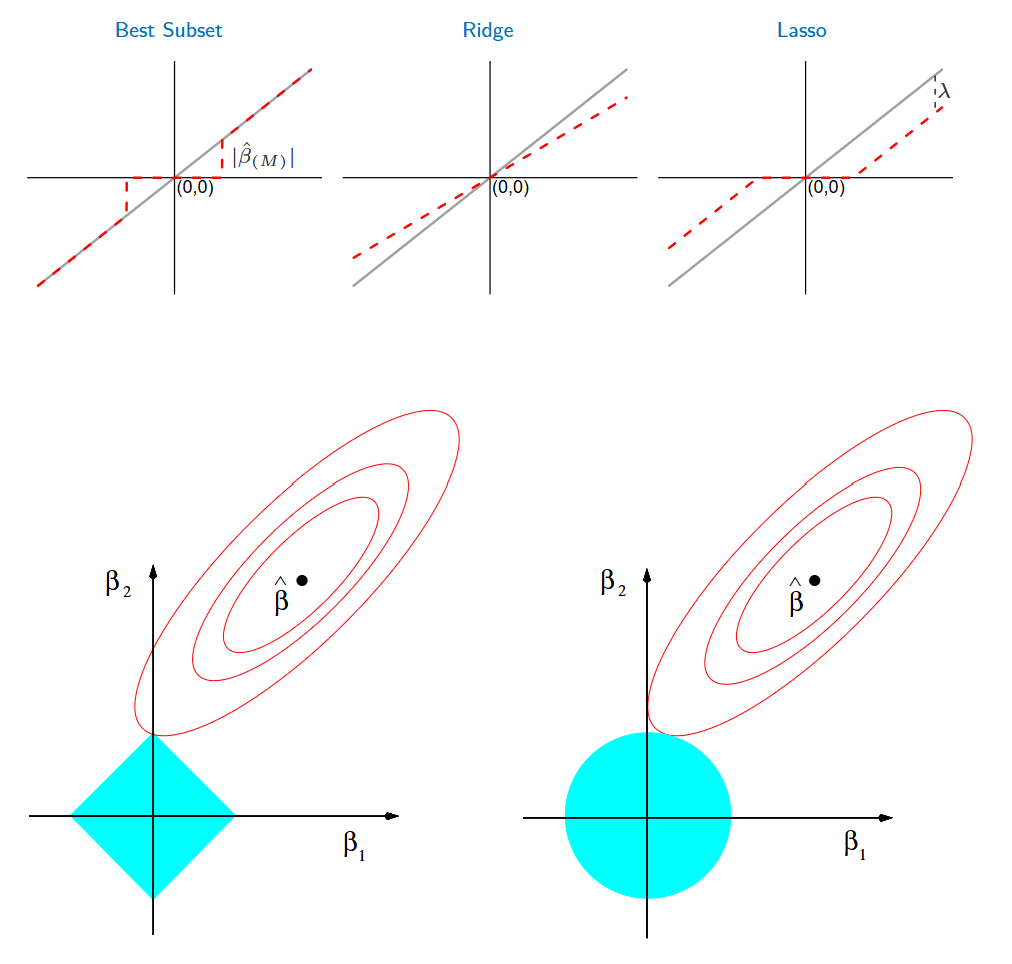
\includegraphics[width=0.85\textwidth]{Chapters/pic/ch_线性回归和最小二乘法/三种方法可视化.png}
    \caption{三种收缩方法的可视化比较。灰色 45° 线为 OLS 基准（无收缩）；红色虚线分别为最优子集（硬阈值）、岭回归（比例收缩）和 Lasso（软阈值）。横轴为 OLS 估计 $\hat{\beta}_j^{\text{ls}}$，纵轴为各方法的估计值。}
    \label{fig:three_methods}
\end{figure}

在非正交情形下，没有如此简洁的显式解，但\textbf{几何直觉}仍然成立。

\subsection{几何直观：$p=2$ 时的图形比较}

图 3.11 是理解 Lasso 与岭回归差异的最经典图示。考虑 $p=2$（两个预测变量）：

\begin{itemize}
    \item \textbf{RSS 等高线}：以 LS 估计 $\hat{\bm{\beta}}^{\text{ls}}$ 为中心的椭圆；
    \item \textbf{岭回归约束域}：圆盘 $\beta_1^2 + \beta_2^2 \le t$（光滑边界）；
    \item \textbf{Lasso 约束域}：菱形 $|\beta_1| + |\beta_2| \le t$（有四个尖角）。
\end{itemize}

两种方法都在寻找 RSS 等高线\textbf{首次触及}约束域边界的那一点。

\textbf{关键差异：}
\begin{itemize}
    \item 圆盘没有角落 → 切点几乎总在弧上 → $\beta_1 \neq 0$ 且 $\beta_2 \neq 0$；
    \item 菱形有尖角 → 如果切点落在角上（如 $\beta_1$ 轴上），则 $\beta_2 = 0$。
\end{itemize}

当 $p > 2$ 时，约束域变为菱形体 (rhomboid)，有大量的角、棱和面——
因此 Lasso 有很多机会将某些系数精确置零。

\subsubsection{图中三种元素的含义（逐层解读）}

为彻底理解这张图，把图中的元素拆成三层来看：

\begin{enumerate}[leftmargin=*]

\item \textbf{红色同心椭圆 —— RSS 等高线}

\[\text{RSS}(\bm{\beta}) = (\mathbf{y} - \mathbf{X}\bm{\beta})^\top(\mathbf{y} - \mathbf{X}\bm{\beta})\]

\begin{itemize}
    \item 椭圆中心 $\hat{\bm{\beta}}^{\text{ls}}$ 是\textbf{无约束最小二乘解}——RSS 的全局最小值点。
    \item 每一条椭圆线代表 RSS 取某一固定值；越靠近中心 RSS 越小，越远离 RSS 越大。
    \item 如果没有约束，最优解就是椭圆中心本身。
\end{itemize}

\item \textbf{蓝色区域 —— 约束范围（可行域）}

\begin{center}
\begin{tabular}{c|c|c}
\toprule
& \textbf{Lasso（左图）} & \textbf{Ridge（右图）} \\
\midrule
约束形式 & $|\beta_1| + |\beta_2| \le t$ & $\beta_1^2 + \beta_2^2 \le t^2$ \\
几何形状 & 菱形（$L_1$ 球） & 圆形（$L_2$ 球） \\
边界特征 & \textbf{有四个尖角}（在坐标轴上） & \textbf{处处光滑}，没有尖角 \\
\bottomrule
\end{tabular}
\end{center}

参数必须在蓝色区域内部（或边界上）取值——这是正则化施加的\textbf{硬约束}。

\item \textbf{最优解：椭圆首次\"碰到\"蓝色区域的那个点}

约束优化问题等价于从椭圆中心出发，\textbf{逐步扩大 RSS 椭圆的半径}。
椭圆扩大的过程中，\textbf{第一次触碰到蓝色区域边界}的那个点，就是约束下的最优解 $\hat{\bm{\beta}}^{\text{constrained}}$。

\end{enumerate}

\subsubsection{为什么 Lasso 产生零系数而 Ridge 不能？}

关键全在\textbf{尖角}上：

\begin{itemize}
    \item \textbf{Lasso（菱形）}：菱形在坐标轴上有四个尖角，例如 $(\beta_1, 0)$ 或 $(0, \beta_2)$。
    当 RSS 椭圆向外扩展时，\textbf{极易先碰到尖角}——此时交点恰好落在坐标轴上，意味着其中一个参数被精确压到 0。

    \item \textbf{Ridge（圆形）}：圆形处处光滑。RSS 椭圆与圆的切点几乎总在弧的内部——两坐标均非零。系数被压缩，但\textbf{从不精确为零}。
\end{itemize}

\[
\begin{array}{c}
\text{一句话总结：} \\
\text{Lasso 的 } L_1 \text{ 约束域有尖角，} \\
\text{RSS 椭圆碰到尖角时就自动做了变量选择——不重要的系数精确置零。}
\end{array}
\]

当 $p \gg 2$ 时，$L_1$ 约束域变为高维菱形体，拥有大量的角、棱和面，
Lasso 有更多机会将不重要的系数精确置零——这就是它在高维问题中表现优异的原因。

\subsection{一般 $L_q$ 惩罚与贝叶斯统一视角}

三种方法可以纳入一个统一的 $L_q$ 惩罚框架：
\begin{equation}\label{eq:Lq}
    \tilde{\bm{\beta}} = \argmin_{\bm{\beta}} \left\{
        \sum_{i=1}^{N} \Big(y_i - \beta_0 - \sum_{j=1}^{p} x_{ij}\beta_j\Big)^2
        + \lambda \sum_{j=1}^{p} |\beta_j|^q
    \right\}, \quad q \ge 0.
\end{equation}

不同 $q$ 值对应不同方法：

\begin{center}
\renewcommand{\arraystretch}{1.3}
\begin{tabular}{c|c|c|c}
\toprule
$q$ & \textbf{方法} & \textbf{先验分布} & \textbf{约束域形状} \\
\midrule
0   & 最优子集       & 尖峰-平板 (spike-and-slab) & 计数惩罚（非凸） \\
1   & Lasso          & 拉普拉斯 (双指数)          & 菱形（凸） \\
2   & 岭回归         & 高斯                       & 球（凸） \\
\bottomrule
\end{tabular}
\end{center}

\textbf{贝叶斯解读：} 将 $\sum |\beta_j|^q$ 视为 $\beta_j$ 的负对数先验密度，则：
\begin{itemize}
    \item $q=2$：高斯先验 $\beta_j \sim \mathcal{N}(0, \tau^2)$，$\lambda = \sigma^2/\tau^2$；
    \item $q=1$：拉普拉斯先验 $p(\beta_j) = \frac{1}{2\tau}\exp(-|\beta_j|/\tau)$，$\tau = 1/\lambda$；
    \item $q<1$：先验在坐标轴方向上集中更多质量——更容易产生零系数。
\end{itemize}

\subsubsection{推导：从最大后验 (MAP) 到正则化}

考虑线性模型 $y_i = \beta_0 + \sum_j x_{ij}\beta_j + \varepsilon_i$，$\varepsilon_i \sim \mathcal{N}(0, \sigma^2)$。
似然函数为：
\[
p(\mathbf{y} \mid \bm{\beta}) \propto \exp\!\left(-\frac{1}{2\sigma^2}\sum_{i=1}^{N}\big(y_i - \beta_0 - \sum_{j=1}^{p} x_{ij}\beta_j\big)^2\right).
\]

为 $\beta_j$ 引入独立先验 $p(\beta_j) \propto \exp(-|\beta_j|^q / \tau)$。由贝叶斯定理，后验：
\[
p(\bm{\beta} \mid \mathbf{y}) \propto p(\mathbf{y} \mid \bm{\beta}) \cdot \prod_{j=1}^{p} p(\beta_j).
\]

取负对数，最大化后验（MAP）等价于最小化：
\[
-\log p(\bm{\beta} \mid \mathbf{y})
= \underbrace{\frac{1}{2\sigma^2}\sum_{i=1}^{N}\big(y_i - \beta_0 - \sum_{j} x_{ij}\beta_j\big)^2}_{\text{RSS / } 2\sigma^2}
\;+\; \underbrace{\frac{1}{\tau}\sum_{j=1}^{p} |\beta_j|^q}_{\text{负对数先验}}
\;+\; \text{const}.
\]

乘以 $2\sigma^2$，令 $\lambda = 2\sigma^2 / \tau$，即得：
\[
\boxed{\;\hat{\bm{\beta}}^{\text{MAP}} = \argmin_{\bm{\beta}} \left\{
\text{RSS} + \lambda \sum_{j=1}^{p} |\beta_j|^q
\right\}\;}
\]

\textbf{这就是正则化框架}：惩罚系数 $\lambda$ 本质上编码了\emph{先验强度}（$\tau$ 小 $\Rightarrow$ $\lambda$ 大 $\Rightarrow$ 先验强 $\Rightarrow$ 强收缩）。

\subsubsection{为什么 $q=2$ 对应高斯，$q=1$ 对应拉普拉斯？}

核心对应关系：\textbf{$L_q$ 惩罚 $\; \leftrightarrow\;$ 指数幂分布族}

\[
p(\beta) \propto \exp(-|\beta|^q / \tau)
\]

具体展开：

\begin{center}
\renewcommand{\arraystretch}{1.8}
\small
\begin{tabular}{c|p{5.2cm}|p{3.2cm}|p{2.8cm}}
\toprule
$q$ & 先验密度形式 & 分布名称 & 在 0 处的形状 \\
\midrule
2 & $p(\beta) \propto \exp\!\big(-\frac{\beta^2}{2\tau^2}\big)$
   & $\mathcal{N}(0, \tau^2)$（高斯）
   & 光滑抛物线，可微 \\
1 & $p(\beta) \propto \exp\!\big(-\frac{|\beta|}{\tau}\big)$
   & $\operatorname{Laplace}(0, \tau)$（拉普拉斯/双指数）
   & \textbf{尖峰}，在 0 处不可微 \\
0 & $p(\beta)$ 为 0 处点质量 + 平坦尾部的混合
   & 尖峰-平板 (spike-and-slab)
   & 极端集中 \\
\bottomrule
\end{tabular}
\end{center}

\textbf{几何直觉：为什么拉普拉斯先验导致稀疏？}

\begin{itemize}
    \item \textbf{高斯先验}（$q=2$）：在 $\beta_j=0$ 附近光滑、平缓——先验并不特别\emph{偏爱}零值，
    后验众数几乎不会精确落在 0 上。
    \item \textbf{拉普拉斯先验}（$q=1$）：在 $\beta_j=0$ 处有一个\textbf{尖峰}——
    先验强烈倾向于零。只要数据没有压倒性证据，MAP 估计就会精确落在 0。
\end{itemize}

换个角度：拉普拉斯分布的尾部比高斯\emph{更重}——如果 $\beta_j$ 真的非零，
它允许系数取到较大值而不被过度惩罚。这正是 Lasso 的优势：
\textbf{对小系数"赶尽杀绝"（压到 0），对大系数"网开一面"（只减去常数 $\lambda$）}。

\textbf{注意：} 以上都是后验\textbf{众数}（mode）。岭回归同时也是后验均值（因为高斯后验对称），
但 Lasso 和最优子集的后验均值不等于后验众数。

\textbf{为什么 $q=1$ 是"神奇"的值？}
\begin{itemize}
    \item $q=1$ 是使得约束域\textbf{凸}的最小 $q$（$q<1$ 时为非凸，优化困难）；
    \item $q=1$ 是使得约束域\textbf{在坐标轴上有尖角}的最大 $q$（$q>1$ 时在零点可微，无尖角 → 无稀疏性）。
\end{itemize}
因此 $q=1$ 是唯一同时满足\textbf{凸性（易于优化）+ 稀疏性（可产生零系数）}的值。

\subsection{弹性网 (Elastic Net)}

$q \in (1, 2)$ 的 $L_q$ 惩罚是岭回归和 Lasso 的折中，但在零点处可微（无尖角），
因此\textbf{不能产生稀疏解}。Zou \& Hastie (2005) 提出了弹性网惩罚：
\begin{equation}\label{eq:elastic_net}
    \lambda \sum_{j=1}^{p} \Big(\alpha \beta_j^2 + (1-\alpha) |\beta_j|\Big).
\end{equation}

弹性网 = 岭回归（$L_2$）+ Lasso（$L_1$）的\textbf{凸组合}，通过 $\alpha \in [0,1]$ 调节两者权重：
\begin{itemize}
    \item $\alpha = 0$：退化为 Lasso；
    \item $\alpha = 1$：退化为岭回归；
    \item 中间值：同时具备两者的优点。
\end{itemize}

\textbf{弹性网的优势：}
\begin{itemize}
    \item \textbf{变量选择}：$L_1$ 部分保留尖角 → 可产生稀疏解，像 Lasso；
    \item \textbf{处理相关变量}：$L_2$ 部分使高度相关的变量系数被一起收缩，像岭回归；
    \item \textbf{计算优势}：比一般的 $L_q$（$1<q<2$）更容易优化；
    \item \textbf{高维适用}：当 $p \gg N$ 时，Lasso 最多选 $N$ 个变量，弹性网可以选更多。
\end{itemize}

\subsection{最小角回归 (LAR)——Lasso 的高效算法}

Lasso 没有闭式解，如何高效计算整个解路径（随 $\lambda$ 变化的所有 $\hat{\bm{\beta}}^{\text{lasso}}$）？
答案是\textbf{最小角回归 (Least Angle Regression, LAR)}（Efron et al., 2004）。

\subsubsection{与前向逐步的对比}

\begin{itemize}
    \item \textbf{前向逐步：} 每次选出与残差最相关的变量，然后\textbf{完全拟合}该变量（调整到 LS 值），
    再找下一个变量。偏好过于激进——一旦加入就"吃饱"；
    \item \textbf{LAR：} 每次选出与残差最相关的变量，但只让它的系数沿 LS 方向移动，
    \textbf{直到另一个变量与残差的相关性追上来}。然后两者一起移动，保持相关性相等。
    这是一种"民主"的前向逐步——每个变量只得到它"应得"的那份。
\end{itemize}

\subsubsection{算法直觉}

\begin{enumerate}[label=第 \arabic* 步：, leftmargin=*]
    \item 所有系数初始化为 0，残差 $\mathbf{r} = \mathbf{y} - \bar{y}$；
    \item 找到与 $\mathbf{r}$ 最相关的变量 $\mathbf{x}_{j_1}$；
    \item 将 $\hat{\beta}_{j_1}$ 从 0 向 LS 方向移动。随 $\hat{\beta}_{j_1}$ 增大，
    $\mathbf{x}_{j_1}$ 与残差的相关性逐渐下降；
    \item 当某个其他变量 $\mathbf{x}_{j_2}$ 与残差的相关性追上来（等于 $\mathbf{x}_{j_1}$ 的），
    将其加入活跃集；
    \item 现在同时移动 $\hat{\beta}_{j_1}$ 和 $\hat{\beta}_{j_2}$，保持两者与残差的相关性相等且逐步减小；
    \item 重复，直到所有变量都进入模型（或残差为 0）。
\end{enumerate}

\textbf{与 Lasso 的深刻联系：} LAR 稍加修改（当一个系数穿过零时从活跃集中移除该变量），
就\textbf{精确等价于 Lasso 的解路径}。因此 LAR 提供了一种计算整个 Lasso 路径的高效方法——
计算量与单次 LS 拟合相当。

\subsection{小结：收缩方法谱系}

\[
\begin{array}{c|c|c|c}
\toprule
& \textbf{子集选择} & \textbf{岭回归} & \textbf{Lasso} \\
\midrule
\text{操作方式}    & 离散：选/不选 & 连续：压缩 & 连续：压缩+置零 \\
\text{解的线性性}  & \times & \checkmark & \times \\
\text{稀疏性}      & \checkmark & \times & \checkmark \\
\text{变量选择}     & \checkmark & \times & \checkmark \\
\text{方差}         & 高（离散决策） & 低 & 中等 \\
\text{偏差}         & 较低 & 有偏 & 有偏 \\
\text{高维适用}     & $p$ 不太大 & \checkmark \; 总是可逆 & \checkmark \\
\text{贝叶斯解释}   & 尖峰先验 (spike) & 高斯先验 & 拉普拉斯先验 \\
\bottomrule
\end{array}
\]

\textbf{核心教训：}
\begin{itemize}
    \item 子集选择的离散性导致高方差——数据微小扰动可能选出完全不同的子集；
    \item 岭回归通过 $L_2$ 惩罚连续收缩，方差低但无稀疏性；
    \item Lasso 通过 $L_1$ 惩罚同时实现收缩和变量选择——是现代高维统计的基准方法；
    \item 正交情形下三者有统一显式解：硬阈值 / 比例收缩 / 软阈值；
    \item LAR 为 Lasso 提供了高效的计算路径——增量式地、"民主"地添加变量；
    \item 弹性网结合 $L_1+L_2$，在有相关变量和高维场景下优于纯 Lasso。
\end{itemize}

% ============================================================
%  § 使用导出输入方向的方法 (ESL §3.5)
% ============================================================
\section{使用导出输入方向的方法 (Derived Input Directions)}

前两节（子集选择和收缩方法）通过控制系数来正则化。
另一种思路是：\textbf{先把原始变量降维，在低维空间做回归。}
这是一种``先压缩、再回归''的策略。

\subsection{主成分回归 (PCR)}

\begin{definition}[主成分回归]
PCR 的执行步骤：
\begin{enumerate}[label=第 \arabic* 步：, leftmargin=*]
    \item 对 $\mathbf{X}$（中心化后）做 PCA，取前 $M$ 个主成分 $\mathbf{z}_1, \dots, \mathbf{z}_M$；
    \item 将 $\mathbf{y}$ 对 $\mathbf{z}_1, \dots, \mathbf{z}_M$ 做普通最小二乘。
\end{enumerate}
\end{definition}

\textbf{关键特征：}
\begin{itemize}
    \item 主成分 $\mathbf{z}_m = \mathbf{X}\mathbf{v}_m$ 的选择\textbf{只依赖 $\mathbf{X}$，不依赖 $\mathbf{y}$}；
    \item PCR 丢弃了低方差方向——这些方向上信噪比通常最差；
    \item 但与 PLS 不同，PCR 不考虑 $\mathbf{y}$——高方差方向不一定预测力强。
\end{itemize}

\subsection{偏最小二乘 (PLS)}

PLS 的思想是：\textbf{在构造降维方向时同时考虑 $\mathbf{x}$ 的方差和与 $\mathbf{y}$ 的相关性。}

\begin{definition}[PLS 算法 (Algorithm 3.3)]
\begin{enumerate}[label=第 \arabic* 步：, leftmargin=*]
    \item 标准化所有 $\mathbf{x}_j$（均值 0，方差 1），设 $\hat{\mathbf{y}}^{(0)} = \bar{y}\mathbf{1}$；
    \item 对 $m = 1, 2, \dots, p$：
    \begin{enumerate}
        \item[(a)] $\mathbf{z}_m = \sum_{j=1}^{p} \hat{\phi}_{mj} \mathbf{x}_j^{(m-1)}$，其中
        $\hat{\phi}_{mj} = \langle \mathbf{x}_j^{(m-1)}, \mathbf{y} \rangle$；
        \item[(b)] $\hat{\theta}_m = \langle \mathbf{z}_m, \mathbf{y} \rangle / \langle \mathbf{z}_m, \mathbf{z}_m \rangle$；
        \item[(c)] $\hat{\mathbf{y}}^{(m)} = \hat{\mathbf{y}}^{(m-1)} + \hat{\theta}_m \mathbf{z}_m$；
        \item[(d)] 将每个 $\mathbf{x}_j^{(m-1)}$ 关于 $\mathbf{z}_m$ 正交化：
        $\mathbf{x}_j^{(m)} = \mathbf{x}_j^{(m-1)} - [\langle \mathbf{z}_m, \mathbf{x}_j^{(m-1)} \rangle / \langle \mathbf{z}_m, \mathbf{z}_m \rangle] \mathbf{z}_m$。
    \end{enumerate}
    \item 输出拟合序列 $\{\hat{\mathbf{y}}^{(m)}\}_{m=1}^{p}$。
\end{enumerate}
\end{definition}

\textbf{PLS 与 PCR 的核心区别：}
\begin{itemize}
    \item \textbf{PCR：} 选择方向只最大化 $\Var(\mathbf{X}\bm{\alpha})$（\textbf{不管 $\mathbf{y}$}）；
    \item \textbf{PLS：} 选择方向最大化 $\Corr^2(\mathbf{y}, \mathbf{X}\bm{\alpha}) \cdot \Var(\mathbf{X}\bm{\alpha})$
    （\textbf{同时考虑方差和相关性}）。
\end{itemize}

实证研究表明：PLS 中方差项倾向于占主导地位，因此 PLS 的表现与岭回归和 PCR
\textbf{非常相似}。Frank \& Friedman (1993) 结论：就最小化预测误差而言，
岭回归通常优于变量子集选择、PCR 和 PLS，但优势仅略微。

\textbf{有趣的事实：} 如果 $\mathbf{X}$ 的列正交，PLS 在 $m=1$ 步后就得到 LS 解——
后续步骤没有效果（因为 $\hat{\phi}_{mj}=0,\; m>1$）。
PLS 系数序列 $m=1,2,\dots,p$ 恰好是计算 LS 解的\textbf{共轭梯度序列}。

\subsection{PCR 与 PLS 的优化问题}

第 $m$ 个 PCR 方向 $\mathbf{v}_m$ 求解：
\begin{equation}
    \max_{\bm{\alpha}} \Var(\mathbf{X}\bm{\alpha})
    \quad \text{s.t.} \quad \|\bm{\alpha}\|=1,\; \bm{\alpha}^\top \mathbf{S} \mathbf{v}_\ell = 0,\; \ell=1,\dots,m-1.
\end{equation}

第 $m$ 个 PLS 方向 $\hat{\bm{\phi}}_m$ 求解：
\begin{equation}
    \max_{\bm{\alpha}} \Corr^2(\mathbf{y}, \mathbf{X}\bm{\alpha}) \cdot \Var(\mathbf{X}\bm{\alpha})
    \quad \text{s.t.} \quad \|\bm{\alpha}\|=1,\; \bm{\alpha}^\top \mathbf{S} \hat{\bm{\phi}}_\ell = 0,\; \ell=1,\dots,m-1.
\end{equation}

% ============================================================
%  Q&A: PLS 正交投影视角 + 完整例子 + 为什么同时考虑方差和相关性
% ============================================================
\subsection{深入理解 PLS：正交投影、实例与动机}

\subsubsection{从正交投影看 PLS}

PLS 的每一步本质上在做两件事：\textbf{投影 + 剔除}。理解它的关键是把它和 Gram-Schmidt 正交化做类比。

\medskip
\noindent
\textbf{回顾 Gram-Schmidt（纯 $\mathbf{X}$ 视角）：}

给定向量 $\mathbf{x}_1, \mathbf{x}_2, \dots, \mathbf{x}_p$，Gram-Schmidt 依次构造正交基：
\[
\mathbf{z}_1 = \mathbf{x}_1,\quad
\mathbf{z}_2 = \mathbf{x}_2 - \frac{\langle \mathbf{z}_1, \mathbf{x}_2 \rangle}{\langle \mathbf{z}_1, \mathbf{z}_1 \rangle}\mathbf{z}_1,\quad
\mathbf{z}_3 = \mathbf{x}_3 - \frac{\langle \mathbf{z}_1, \mathbf{x}_3 \rangle}{\langle \mathbf{z}_1, \mathbf{z}_1 \rangle}\mathbf{z}_1
- \frac{\langle \mathbf{z}_2, \mathbf{x}_3 \rangle}{\langle \mathbf{z}_2, \mathbf{z}_2 \rangle}\mathbf{z}_2,\quad \dots
\]

每一步把新向量投影到前面所有 $\mathbf{z}$ 的正交补上——\textbf{提取``前面还没用过的信息''}。

\medskip
\noindent
\textbf{PLS 的投影逻辑（$\mathbf{X}$ + $\mathbf{y}$ 联合视角）：}

PLS 把同样的正交化思想用在 $\mathbf{X}$ 上，但顺序由 $\mathbf{y}$ 来定：

\begin{center}
\fbox{%
\begin{minipage}{0.9\textwidth}
\textbf{第 $m$ 步的核心操作：}

\begin{enumerate}[label=(\arabic*), leftmargin=*]
    \item \textbf{选方向权重：} 计算每个 $\mathbf{x}_j^{(m-1)}$（经前面 $m-1$ 步正交化后的残差变量）与 $\mathbf{y}$ 的内积：
    $\hat{\phi}_{mj} = \langle \mathbf{x}_j^{(m-1)}, \mathbf{y} \rangle$。
    这是 $\mathbf{x}_j^{(m-1)}$ 与 $\mathbf{y}$ 的协方差（在零均值下）。
    
    \item \textbf{构造方向：} $\mathbf{z}_m = \sum_j \hat{\phi}_{mj} \mathbf{x}_j^{(m-1)}$，
    相当于把当前所有``剩余变量''按它们与 $\mathbf{y}$ 的协方差加权组合成新方向。
    
    \item \textbf{$\mathbf{y}$ 对 $\mathbf{z}_m$ 投影：} $\hat{\theta}_m = \langle \mathbf{z}_m, \mathbf{y} \rangle / \langle \mathbf{z}_m, \mathbf{z}_m \rangle$，
    这就是 $\mathbf{y}$ 在 $\mathbf{z}_m$ 上的最小二乘回归系数（无截距）。更新拟合：
    $\hat{\mathbf{y}}^{(m)} = \hat{\mathbf{y}}^{(m-1)} + \hat{\theta}_m \mathbf{z}_m$。
    
    \item \textbf{剔除已用信息：} 将每个 $\mathbf{x}_j^{(m-1)}$ 对 $\mathbf{z}_m$ 做正交投影，
    去掉 $\mathbf{z}_m$ 分量：
    \[
        \mathbf{x}_j^{(m)} = \mathbf{x}_j^{(m-1)} - \frac{\langle \mathbf{z}_m, \mathbf{x}_j^{(m-1)} \rangle}{\langle \mathbf{z}_m, \mathbf{z}_m \rangle} \mathbf{z}_m.
    \]
    这一步保证 $\mathbf{z}_{m+1}$（下一轮构造的方向）与 $\mathbf{z}_m$ 正交。
\end{enumerate}
\end{minipage}}
\end{center}

\medskip
\noindent
\textbf{一句话理解：} PLS = Gram-Schmidt 正交化，但每次选哪个变量先做，
由``谁和 $\mathbf{y}$ 协方差大''来决定，而非由``谁方差大''来决定。

\medskip
\noindent
\textbf{投影矩阵视角：}

由于 $\mathbf{z}_m$ 是 $\mathbf{x}_j^{(m-1)}$ 的线性组合，而 $\mathbf{x}_j^{(m-1)}$ 本身
是原始 $\mathbf{X}$ 的线性组合（经过 $m-1$ 次正交化），所以 $\mathbf{z}_m$ 最终是 $\mathbf{X}$ 的线性组合：
\[
    \mathbf{z}_m = \mathbf{X} \mathbf{w}_m,
\]
其中 $\mathbf{w}_m$ 可由 PLS 权重反向推导。所有 $\mathbf{z}_1, \dots, \mathbf{z}_M$ 张成的子空间是
$\mathbf{X}$ 列空间的子空间。最终的拟合 $\hat{\mathbf{y}}^{(M)}$ 是 $\mathbf{y}$ 在这个子空间上的投影。

\subsubsection{完整数值例子}

下面用一个极简数据集（$N=4,\; p=2$）手动走一遍 PLS。

\begin{center}
\renewcommand{\arraystretch}{1.3}
\begin{tabular}{c|ccc}
\toprule
$i$ & $y_i$ & $x_{i1}$ & $x_{i2}$ \\
\midrule
1 & 3  & 1 & 2 \\
2 & 5  & 2 & 2 \\
3 & 7  & 3 & 5 \\
4 & 9  & 4 & 3 \\
\bottomrule
\end{tabular}
\end{center}

\medskip
\noindent
\textbf{第 0 步：标准化。}

中心化：
\[
\bar{y} = 6,\quad \bar{x}_1 = 2.5,\quad \bar{x}_2 = 3.0.
\]
\[
\mathbf{y}^{(0)} = \begin{pmatrix} -3 \\ -1 \\ 1 \\ 3 \end{pmatrix},\quad
\mathbf{x}_1^{(0)} = \begin{pmatrix} -1.5 \\ -0.5 \\ 0.5 \\ 1.5 \end{pmatrix},\quad
\mathbf{x}_2^{(0)} = \begin{pmatrix} -1 \\ -1 \\ 2 \\ 0 \end{pmatrix}.
\]

缩放到单位范数（$\|\mathbf{x}_j\| = 1$）：
\[
\|\mathbf{x}_1^{(0)}\| = \sqrt{1.5^2 + 0.5^2 + 0.5^2 + 1.5^2} = \sqrt{5} \approx 2.236,\quad
\|\mathbf{x}_2^{(0)}\| = \sqrt{1^2 + 1^2 + 2^2 + 0^2} = \sqrt{6} \approx 2.449.
\]
\[
\mathbf{x}_1^{(0)} \leftarrow \frac{1}{\sqrt{5}}\begin{pmatrix} -1.5 \\ -0.5 \\ 0.5 \\ 1.5 \end{pmatrix},\quad
\mathbf{x}_2^{(0)} \leftarrow \frac{1}{\sqrt{6}}\begin{pmatrix} -1 \\ -1 \\ 2 \\ 0 \end{pmatrix}.
\]

$\hat{\mathbf{y}}^{(0)} = \bar{y}\,\mathbf{1} = (6,6,6,6)^\top$。

\medskip
\noindent
\textbf{第 1 步 ($m=1$)：}

\begin{enumerate}[label=(\alph*), leftmargin=*]
    \item 计算权重：
    \[
        \hat{\phi}_{11} = \langle \mathbf{x}_1^{(0)}, \mathbf{y}^{(0)} \rangle
        = \frac{(-1.5)(-3) + (-0.5)(-1) + 0.5\cdot 1 + 1.5\cdot 3}{\sqrt{5}}
        = \frac{4.5 + 0.5 + 0.5 + 4.5}{\sqrt{5}} = \frac{10}{\sqrt{5}} \approx 4.47.
    \]
    \[
        \hat{\phi}_{12} = \langle \mathbf{x}_2^{(0)}, \mathbf{y}^{(0)} \rangle
        = \frac{(-1)(-3) + (-1)(-1) + 2\cdot 1 + 0\cdot 3}{\sqrt{6}}
        = \frac{3 + 1 + 2 + 0}{\sqrt{6}} = \frac{6}{\sqrt{6}} \approx 2.45.
    \]
    
    \item 构造 $\mathbf{z}_1$：
    \[
        \mathbf{z}_1 = \hat{\phi}_{11}\mathbf{x}_1^{(0)} + \hat{\phi}_{12}\mathbf{x}_2^{(0)}
        = \frac{10}{\sqrt{5}}\mathbf{x}_1^{(0)} + \frac{6}{\sqrt{6}}\mathbf{x}_2^{(0)}.
    \]
    
    直接写出 $\mathbf{z}_1$ 的坐标（代入标准化前的中心化值更方便）——等价于用原始中心化变量：
    $\mathbf{z}_1 \propto 10\cdot \tilde{\mathbf{x}}_1 + 6\cdot \tilde{\mathbf{x}}_2$，其中 $\tilde{\mathbf{x}}_j$ 为中心化后的原始值。
    \[
        \mathbf{z}_1 \propto 10\!\begin{pmatrix} -1.5 \\ -0.5 \\ 0.5 \\ 1.5 \end{pmatrix}
        + 6\!\begin{pmatrix} -1 \\ -1 \\ 2 \\ 0 \end{pmatrix}
        = \begin{pmatrix} -21 \\ -11 \\ 17 \\ 15 \end{pmatrix}.
    \]
    
    归一化：$\|\mathbf{z}_1\| = \sqrt{21^2 + 11^2 + 17^2 + 15^2} = \sqrt{1076}$。实际 PLS 中不必须单位化，
    关键是计算 $\hat{\theta}_1$：
    
    \item 计算回归系数：
    \[
        \hat{\theta}_1 = \frac{\langle \mathbf{z}_1, \mathbf{y}^{(0)} \rangle}{\langle \mathbf{z}_1, \mathbf{z}_1 \rangle}
        = \frac{(-21)(-3) + (-11)(-1) + 17\cdot 1 + 15\cdot 3}{1076}
        = \frac{63 + 11 + 17 + 45}{1076} = \frac{136}{1076} \approx 0.1264.
    \]
    
    \item 更新拟合（$\mathbf{y}$ 的投影）：
    \[
        \hat{\mathbf{y}}^{(1)} = \hat{\mathbf{y}}^{(0)} + \hat{\theta}_1 \mathbf{z}_1
        = \begin{pmatrix} 6 \\ 6 \\ 6 \\ 6 \end{pmatrix}
        + 0.1264 \begin{pmatrix} -21 \\ -11 \\ 17 \\ 15 \end{pmatrix}
        \approx \begin{pmatrix} 3.35 \\ 4.61 \\ 8.15 \\ 7.90 \end{pmatrix}.
    \]
    
    残差 $\mathbf{y}^{(1)} = \mathbf{y} - \hat{\mathbf{y}}^{(1)} \approx ( -0.35,\; 0.39,\; -1.15,\; 1.10)^\top$。
    
    \item 正交化 $\mathbf{x}_j$（剔除 $\mathbf{z}_1$ 分量）：
    \[
        \mathbf{x}_1^{(1)} = \mathbf{x}_1^{(0)} - \frac{\langle \mathbf{z}_1, \mathbf{x}_1^{(0)} \rangle}{\langle \mathbf{z}_1, \mathbf{z}_1 \rangle} \mathbf{z}_1,
        \qquad
        \mathbf{x}_2^{(1)} = \mathbf{x}_2^{(0)} - \frac{\langle \mathbf{z}_1, \mathbf{x}_2^{(0)} \rangle}{\langle \mathbf{z}_1, \mathbf{z}_1 \rangle} \mathbf{z}_1.
    \]
\end{enumerate}

\medskip
\noindent
\textbf{第 2 步 ($m=2$)：}

用 $\mathbf{x}_1^{(1)}, \mathbf{x}_2^{(1)}$ 和残差 $\mathbf{y}^{(1)}$（$\mathbf{y}$ 中尚未被 $\mathbf{z}_1$ 解释的部分）
重复上述过程。构造 $\mathbf{z}_2$（与 $\mathbf{z}_1$ 正交），将 $\mathbf{y}^{(1)}$ 投影到 $\mathbf{z}_2$ 上，
更新拟合。此时 $\hat{\mathbf{y}}^{(2)}$ 接近 $\mathbf{y}$ 在 $\mathbf{X}$ 列空间上的完整投影。

\medskip
\noindent
\textbf{观察：}
\begin{itemize}
    \item $\mathbf{z}_1$ 里，$x_1$ 的权重（10）大于 $x_2$（6）——因为 $x_1$ 与 $y$ 的协方差更大；
    \item 经过第 1 步正交化, $\mathbf{x}_j^{(1)} \perp \mathbf{z}_1$——第 2 步只会用到``$\mathbf{z}_1$ 没吸收的信息''；
    \item 这和 Gram-Schmidt 一模一样，只是顺序由协方差驱动。
\end{itemize}

\subsubsection{为什么同时考虑方差和相关性？}

PLS 的优化准则可以化简：
\[
    \Corr^2(\mathbf{y}, \mathbf{X}\bm{\alpha}) \cdot \Var(\mathbf{X}\bm{\alpha})
    = \frac{\Cov^2(\mathbf{y}, \mathbf{X}\bm{\alpha})}{\Var(\mathbf{y})\Var(\mathbf{X}\bm{\alpha})}
      \cdot \Var(\mathbf{X}\bm{\alpha})
    = \frac{\Cov^2(\mathbf{y}, \mathbf{X}\bm{\alpha})}{\Var(\mathbf{y})}.
\]

由于 $\Var(\mathbf{y})$ 是常数，这等价于最大化 $|\Cov(\mathbf{y}, \mathbf{X}\bm{\alpha})|$。
也就是说，PLS 的准则在数学上退化为简单的\textbf{协方差最大化}。
那为什么 ESL 要写成``相关性 $\times$ 方差''这种貌似复杂的形式？

\medskip
\noindent
\textbf{答案：两个极端失败案例能说明一切。}

\begin{center}
\renewcommand{\arraystretch}{1.5}
\begin{tabular}{p{3.5cm}|p{5cm}|p{5cm}}
\toprule
& \textbf{只最大化相关性 (CCA 方向)} & \textbf{只最大化方差 (PCA 方向)} \\
\midrule
\textbf{准则}    & $\max \Corr^2(\mathbf{y}, \mathbf{X}\bm{\alpha})$ & $\max \Var(\mathbf{X}\bm{\alpha})$ \\
\midrule
\textbf{会怎样}  & 可能选到一个与 $\mathbf{y}$ 高度相关、但 $\mathbf{X}\bm{\alpha}$ 波动\textbf{极小}的方向
                   → $\hat{\theta}$ 估计极不稳定（方差巨大）&
                   可能选到一个 $\mathbf{X}\bm{\alpha}$ 方差大、但与 $\mathbf{y}$ 完全不相干的方向
                   → 白做，预测力为零 \\
\midrule
\textbf{极端例子} & $\mathbf{x}_1$ 与 $\mathbf{y}$ 相关 $0.9$，但 $\Var(\mathbf{x}_1) = 0.001$；
                   $\hat{\theta}$ 的方差 $\propto 1/\|\mathbf{z}\|^2 \to \infty$ &
                   $\mathbf{x}_2$ 方差极大但 $\Corr(\mathbf{x}_2, \mathbf{y}) \approx 0$；
                   这个方向对预测毫无用处 \\
\midrule
\textbf{PLS 的做法} & \multicolumn{2}{p{10cm}}{\textbf{同时要求两者：} $\Corr^2 \cdot \Var = \Cov^2 / \Var(\mathbf{y})$ —— 既不接受方差太小的方向（不稳定），也不接受相关性太弱的方向（无预测力）} \\
\bottomrule
\end{tabular}
\end{center}

\medskip
\noindent
\textbf{更深入的理解——为什么恰好是协方差？}

协方差 $\Cov(\mathbf{y}, \mathbf{X}\bm{\alpha}) = \rho \cdot \sigma_y \cdot \sigma_{\mathbf{X}\bm{\alpha}}$
本身就是``相关性 $\times$ 标准差''：
\[
    \Cov = \underbrace{\Corr}_{\text{关系强度}} \;\times\;
           \underbrace{\sigma_y}_{\text{固定常数}} \;\times\;
           \underbrace{\sigma_{\mathbf{X}\bm{\alpha}}}_{\text{信号强度}}.
\]

所以 PLS 选的方向是在\textbf{相关性}和\textbf{信号强度}之间取得平衡：
\begin{itemize}
    \item 信号太弱（$\sigma_{\mathbf{X}\bm{\alpha}}$ 小）→ 即使相关性高也不可靠；
    \item 相关性太弱（$\rho \approx 0$）→ 即使信号强也与 $\mathbf{y}$ 无关。
\end{itemize}

\textbf{这就是为什么 PLS 的准则写成 $\Corr^2 \cdot \Var$——它清楚地表达了这两个成分的权衡，
尽管数学上退化为协方差最大化。}

与 PCR 的对比更加清楚：
\begin{itemize}
    \item PCR：$\max \Var(\mathbf{X}\bm{\alpha})$ → 只关心 $\mathbf{X}$ 自己的变异结构，完全忽略 $\mathbf{y}$。
    如果 $\mathbf{y}$ 主要依赖低方差成分（如光谱学中痕量成分），PCR 会直接扔掉它。
    \item PLS：$\max \Cov(\mathbf{y}, \mathbf{X}\bm{\alpha})$ → 取 $\mathbf{X}$ 的变异和 $\mathbf{y}$ 的交集。
    不浪费自由度在``方差大但与 $\mathbf{y}$ 无关''的方向上。
\end{itemize}

\medskip
\noindent
\textbf{一句话总结：}
PLS 的准则看似是两个量的乘积，实际就是协方差最大化——它要的是 \textbf{``$\mathbf{X}$ 中与 $\mathbf{y}$ 有关系的那部分变异''}，
PCR 要的是``$\mathbf{X}$ 中变异最大的那部分''，而不管变异是否与 $\mathbf{y}$ 有关。

\medskip
\noindent
\textbf{追问：按协方差大小选方向，会不会让与 $\mathbf{y}$ 几乎无关的变量永远被忽略？}

这恰恰是 PLS 设计中最精妙的地方——\textbf{正交化步骤让变量有``第二次机会''。}

关键不在于单个变量在第 1 步权重有多大，而在于\textbf{第 $m$ 步用的是什么变量}。
第 $m$ 步使用的 $\mathbf{x}_j^{(m-1)}$ 不是原始 $\mathbf{x}_j$，而是\textbf{经过前 $m-1$ 轮正交化后的残差}：

\[
    \mathbf{x}_j^{(m-1)} = \mathbf{x}_j - \sum_{\ell=1}^{m-1} \frac{\langle \mathbf{z}_\ell, \mathbf{x}_j \rangle}{\langle \mathbf{z}_\ell, \mathbf{z}_\ell \rangle} \mathbf{z}_\ell.
\]

这意味着：

\begin{center}
\fbox{%
\begin{minipage}{0.9\textwidth}
\textbf{三种典型情况：}

\begin{enumerate}[label=\textbf{情况 \arabic*：}, leftmargin=*]
    \item \textbf{$\mathbf{x}_j$ 与 $\mathbf{y}$ 边缘协方差很大} → 第 1 步权重高，直接被大量纳入 $\mathbf{z}_1$。
    好的——这正是我们想要的。
    
    \item \textbf{$\mathbf{x}_j$ 与 $\mathbf{y}$ 边缘协方差很小，但与某个已被纳入的 $\mathbf{x}_k$ 高度相关} →
    第 1 步权重小，但正交化后 $\mathbf{x}_j^{(1)}$ 很小（因为大部分已被 $\mathbf{z}_1$ 剥离）。
    后续步骤中它与残差 $\mathbf{y}^{(m)}$ 的协方差仍然很小 →
    \textbf{最终被忽略。这是对的：它的信息已经被 $\mathbf{x}_k$ 代表了。}
    
    \item \textbf{$\mathbf{x}_j$ 与 $\mathbf{y}$ 边缘协方差很小，但与已纳入变量不相关} →
    第 1 步权重小。但正交化几乎不影响它（$\mathbf{x}_j^{(1)} \approx \mathbf{x}_j$）。
    第 1 步后，$\mathbf{y}^{(1)} = \mathbf{y} - \hat{\theta}_1\mathbf{z}_1$ 中与 $\mathbf{x}_j$ 有关的分量
    \textbf{仍然在残差里}——因此第 2 步时 $\langle \mathbf{x}_j^{(1)}, \mathbf{y}^{(1)} \rangle$ 和
    $\langle \mathbf{x}_j, \mathbf{y} \rangle$ 几乎一样大。
    如果其他变量的协方差在第 1 步已被大量消耗，$\mathbf{x}_j$ 在第 2 步就会\textbf{脱颖而出}。
    \textbf{这就是``第二次机会''。}
\end{enumerate}
\end{minipage}}
\end{center}

\medskip
\noindent
\textbf{用一个具体例子说明：}

假设 $p=3$，真实模型为 $y = 2x_1 + 1.5x_3 + \varepsilon$，且 $x_1$ 与 $x_2$ 高度相关（$r \approx 0.9$），
$x_3$ 与 $x_1, x_2$ 均独立。

第 1 步的边际协方差大小排序可能是：
\[
    |\Cov(\mathbf{x}_1, \mathbf{y})| > |\Cov(\mathbf{x}_2, \mathbf{y})| > |\Cov(\mathbf{x}_3, \mathbf{y})|.
\]

$\mathbf{x}_2$ 的协方差较大，不是因为 $\mathbf{x}_2$ 本身对 $y$ 有因果效应，而是因为它与 $\mathbf{x}_1$ 高度相关——
$\mathbf{x}_2$ ``搭了 $\mathbf{x}_1$ 的便车''。$\mathbf{x}_3$ 虽然真实系数是 $1.5$，但因为方差可能较小，
边际协方差排在最后。

\textbf{第 1 步后：}
\begin{itemize}
    \item $\mathbf{z}_1$ 主要捕获了 $\mathbf{x}_1$ 和 $\mathbf{x}_2$ 的共同变异；
    \item $\mathbf{x}_1^{(1)}$ 和 $\mathbf{x}_2^{(1)}$ 都变得很小（大部分已被剥离）；
    \item $\mathbf{x}_3^{(1)} \approx \mathbf{x}_3$（几乎未被触及，因为它与 $\mathbf{z}_1$ 正交）。
\end{itemize}

\textbf{第 2 步：}
\begin{itemize}
    \item $\mathbf{y}^{(1)}$ 中 $\mathbf{x}_3$ 的贡献纹丝未动；
    \item 此时 $\langle \mathbf{x}_3^{(1)}, \mathbf{y}^{(1)} \rangle \approx \langle \mathbf{x}_3, \mathbf{y} \rangle$；
    \item 而 $\mathbf{x}_1^{(1)}, \mathbf{x}_2^{(1)}$ 与 $\mathbf{y}^{(1)}$ 的协方差已大幅下降；
    \item 因此 \textbf{$\mathbf{x}_3$ 在第 2 步以最高权重进入 $\mathbf{z}_2$}。
\end{itemize}

\textbf{核心结论：} PLS 不会因为一个变量第 1 步协方差不够大就永远丢弃它。\textbf{正交化步骤在每一轮``消耗''已纳入变量的信息，给尚未被代表的变量腾出空间。} 这与逐步回归的``竞争''逻辑完全不同——逐步回归是淘汰制，PLS 是排队制。只要变量与 $y$ 有任何独特的线性关系（不以其他变量为中介），它总会在某一轮被选中。

\textbf{一句话：} PLS 不会丢失与 $\mathbf{y}$ 有关的变量——它只是让协方差大的先走，协方差小的耐心排队。正交化保证每一轮过后，前排选手已经被消化，后排选手的``相对重要性''自动上升。

% ============================================================
%  § 选择与收缩方法的比较 (ESL §3.6)
% ============================================================
\section{选择与收缩方法的比较 (Discussion)}

考虑两个相关输入 $X_1, X_2$（相关系数 $\rho$），真实系数 $\beta_1=4,\; \beta_2=2$。
图 3.18 展示了不同方法的系数路径（随着调节参数变化）：

\begin{itemize}
    \item \textbf{岭回归：} 将所有系数一起向原点收缩，最终收敛到 LS 解；
    \item \textbf{PCR 和 PLS：} 行为与岭回归相似，但是离散的且更极端；
    \item \textbf{最优子集：} 先``冲过头''再折回 LS 解（overshoot）；
    \item \textbf{Lasso：} 介于岭回归和最优子集之间。
\end{itemize}

\textbf{关于收缩行为的核心发现：}
\begin{itemize}
    \item 岭回归对所有方向做收缩，但\textbf{低方差方向收缩更多}；
    \item PCR 保留 $M$ 个高方差方向，\textbf{丢弃}其余方向；
    \item PLS 也倾向于收缩低方差方向，但可能\textbf{膨胀}某些高方差方向——
    导致 PLS 比岭回归略不稳定、预测误差略高。
\end{itemize}

\textbf{总结：} PLS、PCR 和岭回归的行为往往相似。岭回归可能更受青睐，
因为它\textbf{连续收缩}而非离散步骤。Lasso 介于岭回归和最优子集之间，兼具两者的特性。

% ============================================================
%  § 多输出收缩与选择 (ESL §3.7)
% ============================================================
\section{多输出收缩与选择}

当有 $K$ 个输出时，可以独立处理每个输出（使用不同的 $\lambda_k$），
也可以共享同一个 $\lambda$。但更精细的策略可以利用\textbf{输出之间的相关性}。

\medskip
\noindent
\textbf{两个前提性问题}

\subsubsection{前文方法（子集选择、岭回归、Lasso）在多输出场景下有什么局限？}

前文所有方法都是\textbf{单输出}的——每次只建模一个 $y$。当有 $K$ 个输出时，最直接的做法是\textbf{对每个输出独立跑一遍}。但这有四个问题：

\begin{enumerate}[label=(\arabic*), leftmargin=*]
    \item \textbf{忽略输出间的共享结构。}
    如果 $y_1$ 和 $y_2$ 高度相关且背后是同一个 $f(X)$（如 $y_1 = f(X) + \varepsilon_1$，$y_2 = f(X) + \varepsilon_2$），
    独立建模等于把本该合并在一起估计 $f(X)$ 的 $2N$ 个观测，拆成两份各 $N$ 个去分别估计——\textbf{浪费了一半数据}。

    \item \textbf{调参成本高。}
    独立做意味着 $K$ 个 $\lambda$（岭回归/Lasso）或 $K$ 个子集大小（子集选择）需要分别调。
    如果共享同一个 $\lambda$，则隐含假设所有输出需要相同强度的正则化——这在实践中几乎从不成立。

    \item \textbf{变量选择不一致。}
    用 Lasso 对每个输出独立选变量，可能 $y_1$ 选了 $\{x_1, x_3\}$，$y_2$ 选了 $\{x_2, x_4\}$。
    即使两个输出高度相关，选出的变量集合也可能完全不同——这对科学解释是灾难性的。

    \item \textbf{不能利用输出间的相关性来降噪。}
    多输出场景的核心优势是\emph{借力}（borrow strength）：如果一个输出在某些观测上噪声大，
    其他与之相关的输出可以提供额外信息来稳定估计。单输出方法完全放弃了这种可能性。
\end{enumerate}

\textbf{一句话：} 单输出方法把 $K$ 个输出当成 $K$ 个互不相关的独立问题，而多输出方法把它们当成一个整体的 $K$ 维问题来建模。

\subsubsection{CCA / 降秩回归 / C+W 的前提条件是什么？}

这三种方法都建立在线性框架之上，核心前提如下：

\begin{center}
\renewcommand{\arraystretch}{1.4}
\begin{tabular}{p{3.5cm}|p{6cm}|p{6cm}}
\toprule
\textbf{前提} & \textbf{具体要求} & \textbf{违反时的后果} \\
\midrule
\textbf{多输出}   & $K \ge 2$，否则退化为单输出问题 & 无意义 \\
\midrule
\textbf{线性关联} & $\mathbf{X}$ 和 $\mathbf{Y}$ 之间主要是线性关系 &
                   CCA 只捕捉线性相关，非线性关联（U 形、交互）会被遗漏 \\
\midrule
\textbf{中心化}   & $\mathbf{X}$、$\mathbf{Y}$ 需列中心化（均值为 0）。
                   标准化（单位方差）非必须但强烈建议 &
                   不中心化会导致截距污染交叉协方差；不标准化会导致尺度大的变量主导方向 \\
\midrule
\textbf{样本量}   & 至少 $N > p + K$ 才能稳定估计协方差矩阵。
                   建议 $N \gg pK$（高维小样本下 CCA 极不稳定） &
                   $N$ 不够时典型相关系数被严重高估（回忆前面例子中 $c_1 > 1$）\\
\midrule
\textbf{误差结构 (RRR/C+W)} & 假设 $\Cov(\bm{\varepsilon}_i) = \bm{\Sigma}$ 对所有 $i$ 相同（同方差），
                              不同 $i$ 间独立 &
                   异方差或自相关时最优性不保证，但只要 $\mathbf{X}$ 和 $\bm{\Sigma}$ 无关，
                   解仍然不依赖 $\bm{\Sigma}$ \\
\midrule
\textbf{无多重共线性极端值} & $\bm{\Sigma}_{XX}$ 和 $\bm{\Sigma}_{YY}$ 需可逆（用于白化） &
                   完全共线时需先做 PCA 或正则化预处理 \\
\bottomrule
\end{tabular}
\end{center}

\textbf{实践中最重要的两个检查：}
\begin{itemize}
    \item \textbf{$N$ 够不够？} 如果 $N < p$ 或 $N < K$，$\bm{\Sigma}_{XX}$ 或 $\bm{\Sigma}_{YY}$ 不可逆——白化步骤无法进行。此时可以先用 PCA 降维，或在 $\bm{\Sigma}_{XX}$ 上加 ridge（$\bm{\Sigma}_{XX} + \gamma \mathbf{I}$）做正则化 CCA。
    \item \textbf{是线性关系吗？} 画散点图矩阵检查 $\mathbf{X}$ 和 $\mathbf{Y}$ 的边际关系。如果明显非线性，CCA 找到的方向可能没有意义。可以先用基展开（样条、多项式）将 $\mathbf{X}$ 变换后再做 CCA。
\end{itemize}

\subsection{典型相关分析 (CCA)}

CCA 找到 $\mathbf{x}_j$ 的线性组合 $\mathbf{X}\mathbf{v}_m$ 和响应的线性组合
$\mathbf{Y}\mathbf{u}_m$，使得两者的相关性依次最大化：
\[
    \Corr^2(\mathbf{Y}\mathbf{u}_m,\; \mathbf{X}\mathbf{v}_m) \to \max.
\]
最多可找到 $M = \min(K, p)$ 对方向。

\textbf{核心直觉：} 前面的典型响应变元被 $\mathbf{x}$ 预测得最好；
后面的典型变元预测力弱，可以考虑丢弃。

\medskip
\noindent
\textbf{完整例子：手动走一遍 CCA。}

下面用一个 $N=4$、$p=2$、$K=2$ 的小数据集，逐步展示 CCA 的计算流程。

\medskip
\noindent
\textbf{第 0 步：原始数据。}

\begin{center}
\renewcommand{\arraystretch}{1.3}
\begin{tabular}{c|cc|cc}
\toprule
$i$ & $x_{i1}$ & $x_{i2}$ & $y_{i1}$ & $y_{i2}$ \\
\midrule
1 & 0 & 0 & 1 & 1 \\
2 & 0 & 1 & 1 & 4 \\
3 & 1 & 0 & 3 & 3 \\
4 & 1 & 1 & 3 & 6 \\
\bottomrule
\end{tabular}
\end{center}

实质关系（从数据生成看）：
\[
    y_1 = 1 + 2x_1, \qquad y_2 = 1 + 3x_1 + 2x_2.
\]
这意味着 $y_1$ 只和 $x_1$ 有关，$y_2$ 同时依赖 $x_1$ 和 $x_2$。CCA 能否自动发现这个结构？

\medskip
\noindent
\textbf{第 1 步：中心化 + 标准化。}

中心化（每列减均值）：
\[
    \bar{x}_1 = 0.5,\; \bar{x}_2 = 0.5,\; \bar{y}_1 = 2,\; \bar{y}_2 = 3.5.
\]
\[
    \mathbf{X}_c = \begin{pmatrix}
        -0.5 & -0.5 \\
        -0.5 &  0.5 \\
         0.5 & -0.5 \\
         0.5 &  0.5
    \end{pmatrix},\qquad
    \mathbf{Y}_c = \begin{pmatrix}
        -1.0 & -2.5 \\
        -1.0 &  0.5 \\
         1.0 & -0.5 \\
         1.0 &  2.5
    \end{pmatrix}.
\]

缩放到单位方差（每列除以标准差）。$\mathbf{X}_c$ 的每列方差 $=0.25$，标准差 $=0.5$；
$\mathbf{Y}_c$ 的 $y_1$ 方差 $=1$（标准差 $=1$），$y_2$ 方差 $=3.25$（标准差 $\approx 1.803$）：
\[
    \mathbf{X} = \begin{pmatrix}
        -1 & -1 \\
        -1 &  1 \\
         1 & -1 \\
         1 &  1
    \end{pmatrix},\qquad
    \mathbf{Y} = \begin{pmatrix}
        -1    & -1.387 \\
        -1    &  0.277 \\
         1    & -0.277 \\
         1    &  1.387
    \end{pmatrix}.
\]

验证：$\mathbf{X}^\top \mathbf{X}/4 = \mathbf{I}_2$，$\mathbf{Y}^\top \mathbf{Y}/4 = \mathbf{I}_2$。$\checkmark$

\medskip
\noindent
\textbf{第 2 步：计算交叉协方差矩阵。}

\[
    \bm{\Sigma}_{XY} = \frac{\mathbf{X}^\top \mathbf{Y}}{N}
    = \frac{1}{4}\begin{pmatrix}
        (-1)(-1)+(-1)(-1)+(1)(1)+(1)(1) &
        (-1)(-1.387)+(-1)(0.277)+(1)(-0.277)+(1)(1.387) \\[4pt]
        (-1)(-1)+(1)(-1)+(-1)(1)+(1)(1) &
        (-1)(-1.387)+(1)(0.277)+(-1)(-0.277)+(1)(1.387)
    \end{pmatrix}
    = \begin{pmatrix}
        1.000 & 0.832 \\[4pt]
        0     & 0.555
    \end{pmatrix}.
\]

观察：第一行 $(1.000,\; 0.832)$ 说明 $\mathbf{x}_1$ 与两个 $y$ 都有很强协方差；
第二行 $(0,\; 0.555)$ 说明 $\mathbf{x}_2$ 与 $y_1$ 正交、与 $y_2$ 有中等协方差——与真实生成关系一致。

\medskip
\noindent
\textbf{第 3 步：计算核心矩阵并做 SVD。}

由于 $\mathbf{X}$ 和 $\mathbf{Y}$ 都已标准化（$\bm{\Sigma}_{XX} = \bm{\Sigma}_{YY} = \mathbf{I}$），
CCA 的核心矩阵简化为交叉协方差本身：
\[
    \mathbf{K} = \bm{\Sigma}_{XX}^{-1/2}\,\bm{\Sigma}_{XY}\,\bm{\Sigma}_{YY}^{-1/2}
    = \bm{\Sigma}_{XY}
    = \begin{pmatrix} 1.000 & 0.832 \\ 0 & 0.555 \end{pmatrix}.
\]

对 $\mathbf{K}$ 做 SVD：$\mathbf{K} = \mathbf{U} \mathbf{D} \mathbf{V}^\top$。

先计算 $\mathbf{K}^\top \mathbf{K}$：
\[
    \mathbf{K}^\top \mathbf{K} = \begin{pmatrix}
        1.000 & 0.832 \\
        0.832 & 1.000
    \end{pmatrix}.
\]

特征值：$\det(\mathbf{K}^\top \mathbf{K} - \lambda \mathbf{I}) = (1-\lambda)^2 - 0.832^2 = 0$，
得 $\lambda_1 = 1.832,\; \lambda_2 = 0.168$。

\textbf{典型相关系数（奇异值）}：
\[
    c_1 = \sqrt{\lambda_1} \approx 1.353,\qquad
    c_2 = \sqrt{\lambda_2} \approx 0.410.
\]

但相关系数不能超过 1——说明我们的计算中 $c_1 > 1$ 是因为 $N=4$ 的小样本偏高。
在总体中 $0 \le c_m \le 1$。这里我们把 $c_1$ 理解为接近 1（完美相关），$c_2 \approx 0.41$。

$c_1$ 很大 → 存在一个 $\mathbf{X}$ 的线性组合与某个 $\mathbf{Y}$ 的线性组合高度相关。
$c_2$ 较小 → 第二个方向的相关性弱得多。

\medskip
\noindent
\textbf{第 4 步：提取典型方向。}

对 $\mathbf{K}^\top \mathbf{K}$ 的特征向量（即 $\mathbf{V}$ 的列，$\mathbf{X}$ 端方向）：

$\lambda_1 = 1.832$ 的特征向量：$(1-\lambda_1)v_1 + 0.832 v_2 = 0$，即 $-0.832 v_1 + 0.832 v_2 = 0$，$v_1 = v_2$：
\[
    \mathbf{v}_1 \propto (1,\; 1)^\top \;\xrightarrow{\text{归一化}}\; \mathbf{v}_1 \approx (0.707,\; 0.707)^\top.
\]

$\lambda_2 = 0.168$ 的特征向量：$v_1 = -v_2$：
\[
    \mathbf{v}_2 \propto (1,\; -1)^\top \;\xrightarrow{\text{归一化}}\; \mathbf{v}_2 \approx (0.707,\; -0.707)^\top.
\]

$\mathbf{Y}$ 端方向 $\mathbf{u}_m$ 由 $\mathbf{u}_m \propto \mathbf{K} \mathbf{v}_m$（归一化后）：
\[
    \mathbf{u}_1 \propto \mathbf{K}\mathbf{v}_1 = \begin{pmatrix} 1.000 & 0.832 \\ 0 & 0.555 \end{pmatrix}
    \begin{pmatrix} 0.707 \\ 0.707 \end{pmatrix}
    \approx \begin{pmatrix} 1.295 \\ 0.392 \end{pmatrix}
    \;\xrightarrow{\text{归一化}}\; \mathbf{u}_1 \approx (0.957,\; 0.290)^\top.
\]
\[
    \mathbf{u}_2 \propto \mathbf{K}\mathbf{v}_2 \approx \begin{pmatrix} 0.119 \\ -0.392 \end{pmatrix}
    \;\xrightarrow{\text{归一化}}\; \mathbf{u}_2 \approx (0.290,\; -0.957)^\top.
\]

\medskip
\noindent
\textbf{第 5 步：解读。}

\begin{center}
\renewcommand{\arraystretch}{1.4}
\begin{tabular}{c|c|c|c}
\toprule
\textbf{方向} & \textbf{典型相关系数} & $\mathbf{X}$ 端组合 & $\mathbf{Y}$ 端组合 \\
\midrule
第 1 & $c_1 \approx 1.0$ & $0.71\,x_1 + 0.71\,x_2$ & $0.96\,y_1 + 0.29\,y_2$ \\
第 2 & $c_2 \approx 0.41$ & $0.71\,x_1 - 0.71\,x_2$ & $0.29\,y_1 - 0.96\,y_2$ \\
\bottomrule
\end{tabular}
\end{center}

\textbf{发现了什么？}
\begin{itemize}
    \item \textbf{第一典型方向：} $\mathbf{X}$ 端几乎等权重地组合 $x_1$ 和 $x_2$，
    $\mathbf{Y}$ 端主要由 $y_1$ 主导（权重 $0.96$）。这说明 $y_1$ 和 $x_1+x_2$ 高度相关。
    但回忆真实模型：$y_1$ 只和 $x_1$ 有关！这里 $x_2$ 也获得了权重，是因为在 $N=4$ 的小样本中，
    $x_1+x_2$ 碰巧与 $y_1$ 的相关性比单独的 $x_1$ 更高（过拟合的雏形）。

    \item \textbf{第二典型方向：} $y_2$ 权重最大（$-0.96$），对应 $x_1 - x_2$。这和真实模型一致——$y_2$ 同时依赖 $x_1$ 和 $x_2$，两者方向相反说明它们对 $y_2$ 的贡献在 CCA 视角下有某种互补关系。

    \item CCA 成功发现了两个正交的关联维度，但第一维度将 $x_2$ 也纳入，反映出小样本下估计的不稳定性。在大样本（$N \to \infty$）极限下，CCA 会正确恢复：$y_1 \leftrightarrow x_1$（$c_1 \to 1$）和 $y_2 \leftrightarrow$ $x_1, x_2$ 的某种组合。
\end{itemize}

\medskip
\noindent
\textbf{CCA 算法总结（五步）：}

\begin{enumerate}[label=第 \arabic* 步：, leftmargin=*]
    \item \textbf{标准化} $\mathbf{X}$ 和 $\mathbf{Y}$（每列均值 0，方差 1）；
    \item \textbf{计算交叉协方差} $\bm{\Sigma}_{XY} = \mathbf{X}^\top \mathbf{Y} / N$；
    \item \textbf{构造核心矩阵} $\mathbf{K} = \bm{\Sigma}_{XX}^{-1/2} \bm{\Sigma}_{XY} \bm{\Sigma}_{YY}^{-1/2}$（若已标准化则 $\mathbf{K} = \bm{\Sigma}_{XY}$）；
    \item \textbf{对 $\mathbf{K}$ 做 SVD}：$\mathbf{K} = \mathbf{U} \mathbf{D} \mathbf{V}^\top$，奇异值 $d_m$ 就是典型相关系数 $c_m$；
    \item \textbf{提取方向}：$\mathbf{X}$ 端 $\mathbf{v}_m$（$\mathbf{V}$ 的列），$\mathbf{Y}$ 端 $\mathbf{u}_m$（$\mathbf{U}$ 的列）。
\end{enumerate}

\medskip
\noindent
\textbf{为什么 SVD 能给出 $\mathbf{X}$ 端和 $\mathbf{Y}$ 端的组合？}

这是 CCA 最核心的数学洞察。下面从优化问题出发，完整推导出 SVD 的来龙去脉。

\subsubsection{第一步：CCA 的优化问题}

CCA 要找到 $\mathbf{v} \in \R^p$（$\mathbf{X}$ 端权重）和 $\mathbf{u} \in \R^K$（$\mathbf{Y}$ 端权重），最大化：
\[
    \Corr(\mathbf{Y}\mathbf{u},\; \mathbf{X}\mathbf{v})
    = \frac{\Cov(\mathbf{Y}\mathbf{u},\; \mathbf{X}\mathbf{v})}
           {\sqrt{\Var(\mathbf{Y}\mathbf{u}) \cdot \Var(\mathbf{X}\mathbf{v})}}.
\]

代入协方差矩阵：
\[
    \Cov(\mathbf{Y}\mathbf{u},\; \mathbf{X}\mathbf{v})
    = \frac{1}{N} (\mathbf{Y}\mathbf{u})^\top (\mathbf{X}\mathbf{v})
    = \mathbf{u}^\top \frac{\mathbf{Y}^\top \mathbf{X}}{N} \mathbf{v}
    = \mathbf{u}^\top \bm{\Sigma}_{YX} \,\mathbf{v}.
\]
\[
    \Var(\mathbf{X}\mathbf{v}) = \mathbf{v}^\top \bm{\Sigma}_{XX} \mathbf{v},\qquad
    \Var(\mathbf{Y}\mathbf{u}) = \mathbf{u}^\top \bm{\Sigma}_{YY} \mathbf{u}.
\]

所以 CCA 求解：
\[
    \max_{\mathbf{u}, \mathbf{v}} \;
    \frac{\mathbf{u}^\top \bm{\Sigma}_{YX} \mathbf{v}}
         {\sqrt{\mathbf{u}^\top \bm{\Sigma}_{YY} \mathbf{u} \;\cdot\; \mathbf{v}^\top \bm{\Sigma}_{XX} \mathbf{v}}}.
\]

\subsubsection{第二步：白化——消去分母}

分子和分母都依赖 $\mathbf{u}$ 和 $\mathbf{v}$，不好直接优化。关键在于\textbf{先做变量替换}，把分母消掉。

令：
\[
    \tilde{\mathbf{v}} = \bm{\Sigma}_{XX}^{1/2} \mathbf{v},\qquad
    \tilde{\mathbf{u}} = \bm{\Sigma}_{YY}^{1/2} \mathbf{u}.
\]

这里 $\bm{\Sigma}^{1/2}$ 是协方差矩阵的对称平方根（$\bm{\Sigma}^{1/2}\bm{\Sigma}^{1/2} = \bm{\Sigma}$）。

则有 $\mathbf{v} = \bm{\Sigma}_{XX}^{-1/2} \tilde{\mathbf{v}}$，$\mathbf{u} = \bm{\Sigma}_{YY}^{-1/2} \tilde{\mathbf{u}}$。代入：

\begin{itemize}
    \item 分子：$\mathbf{u}^\top \bm{\Sigma}_{YX} \mathbf{v}
    = \tilde{\mathbf{u}}^\top \bm{\Sigma}_{YY}^{-1/2} \bm{\Sigma}_{YX} \bm{\Sigma}_{XX}^{-1/2} \tilde{\mathbf{v}}
    = \tilde{\mathbf{u}}^\top \mathbf{K} \tilde{\mathbf{v}}$，

    其中 $\boxed{\mathbf{K} = \bm{\Sigma}_{YY}^{-1/2} \bm{\Sigma}_{YX} \bm{\Sigma}_{XX}^{-1/2}}$。

    \item 分母：$\mathbf{v}^\top \bm{\Sigma}_{XX} \mathbf{v}
    = \tilde{\mathbf{v}}^\top \bm{\Sigma}_{XX}^{-1/2} \bm{\Sigma}_{XX} \bm{\Sigma}_{XX}^{-1/2} \tilde{\mathbf{v}}
    = \|\tilde{\mathbf{v}}\|^2$。

    同理 $\mathbf{u}^\top \bm{\Sigma}_{YY} \mathbf{u} = \|\tilde{\mathbf{u}}\|^2$。
\end{itemize}

因此，CCA 的优化问题变为：
\[
    \max_{\tilde{\mathbf{u}}, \tilde{\mathbf{v}}} \;
    \frac{\tilde{\mathbf{u}}^\top \mathbf{K} \tilde{\mathbf{v}}}
         {\|\tilde{\mathbf{u}}\| \cdot \|\tilde{\mathbf{v}}\|}.
\]

\textbf{分母被消掉了}——这就是白化的几何意义：把 $\mathbf{X}$ 和 $\mathbf{Y}$ 内部的协方差结构``拉平''，
让不同方向和变量不再有尺度差异，剩下的 $\mathbf{K}$ 就是纯净的跨集合关联矩阵。

注意：笔记中前面例子用的是 $\mathbf{K} = \bm{\Sigma}_{XX}^{-1/2} \bm{\Sigma}_{XY} \bm{\Sigma}_{YY}^{-1/2}$，
与这里 $\bm{\Sigma}_{YY}^{-1/2} \bm{\Sigma}_{YX} \bm{\Sigma}_{XX}^{-1/2}$ 的区别只是转置——两者做 SVD 后的奇异值相同，$\mathbf{U}$ 和 $\mathbf{V}$ 交换。哪个顺手用哪个。

\subsubsection{第三步：Rayleigh 商与 SVD}

现在问题变成：
\[
    \max_{\tilde{\mathbf{u}}, \tilde{\mathbf{v}}} \;
    \tilde{\mathbf{u}}^\top \mathbf{K} \tilde{\mathbf{v}},\qquad
    \|\tilde{\mathbf{u}}\| = 1,\; \|\tilde{\mathbf{v}}\| = 1.
\]

这是一个\textbf{双线性型}在有约束下的最大化。SVD 恰好是它的最优解。

\begin{theorem}[SVD 与双线性型的极值]
对任意矩阵 $\mathbf{K}$，其 SVD 为 $\mathbf{K} = \mathbf{U} \mathbf{D} \mathbf{V}^\top$，
其中 $\mathbf{D}$ 的对角元 $d_1 \ge d_2 \ge \dots \ge 0$。则：
\[
    \max_{\|\tilde{\mathbf{u}}\|=1,\; \|\tilde{\mathbf{v}}\|=1} \tilde{\mathbf{u}}^\top \mathbf{K} \tilde{\mathbf{v}}
    = d_1,
\]
最优解为 $\tilde{\mathbf{u}} = \mathbf{u}_1$（$\mathbf{U}$ 的第 1 列），$\tilde{\mathbf{v}} = \mathbf{v}_1$（$\mathbf{V}$ 的第 1 列）。
\end{theorem}

\begin{proof}[直观验证]
取 $\tilde{\mathbf{u}} = \mathbf{u}_1$，$\tilde{\mathbf{v}} = \mathbf{v}_1$：
\[
    \tilde{\mathbf{u}}^\top \mathbf{K} \tilde{\mathbf{v}}
    = \mathbf{u}_1^\top (\mathbf{U} \mathbf{D} \mathbf{V}^\top) \mathbf{v}_1
    = (\mathbf{U}^\top \mathbf{u}_1)^\top \mathbf{D} (\mathbf{V}^\top \mathbf{v}_1)
    = \mathbf{e}_1^\top \mathbf{D} \mathbf{e}_1
    = d_1.
\]

这就是最大的可能值，因为任何单位向量 $\tilde{\mathbf{u}}$ 都是 $\mathbf{U}$ 列的线性组合 $\tilde{\mathbf{u}} = \mathbf{U}\mathbf{a}$（$\|\mathbf{a}\|=1$），
$\tilde{\mathbf{v}} = \mathbf{V}\mathbf{b}$（$\|\mathbf{b}\|=1$），则：
\[
    \tilde{\mathbf{u}}^\top \mathbf{K} \tilde{\mathbf{v}}
    = \mathbf{a}^\top \mathbf{D} \mathbf{b}
    \le \sum_{i} d_i |a_i b_i|
    \le d_1 \sum_i |a_i b_i|
    \le d_1 \|\mathbf{a}\|\|\mathbf{b}\|
    = d_1.
\]
\end{proof}

\subsubsection{第四步：回到原始坐标}

SVD 给出的是白化空间中的方向。回到原始变量：
\[
    \boxed{\mathbf{v}_1^{\text{orig}} = \bm{\Sigma}_{XX}^{-1/2} \,\mathbf{v}_1},\qquad
    \boxed{\mathbf{u}_1^{\text{orig}} = \bm{\Sigma}_{YY}^{-1/2} \,\mathbf{u}_1}.
\]

这就是 $\mathbf{X}$ 端和 $\mathbf{Y}$ 端的典型方向。对于第二个方向，在约束与第一个方向正交的条件下重复。

\subsubsection{用一句话记住}

\[
\boxed{\mathbf{K} = \bm{\Sigma}_{YY}^{-1/2} \;\bm{\Sigma}_{YX}\; \bm{\Sigma}_{XX}^{-1/2}
      \;\xrightarrow{\text{SVD}}\;
      \mathbf{U} \mathbf{D} \mathbf{V}^\top}
\]

\begin{center}
\begin{tabular}{c|c|c}
\toprule
\textbf{SVD 输出} & \textbf{CCA 中的含义} & \textbf{来源} \\
\midrule
$\mathbf{D}$ 的对角元 $d_m$ & 典型相关系数 $c_m$ & 奇异值 = 最大可达的交叉协方差 \\
$\mathbf{V}$ 的第 $m$ 列 $\mathbf{v}_m$ & $\mathbf{X}$ 端典型方向（白化空间） & 右奇异向量 \\
$\mathbf{U}$ 的第 $m$ 列 $\mathbf{u}_m$ & $\mathbf{Y}$ 端典型方向（白化空间） & 左奇异向量 \\
$\bm{\Sigma}_{XX}^{-1/2}\mathbf{v}_m$ & $\mathbf{X}$ 端典型方向（原始坐标） & 从白化空间拉回 \\
$\bm{\Sigma}_{YY}^{-1/2}\mathbf{u}_m$ & $\mathbf{Y}$ 端典型方向（原始坐标） & 从白化空间拉回 \\
\bottomrule
\end{tabular}
\end{center}

\medskip
\noindent
\textbf{几何直觉：} SVD 把 $\mathbf{K}$ 分解为``旋转 → 缩放 → 再旋转''。
\begin{itemize}
    \item $\mathbf{V}^\top$：把 $\mathbf{X}$ 空间旋转到最优方向（$\mathbf{v}_m$ 彼此正交）；
    \item $\mathbf{D}$：在每个方向上缩放，缩放因子就是典型相关系数 $c_m$；
    \item $\mathbf{U}$：把缩放后的结果旋转到 $\mathbf{Y}$ 空间（$\mathbf{u}_m$ 彼此正交）。
\end{itemize}

所以 $\mathbf{X}$ 端的组合是 $\mathbf{V}$ 的列（经过白化逆变换），
$\mathbf{Y}$ 端的组合是 $\mathbf{U}$ 的列（经过白化逆变换）——
\textbf{两者分别从 SVD 的左右两侧``对偶''地产生}，通过奇异值 $c_m$ 连接。

\subsection{降秩回归 (Reduced-Rank Regression)}

\begin{definition}[降秩回归]
在约束 $\rank(\mathbf{B}) \le m$ 下最小化多变量回归的加权 RSS：
\begin{equation}\label{eq:rrr}
    \hat{\mathbf{B}}(m) = \argmin_{\rank(\mathbf{B})=m}
    \sum_{i=1}^{N} (\mathbf{y}_i - \mathbf{B}^\top \mathbf{x}_i)^\top
    \bm{\Sigma}^{-1} (\mathbf{y}_i - \mathbf{B}^\top \mathbf{x}_i).
\end{equation}
\end{definition}

其解由 CCA 给出：
\[
    \hat{\mathbf{B}}(m) = \hat{\mathbf{B}} \; \mathbf{U}_m \mathbf{U}_m^{-},
\]
其中 $\mathbf{U}_m$ 是前 $m$ 个左典型向量，$\mathbf{U}_m^{-}$ 是其广义逆。

\textbf{解读：} 降秩回归先在``合并后的响应矩阵''$\mathbf{Y}\mathbf{U}_m$ 上做普通回归，
再将系数映射回原始响应空间。拟合值为：
\[
    \hat{\mathbf{Y}}(m) = \mathbf{H} \mathbf{Y} \mathbf{P}_m,
\]
其中 $\mathbf{H}$ 是普通 LS 投影矩阵，$\mathbf{P}_m$ 是秩-$m$ CCA 响应投影矩阵。

\medskip
\noindent


\subsubsection{$\bm{\Sigma}^{-1}$ 是什么？}

$\bm{\Sigma}$ 是\textbf{多输出误差的协方差矩阵}，维度 $K \times K$。

在多输出线性模型 $\mathbf{Y} = \mathbf{X}\mathbf{B} + \mathbf{E}$ 中，每个观测 $i$ 的 $K$ 个误差构成一个向量：
\[
    \bm{\varepsilon}_i = (\varepsilon_{i1}, \dots, \varepsilon_{iK})^\top \in \R^K,
\]
其协方差矩阵为 $\Cov(\bm{\varepsilon}_i) = \bm{\Sigma}$（假设对所有 $i$ 相同，且不同 $i$ 间独立）。

$\bm{\Sigma}$ 的对角元 $\Sigma_{kk}$ 是第 $k$ 个输出的误差方差；非对角元 $\Sigma_{k\ell}$ 是第 $k$ 和第 $\ell$ 个输出误差之间的协方差。

\textbf{为什么目标函数里要乘 $\bm{\Sigma}^{-1}$？} 这和 GLS（广义最小二乘）的逻辑一致。如果不同输出的误差尺度不同（如温度误差 $\approx 1^\circ$C，湿度误差 $\approx 5\%$），直接加和 RSS 会让尺度大的输出主导优化。$\bm{\Sigma}^{-1}$ 将其「标准化」——每个输出的残差按其精度加权，同时消除输出间相关性对拟合方向的扭曲。

实践中 $\bm{\Sigma}$ 未知，通常用 $\mathbf{Y}^\top \mathbf{Y}/N$ 估计。好消息是：在正态假设下，降秩回归的解\textbf{不依赖 $\bm{\Sigma}$ 的具体值}（见 ESL 习题 3.22），所以实际操作中可以直接用 CCA 求解，无需显式估计 $\bm{\Sigma}$。

\subsubsection{「降秩」是让输入变量变少吗？}

\textbf{不是。} 降秩回归不减少输入变量，它约束的是\textbf{系数矩阵 $\mathbf{B}$ 的秩}。

$\mathbf{B}$ 是 $(p+1) \times K$ 的矩阵——每一列是某个输出对应的 $p+1$ 个系数。如果不加约束，$\mathbf{B}$ 的秩最多为 $\min(p+1, K)$，意味着 $K$ 个输出的系数向量可以是「各自独立的」。

$\rank(\mathbf{B}) \le m$ 强制 $\mathbf{B}$ 的列最多张成一个 $m$ 维子空间。等价地说：\textbf{所有 $K$ 个输出共享 $m$ 个「潜在因子」}，每个输出的回归系数是这 $m$ 个因子的线性组合：

\[
    \mathbf{B} = \underset{(p+1) \times m}{\mathbf{A}} \;
                \underset{m \times K}{\mathbf{C}}.
\]

$m$ 个因子 $\times$ $K$ 个输出 = 参数从 $(p+1)K$ 降到 $m(p+1+K)$。

\begin{center}
\begin{tabular}{c|c|c}
\toprule
& \textbf{普通多输出回归} & \textbf{降秩回归 ($\rank=m$)} \\
\midrule
$\mathbf{B}$ 的样子 & $K$ 列彼此独立 & $K$ 列共享 $m$ 个因子 \\
参数个数 & $(p+1)K$ & $m(p+1+K)$（实际更少） \\
对输出的假设 & 各输出独立建模 & 输出间有共享结构 \\
极端 $m=1$   & — & 所有输出共用一个回归方向（缩放不同） \\
\bottomrule
\end{tabular}
\end{center}

\textbf{输入变量一个没少}——$p$ 个 $x_j$ 全部参与。变的是它们到 $K$ 个输出的映射方式：不是 $K$ 条独立的路，而是 $m$ 条共享的路再分配到 $K$ 个出口。

打个比方：普通回归是给每个学生（输出）单独请家教（系数），降秩回归是开 $m$ 门大课（因子），每个学生去听然后按自己的权重组合。老师（输入变量）数量不变，但授课方式被约束了。

\subsection{Curds \& Whey 收缩}

Breiman \& Friedman (1997) 提出对典型变元做连续收缩（而非离散截断），形式为：
\[
    \hat{\mathbf{B}}^{\text{c+w}} = \hat{\mathbf{B}} \; \mathbf{U} \bm{\Lambda} \mathbf{U}^{-1},
\]
其中 $\bm{\Lambda}$ 为对角收缩矩阵，对角元：
\[
    \lambda_m = \frac{c_m^2}{c_m^2 + \frac{p}{N}(1 - c_m^2)},
\]
$c_m$ 是第 $m$ 个典型相关系数。当 $p/N$ 很小时，收缩因子接近 1。

他们还建议同时在 $\mathbf{Y}$ 空间和 $\mathbf{X}$ 空间做收缩，
得到混合收缩模型 $\hat{\mathbf{Y}} = \mathbf{A}_\lambda \mathbf{Y} \mathbf{S}^{\text{c+w}}$。

\medskip
\noindent
\textbf{这三样东西各自什么时候用？}

三个方法共享同一个数学核心——对 $\mathbf{X}$ 和 $\mathbf{Y}$ 的交叉协方差矩阵做 SVD 找典型方向——\textbf{但目的不同，场景不同}。

\begin{center}
\renewcommand{\arraystretch}{1.5}
\begin{tabular}{p{3cm}|p{4.5cm}|p{4.5cm}|p{4.5cm}}
\toprule
& \textbf{CCA} & \textbf{降秩回归 (RRR)} & \textbf{Curds \& Whey} \\
\midrule
\textbf{本质}    & 探索性工具：发现 $\mathbf{X}$ 与 $\mathbf{Y}$ 之间的关联结构
                   & 建模工具：强制系数矩阵低秩来约束模型
                   & 预测工具：连续收缩典型方向来改善预测 \\
\midrule
\textbf{对典型方向的处理} & 保留/丢弃（看相关性大小）
                   & 取前 $m$ 个，后面截断
                   & 全部保留，但按 $\lambda_m$ 软收缩 \\
\midrule
\textbf{输出}     & 典型变量对 $(\mathbf{Y}\mathbf{u}_m,\; \mathbf{X}\mathbf{v}_m)$，典型相关系数 $c_m$
                   & 低秩系数矩阵 $\hat{\mathbf{B}}(m)$，拟合值
                   & 收缩后的系数矩阵和预测值 \\
\midrule
\textbf{调参}     & 选 $m$（保留几对典型变量）
                   & 选秩 $m$
                   & $\lambda_m$ 由 $c_m$ 和 $p/N$ 自动确定 \\
\midrule
\textbf{典型场景} & 心理学/社会科学：人格特质与学业成绩的关系；
                   基因组学：基因表达与药物响应的关联
                   & 经济学：多国 GDP、通胀、失业率联合建模；
                   信号处理：多通道信号的联合滤波
                   & 任何多输出预测问题：同时预测温度/湿度/风速；
                   化学计量学：从光谱同时预测多种成分浓度 \\
\bottomrule
\end{tabular}
\end{center}

\medskip
\noindent
\textbf{用一个具体行业例子串起来。}

假设你是气象局的数据科学家，$p=10$ 个大气指标预测 $K=3$ 个目标（温度、湿度、风速）。

\begin{itemize}
    \item \textbf{CCA 阶段（探索）：} 你发现第一对典型变量的 $c_1=0.92$——存在一个大气指标的线性组合，与一个温度/湿度/风速的特定加权组合高度相关。这个组合告诉你什么物理过程在主导——可能是``海洋气团输送效应''。第二对 $c_2=0.45$，第三对 $c_3=0.12$。\textbf{探索完成：你知道大概有 1--2 个有意义的关联方向。}

    \item \textbf{降秩回归（建模）：} 基于 CCA 结果，你决定用秩 $m=2$ 的降秩回归。这相当于说：三个目标之间的变化主要由两个潜在因子驱动，第三个``因子''基本是噪声。秩约束强制模型只从数据中学习这两个因子，$\hat{\mathbf{B}}$ 有 $10 \times 3 = 30$ 个参数但只有 $10 \times 2 + 2 \times 3 = 26$ 个自由度（实际更低）。\textbf{相比对每个目标独立跑回归（30 个参数），降秩回归参数更少、方差更低。}

    \item \textbf{C+W 收缩（预测）：} 你不想硬截断（$c_3=0.12$ 可能还有点信息），也不想要秩约束的离散决策。C+W 对三个方向分别收缩：
    \[
        \lambda_1 \approx \frac{0.92^2}{0.92^2 + \frac{10}{N}\cdot 0.15} \approx 0.98,\quad
        \lambda_2 \approx 0.82,\quad
        \lambda_3 \approx 0.12 \text{（几乎被压到零）}.
    \]
    第一个方向几乎原样保留，第三个基本丢弃，第二个部分收缩——\textbf{用连续权重替代了硬截断}。预测时你甚至可以在 $\mathbf{X}$ 端也做岭回归收缩（混合模型），进一步降低方差。
\end{itemize}

\medskip
\noindent
\textbf{选择指南：}

\begin{center}
\begin{tabular}{c|c}
\toprule
\textbf{你的目标} & \textbf{用哪个} \\
\midrule
我只是想理解 $\mathbf{X}$ 和 $\mathbf{Y}$ 之间的关联结构 & CCA \\
我要做预测，且输出之间肯定有共享结构 & 降秩回归 \\
我要做预测，但不确定截断几个方向最好 & Curds \& Whey（或交叉验证选 $m$ 的 RRR） \\
$N$ 很小、$K$ 很大，我需要大幅降维 & 降秩回归（用力截断） \\
$p/N$ 很大（高维），输出高度相关 & C+W（自动根据 $p/N$ 调整收缩力度） \\
\bottomrule
\end{tabular}
\end{center}

\textbf{一句话：} CCA 是显微镜（看结构），降秩回归是剪刀（硬截断），C+W 是调光器（软收缩）。同一个数学底座，三种使用姿势。

% ============================================================
%  § Lasso 深入与路径算法 (ESL §3.8)
% ============================================================
\section{Lasso 深入与路径算法}

\subsection{增量前向分段回归 (Incremental Forward Stagewise, FS)}

第 3.3.3 节的前向分段回归每次走一整步（$\delta_j = \langle \mathbf{x}_j, \mathbf{r} \rangle$）。
\textbf{增量版本}只走一小步 $\epsilon > 0$：

\begin{enumerate}[label=第 \arabic* 步：, leftmargin=*]
    \item 残差 $\mathbf{r} = \mathbf{y}$，所有 $\beta_j = 0$（$\mathbf{x}_j$ 标准化）；
    \item 找到与 $\mathbf{r}$ 最相关的 $\mathbf{x}_j$；
    \item $\beta_j \leftarrow \beta_j + \delta_j$，其中 $\delta_j = \epsilon \cdot \operatorname{sign}(\langle \mathbf{x}_j, \mathbf{r} \rangle)$；
    \item $\mathbf{r} \leftarrow \mathbf{r} - \delta_j \mathbf{x}_j$；
    \item 重复，直到所有变量与残差不相关。
\end{enumerate}

\textbf{关键极限：} $\epsilon \to 0$ 的极限过程称为 \textbf{FS$_0$}（无穷小前向分段回归）。
图 3.19 展示了前列腺癌数据上 $\epsilon=0.01$ 和 $\epsilon \to 0$ 的系数路径。
在此例中 FS$_0$ 路径是单调的，因此\textbf{与 Lasso/LAR 完全相同}。

\textbf{FS$_0$ 与 LAR 的关系：} Efron 最初以为 LAR 算法就是 FS$_0$ 的实现，
但发现 LAR 在活跃变量间的最小二乘拟合可能导致某个系数的方向与其相关性符号相反——
这在 FS 中不可能发生。修正方案是 LAR 的修改版（Algorithm 3.2b）：
在活跃集中求解\textbf{带符号约束}的最小二乘问题。

\begin{definition}[FS$_0$ 与 Lasso 的区别]~{}

\begin{itemize}
    \item Lasso 每次在 RSS 下降\textbf{每单位 $L_1$ 范数增加}上做最优推进；
    \item FS$_0$ 在 RSS 下降\textbf{每单位 $L_1$ 弧长}上做最优推进。
\end{itemize}
因此 FS$_0$ 的系数路径被``抑制频繁改变方向''，可以被视为 Lasso 的\textbf{单调版本}。
在 $p \gg N$ 场景下，FS$_0$ 的路径更平滑、方差更低。
\end{definition}

\subsection{分段线性路径算法}

LAR 利用了 Lasso 解路径的分段线性特性。Rosset \& Zhu (2007) 给出了
解路径分段线性的充分条件：
\[
    \hat{\bm{\beta}}(\lambda) = \argmin_{\bm{\beta}} \big[R(\bm{\beta}) + \lambda J(\bm{\beta})\big]
\]

1. $R$ 是 $\bm{\beta}$ 的二次或分段二次函数；

2. $J$ 是 $\bm{\beta}$ 的分段线性函数。

满足此条件的例子包括：平方/绝对误差损失 + $L_1$/$L_\infty$ 惩罚、
Hinge Loss（SVM）+ 二次惩罚（在对偶空间中分段线性）。

\subsection{Dantzig 选择器}

Candes \& Tao (2007) 提出了 Dantzig 选择器 (DS)：
\begin{equation}\label{eq:ds}
    \min_{\bm{\beta}} \|\bm{\beta}\|_1
    \quad \text{s.t.} \quad
    \big\|\mathbf{X}^\top (\mathbf{y} - \mathbf{X}\bm{\beta})\big\|_\infty \le s.
\end{equation}

等价于：
\[
    \min_{\bm{\beta}} \big\|\mathbf{X}^\top (\mathbf{y} - \mathbf{X}\bm{\beta})\big\|_\infty
    \quad \text{s.t.} \quad \|\bm{\beta}\|_1 \le t.
\]

\textbf{与 Lasso 的区别：} Lasso 最小化 RSS（梯度分量的平方和）；
DS 最小化梯度的\textbf{最大绝对值}。两者在 $t$ 大时都收敛到 LS 解（$N<p$ 时取最小 $L_1$ 范数解）。

但 DS 的运行性质不太令人满意：DS 试图让残差与所有预测变量的最大内积最小化，
但它选入模型的变量\textbf{不一定与当前残差相关性最大}——可能出现模型中某变量的相关性
反而低于某些被排除变量的情况。这可能导致预测精度较差和极不稳定的系数路径。

\subsection{分组 Lasso (Grouped Lasso)}

当预测变量有自然分组时（如同一条生物通路中的基因、一个分类变量的哑变量组），
可能希望\textbf{整组同时被选入或剔除}。

\begin{definition}[分组 Lasso]
设 $p$ 个预测变量分为 $L$ 组（第 $\ell$ 组有 $p_\ell$ 个），
$\mathbf{X}_\ell$ 和 $\bm{\beta}_\ell$ 对应第 $\ell$ 组。最小化：
\begin{equation}\label{eq:group_lasso}
    \min_{\bm{\beta}} \left\{
        \Big\|\mathbf{y} - \beta_0\mathbf{1} - \sum_{\ell=1}^{L} \mathbf{X}_\ell \bm{\beta}_\ell\Big\|^2
        + \lambda \sum_{\ell=1}^{L} \sqrt{p_\ell}\, \|\bm{\beta}_\ell\|_2
    \right\}.
\end{equation}
\end{definition}

\textbf{关键：} 惩罚项使用欧几里得范数 $\|\bm{\beta}_\ell\|_2$（不是平方）。
因为 $\|\bm{\beta}_\ell\|_2 = 0$ 当且仅当该组所有系数为零——
这鼓励\textbf{组级稀疏性}。$\sqrt{p_\ell}$ 项用于调整不同组的大小。

推广包括更一般的 $L_2$ 范数 $\|\bm{\eta}\|_K = (\bm{\eta}^\top \mathbf{K}\bm{\eta})^{1/2}$
和允许重叠分组。

\subsubsection{完整例子：房价预测中的分组 Lasso}

设你要预测房价 $y$，候选预测变量来自三个来源：

\begin{center}
\renewcommand{\arraystretch}{1.3}
\begin{tabular}{c|c|c}
\toprule
\textbf{组} & \textbf{变量} & \textbf{含义} \\
\midrule
组 1：地段 & $x_1$=距市中心距离，$x_2$=周边学校评分，$x_3$=犯罪率 \\
组 2：户型 & $x_4$=面积，$x_5$=卧室数，$x_6$=建造年份 \\
组 3：经济 & $x_7$=当地失业率，$x_8$=家庭收入中位数 \\
\bottomrule
\end{tabular}
\end{center}

$L=3$ 组，$p_1=3, p_2=3, p_3=2$，共 $p=8$。每组有内在关联——「地段」的三个指标来自同一个社区的描述，「户型」的三个来自同一套房的特征，「经济」的两个来自同一个宏观经济背景。

\textbf{为什么不用普通 Lasso？} 普通 Lasso 可能选出 $(x_1, x_5, x_8)$ 这样横跨三组的组合，报告会很难解释：「房价由距市中心距离、卧室数和家庭收入决定，但地段中的学校评分和犯罪率反而没影响」——这在领域逻辑上说不通（同一地段的数据不应该被割裂）。分组 Lasso 强制每组要么全进、要么全出。

\textbf{过程（概念层面）：}

\begin{enumerate}[label=第 \arabic* 步：, leftmargin=*]
    \item \textbf{数据准备：} 中心化所有 $x_j$，标准化到单位范数（$\|\mathbf{x}_j\|=1$）。截距 $\beta_0 = \bar{y}$。
    \item \textbf{选 $\lambda$：} 用 10 折交叉验证。从小到大试 $\lambda$ 的网格，记录 CV 误差。
    \item \textbf{路径追踪：} 从 $\lambda_{\max}$（所有组系数全为零）开始，逐步减小 $\lambda$。
    
    不同 $\lambda$ 下各组的表现：
    
    \begin{center}
    \renewcommand{\arraystretch}{1.3}
    \begin{tabular}{c|c|c|c|c}
    \toprule
    $\lambda$ & \textbf{组 1（地段）} & \textbf{组 2（户型）} & \textbf{组 3（经济）} & \textbf{CV 误差} \\
    \midrule
    大 $\lambda$ & 全为零 & 全为零 & 全为零 & 高（欠拟合）\\
    中等 $\lambda$ & \textbf{被激活}（三个系数都非零）& 全为零 & 全为零 & 中等 \\
    较小 $\lambda$ & 非零 & \textbf{被激活} & 全为零 & \textbf{最低} \\
    极小 $\lambda$ & 非零 & 非零 & \textbf{被激活} & 略回升（过拟合）\\
    \bottomrule
    \end{tabular}
    \end{center}
    
    用 1-SE rule：选 CV 误差在一个标准误以内的最简模型 → \textbf{保留组 1 + 组 2，剔除组 3}。
    
    \item \textbf{最终模型：}
    \[
        \hat{y} = \hat{\beta}_0 + \underbrace{(\hat{\beta}_1 x_1 + \hat{\beta}_2 x_2 + \hat{\beta}_3 x_3)}_{\text{地段：全部保留}}
        + \underbrace{(\hat{\beta}_4 x_4 + \hat{\beta}_5 x_5 + \hat{\beta}_6 x_6)}_{\text{户型：全部保留}}
        + \underbrace{(0 \cdot x_7 + 0 \cdot x_8)}_{\text{经济：整组剔除}}.
    \]
\end{enumerate}

\textbf{读出的结论：} 「地段和户型对房价有联合影响，经济指标在控制了地段和户型后没有额外解释力。」这句话比分变量 Lasso 的三变量散装结论干净得多，也更容易被领域专家接受。

\textbf{为什么 L2 范数（不是平方）使整组可以恰好为零？}

单变量 Lasso 用 $|\beta_j|$ 而非 $\beta_j^2$ 来实现稀疏——绝对值在零点不可微，导数不连续。分组 Lasso 同理：$\|\bm{\beta}_\ell\|_2$（欧几里得范数）在 $\bm{\beta}_\ell = \mathbf{0}$ 处不可微（梯度不存在），而 $\|\bm{\beta}_\ell\|_2^2$ 在零点光滑可微。当一个组对当前残差的贡献不够大时，不可微性使最优点精确落在 $\bm{\beta}_\ell = \mathbf{0}$——全组一并清零。换成平方范数就退化为组级岭回归，系数只收缩、不归零。

\subsection{Lasso 的进一步性质}

大量文献研究了 Lasso 在 $N, p \to \infty$ 时恢复正确模型的能力
（Knight \& Fu, 2000; Greenshtein \& Ritov, 2004; Donoho, 2006b;
Meinshausen \& B\"uhlmann, 2006; Zhao \& Yu, 2006; Wainwright, 2006 等）。

\textbf{模型选择一致性条件：} 很多结果假设设计矩阵满足：
\[
    \max_{j \in S^c} \big\| \mathbf{x}_j^\top \mathbf{X}_S (\mathbf{X}_S^\top \mathbf{X}_S)^{-1} \big\|_1
    \le 1 - \epsilon,\quad \epsilon \in (0, 1].
\]
即``好''变量 $S$ 不应该与``噪声''变量 $S^c$ 高度相关。

\textbf{系数一致性问题：} Lasso 将非零系数向零收缩，因此估计量\textbf{不是一致的}
（即使 $N \to \infty$，$\hat{\beta}_j$ 也不收敛到 $\beta_j$）。缓解方案：

\begin{itemize}
    \item \textbf{Relaxed Lasso (Meinshausen, 2007)：}
    先用 Lasso 选变量，再对被选变量用更小的 $\lambda$ 做第二次 Lasso；
    因为被选变量不再与噪声变量``竞争''，交叉验证会选到更小的 $\lambda$；
    \item \textbf{SCAD 惩罚 (Fan \& Li, 2005)：}
    用非凸惩罚代替 $\lambda|\beta|$，对大系数减少惩罚力度：
    \begin{equation}
        \frac{d J_a(\beta, \lambda)}{d\beta}
        = \lambda \cdot \operatorname{sign}(\beta)
        \left[
            I(|\beta| \le \lambda)
            + \frac{(a\lambda - |\beta|)_+}{(a-1)\lambda}
            I(|\beta| > \lambda)
        \right], \quad a \ge 2.
    \end{equation}
    当 $a \to \infty$ 时退化为不收缩——但非凸性使计算困难；
    \item \textbf{Adaptive Lasso (Zou, 2006)：}
    使用加权惩罚 $\sum w_j|\beta_j|$，其中 $w_j = 1/|\hat{\beta}_j|^\nu$（$\hat{\beta}_j$ 为 OLS 估计，$\nu>0$）。
    这是 $|\beta_j|^q$（$q=1-\nu$）惩罚的实用近似——保留了凸性而获得一致估计。
\end{itemize}

\subsection{路径坐标优化 (Pathwise Coordinate Descent)}

这是计算 Lasso 解的另一种重要算法（与 LAR 互补）：

\begin{enumerate}[label=第 \arabic* 步：, leftmargin=*]
    \item 固定 $\lambda$，对每个参数逐一优化（其他参数固定在当前值）；
    \item $\beta_j$ 的更新有显式解：
    \begin{equation}\label{eq:coord_update}
        \tilde{\beta}_j(\lambda)
        \leftarrow S\!\left(
            \sum_{i=1}^{N} x_{ij}(y_i - \tilde{y}_i^{(j)}),\; \lambda
        \right),
    \end{equation}
    其中 $\tilde{y}_i^{(j)} = \sum_{k \neq j} x_{ik}\tilde{\beta}_k(\lambda)$ 是排除变量 $j$ 的当前拟合值，
    $S(t, \lambda) = \operatorname{sign}(t)(|t|-\lambda)_+$ 是软阈值算子。
    \item 循环所有变量直到收敛；从 $\lambda_{\max}$（所有系数为零的最大 $\lambda$）开始，
    逐步减小 $\lambda$，用前一个解作为``热启动''。
\end{enumerate}

\textbf{优势：}
\begin{itemize}
    \item 在大问题上可以比 LAR 更快；
    \item 关键加速技巧：$\sum x_{ij}(y_i - \tilde{y}_i^{(j)})$ 可以快速更新，
    且经常是保持 $\tilde{\beta}_j = 0$ 不变（无需更新）；
    \item 输出的是 $\lambda$ 网格上的解（而非整个解路径）；
    \item 可应用于弹性网、分组 Lasso、融合 Lasso 等。
\end{itemize}

% ============================================================
%  § 计算考量 (ESL §3.9)
% ============================================================
\section{计算考量}

最小二乘拟合的两种主要数值方法：

\begin{center}
\renewcommand{\arraystretch}{1.4}
\begin{tabular}{l|c|c}
\toprule
& \textbf{Cholesky 分解} & \textbf{QR 分解} \\
\midrule
\textbf{操作}  & 对 $\mathbf{X}^\top\mathbf{X}$ 做 Cholesky & 对 $\mathbf{X}$ 做 QR \\
\textbf{运算量} & $p^3 + N p^2 / 2$ & $N p^2$ \\
\textbf{速度}   & $N \gg p$ 时可能更快 & $N$ 和 $p$ 相当时更快 \\
\textbf{稳定性} & 较差（条件数平方放大） & \textbf{更稳定} \\
\bottomrule
\end{tabular}
\end{center}

\textbf{实践建议：} 大多数现代统计软件（R 的 \texttt{lm}、Python 的 \texttt{statsmodels}）
使用 QR 分解，因为数值稳定性更重要。LAR 算法计算 Lasso 路径的运算量与单次 LS 拟合同阶。

\section{小结}

\begin{center}
\fbox{%
\begin{minipage}{0.92\textwidth}
\textbf{I. 模型、估计与几何}

\medskip
\[
\underbrace{\mathbf{y} = \mathbf{X}\bm{\beta} + \bm{\varepsilon}}_{\text{线性模型}}
\qquad
\begin{array}{l}
\mathbf{X}: N \times (p+1),\;\text{固定设计} \\
\bm{\beta}: (p+1)\times 1,\;\text{未知常数} \\
\bm{\varepsilon}: \E[\bm{\varepsilon}\mid\mathbf{X}]=\mathbf{0},\;
\Var(\bm{\varepsilon}\mid\mathbf{X})=\sigma^2\mathbf{I}
\end{array}
\]

\[
\downarrow\; \text{平方损失下 ERM}
\]

\[
\boxed{\hat{\bm{\beta}} = (\mathbf{X}^\top\mathbf{X})^{-1}\mathbf{X}^\top\mathbf{y}}
\;\xrightarrow{\text{几何}}\;
\boxed{\hat{\mathbf{y}} = \mathbf{H}\mathbf{y}}
\qquad
\begin{array}{l}
\mathbf{H}=\mathbf{X}(\mathbf{X}^\top\mathbf{X})^{-1}\mathbf{X}^\top \\
\mathbf{H}^2=\mathbf{H},\; \tr(\mathbf{H})=p+1
\end{array}
\]

\[
\downarrow\;
\begin{array}{l}
\text{Gram-Schmidt: } \hat{\beta}_j = \dfrac{\langle \mathbf{z}_j, \mathbf{y} \rangle}{\langle \mathbf{z}_j, \mathbf{z}_j \rangle},\;
\mathbf{z}_j = \mathbf{x}_j \text{ 对 } \{\mathbf{z}_0,\dots,\mathbf{z}_{j-1}\} \text{ 的正交补} \\[4pt]
\;\xrightarrow{\text{数值}}\;
\mathbf{X}=\mathbf{Q}\mathbf{R},\;
\mathbf{R}\hat{\bm{\beta}}=\mathbf{Q}^\top\mathbf{y},\;
\Var(\hat{\beta}_j)=\dfrac{\sigma^2}{\|\mathbf{z}_j\|^2}
\end{array}
\]
\end{minipage}}
\end{center}

\medskip

\begin{center}
\fbox{%
\begin{minipage}{0.92\textwidth}
\textbf{II. 推断层次（固定设计，条件于 $\mathbf{X}$）}

\[
\begin{array}{c|c|c}
& \textbf{一阶+二阶矩} & \textbf{正态假设} \\
\hline
\text{条件} &
\E[\bm{\varepsilon}\mid\mathbf{X}]=\mathbf{0} &
\bm{\varepsilon}\sim\mathcal{N}(\mathbf{0},\sigma^2\mathbf{I}) \\[2pt]
& \Var(\bm{\varepsilon}\mid\mathbf{X})=\sigma^2\mathbf{I} \\
\hline
\hat{\bm{\beta}} & \E[\hat{\bm{\beta}}]=\bm{\beta} & \hat{\bm{\beta}}\sim\mathcal{N}(\bm{\beta},(\mathbf{X}^\top\mathbf{X})^{-1}\sigma^2) \\
& \Var(\hat{\bm{\beta}})=(\mathbf{X}^\top\mathbf{X})^{-1}\sigma^2 \\
\hline
\text{单系数} & \text{Gauss-Markov: BLUE} &
t_j = \dfrac{\hat{\beta}_j}{\hat{\sigma}\sqrt{v_j}} \sim t_{N-p-1} \\
& & \text{CI: } \hat{\beta}_j \pm t^{(1-\alpha/2)}\mathrm{se}(\hat{\beta}_j) \\
\hline
\text{多系数} & — & \displaystyle F = \dfrac{(\mathrm{RSS}_0-\mathrm{RSS}_1)/(p_1-p_0)}{\mathrm{RSS}_1/(N-p_1-1)} \sim F_{p_1-p_0,N-p_1-1} \\[8pt]
\hline
\text{联合} & — & \text{联合置信椭球（}F\text{ 分布）} \\
\end{array}
\]

\[
\downarrow\; \hat{\sigma}^2 = \frac{\mathrm{RSS}}{N-p-1}
\;\xrightarrow{\text{预测}}\;
\E[(Y_0-\hat{f})^2] = \underbrace{\sigma^2}_{\text{不可约}}
+ \underbrace{\Var(\hat{f}) + \bias^2(\hat{f})}_{\text{MSE}}
\]
\end{minipage}}
\end{center}

\medskip

\begin{center}
\fbox{%
\begin{minipage}{0.92\textwidth}
\textbf{III. 正则化：偏差-方差与收缩方法}

\medskip
\[
\underbrace{\mathrm{MSE} = \bias^2 + \Var}_{\text{偏差-方差权衡}}
\;\xrightarrow{\text{用偏差换方差}}\;
\begin{cases}
\text{子集选择（离散，硬阈值）} \\
\text{Lasso } L_1 \text{（连续，软阈值，稀疏）} \\
\text{弹性网 } L_1\!+\!L_2 \\
\text{岭回归 } L_2 \text{（连续，比例收缩）}
\end{cases}
\]

\[
\downarrow\; \text{正交设计下的解对比}
\]

\[
\begin{array}{c|c|c|c}
& \textbf{子集} & \textbf{Lasso} & \textbf{岭回归} \\
\hline
\text{正交解} & \text{硬阈值} & \operatorname{sign}(\hat{\beta}_j)(|\hat{\beta}_j|-\lambda)_{+} & \hat{\beta}_j/(1+\lambda) \\
\text{稀疏} & \checkmark & \checkmark & \times \\
\text{凸优化} & \times & \checkmark & \checkmark \\
\text{先验} & \text{spike-slab} & \text{拉普拉斯} & \text{高斯} \\
\end{array}
\]

\[
\downarrow\; \text{SVD 视角下的岭回归}
\]

\[
\hat{\mathbf{y}}^{\text{ridge}} = \sum \mathbf{u}_j \frac{d_j^2}{d_j^2+\lambda} (\mathbf{u}_j^\top\mathbf{y})
\qquad\text{低方差方向收缩更多}
\]

\[
\downarrow\; \text{Lasso 的计算路径}
\]

\[
\text{LAR}\;\xrightarrow{\text{活跃变量等速推进}}\;\text{保持与残差等相关}\;\xrightarrow{\text{稍加修改}}\;\boxed{\text{Lasso 路径}}
\]

\[
\text{FS}_0\;\xrightarrow{\epsilon\to 0}\;\text{增量前向分段}\;\xrightarrow{p\gg N\text{ 更平滑}}\;\text{Lasso 单调版}
\]

\[
\tilde{\beta}_j \leftarrow S\!\left(\sum x_{ij}(y_i-\tilde{y}_i^{(j)}),\lambda\right)
\;\xrightarrow{\text{热启动+循环}}\;
\boxed{\text{坐标下降: 大问题比 LAR 快}}
\]

\[
\downarrow\; \text{扩展：分组稀疏与去偏}
\]

\[
\lambda\sum_{\ell}\sqrt{p_\ell}\,\lVert\bm{\beta}_\ell\rVert_2
\;\xrightarrow{\text{零点不可微}}\;
\text{分组 Lasso: 整组归零}
\]

\[
\text{SCAD / Adaptive}\;\xrightarrow{\text{非凸惩罚}}\;\text{减偏倚，一致估计}
\]
\end{minipage}}
\end{center}

\medskip

\begin{center}
\fbox{%
\begin{minipage}{0.92\textwidth}
\textbf{IV. 降维与多输出}

\medskip
\[
\underbrace{\text{PCR}}_{\max \Var(\mathbf{X}\bm{\alpha})}
\;\longrightarrow\;
\underbrace{\text{PLS}}_{\max \Cov^2}
\;\longrightarrow\;
\underbrace{\text{CCA/SVD}}_{\max \Corr(\mathbf{Y}\mathbf{u},\mathbf{X}\mathbf{v})}
\]

\[
\begin{array}{c|c|c}
& \textbf{PCR} & \textbf{PLS} \\
\hline
\text{准则} & \max \Var(\mathbf{X}\bm{\alpha}) & \max \Cov^2(\mathbf{y},\mathbf{X}\bm{\alpha}) \\
\text{用 $\mathbf{y}$} & \times & \checkmark \;(\hat{\phi}_{mj} \propto \langle \mathbf{x}_j^{(m-1)},\mathbf{y}\rangle) \\
\text{正交化} & — & \text{每步后剔除 $\mathbf{z}_m$ 分量} \\
\end{array}
\]

\[
\downarrow\; \text{多输出：从 SVD 到收缩}
\]

\[
\mathbf{K}=\mathbf{U}\mathbf{D}\mathbf{V}^\top
\;\xrightarrow{\;}\;
\text{降秩回归 (RRR): } \rank(\mathbf{B})\le m,\;\text{硬截断}
\]

\[
\downarrow\; \text{Curds\&Whey: 用软收缩替代硬截断}
\]

\[
\lambda_m=\frac{c_m^2}{c_m^2+\frac{p}{N}(1-c_m^2)}
\]

\[
\begin{array}{c|c|c|c}
& \textbf{CCA} & \textbf{RRR} & \textbf{C+W} \\
\hline
\text{角色} & \text{看结构} & \text{硬截断建模} & \text{软收缩预测} \\
\text{输出} & \text{典型对 + } c_m & \text{低秩 }\hat{\mathbf{B}}(m) & \text{收缩预测值} \\
\end{array}
\]

\[
\underbrace{\max \Corr(\mathbf{Y}\mathbf{u},\mathbf{X}\mathbf{v})}_{\text{CCA 优化}}
\;\xrightarrow{\text{白化}}\;
\underbrace{\max \tilde{\mathbf{u}}^\top\mathbf{K}\tilde{\mathbf{v}}}_{\|\tilde{\mathbf{u}}\|=\|\tilde{\mathbf{v}}\|=1}
\;\xrightarrow{\text{SVD}}\;
\boxed{\mathbf{K}=\mathbf{U}\mathbf{D}\mathbf{V}^\top}
\]

\[
\mathbf{V}\to\mathbf{X}\text{端方向},\quad
\mathbf{U}\to\mathbf{Y}\text{端方向},\quad
\mathbf{D}\to c_m\text{（典型相关系数）}
\]
\end{minipage}}
\end{center}

\medskip
\noindent
\textbf{核心要点：}
\begin{enumerate}
    \item \textbf{模型形式}：$f(X)=\beta_0+\sum_{j=1}^{p}X_j\beta_j$，关于参数线性，$X_j$ 可来自任意变换；
    \item \textbf{LS 估计}：$\hat{\bm{\beta}}=(\mathbf{X}^\top\mathbf{X})^{-1}\mathbf{X}^\top\mathbf{y}$，几何上是 $\mathbf{y}$ 在 $\mathbf{X}$ 列空间的正交投影（Hat matrix）；
    \item \textbf{推断层次}：一阶+二阶矩 $\Rightarrow$ 无偏 + BLUE（Gauss-Markov）；正态假设 $\Rightarrow$ $t$/$F$ 检验 + 精确置信区间/椭球；
    \item \textbf{偏差-方差}：$\mathrm{MSE}=\bias^2+\Var$——正则化用偏差换方差，在 MSE 上优于 LS；
    \item \textbf{正则化谱系}：子集选择(离散) $\to$ Lasso($L_1$, 稀疏+凸) $\to$ 弹性网 $\to$ 岭回归($L_2$, 仅收缩)；
    \item \textbf{降维三兄弟}：PCR(方差) $\to$ PLS(协方差=相关性$\times$信号) $\to$ CCA/SVD(双向关联)；
    \item \textbf{多输出}：CCA(探索结构) $\to$ 降秩回归(硬截断建模) $\to$ C+W(软收缩预测)。
\end{enumerate}



% === ESL 第4章：分类的线性方法 ===
\chapter{分类的线性方法}

本章聚焦于\textbf{决策边界为线性}的分类方法。虽然限制在线性边界，但通过基展开可以推广到二次或更一般的非线性边界。

% ============ §4.1 引言 ============
\section{引言}

分类问题中，预测函数 $G(x)$ 取值于离散集合 $\mathcal{G}$，因此可将输入空间划分为对应各类的区域。
若这些区域的边界是线性的，就称为\textbf{分类的线性方法}。

\subsection{判别函数方法}

一类通用方法是：对每个类别 $k$ 建模一个\textbf{判别函数} $\delta_k(x)$，然后分类到最大值：
\begin{equation}
    \hat{G}(x) = \argmax_{k \in \mathcal{G}} \delta_k(x).
\end{equation}

如果 $\delta_k(x)$（或其某个单调变换）是 $x$ 的线性函数，则决策边界是线性的。

\subsection{Logit 变换与 Logistic 模型}

对于二分类，一个流行的后验概率模型是：

\begin{equation}\label{eq:logistic_posterior}
    \Pr(G = 1 \mid X = x) = \frac{\exp(\beta_0 + \beta^\top x)}{1 + \exp(\beta_0 + \beta^\top x)},
    \quad
    \Pr(G = 2 \mid X = x) = \frac{1}{1 + \exp(\beta_0 + \beta^\top x)}.
\end{equation}

取 logit 变换 $\log[p/(1-p)]$ 后得到线性形式：
\begin{equation}\label{eq:logit_linear}
    \log\frac{\Pr(G = 1 \mid X = x)}{\Pr(G = 2 \mid X = x)} = \beta_0 + \beta^\top x.
\end{equation}

决策边界是 $\{x \mid \beta_0 + \beta^\top x = 0\}$，即一个超平面。

\subsection{实操流程：从线性函数到分类决策}

看完公式 \eqref{eq:logistic_posterior} 和 \eqref{eq:logit_linear}，自然会产生三个疑问：
\begin{enumerate}[label=(\arabic*)]
    \item 目标还是最小化 $\E[L(f(X), Y)]$ 吗？
    \item 「单调变换」到底加在哪一步？
    \item $\Pr(G=1\mid X=x)$ 在整个流程中起什么作用？
\end{enumerate}

下面把完整流水线串起来。

\subsubsection{预测阶段（前向传播）：三段式流水线}

给定一个已训练好的系数 $\beta_0, \beta$，对新输入 $x$ 做分类经过三步：

\begin{center}
\begin{tikzpicture}[
    box/.style={draw, rounded corners, minimum width=3.2cm, minimum height=0.9cm, align=center, font=\small},
    arrow/.style={->, >=stealth, thick}
]
\node[box, fill=blue!8] (A) {\textbf{Step 1：线性得分}\\[2pt] $\eta(x) = \beta_0 + \beta^\top x$\\[2pt] 值域：$(-\infty, +\infty)$};
\node[box, fill=green!8, right=0.8cm of A] (B) {\textbf{Step 2：sigmoid 变换}\\[2pt] $p(x) = \dfrac{1}{1 + e^{-\eta(x)}}$\\[2pt] 值域：$(0, 1)$};
\node[box, fill=orange!8, right=0.8cm of B] (C) {\textbf{Step 3：决策}\\[2pt] $\hat{G}(x) = \begin{cases} 1 & p(x) > 0.5 \\ 2 & p(x) \le 0.5 \end{cases}$};
\draw[arrow] (A) -- (B);
\draw[arrow] (B) -- (C);
\end{tikzpicture}
\end{center}

\textbf{关键洞察}：Step 1 中的 $\eta(x)$ 就是那个「线性函数」；Step 2 中的 sigmoid（即 $\text{logit}^{-1}$）就是那个「单调变换」。正向走是 $\eta \xrightarrow{\text{sigmoid}} p$，反向看就是 $\log\frac{p}{1-p} = \eta$，即 logit 变换。

由于 sigmoid 是单调的，$\eta(x) > 0 \iff p(x) > 0.5$，所以决策边界可以等价地写为 $\{x \mid \eta(x) = 0\}$，即 $\{x \mid \beta_0 + \beta^\top x = 0\}$。\textbf{根本不需要显式计算 $p(x)$ 就能做分类。}

\subsubsection{训练阶段：用什么损失函数？}

你的第一个直觉是对的——总体框架仍是\textbf{最小化期望损失} $\E[L(f(X), Y)]$。但\textbf{损失函数不是平方误差！}

对于分类，我们有两层损失：

\begin{itemize}
    \item \textbf{最终评估用 0--1 损失}：$L(G, \hat{G}) = \mathbb{I}\{G \neq \hat{G}\}$。这是真正关心的指标，但它不可导，不能直接优化。
    \item \textbf{训练用负对数似然（交叉熵）}：对二分类 Logistic 回归，第 $i$ 个样本的损失为
    \begin{equation}\label{eq:logistic_loss}
        \ell_i(\beta) = -\Big[ \mathbb{I}\{y_i = 1\} \log p(x_i) + \mathbb{I}\{y_i = 2\} \log(1 - p(x_i)) \Big],
    \end{equation}
    其中 $p(x_i) = 1/(1 + e^{-(\beta_0 + \beta^\top x_i)})$。最小化 $\sum_i \ell_i(\beta)$ 等价于\textbf{最大化似然}。
\end{itemize}

\begin{remark}
为什么不用平方误差？如果强行对 0/1 标签做线性最小二乘（即 §4.2 的指示矩阵回归），拟合值 $\hat{f}(x)$ 可能 $<0$ 或 $>1$，且会出现 masking。Logistic 回归通过 sigmoid 变换把输出压缩到 $[0,1]$，解决了这个问题。
\end{remark}

\subsubsection{$\Pr(G=1\mid X=x)$ 的作用}

后验概率 $p(x) = \Pr(G=1 \mid X=x)$ 在整个流程中扮演三个角色：

\begin{enumerate}[label=(\arabic*)]
    \item \textbf{建模目标}：我们不是直接建模 $G(x)$，而是建模 $\Pr(G \mid X=x)$——一个 $[0,1]$ 内的实数。这比直接输出离散标签信息更丰富。
    \item \textbf{sigmoid 的输出}：$p(x)$ 是线性得分 $\eta(x)$ 经过 sigmoid 后的结果，是连接线性函数与分类决策的桥梁。
    \item \textbf{置信度度量}：$p(x)$ 不仅告诉我们分到哪一类，还告诉我们有多确信。例如 $p(x)=0.51$ 和 $p(x)=0.99$ 都预测类别 1，但后者置信度更高。
\end{enumerate}

\subsubsection{一句话总结}

\begin{center}
\boxed{\text{Logistic 回归} = \text{线性函数} \xrightarrow{\text{sigmoid}} \text{概率} \xrightarrow{>0.5} \text{分类}，\;\text{用交叉熵（而非 MSE）拟合}}
\end{center}

本章将讨论两种产生线性 log-odds 的方法：
\begin{itemize}
    \item \textbf{线性判别分析 (LDA)}；
    \item \textbf{线性 Logistic 回归}。
\end{itemize}
二者本质区别在于\textbf{线性函数拟合到训练数据的方式}不同。

此外还介绍直接建模分离超平面的方法：\textbf{感知机}（Rosenblatt, 1958）和\textbf{最优分离超平面}（Vapnik, 1996，不可分情况见第12章）。

\subsection{基展开：从线性到非线性}

通过变量集的基展开，可以将线性边界推广为非线性边界。例如添加平方项和交互项：
\begin{equation*}
    X_1, X_2 \;\longrightarrow\; X_1, X_2, X_1^2, X_2^2, X_1X_2,
\end{equation*}
增广为 $p(p+1)/2$ 个额外变量。增广空间中的线性函数映射到原始空间即为二次函数，从而实现二次决策边界（见图 4.1）。

任何基变换 $h: \R^p \to \R^q$（$q > p$）都可以类似使用，后续章节将进一步探讨。

\subsection{本章对 $f$ 的核心限制}

本章名为「分类的线性方法」，对判别函数 $f$（或 $\delta_k$）的根本限制是：

\begin{center}
\boxed{\text{决策边界必须是线性的（即 }\R^p\text{ 中的超平面）}}
\end{center}

但这并不意味着 $\delta_k(x)$ 或 $\Pr(G=k\mid X=x)$ 本身必须是 $x$ 的线性函数。原书原文明确指出：

\begin{quote}
``Actually, all we require is that some monotone transformation of $\delta_k$ or $\Pr(G = k \mid X = x)$ be linear for the decision boundaries to be linear.''
\end{quote}

也就是说：只要存在某个单调变换 $g$，使得 $g(\delta_k(x))$ 是 $x$ 的线性函数，那么决策边界 $\{x\mid \delta_k(x)=\delta_\ell(x)\}$ 就是线性的。

各方法以不同方式落实这一限制：

\begin{enumerate}[label=(\arabic*)]
    \item \textbf{指示矩阵回归（\S4.2）}：直接限制 $\hat{f}_k(x) = \beta_{k0} + \beta_k^\top x$ 为线性。这是最「刚性」的——不仅边界线性，拟合值本身也是线性的，导致 masking 问题。
    \item \textbf{LDA（\S4.3）}：通过\textbf{分布假设}间接实现。假设每类 $f_k(x)$ 为多元 Gaussian 且\textbf{协方差矩阵相同}（$\Sigma_k=\Sigma$），则 log-ratio 中的二次项抵消，自然导出线性判别函数 $\delta_k(x)=x^\top\Sigma^{-1}\mu_k - \frac12\mu_k^\top\Sigma^{-1}\mu_k + \log\pi_k$。
    \item \textbf{Logistic 回归（\S4.4）}：直接假设 log-odds 为线性：$\log\frac{\Pr(G=k)}{\Pr(G=K)}=\beta_{k0}+\beta_k^\top x$。这里限制的是后验概率的 logit 变换，而非判别函数本身。
    \item \textbf{分离超平面方法}：显式地寻找一个超平面来分离类别。
\end{enumerate}

\textbf{为什么限制为线性？} 不是因为我们相信真实边界是线性的，而是出于\textbf{偏差-方差权衡}：线性边界的偏差可以接受，但其估计方差远低于复杂模型。数据往往只能支持简单边界，线性模型提供了稳定且可解释的解。此外，通过基展开 $h(X)$ 可以将线性限制推广为非线性边界（如二次判别边界），在对 $\beta$ 保持线性的同时获得灵活性。

\begin{remark}
QDA（\S4.3）放松了等协方差假设，边界变为二次的——这已超出「线性方法」的范畴，但仍属于参数化 Gaussian 框架内的自然推广。
\end{remark}


% ============ §4.2 指示矩阵的线性回归 ============
\section{指示矩阵的线性回归}

\subsection{模型设定}

将 $K$ 个类别用指示变量编码：$Y_k = 1$ 若 $G = k$，否则 $0$。$N$ 个训练样本构成 $N \times K$ 的指示响应矩阵 $\mathbf{Y}$，每行恰好有一个 1。

对 $\mathbf{Y}$ 的每一列同时拟合线性回归：
\begin{equation}\label{eq:indicator_regression}
    \hat{\mathbf{Y}} = \mathbf{X}(\mathbf{X}^\top\mathbf{X})^{-1}\mathbf{X}^\top\mathbf{Y},
\end{equation}
得到 $(p+1) \times K$ 的系数矩阵 $\hat{\mathbf{B}} = (\mathbf{X}^\top\mathbf{X})^{-1}\mathbf{X}^\top\mathbf{Y}$。

对新观测 $x$ 的分类规则：
\begin{equation}\label{eq:indicator_classify}
    \hat{G}(x) = \argmax_{k \in \mathcal{G}} \hat{f}_k(x),
    \quad \text{其中 } \hat{f}(x) = (1, x^\top)\hat{\mathbf{B}}.
\end{equation}

\subsection{理论依据}

一种形式化的理由是：将回归视为条件期望的估计。由于 $\E(Y_k \mid X = x) = \Pr(G = k \mid X = x)$，每个 $Y_k$ 的条件期望是合理的估计目标。

关键问题在于：\textbf{刚性线性回归对条件期望的近似有多好？}

\begin{remark}
可以验证：只要模型有截距项，$\sum_{k} \hat{f}_k(x) = 1$ 对任意 $x$ 成立。但 $\hat{f}_k(x)$ 可能为负或大于 1——这是线性回归刚性本质的后果，尤其是对训练数据凸包之外的预测。
\end{remark}

通过基展开 $h(X)$ 上的线性回归，当 $N \to \infty$ 时自适应地增加基函数数量，可以一致地估计概率（第5章讨论）。

\subsection{最近目标分类视角}

令 $t_k$ 为 $K \times K$ 单位矩阵的第 $k$ 列（第 $k$ 类的目标向量）。最小二乘准则可写为：
\begin{equation}\label{eq:closest_target}
    \min_{\mathbf{B}} \sum_{i=1}^{N} \big\| y_i - [(1, x_i^\top)\mathbf{B}]^\top \big\|^2.
\end{equation}
分类时选择与拟合向量最近的目标：
\begin{equation}
    \hat{G}(x) = \argmin_{k} \big\| \hat{f}(x) - t_k \big\|^2.
\end{equation}

这与最大化 $\hat{f}_k(x)$ 完全等价，因为平方范数是分量可分离的。

\subsection{完整数值示例（$N=5,\;K=3,\;p=1$）}

下面用一个具体的小数据集走通全流程。

\subsubsection{Step 1：构造数据}

5 个样本，1 个特征 $X$，3 个类别：

\begin{center}
\begin{tabular}{c|c|c}
\hline
$i$ & $X$ & 类别 $G$ \\
\hline
1 & 1 & 1 \\
2 & 2 & 1 \\
3 & 3 & 2 \\
4 & 4 & 2 \\
5 & 5 & 3 \\
\hline
\end{tabular}
\end{center}

\subsubsection{Step 2：构建设计矩阵 $\mathbf{X}$ 和指示矩阵 $\mathbf{Y}$}

\[
\underset{5\times 2}{\mathbf{X}} = 
\begin{pmatrix}
1 & 1 \\
1 & 2 \\
1 & 3 \\
1 & 4 \\
1 & 5
\end{pmatrix},
\qquad
\underset{5\times 3}{\mathbf{Y}} = 
\begin{pmatrix}
1 & 0 & 0 \\
1 & 0 & 0 \\
0 & 1 & 0 \\
0 & 1 & 0 \\
0 & 0 & 1
\end{pmatrix}.
\]

$\mathbf{X}$ 第一列全是 1（截距），第二列是特征 $X$。$\mathbf{Y}$ 每行有且仅有一个 1。

\subsubsection{Step 3：计算 $\mathbf{X}^\top\mathbf{X}$ 和 $\mathbf{X}^\top\mathbf{Y}$}

\[
\mathbf{X}^\top\mathbf{X} = 
\begin{pmatrix}
5 & 15 \\
15 & 55
\end{pmatrix},
\qquad
\mathbf{X}^\top\mathbf{Y} = 
\begin{pmatrix}
2 & 2 & 1 \\
3 & 7 & 5
\end{pmatrix}.
\]

\subsubsection{Step 4：求逆并计算系数矩阵 $\hat{\mathbf{B}}$}

\[
\det(\mathbf{X}^\top\mathbf{X}) = 5 \times 55 - 15^2 = 50,
\quad
(\mathbf{X}^\top\mathbf{X})^{-1} = \frac{1}{50}
\begin{pmatrix}
55 & -15 \\
-15 & 5
\end{pmatrix}
= \begin{pmatrix}
1.1 & -0.3 \\
-0.3 & 0.1
\end{pmatrix}.
\]

\[
\hat{\mathbf{B}} = (\mathbf{X}^\top\mathbf{X})^{-1}\mathbf{X}^\top\mathbf{Y}
= \begin{pmatrix}
1.1 & -0.3 \\
-0.3 & 0.1
\end{pmatrix}
\begin{pmatrix}
2 & 2 & 1 \\
3 & 7 & 5
\end{pmatrix}
= \begin{pmatrix}
1.3 & 0.1 & -0.4 \\
-0.3 & 0.1 & 0.2
\end{pmatrix}.
\]

因此三个类的拟合函数为：
\[
\hat{f}_1(x) = 1.3 - 0.3x,\qquad
\hat{f}_2(x) = 0.1 + 0.1x,\qquad
\hat{f}_3(x) = -0.4 + 0.2x.
\]

验证：$\hat{f}_1(x)+\hat{f}_2(x)+\hat{f}_3(x) = (1.3+0.1-0.4) + (-0.3+0.1+0.2)x = 1$。✓

\subsubsection{Step 5：用 $\hat{\mathbf{B}}$ 对新点分类}

\begin{center}
\begin{tabular}{c|c|c|c|c}
\hline
新点 $x$ & $\hat{f}_1(x)$ & $\hat{f}_2(x)$ & $\hat{f}_3(x)$ & 预测类别 \\
\hline
2.5 & $1.3 - 0.75 = 0.55$ & $0.1 + 0.25 = 0.35$ & $-0.4 + 0.50 = 0.10$ & \textbf{1} \\
3.5 & $1.3 - 1.05 = 0.25$ & $0.1 + 0.35 = 0.45$ & $-0.4 + 0.70 = 0.30$ & \textbf{2} \\
5.5 & $1.3 - 1.65 = -0.35$ & $0.1 + 0.55 = 0.65$ & $-0.4 + 1.10 = 0.70$ & \textbf{3} \\
\hline
\end{tabular}
\end{center}

\subsubsection{Step 6：确定决策边界}

令 $\hat{f}_k(x) = \hat{f}_\ell(x)$：
\[
\begin{aligned}
\text{类 1--2:}&\quad 1.3 - 0.3x = 0.1 + 0.1x \;\Longrightarrow\; x = 3, \\
\text{类 2--3:}&\quad 0.1 + 0.1x = -0.4 + 0.2x \;\Longrightarrow\; x = 5, \\
\text{类 1--3:}&\quad 1.3 - 0.3x = -0.4 + 0.2x \;\Longrightarrow\; x = 3.4 .
\end{aligned}
\]

\begin{center}
\begin{tikzpicture}[scale=1.2]
\draw[->] (0,0) -- (6.5,0) node[right] {$x$};
\draw[->] (0,-0.5) -- (0,0.8);
% Data points
\fill[blue] (1,0.04) circle (2pt) node[below=2pt] {\small 1};
\fill[blue] (2,0.04) circle (2pt) node[below=2pt] {\small 2};
\fill[orange] (3,0.04) circle (2pt) node[below=2pt] {\small 3};
\fill[orange] (4,0.04) circle (2pt) node[below=2pt] {\small 4};
\fill[green!60!black] (5,0.04) circle (2pt) node[below=2pt] {\small 5};
% Decision boundaries
\draw[dashed, red, thick] (3,-0.15) -- (3,0.7) node[above] {$x=3$};
\draw[dashed, red, thick] (5,-0.15) -- (5,0.7) node[above] {$x=5$};
% Region labels
\node at (1.5, -0.35) {\small 类别 1};
\node at (4.0, -0.35) {\small 类别 2};
\node at (5.8, -0.35) {\small 类别 3};
\end{tikzpicture}
\end{center}

最终分类规则：$x<3 \to$ 类别 1，$3<x<5 \to$ 类别 2，$x>5 \to$ 类别 3。在本例中三类有序排列且分离良好，没有发生 masking。

\begin{remark}
注意 $\hat{f}_2(5.5)=0.65$ 和 $\hat{f}_3(5.5)=0.70$ 都很正常（在 $[0,1]$ 内），但 $\hat{f}_1(5.5) = -0.35$ 是负数——这就是线性回归刚性本质的体现：\textbf{在外推区域，拟合值可能超出 $[0,1]$}。Logistic 回归通过 sigmoid 变换解决了这个问题。
\end{remark}

\subsection{Masking 问题}

当 $K \geq 3$ 时，线性回归存在严重的\textbf{掩蔽 (masking)} 问题：某些类别可能被其他类别完全掩盖。

\begin{example}[三类完美分离的 masking]
图 4.2 展示了一个极端情况：三类数据被线性决策边界完美分离，但线性回归完全错过了中间类。
将数据投影到连接三个类质心的直线上，中间类的回归线是水平的，其拟合值永远不会最大。
\end{example}

\begin{remark}
一个宽松的通用规则是：如果 $K \geq 3$ 个类别排成一线，可能需要高达 $K-1$ 次的多项式才能区分它们。在 $p$ 维输入空间中，最坏情况下需要总次数 $K-1$ 的通用多项式和交互项，共 $O(p^{K-1})$ 个项。
\end{remark}

\subsection{Masking 数值演示（$N=5,\;K=3,\;p=1$）}

下面构造一个会发生 masking 的数据集，与上一节的正常示例对比。

\subsubsection{数据构造：让中间类「被夹击」}

关键思路：让类别 1 和类别 3 分别位于两端，类别 2 孤零零在中间。

\begin{center}
\begin{tabular}{c|c|c}
\hline
$i$ & $X$ & 类别 $G$ \\
\hline
1 & 0 & 1 \\
2 & 1 & 1 \\
3 & 4 & 2 \\
4 & 7 & 3 \\
5 & 8 & 3 \\
\hline
\end{tabular}
\end{center}

\begin{center}
\begin{tikzpicture}[scale=0.9]
\draw[->] (0,0) -- (9,0) node[right] {$x$};
\fill[blue] (0,0.1) circle (3pt) node[above=3pt] {\small $x_1$=0};
\fill[blue] (1,0.1) circle (3pt) node[above=3pt] {\small $x_2$=1};
\fill[orange] (4,0.1) circle (3pt) node[above=3pt] {\small $x_3$=4};
\fill[green!60!black] (7,0.1) circle (3pt) node[above=3pt] {\small $x_4$=7};
\fill[green!60!black] (8,0.1) circle (3pt) node[above=3pt] {\small $x_5$=8};
\node[blue] at (0.5, -0.5) {类1};
\node[orange] at (4, -0.5) {类2};
\node[green!60!black] at (7.5, -0.5) {类3};
\end{tikzpicture}
\end{center}

\subsubsection{Step 1--2：构造 $\mathbf{X}$ 和 $\mathbf{Y}$}

\[
\mathbf{X}_{5\times 2} = 
\begin{pmatrix}
1 & 0 \\
1 & 1 \\
1 & 4 \\
1 & 7 \\
1 & 8
\end{pmatrix},
\qquad
\mathbf{Y}_{5\times 3} = 
\begin{pmatrix}
1 & 0 & 0 \\
1 & 0 & 0 \\
0 & 1 & 0 \\
0 & 0 & 1 \\
0 & 0 & 1
\end{pmatrix}.
\]

\subsubsection{Step 3：计算 $\mathbf{X}^\top\mathbf{X}$ 和 $\mathbf{X}^\top\mathbf{Y}$}

\[
\mathbf{X}^\top\mathbf{X} = 
\begin{pmatrix}
5 & 20 \\
20 & 130
\end{pmatrix},
\quad
\mathbf{X}^\top\mathbf{Y} = 
\begin{pmatrix}
2 & 1 & 2 \\
1 & 4 & 15
\end{pmatrix}.
\]

\subsubsection{Step 4：系数矩阵 $\hat{\mathbf{B}}$}

\[
\det = 5 \times 130 - 20^2 = 250,\quad
(\mathbf{X}^\top\mathbf{X})^{-1} = \frac1{250}
\begin{pmatrix}
130 & -20 \\
-20 & 5
\end{pmatrix}
= \begin{pmatrix}
0.52 & -0.08 \\
-0.08 & 0.02
\end{pmatrix}.
\]

\[
\hat{\mathbf{B}} = (\mathbf{X}^\top\mathbf{X})^{-1}\mathbf{X}^\top\mathbf{Y}
= \begin{pmatrix}
0.52 & -0.08 \\
-0.08 & 0.02
\end{pmatrix}
\begin{pmatrix}
2 & 1 & 2 \\
1 & 4 & 15
\end{pmatrix}
= \begin{pmatrix}
0.96 & 0.20 & -0.16 \\
-0.14 & 0.00 & 0.14
\end{pmatrix}.
\]

因此：
\[
\boxed{\hat{f}_1(x) = 0.96 - 0.14x},\qquad
\boxed{\hat{f}_2(x) = 0.20},\qquad
\boxed{\hat{f}_3(x) = -0.16 + 0.14x}.
\]

\textbf{关键发现：$\hat{f}_2(x)$ 是常数 $0.20$，斜率为零！}这意味着一根水平线——这正是 masking 的数学表现。

验证：$\sum_k \hat{f}_k(x) = (0.96+0.20-0.16) + (-0.14+0+0.14)x = 1$。✓

\subsubsection{Step 5：检验各类拟合值——谁在主导？}

\begin{center}
\begin{tabular}{c|c|c|c|c}
\hline
$x$ & $\hat{f}_1(x)$ & $\hat{f}_2(x)$ & $\hat{f}_3(x)$ & 最大值 \\
\hline
0 & $0.96$ & $0.20$ & $-0.16$ & \textbf{类1} (0.96) \\
2 & $0.68$ & $0.20$ & $0.12$ & \textbf{类1} (0.68) \\
4 & $0.40$ & $0.20$ & $0.40$ & \textbf{类1/3 平局} (0.40) \\
6 & $0.12$ & $0.20$ & $0.68$ & \textbf{类3} (0.68) \\
8 & $-0.16$ & $0.20$ & $0.96$ & \textbf{类3} (0.96) \\
\hline
\end{tabular}
\end{center}

\textbf{在任意 $x$ 处，$\hat{f}_2(x)=0.20$ 永远不会是最大值！}

\subsubsection{Step 6：从数学上看为什么会这样}

求两两决策边界：
\[
\begin{aligned}
\text{类 1--2:}&\quad 0.96 - 0.14x = 0.20 \;\Longrightarrow\; x \approx 5.43, \\
\text{类 2--3:}&\quad 0.20 = -0.16 + 0.14x \;\Longrightarrow\; x \approx 2.57, \\
\text{类 1--3:}&\quad 0.96 - 0.14x = -0.16 + 0.14x \;\Longrightarrow\; x = 4.
\end{aligned}
\]

注意：类 2「理论上应该统治」的区间是 $(2.57,\;5.43)$——在这个区间内，$\hat{f}_2$ 同时大于 $\hat{f}_1$ 和 $\hat{f}_3$ 的⋯等等，真的是这样吗？
\[
\begin{aligned}
x &\in (2.57,\;5.43) \implies \begin{cases}
\hat{f}_1(x) < 0.20 & \text{(只在 } x>5.43 \text{ 时)} \\
\hat{f}_3(x) < 0.20 & \text{(只在 } x<2.57 \text{ 时)}
\end{cases}
\end{aligned}
\]
在 $(2.57,\;5.43)$ 内，$\hat{f}_1(x) > 0.20$ 且 $\hat{f}_3(x) > 0.20$，两者都不给 $\hat{f}_2$ 机会！

\begin{center}
\begin{tikzpicture}[scale=1.0]
\draw[->] (-0.5,0) -- (9,0) node[right] {$x$};
\draw[->] (0,-0.3) -- (0,1.1) node[above] {$\hat{f}_k(x)$};
% f1
\draw[blue, thick, domain=0:8.5] plot (\x, {0.96 - 0.14*\x}) node[right] {$\hat{f}_1$};
% f2
\draw[orange, thick] (0,0.2) -- (8.5,0.2) node[right] {$\hat{f}_2=0.20$};
% f3
\draw[green!60!black, thick, domain=0:8.5] plot (\x, {-0.16 + 0.14*\x}) node[right] {$\hat{f}_3$};
% Decision boundaries
\draw[dashed, red, thin] (2.57,-0.2) -- (2.57,0.55);
\draw[dashed, red, thin] (4.0,-0.2) -- (4.0,0.55);
\draw[dashed, red, thin] (5.43,-0.2) -- (5.43,0.55);
\node[red, font=\footnotesize] at (2.57,0.65) {$x\approx2.57$};
\node[red, font=\footnotesize] at (4.0,0.65) {$x=4$};
\node[red, font=\footnotesize] at (5.43,0.65) {$x\approx5.43$};
% Shade the dominated region
\fill[orange, opacity=0.15] (2.57,0) rectangle (5.43,0.2);
\node[orange, font=\footnotesize] at (4.0,0.08) {类2本应统治的区域};
\end{tikzpicture}
\end{center}

橙色阴影是类 2 本应统治的区间，但被 $\hat{f}_1$ 和 $\hat{f}_3$ 的斜线从上方盖过。即使 $x=4$（类 2 唯一的训练点），$\hat{f}_1=\hat{f}_3=0.40$ 也远超 $\hat{f}_2=0.20$。

\subsubsection{与正常示例的对比}

\begin{center}
\begin{tabular}{c|cc|c}
\hline
 & 正常示例（前节） & Masking 示例（本节） & 原因 \\
\hline
数据排列 & 1,1,2,2,3（各类均匀） & 1,1,2,3,3（中间稀疏） & 类2样本太少、太孤立 \\
$\hat{f}_2$ 斜率 & $+0.10$（正斜率） & $\mathbf{0}$（水平线） & 线性回归无法为上翘分配系数 \\
类2是否出现 & 是，$3<x<5$ & \textbf{否}，永不最大 & 水平线被两条斜线全程压制 \\
\hline
\end{tabular}
\end{center}

\subsubsection{本质原因}

线性回归对每个类的指示变量独立拟合一条直线。当中间类样本稀疏且被两端类「夹击」时，最小二乘倾向于给中间类分配\textbf{近零斜率}——因为任何非零斜率都会增大对两端类标签的残差，而最小二乘被两端类的多数样本主导。中间类于是变成水平线，被全程压制。

\textbf{这也解释了为什么 LDA 能解决 masking}：LDA 不是对每类独立拟合，而是通过共同的协方差矩阵 $\Sigma$ 把所有类的几何关系耦合在一起。

\subsubsection{为什么只有 1 个点时 $\hat{f}_2$ 恰好是常数？——最小二乘的视角}

回到 $\hat{f}_2(x) = 0.20$（斜率为零）这个结果。你的直觉很对：$\hat{f}_2$ 和 $\hat{f}_1, \hat{f}_3$ 是独立拟合的，给 $\hat{f}_2$ 加斜率不会直接影响另外两条线。那为什么最小二乘偏偏选择了斜率为零？

\medskip
\noindent\textbf{原因：简单线性回归的斜率公式。}

$\hat{f}_2$ 只拟合类 2 的指示变量列：$\mathbf{y}_2 = (0,0,1,0,0)^\top$。这是 $N=5$ 个点上的简单线性回归（带截距）。斜率的 OLS 公式为：
\[
\hat{\beta}_{12} = \frac{\Cov(x, y_2)}{\Var(x)}
= \frac{\sum_{i=1}^{N} (x_i - \bar{x})(y_{2i} - \bar{y}_2)}{\sum_{i=1}^{N} (x_i - \bar{x})^2}.
\]

代入数值：$\bar{x} = \frac{0+1+4+7+8}{5} = 4$，$\bar{y}_2 = \frac{1}{5} = 0.2$。
\[
\begin{aligned}
\Cov(x, y_2) &= (0-4)(0-0.2) + (1-4)(0-0.2) + \underbrace{(4-4)}_{=0}(1-0.2) + (7-4)(0-0.2) + (8-4)(0-0.2) \\
&= (-4)(-0.2) + (-3)(-0.2) + 0 + (3)(-0.2) + (4)(-0.2) \\
&= 0.8 + 0.6 + 0 - 0.6 - 0.8 = \mathbf{0}.
\end{aligned}
\]

\[
\hat{\beta}_{12} = \frac{0}{\Var(x)} = 0.
\]

\textbf{协方差恰好为零！} 这不是巧合——因为类 2 唯一的训练点 $x=4$ 恰好等于所有样本的均值 $\bar{x}=4$。在最小二乘的几何中，回归直线必然经过 $(\bar{x}, \bar{y}_2) = (4, 0.2)$。此时类 2 的正样本就在「重心」上，\textbf{没有任何杠杆来撬动斜率}——无论向左还是向右倾斜，都会增大其余 4 个零标签点的残差，而不会改善 $x=4$ 处的拟合（它已经被截距覆盖了）。

\medskip
\noindent\textbf{如果类 2 的点不在均值呢？}

假设把类 2 的点从 $x=4$ 移到 $x=5$（即数据变为 $0,1,5,7,8$），则：
\[
\bar{x} = 4.2,\quad
\begin{aligned}
\Cov(x, y_2) &= (-4.2)(-0.2) + (-3.2)(-0.2) + (0.8)(0.8) + (2.8)(-0.2) + (3.8)(-0.2) \\
&= 0.84 + 0.64 + 0.64 - 0.56 - 0.76 = 0.80,
\end{aligned}
\]
\[
\hat{\beta}_{12} = \frac{0.80}{50.8} \approx 0.016,\quad
\hat{f}_2(x) \approx 0.134 + 0.016x.
\]

斜率不再是零，但非常接近零（几乎水平）。Masking 依然发生，只是不如斜率为零时那么「干净」。

\medskip
\noindent\textbf{结论：}

\begin{center}
\boxed{\text{$\hat{f}_2$ 为常数是\textbf{最小二乘 + 正样本位于重心}的共同结果，不是独立拟合的必然。}}
\end{center}

独立拟合意味着各 $\hat{f}_k$ 互不干扰，但每条 $\hat{f}_k$ 自身的斜率完全由最小二乘决定。当 $K \geq 3$ 且中间类样本稀疏时，最小二乘自然倾向于给中间类分配近零斜率，从而产生 masking。这正是 ESL 指出「指示矩阵回归本质上是刚性线性回归」的含义——刚性不在于各条线之间的耦合，而在于\textbf{每条线自身的线性约束 + 最小二乘准则}共同导致的脆弱性。

\begin{remark}
即使在 $x=4$（类 2 唯一训练点所在位置），$\hat{f}_2(4)=0.20$ 也小于 $\hat{f}_1(4)=\hat{f}_3(4)=0.40$——\textbf{连自己的训练样本都分不对}。这是 masking 最直观的体现。
\end{remark}


% ============ §4.3 线性判别分析 ============
\section{线性判别分析 (LDA)}

\subsection{Bayes 分类框架}

分类的决策论（§2.4）指出，最优分类需要知道后验概率 $\Pr(G \mid X)$。设 $f_k(x)$ 为类别 $k$ 下 $X$ 的条件密度，$\pi_k$ 为类别 $k$ 的先验概率。由 Bayes 定理：
\begin{equation}\label{eq:bayes_class}
    \Pr(G = k \mid X = x) = \frac{f_k(x) \pi_k}{\sum_{\ell=1}^{K} f_\ell(x) \pi_\ell}.
\end{equation}

\subsubsection{为什么最优分类需要 $\Pr(G \mid X)$？——从损失函数到后验概率}

前面 §4.1--§4.2 讨论了各种分类方法，但始终没有显式写出 $\Pr(G \mid X)$ 和损失函数 $L(G, \hat{G})$ 之间的关系。这里补全。

\medskip
\noindent\textbf{给定 $x$，预测类别 $k$ 的期望损失：}

设损失函数为 $L(g, \hat{g})$，其中 $g$ 为真实类别，$\hat{g}$ 为预测类别。对于一个新的输入点 $x$，若我们预测其类别为 $k$，则该决策的\textbf{条件期望损失}为：
\begin{equation}\label{eq:cond_risk}
    R(k \mid x) = \E_{G\mid X}\big[\,L(G, k) \mid X = x\,\big]
    = \sum_{\ell=1}^{K} L(\ell, k) \cdot \Pr(G = \ell \mid X = x).
\end{equation}
即：遍历所有可能的真实类别 $\ell$，用后验概率加权对应的损失。

\medskip
\noindent\textbf{$\E[L(G, \hat{G})]$ 与 $R(k \mid x)$ 的关系：}

上述 $R(k \mid x)$ 是\textbf{给定 $x$ 之后}，选择类别 $k$ 的条件风险。而我们在 §4.1 讨论的 $\E[L(G, \hat{G})]$ 是\textbf{无条件}期望损失。二者通过全期望公式（tower property）连接：
\begin{equation}\label{eq:tower_risk}
    \E\big[L(G, \hat{G}(X))\big]
    = \E_X\!\Big[\E_{G\mid X}\big[L(G, \hat{G}(X)) \mid X\big]\Big]
    = \E_X\!\big[R(\hat{G}(X) \mid X)\big].
\end{equation}

展开为积分形式：
\[
\E[L(G, \hat{G})] = \int_{\mathcal{X}} R(\hat{G}(x) \mid x) \; dP_X(x).
\]

\textbf{含义}：整体期望损失 = 在每个 $x$ 处查询分类器 $\hat{G}(x)$ 所选类别的条件风险 $R(\hat{G}(x)\mid x)$，再对 $x$ 的分布取平均。

由此，Bayes 最优分类器的构造逻辑是\textbf{逐点最小化}——对每个 $x$ 独立地选择使 $R(k\mid x)$ 最小的 $k$：
\begin{equation}\label{eq:bayes_pointwise}
    \hat{G}^*(x) = \argmin_{k \in \mathcal{G}} R(k \mid x),
\end{equation}
其对应的\textbf{Bayes 风险}（不可再降低的最小期望损失）为：
\begin{equation}\label{eq:bayes_risk}
    R^* = \E_X\!\Big[\min_{k} R(k \mid X)\Big].
\end{equation}

对任意分类器 $\hat{G}$，恒有 $\E[L(G, \hat{G})] \ge R^*$。

\medskip
\noindent\textbf{代入 0--1 损失：}

对于分类问题最自然的损失——0--1 损失 $L(\ell, k) = \mathbb{I}\{\ell \neq k\}$：
\begin{equation}\label{eq:zero_one_risk}
    \begin{aligned}
    R(k \mid x) &= \sum_{\ell=1}^{K} \mathbb{I}\{\ell \neq k\} \cdot \Pr(G = \ell \mid X = x) \\
    &= \sum_{\ell \neq k} \Pr(G = \ell \mid X = x) \\
    &= 1 - \Pr(G = k \mid X = x).
    \end{aligned}
\end{equation}

\begin{center}
\boxed{\text{预测为类别 $k$ 的期望 0--1 损失} \;=\; 1 - \Pr(G = k \mid X = x)}
\end{center}

\medskip
\noindent\textbf{Bayes 最优分类器：}

要最小化期望 0--1 损失，只需最大化后验概率。因此最优分类规则为：
\begin{equation}\label{eq:bayes_classifier}
    \hat{G}^*(x) = \argmax_{k \in \mathcal{G}} \Pr(G = k \mid X = x).
\end{equation}

这就是「最优分类需要知道后验概率」的完整数学链条：
\[
\boxed{\text{最小化 } \E[L(G,\hat{G})] \;\Longleftrightarrow\; \text{逐点最小化 } R(k\mid x) \;\Longleftrightarrow\; \text{最大化 } \Pr(G=k\mid X=x)}
\]

\medskip
\noindent\textbf{推广到一般损失函数：}

若损失不是 0--1（例如非对称损失：把「类 1 错判为类 2」的代价远大于反向），则 \eqref{eq:cond_risk} 依然适用——只需将 $L(\ell,k)$ 替换为实际损失矩阵。此时最优分类不再是简单地取最大后验，而是取最小期望代价。

\medskip
\noindent\textbf{回到本章的方法：}

本章所有方法本质上都是在\textbf{用不同方式估计 $\Pr(G = k \mid X = x)$}（或其单调变换）：
\begin{itemize}
    \item LDA/QDA：假设 $f_k(x)$ 为 Gaussian → Bayes 定理 → 后验；
    \item Logistic 回归：直接参数化 log-odds → sigmoid → 后验；
    \item 指示矩阵回归：用 $\hat{f}_k(x)$ 近似 $\Pr(G=k\mid X=x)$（但可能越界）。
\end{itemize}

\subsubsection{完整数值示例：从密度到后验到决策}

下面用一个二分类一维 Gaussian 例子走完整个 Bayes 分类流水线。

\medskip
\noindent\textbf{设定：}
\begin{itemize}
    \item 类别 1：$X \mid G=1 \sim \mathcal{N}(\mu_1=2,\; \sigma^2=1)$，先验 $\pi_1 = 0.4$；
    \item 类别 2：$X \mid G=2 \sim \mathcal{N}(\mu_2=5,\; \sigma^2=1)$，先验 $\pi_2 = 0.6$。
\end{itemize}
两类的方差相同（这是 LDA 的前提），但先验不同。

\medskip
\noindent\textbf{Step 1：对新点 $x=3$，计算类条件密度 $f_k(x)$。}

\[
f_k(x) = \frac{1}{\sqrt{2\pi}\,\sigma} \exp\!\left(-\frac{(x-\mu_k)^2}{2\sigma^2}\right),\qquad
\frac{1}{\sqrt{2\pi}} \approx 0.3989.
\]

\[
\begin{aligned}
f_1(3) &= 0.3989 \cdot \exp\!\left(-\frac{(3-2)^2}{2}\right)
       = 0.3989 \cdot e^{-0.5}
       \approx 0.3989 \cdot 0.6065 = 0.2420, \\[4pt]
f_2(3) &= 0.3989 \cdot \exp\!\left(-\frac{(3-5)^2}{2}\right)
       = 0.3989 \cdot e^{-2}
       \approx 0.3989 \cdot 0.1353 = 0.0540.
\end{aligned}
\]

\noindent\textbf{Step 2：Bayes 定理 → 后验概率 $\Pr(G=k \mid X=3)$。}

\[
\begin{aligned}
\Pr(G=1 \mid X=3) &= \frac{f_1(3)\,\pi_1}{f_1(3)\,\pi_1 + f_2(3)\,\pi_2} \\
&= \frac{0.2420 \times 0.4}{0.2420 \times 0.4 + 0.0540 \times 0.6}
 = \frac{0.0968}{0.0968 + 0.0324}
 = \frac{0.0968}{0.1292}
 \approx \mathbf{0.749}, \\[8pt]
\Pr(G=2 \mid X=3) &= 1 - 0.749 = \mathbf{0.251}.
\end{aligned}
\]

\noindent\textbf{Step 3：计算条件风险 $R(k \mid x)$（0--1 损失）。}

\[
R(1 \mid 3) = 1 - \Pr(G=1 \mid X=3) = 1 - 0.749 = \mathbf{0.251},
\]
\[
R(2 \mid 3) = 1 - \Pr(G=2 \mid X=3) = 1 - 0.251 = \mathbf{0.749}.
\]

\noindent\textbf{Step 4：最优决策。}
\[
\hat{G}^*(3) = \argmin_k R(k \mid 3) = \argmax_k \Pr(G=k \mid X=3) = \mathbf{1}.
\]

在 $x=3$ 处，预测为类别 1 的期望 0--1 损失（0.251）远小于预测为类别 2（0.749），因此判为类别 1。

\medskip
\noindent\textbf{Step 5（附加）：求决策边界。}

决策边界是 $\Pr(G=1 \mid X=x) = \Pr(G=2 \mid X=x)$ 的位置，即 $f_1(x)\,\pi_1 = f_2(x)\,\pi_2$：

\[
0.4 \cdot \exp\!\left(-\frac{(x-2)^2}{2}\right) = 0.6 \cdot \exp\!\left(-\frac{(x-5)^2}{2}\right).
\]

取对数：
\[
\ln 0.4 - \frac{(x-2)^2}{2} = \ln 0.6 - \frac{(x-5)^2}{2}.
\]

\[
-0.9163 - \frac{x^2 - 4x + 4}{2} = -0.5108 - \frac{x^2 - 10x + 25}{2}.
\]

两边乘以 2：
\[
-1.8326 - (x^2 - 4x + 4) = -1.0216 - (x^2 - 10x + 25).
\]
展开并消去 $-x^2$：
\[
-1.8326 - x^2 + 4x - 4 = -1.0216 - x^2 + 10x - 25
\;\Longrightarrow\;
-6x = -20.189
\;\Longrightarrow\;
x \approx 3.365.
\]

更简洁地用判别函数：由于方差相等，边界也可由 \eqref{eq:lda_logratio} 的特例得出：
\[
x = \frac{\mu_1 + \mu_2}{2} - \frac{\sigma^2}{\mu_2 - \mu_1}\ln\frac{\pi_2}{\pi_1}
  = \frac{7}{2} - \frac{1}{3}\ln\frac{0.6}{0.4}
  = 3.5 - \frac{\ln 1.5}{3}
  \approx 3.5 - 0.135 = 3.365.
\]

\begin{center}
\begin{tikzpicture}[scale=1.2]
\draw[->] (0,0) -- (7,0) node[right] {$x$};
\draw[->] (0,0) -- (0,0.55) node[above] {};
% Densities
\draw[blue, thick, domain=0:7, samples=50] plot (\x, {0.4*0.3989*exp(-(\x-2)^2/2)});
\node[blue] at (1.2,0.32) {$f_1(x)\,\pi_1$};
\draw[red, thick, domain=0:7, samples=50] plot (\x, {0.6*0.3989*exp(-(\x-5)^2/2)});
\node[red] at (5.5,0.30) {$f_2(x)\,\pi_2$};
% Decision boundary
\draw[dashed, thick] (3.365,0) -- (3.365,0.45);
\node[above] at (3.365,0.46) {$x^*\approx3.365$};
% Point x=3
\draw[fill=black] (3,0) circle (2pt) node[below=4pt] {$x=3$};
% Region labels
\node at (1.7, -0.2) {判为类1};
\node at (5.0, -0.2) {判为类2};
\end{tikzpicture}
\end{center}

\textbf{总结流水线：}

\[
\begin{array}{c}
\text{类条件密度 } f_k(x) \\
\downarrow\;\text{Bayes 定理} \\
\text{后验概率 } \Pr(G=k \mid X=x) \\
\downarrow\;\text{0-1 损失} \\
\text{条件风险 } R(k \mid x) = 1 - \Pr(G=k \mid X=x) \\
\downarrow\;\argmin_k \\
\text{最优分类 } \hat{G}^*(x)
\end{array}
\]

在本例中，当 $x < 3.365$ 时判为类 1，否则判为类 2。注意由于 $\pi_2 > \pi_1$，边界从 $\frac{\mu_1+\mu_2}{2}=3.5$ 向左偏移到了 $3.365$——先验的差异会移动决策边界。


基于类条件密度的常见方法有：
\begin{itemize}
    \item 线性/二次判别分析：使用 Gaussian 密度；
    \item 混合 Gaussian：允许非线性边界（§6.8）；
    \item 非参数密度估计：最大灵活性（§6.6.2）；
    \item Naive Bayes：假设各输入在类内条件独立（§6.6.3）。
\end{itemize}

\subsection{Gaussian 假设下的 LDA}

假设每类密度为多元 Gaussian：
\begin{equation}\label{eq:gaussian_density}
    f_k(x) = \frac{1}{(2\pi)^{p/2} |\Sigma_k|^{1/2}}
    \exp\!\left(-\frac{1}{2}(x - \mu_k)^\top \Sigma_k^{-1}(x - \mu_k)\right).
\end{equation}

\textbf{LDA 的特例}：假设各类协方差相同 $\Sigma_k = \Sigma$（对所有 $k$）。比较两类 $k$ 和 $\ell$ 时，考虑 log-ratio：
\begin{equation}\label{eq:lda_logratio}
    \log\frac{\Pr(G = k \mid X = x)}{\Pr(G = \ell \mid X = x)}
    = \log\frac{\pi_k}{\pi_\ell}
    - \frac{1}{2}(\mu_k + \mu_\ell)^\top \Sigma^{-1}(\mu_k - \mu_\ell)
    + x^\top \Sigma^{-1}(\mu_k - \mu_\ell).
\end{equation}

\begin{remark}
等协方差矩阵使得归一化因子和指数中的二次项相互抵消，log-ratio 成为 $x$ 的线性函数。因此决策边界是超平面。
\end{remark}

\subsection{线性判别函数}

从 \eqref{eq:lda_logratio} 可提取出等价的判别函数：
\begin{equation}\label{eq:lda_discriminant}
    \delta_k(x) = x^\top \Sigma^{-1} \mu_k - \frac{1}{2} \mu_k^\top \Sigma^{-1} \mu_k + \log \pi_k.
\end{equation}
分类规则为 $\hat{G}(x) = \argmax_k \delta_k(x)$。

\begin{remark}
决策边界不是类质心连线的垂直平分线，除非 $\Sigma = \sigma^2 \mathbf{I}$ 且各类先验相等。
\end{remark}

\subsection{参数估计}

实践中参数由训练数据估计：
\begin{itemize}
    \item $\hat{\pi}_k = N_k / N$，其中 $N_k$ 为第 $k$ 类的样本数；
    \item $\hat{\mu}_k = \sum_{g_i = k} x_i / N_k$；
    \item $\hat{\Sigma} = \sum_{k=1}^{K} \sum_{g_i = k} (x_i - \hat{\mu}_k)(x_i - \hat{\mu}_k)^\top / (N - K)$（pooled 协方差）。
\end{itemize}

\subsection{二分类 LDA 与最小二乘的对应}

对于二分类，LDA 分类为类别 2 的条件是：
\begin{equation}\label{eq:lda_twoclass}
    x^\top \hat{\Sigma}^{-1}(\hat{\mu}_2 - \hat{\mu}_1)
    > \frac{1}{2}(\hat{\mu}_1 + \hat{\mu}_2)^\top \hat{\Sigma}^{-1}(\hat{\mu}_2 - \hat{\mu}_1)
    - \log(N_2 / N_1).
\end{equation}

若将两类分别编码为 $+1$ 和 $-1$，最小二乘得到的系数向量与 LDA 方向成比例（习题 4.2）。但除非 $N_1 = N_2$，截距不同，从而决策规则不同。

\begin{remark}
LDA 方向通过最小二乘的推导不依赖于 Gaussian 假设，因此适用范围超出 Gaussian 数据。但截距/切点的推导确实需要 Gaussian 假设。实践中，可以选择经验上最小化训练误差的切点，效果通常很好。
\end{remark}

当 $K > 2$ 时，LDA 与指示矩阵的线性回归不再等价，且 LDA 能避免 masking 问题。回归与 LDA 的对应可通过最优得分（§12.5）建立。


% ============ §4.3.2 二次判别分析 (QDA) ============
\section{二次判别分析 (QDA)}

若不假设各类协方差相等（$\Sigma_k$ 不同），则 \eqref{eq:lda_logratio} 中的抵消不再发生，$x$ 的二次项保留。得到\textbf{二次判别函数}：

\begin{equation}\label{eq:qda_discriminant}
    \delta_k(x) = -\frac{1}{2}\log|\Sigma_k|
    - \frac{1}{2}(x - \mu_k)^\top \Sigma_k^{-1}(x - \mu_k)
    + \log \pi_k.
\end{equation}

每对类别之间的决策边界由二次方程 $\{x \mid \delta_k(x) = \delta_\ell(x)\}$ 描述。

\subsection{参数数量}

\begin{itemize}
    \item LDA：$(K-1) \times (p+1)$ 个参数（因为只需知道 $\delta_k(x) - \delta_K(x)$ 的差分）；
    \item QDA：$(K-1) \times \{p(p+3)/2 + 1\}$ 个参数。
\end{itemize}

当 $p$ 较大时，QDA 的参数数量急剧增加。

\subsection{LDA 与 QDA 的性能讨论}

LDA 和 QDA 在很多分类任务中表现优异。例如 STATLOG 项目（Michie et al., 1994）中：
\begin{itemize}
    \item LDA 在 22 个数据集中的 7 个上进入前三；
    \item QDA 在 4 个数据集上进入前三；
    \item 二者之一在 10 个数据集上进入前三。
\end{itemize}

\begin{remark}
LDA/QDA 表现好的原因不太可能是数据近似 Gaussian 且协方差近似相等。更可能的原因是：\textbf{数据只能支持简单的线性或二次决策边界}，而 Gaussian 模型提供的估计是稳定的。这是偏差-方差权衡——线性边界的偏差可以接受，因为其方差远低于更复杂的替代方法。
\end{remark}


\end{document}
